%%%%%%%%%%%%%%%%%%%%%%%%%%%%%%%%%%%%%%%%%
% Masters/Doctoral Thesis 
% LaTeX Template
% Version 2.5 (27/8/17)
%
% This template was downloaded from:
% http://www.LaTeXTemplates.com
%
% Version 2.x major modifications by:
% Vel (vel@latextemplates.com)
%
% This template is based on a template by:
% Steve Gunn (http://users.ecs.soton.ac.uk/srg/softwaretools/document/templates/)
% Sunil Patel (http://www.sunilpatel.co.uk/thesis-template/)
%
% Template license:
% CC BY-NC-SA 3.0 (http://creativecommons.org/licenses/by-nc-sa/3.0/)
%
%%%%%%%%%%%%%%%%%%%%%%%%%%%%%%%%%%%%%%%%%

%----------------------------------------------------------------------------------------
%	PACKAGES AND OTHER DOCUMENT CONFIGURATIONS
%----------------------------------------------------------------------------------------

\documentclass[
12pt, % The default document font size, options: 10pt, 11pt, 12pt
oneside, % Two side (alternating margins) for binding by default, uncomment to switch to one side
english, % ngerman for German
onehalfspacing, % Single line spacing, alternatives: onehalfspacing or doublespacing or singlespacing
%draft, % Uncomment to enable draft mode (no pictures, no links, overfull hboxes indicated)
%nolistspacing, % If the document is onehalfspacing or doublespacing, uncomment this to set spacing in lists to single
liststotoc, % Uncomment to add the list of figures/tables/etc to the table of contents
%toctotoc, % Uncomment to add the main table of contents to the table of contents
%parskip, % Uncomment to add space between paragraphs
%nohyperref, % Uncomment to not load the hyperref package
headsepline, % Uncomment to get a line under the header
%chapterinoneline, % Uncomment to place the chapter title next to the number on one line
%consistentlayout, % Uncomment to change the layout of the declaration, abstract and acknowledgements pages to match the default layout
]{MastersDoctoralThesis} % The class file specifying the document structure

\usepackage[utf8]{inputenc} % Required for inputting international characters
\usepackage[T1]{fontenc} % Output font encoding for international characters

\usepackage{mathpazo} % Use the Palatino font by default

\usepackage[style=authoryear-comp,doi=false,isbn=false,url=false,eprint=false, archivePrefix=false,maxbibnames=5, minbibnames=3,dashed=false,sortcites=false, maxcitenames=2,giveninits=true,mincitenames=1,uniquelist=false, uniquename=false,natbib=true, backend=bibtex]{biblatex} % Use the bibtex backend with the authoryear citation style (which resembles APA)

\addbibresource{references.bib} % The filename of the bibliography

\usepackage[autostyle=true]{csquotes} % Required to generate language-dependent quotes in the bibliography

%My packages added
\usepackage{amsmath}	% Advanced maths commands
\usepackage{amssymb}	% Extra maths symbols
\usepackage{xspace}
\usepackage{xcolor}
\usepackage{lipsum}
\usepackage{epigraph}
\usepackage{caption}
\usepackage[colorlinks=false]{hyperref}
\usepackage{subcaption}
\usepackage[toc,page]{appendix}
\usepackage{pdflscape}
\usepackage{graphicx}
\usepackage{longtable}
%\usepackage[maxfloats=25]{morefloats}

\setlength\epigraphwidth{.8\textwidth}
\setlength\epigraphrule{0pt}

%----------------------------------------------------------------------------------------
%	MARGIN SETTINGS
%----------------------------------------------------------------------------------------

\geometry{
	paper=a4paper, % Change to letterpaper for US letter
	inner=2.5cm, % Inner margin
	outer=2.5cm, % Outer margin
	bindingoffset=.5cm, % Binding offset
	top=2.5cm, % Top margin
	bottom=2.5cm, % Bottom margin
	%showframe, % Uncomment to show how the type block is set on the page
}

%----------------------------------------------------------------------------------------
%	THESIS INFORMATION
%----------------------------------------------------------------------------------------

\thesistitle{The Magnetic Activity Evolution of Main Sequence Cool Stars} % Your thesis title, this is used in the title and abstract, print it elsewhere with \ttitle
\supervisor{Dr. Katja \textsc{Poppenhaeger}} % Your supervisor's name, this is used in the title page, print it elsewhere with \supname
\examiner{} % Your examiner's name, this is not currently used anywhere in the template, print it elsewhere with \examname
\degree{Doctor of Philosophy} % Your degree name, this is used in the title page and abstract, print it elsewhere with \degreename
\author{Rachel Stephanie \textsc{Booth}} % Your name, this is used in the title page and abstract, print it elsewhere with \authorname
\addresses{} % Your address, this is not currently used anywhere in the template, print it elsewhere with \addressname

\subject{Astrophysics} % Your subject area, this is not currently used anywhere in the template, print it elsewhere with \subjectname
\keywords{} % Keywords for your thesis, this is not currently used anywhere in the template, print it elsewhere with \keywordnames
\university{Queen's University Belfast} % Your university's name and URL, this is used in the title page and abstract, print it elsewhere with \univname
\department{School of Mathematics and Physics} % Your department's name and URL, this is used in the title page and abstract, print it elsewhere with \deptname
\group{Astrophysics Research Centre} % Your research group's name and URL, this is used in the title page, print it elsewhere with \groupname
\faculty{Faculty of Engineering and Physical Sciences} % Your faculty's name and URL, this is used in the title page and abstract, print it elsewhere with \facname

\AtBeginDocument{
\hypersetup{pdftitle=\ttitle} % Set the PDF's title to your title
\hypersetup{pdfauthor=\authorname} % Set the PDF's author to your name
\hypersetup{pdfkeywords=\keywordnames} % Set the PDF's keywords to your keywords
}

\begin{document}

\frontmatter % Use roman page numbering style (i, ii, iii, iv...) for the pre-content pages

\pagestyle{plain} % Default to the plain heading style until the thesis style is called for the body content

%----------------------------------------------------------------------------------------
%	TITLE PAGE
%----------------------------------------------------------------------------------------

\begin{titlepage}
\begin{center}

\vspace*{.06\textheight}
{\textcolor{red}\scshape\LARGE \textbf{\ttitle}\par}\vspace{1.0cm}

\large \textit{A thesis submitted in fulfilment of the requirements\\ for the degree of \degreename}\\[0.2cm]

\vspace*{.01\textheight}
\large \textit{by}
\vspace*{.01\textheight}

\LARGE Rachel Stephanie Booth, MSci \\
\vspace*{.01\textheight}
\LARGE (Queen's University Belfast, 2015)

\vspace*{.02\textheight}

\large Faculty of Engineering and Physical Sciences\\
School of Mathematics and Physics\\Department of Physics and Astronomy\\Queen’s University Belfast\\Belfast, Co. Antrim\\United Kingdom

\vspace*{0.02\textheight}


\includegraphics[scale=0.12]{Figures/QUB_logo2}

\vspace*{0.02\textheight}
 
\vfill
\end{center}
\end{titlepage}

%----------------------------------------------------------------------------------------
%	DECLARATION PAGE
%----------------------------------------------------------------------------------------

%\begin{declaration}
%\addchaptertocentry{\authorshipname} % Add the declaration to the table of contents
%\noindent I, \authorname, declare that this thesis titled, \enquote{\ttitle} and the work presented in it are my own. I confirm that:

%\begin{itemize} 
%\item This work was done wholly or mainly while in candidature for a research degree at this University.
%\item Where any part of this thesis has previously been submitted for a degree or any other qualification at this University or any other institution, this has been clearly stated.
%\item Where I have consulted the published work of others, this is always clearly attributed.
%\item Where I have quoted from the work of others, the source is always given. With the exception of such quotations, this thesis is entirely my own work.
%\item I have acknowledged all main sources of help.
%\item Where the thesis is based on work done by myself jointly with others, I have made clear exactly what was done by others and what I have contributed myself.\\
%\end{itemize}
 
%\noindent Signed:\\
%\rule[0.5em]{25em}{0.5pt} % This prints a line for the signature
 
%\noindent Date:\\
%\rule[0.5em]{25em}{0.5pt} % This prints a line to write the date
%\end{declaration}

%\cleardoublepage

%----------------------------------------------------------------------------------------
%	ACKNOWLEDGEMENTS
%----------------------------------------------------------------------------------------

\begin{acknowledgements}
\addchaptertocentry{\acknowledgementname} % Add the acknowledgements to the table of contents
The acknowledgments and the people to thank go here, don't forget to include your project advisor\ldots
\end{acknowledgements}

%----------------------------------------------------------------------------------------
%	ABSTRACT PAGE
%----------------------------------------------------------------------------------------

\begin{abstract}
\addchaptertocentry{\abstractname} % Add the abstract to the table of contents
The Thesis Abstract is written here (and usually kept to just this page). The page is kept centered vertically so can expand into the blank space above the title too\ldots
\end{abstract}

%----------------------------------------------------------------------------------------
%	LIST OF CONTENTS/FIGURES/TABLES PAGES
%----------------------------------------------------------------------------------------

\tableofcontents % Prints the main table of contents

\listoffigures % Prints the list of figures

\listoftables % Prints the list of tables

%----------------------------------------------------------------------------------------
%	ABBREVIATIONS
%----------------------------------------------------------------------------------------

% \begin{abbreviations}{ll} % Include a list of abbreviations (a table of two columns)

% \textbf{LAH} & \textbf{L}ist \textbf{A}bbreviations \textbf{H}ere\\
% \textbf{WSF} & \textbf{W}hat (it) \textbf{S}tands \textbf{F}or\\

% \end{abbreviations}

%----------------------------------------------------------------------------------------
%	PHYSICAL CONSTANTS/OTHER DEFINITIONS
%----------------------------------------------------------------------------------------

% \begin{constants}{lr@{${}={}$}l} % The list of physical constants is a three column table

% % The \SI{}{} command is provided by the siunitx package, see its documentation for instructions on how to use it

% Speed of Light & $c_{0}$ & \SI{2.99792458e8}{\meter\per\second} (exact)\\
% %Constant Name & $Symbol$ & $Constant Value$ with units\\

% \end{constants}

%----------------------------------------------------------------------------------------
%	SYMBOLS
%----------------------------------------------------------------------------------------

% \begin{symbols}{lll} % Include a list of Symbols (a three column table)

% $a$ & distance & \si{\meter} \\
% $P$ & power & \si{\watt} (\si{\joule\per\second}) \\
% %Symbol & Name & Unit \\

% \addlinespace % Gap to separate the Roman symbols from the Greek

% $\omega$ & angular frequency & \si{\radian} \\

% \end{symbols}

%----------------------------------------------------------------------------------------
%	DEDICATION
%----------------------------------------------------------------------------------------

\dedicatory{For/Dedicated to/To my\ldots} 

%----------------------------------------------------------------------------------------
%	THESIS CONTENT - CHAPTERS
%----------------------------------------------------------------------------------------

\mainmatter % Begin numeric (1,2,3...) page numbering

\pagestyle{thesis} % Return the page headers back to the "thesis" style

% Include the chapters of the thesis as separate files from the Chapters folder
% Uncomment the lines as you write the chapters

% Chapter 1

\chapter{Introduction} % Main chapter title

\label{Chapter1} % For referencing the chapter elsewhere, use \ref{Chapter1} 

%----------------------------------------------------------------------------------------

% Define some commands to keep the formatting separated from the content 
\newcommand{\keyword}[1]{\textbf{#1}}
\newcommand{\tabhead}[1]{\textbf{#1}}
\newcommand{\code}[1]{\texttt{#1}}
\newcommand{\file}[1]{\texttt{\bfseries#1}}
\newcommand{\option}[1]{\texttt{\itshape#1}}

\newcommand{\ts}{\textsuperscript}
\newcommand{\caII}{Ca II H \& K\xspace}
\newcommand{\Rprime}{$R^{'}_{HK}$\xspace}
\newcommand{\Smw}{$S_{MW}$\xspace}

\newcommand{\esp}{\textit{ESPaDOnS}\xspace}
\newcommand{\narval}{\textit{NARVAL}\xspace}
\newcommand{\Halpha}{H-$\alpha$\xspace}

\newcommand{\Ro}{$R_{0}$\xspace}
\newcommand{\tauc}{$\tau_{c}$\xspace}

%----------------------------------------------------------------------------------------

\epigraph{\itshape Measure what is measurable, and make measurable what is not so.}{---Galileo Galilei}

\section{Motivation}

There are many wondrous sights to see in the night sky, but one sight in particular may be considered to be more extraordinary than all others -- the aurora borealis or aurora australis (depending on which hemisphere you live in). More commonly known as the Northern or Southern lights, respectively, this phenomena displays vivid colours in the night sky (as shown in Figure \ref{fig:aurora_from_space}) that move and evolve in time, eventually disappearing. The auroras are caused by particles that originate from the Sun and travel towards earth, interacting with molecules in the upper atmosphere. These molecules are excited by the solar particles and emit light when they return to their relaxed state causing the aurora. The solar particles are carried away from the Sun in the solar wind \citep{Parker_1958} which requires an open magnetic field line typically found in sunspots or coronal holes which are both manifestations of magnetic activity.

The link between aurora and magnetic activity dates back to the 1800's, when a powerful solar storm hit the Earth. This is now more commonly known as the Carrington event. Many sunspots were recorded in the month leading up to the event, but on the 1$^{st}$ of September Richard Carrington and Richard Hodgson both independently recorded observations of a flare that occurred on the Sun \citep{Carrington_1858,Hodgson_1859}. This flare was associated with a coronal mass ejection that travelled towards Earth, causing auroras to be seen around the world, even in countries that are typically too close to the equator to see such events. While there have been no subsequent events as powerful as the Carrington event, the coronal mass ejection in March of 1989 caused a power outage in Quebec City and serves as a powerful reminder of the potential disruption magnetic activity can cause on Earth. 

\begin{figure}
    \centering
    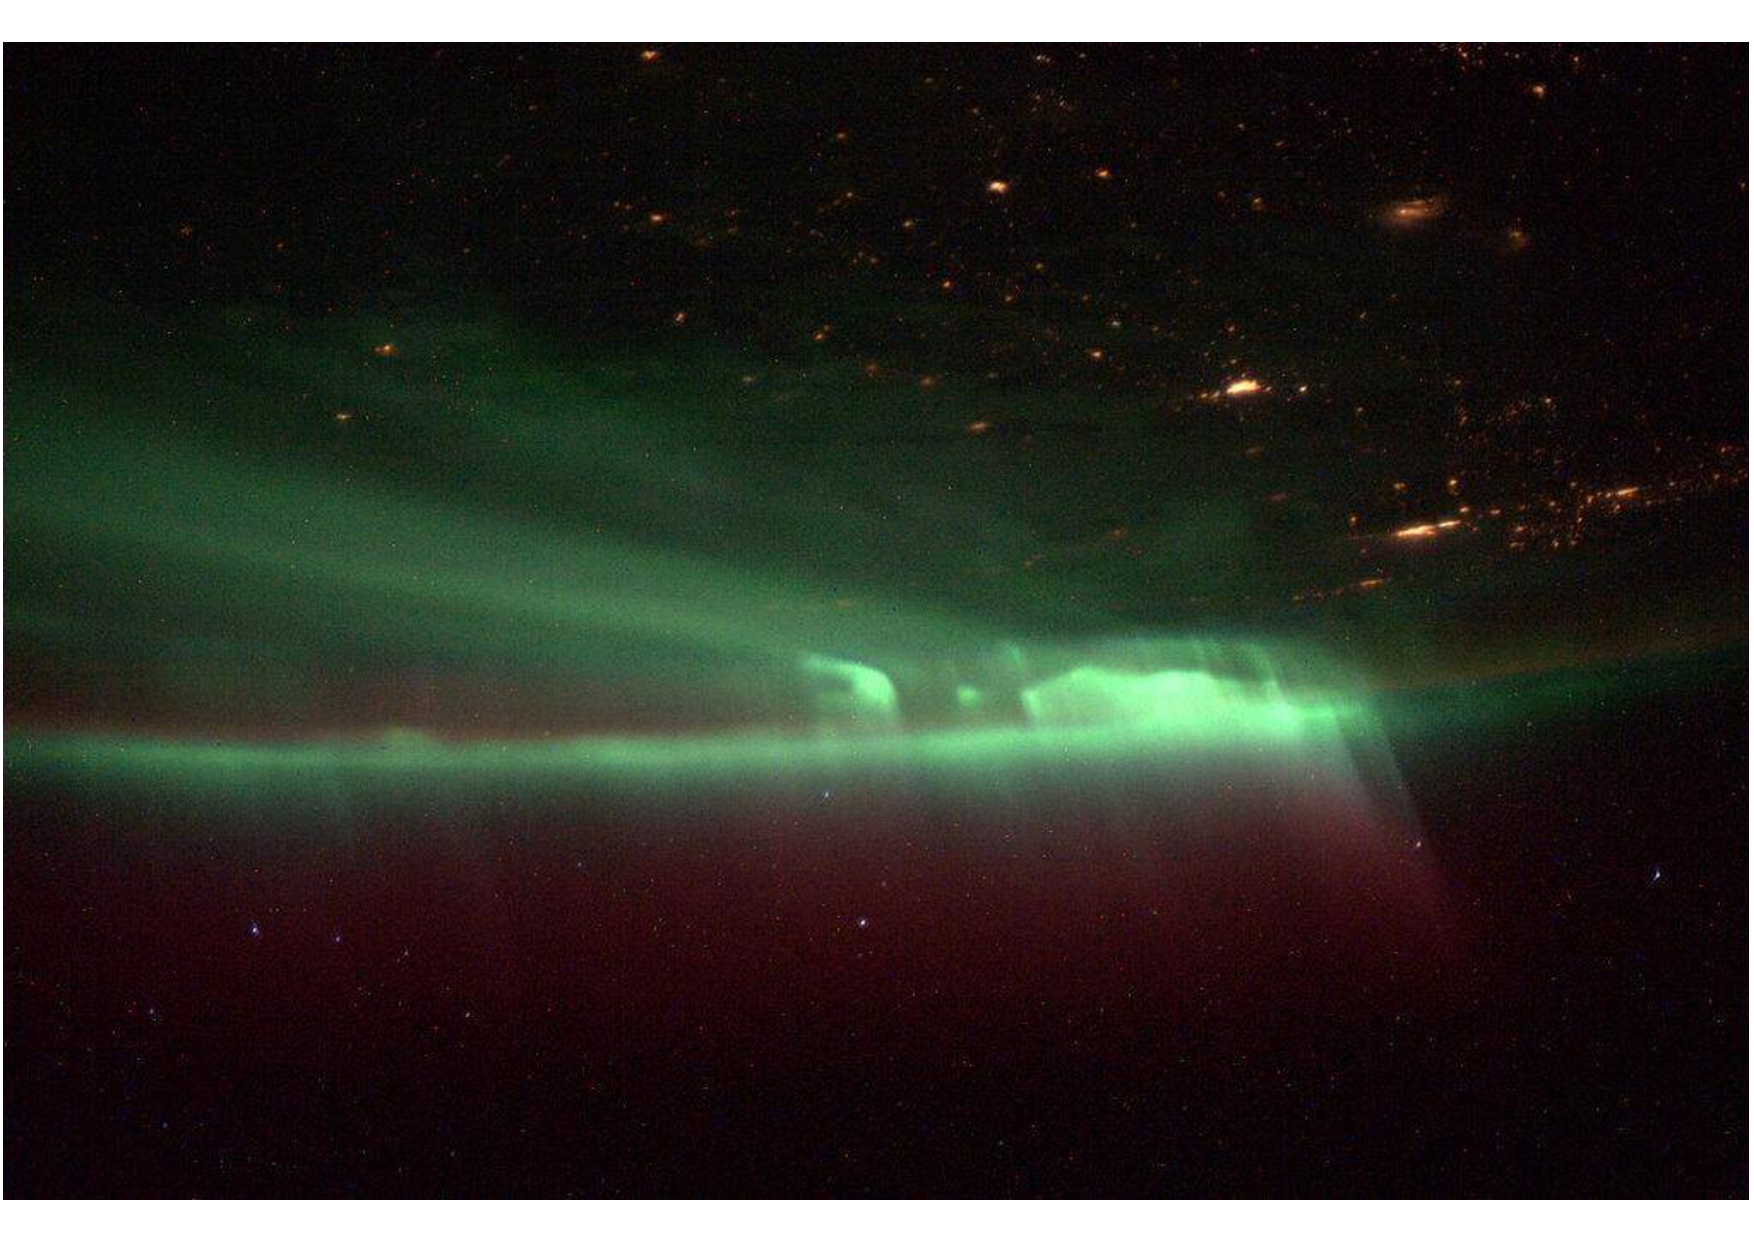
\includegraphics[scale=0.4]{Figures/1-Introduction/northern_lights_iss_20131009.pdf}
    \caption[Image of the northern lights as seen from space]{The northern lights as seen from space aboard the International Space Station. Image credit: NASA}
    \label{fig:aurora_from_space}
\end{figure}

'Magnetic activity' (commonly shortened to simply activity) is a term that is used to describe a plethora of magnetically--driven phenomena that occur on cool stars (spectral type F5 to mid-M) such as our own Sun. The study of solar magnetic activity dates back to the 17\ts{th} century, when several scientists (Johannes Fabricius, Galileo Galilei and Christoph Scheiner) independently observed black spots on the Sun's surface. They found that these black spots (now known as sunspots) would move across the face of the Sun, disappearing from one side of the Sun and reappearing on the opposite side. This led the astronomers to believe that the Sun was moving and had a rotation period. These observations have led to over 400 years of studying the Sun in detail and have given us a vast amount of information about how the Sun works. With the advancement of technology, we can now study the stars in our own Milky Way galaxy and try to establish how the Sun fits into the stellar population as a whole.

One may wonder how magnetic activity evolves in time: For example, what was the magnetic activity of the Sun like when life was just starting to evolve, or what will it be like in the future? We could also ask what the magnetic activity is like on stars of varying stellar masses; this is particularly important when considering the potential habitability of an exoplanet (that is, a planet that orbits another star other than our own Sun). It is these questions that are considered in the work presented in this thesis, by considering the age--activity--rotation relationship. While the concept of the age--activity--rotation relationship is not new science, there are limitations to previous studies, and regimes where the relationship can be improved upon. The difficulty with studying the evolution of stellar properties with time is that the ages of the stars must be known, and this is not a trivial value to calculate. While many studies use clusters as a calibration data set, these tend to be younger than a gigayear, and there are very few older than this age. There are a handful of clusters older than a gigayear, but these tend to be more distant, which makes calculation of magnetic activity indicators more difficult. The work presented in this thesis will attempt to extend the current knowledge of these age relationships by using ages determined from asteroseismology, which has become a valuable technique in determining the ages of field stars.

To begin, I will give an overview of several topics that are crucial in the understanding of the age--activity--rotation relationship. These topics include: stellar dynamo and magnetic braking (Section \ref{Section:intro_dynamo_and_braking_section}), the stellar atmosphere and the magnetic activity associated with each region (Section \ref{Section:intro_stellar_structure}) and finally, the ages of stars and methods to determine them (Section \ref{Section:intro_ages}).

\section{Stellar dynamo and magnetic braking}
\label{Section:intro_dynamo_and_braking_section}

\subsection{Stellar Dynamo Theory}
The first observation of solar magnetic fields was by \citet{Hale_1908}, where the Zeeman effect was observed in the spectrum of a sunspot. The Zeeman effect describes the interaction between atoms and the magnetic field \citep{Zeeman_1897}: The electronic energy levels of an atom will split when exposed to a magnetic field, causing multiple absorption/emission spectral lines; whereas only one spectral line would be present without a magnetic field. This raises the question: how does the Sun produce its magnetic field? The answer lies within the interior structure of the Sun: The Sun has a radiative core surrounded by a convective envelope. It is the interaction of these two layers, at the tachocline, that allows the magnetic field to be produced (known as the dynamo effect) and magnetic activity to be observed. This dynamo action is also seen in stars with spectral type ranging from F5 to $\approx$ M3 - M4, as these stars have a similar structure to the Sun, but with differing volumes of convective zone. Below a stellar mass of $\approx 0.35 M_{\odot}$, stars are expected to be fully convective and no longer have a radiative zone \citep{Chabrier_1997}. It is therefore theorised that a different type of dynamo operates in these stars that does not require a radiative zone (e.g. \citealt{Durney_etal_1993}). This is still an active research topic in the community. Conversely, stars with spectral types earlier than F5 do not have the substantial outer convective envelope that is required for the solar-like dynamo process \citep{Pinsonneault_etal_2001}.

The theory of the solar dynamo is described by magnetohydrodynamics (MHD): the study of the magnetic properties and behaviour of fluids that are electrically conducting, such as plasma in stars. While the full details of the solar dynamo are not yet fully understood, the most accepted theory is the $\alpha\Omega$ dynamo \citep{Choudhuri_2007}. If we consider an ordinary electromagnetic dynamo, a conducting coil rotates in a magnetic field and cuts through magnetic flux lines thus producing an electromotive force (e.m.f.) by Faraday's Law of Induction. In stars, there are rotating regions of plasma that can also induce an e.m.f., and in favourable conditions the e.m.f. can reinforce the magnetic field. Therefore, the dynamo process can build up a magnetic field starting from an initial seed field. This initial seed field comes from the gas cloud that the star formed from, since observations of such gas clouds show that they have a magnetic field associated with them. It is known that the Sun does not rotate as a solid body; but rather, the equator spins $\approx 20 \%$ faster than the poles. This is an important factor in dynamo theory, as it can also be shown that the magnetic field is frozen in the plasma and moves with it. This is Alfve\'n's theorem of flux-freezing \citep{Alfven_1942}. It is because of differential rotation and flux freezing that the poloidal magnetic field is then stretched out in the toroidal direction. This is shown in the middle panel of Figure \ref{fig:dynamo} and is known as the $\Omega$ effect. This $\Omega$ effect takes place in the region where differential rotation is at its greatest; helioseismology has found that this region is known as the tachocline and is located at the bottom of the convection zone. Therefore, it is expected that the strongest toroidal field will be at the tachocline.

\begin{figure}
    \centering
    \captionsetup{width=.9\linewidth}
    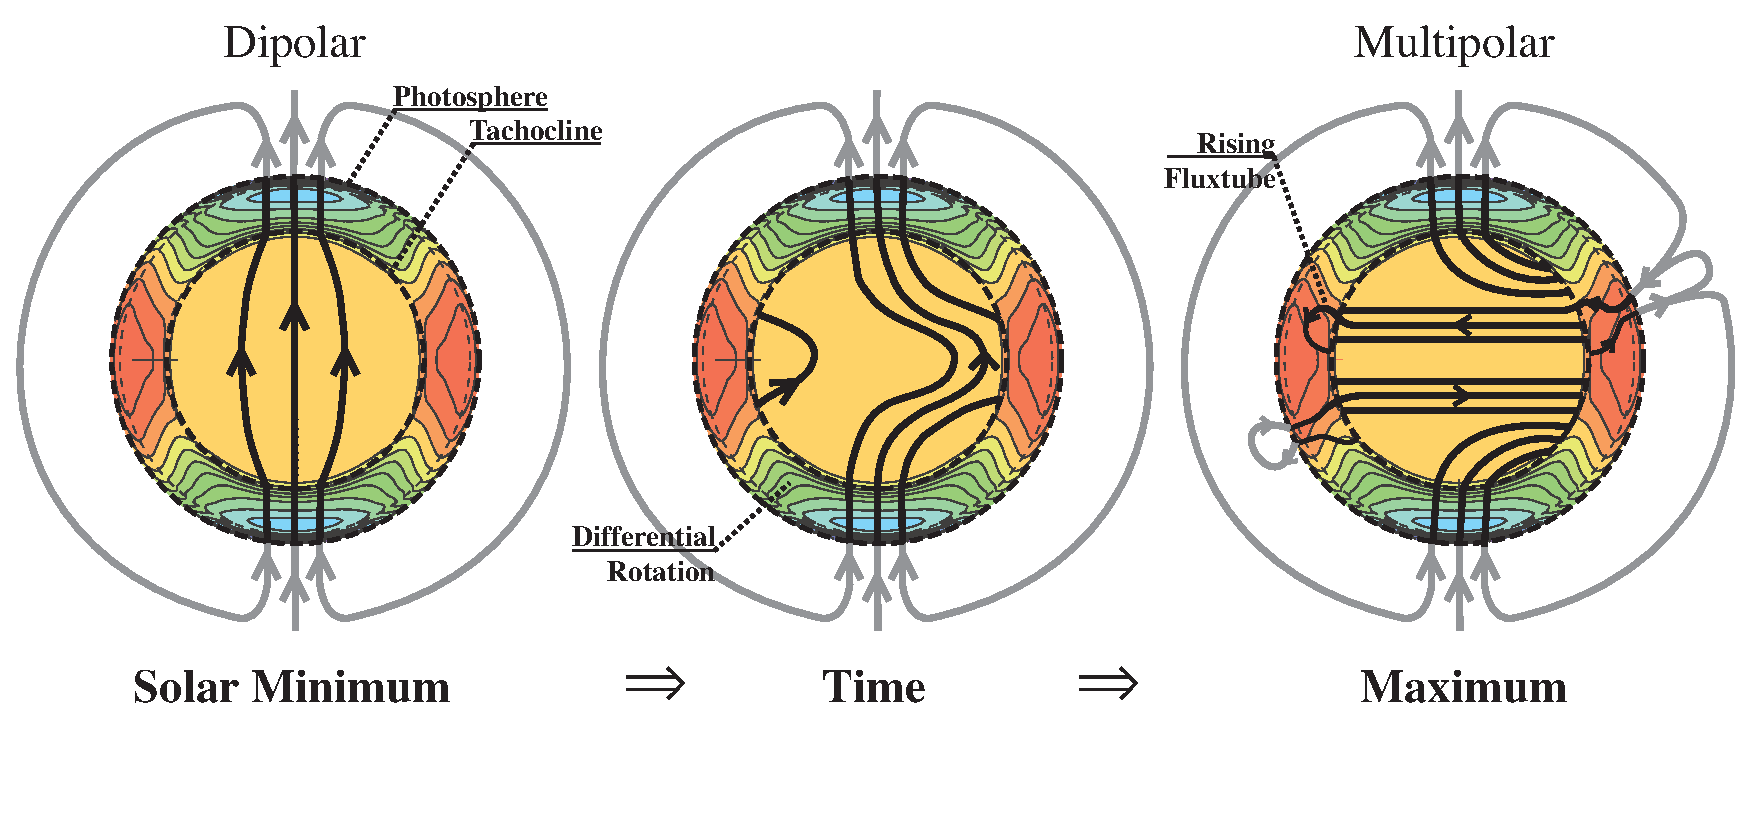
\includegraphics[width=.9\linewidth]{Figures/1-Introduction/dynamo_schem.eps}
    \caption[Schematic of the solar dynamo]{A schematic of the solar dynamo, showing the interior and magnetic field lines of the Sun over time, from solar minimum to solar maximum. The colours show the rate of rotation within the Sun, where red indicates a faster rate of rotation and blue indicates a slower rate of rotation. Over time, the differential rotation in the convection zone causes the poloidal field to be stretched in the toroidal direction. As the magnetic fields become sheared and twisted they become "flux-ropes" and magnetic buoyancy causes them to rise to the solar surface. At solar maximum these flux-ropes appear at the solar surface, causing the solar magnetic field to become multipolar. Image credit: \citet{higgins_2012}}
    \label{fig:dynamo}
\end{figure}

Another important aspect of the solar dynamo is the interaction of the magnetic field with the convection in the plasma (known as magnetoconvection). Numerical simulations by \citet{Weiss_1981} studied the nonlinear evolution of convection in the presence of a magnetic field: they found that two different regions formed. In the first region, magnetic field is excluded and vigorous convection takes place. In the second region, the magnetic field gets concentrated and the tension of the magnetic field lines suppresses convection. In the latter regions, flux tubes form which are concentrated bundles of magnetic field lines. In regions of strong differential rotation (such as the tachocline), these flux tubes will align with the toroidal field and if they have magnetic buoyancy, they can rise to the surface of the star. Flux tubes that pierce the solar surface can form bipolar spots: these are spots close together with opposite polarities. From these sunspots, some of the toroidal magnetic field is converted back into poloidal field, but the exact mechanism is still an open question.

The most likely mechanism is known as the Babcock-Leighton mechanism \citep{Babcock_1961,Leighton_1969}. It is known that bipolar spots have a tilt associated with them that increases with increasing latitude (known as Joy's Law), therefore one spot is closer to the equator than the other. Each spot diffuses its polarity at different latitudes, which then forms a poloidal field at the solar surface. These field lines then migrate towards the pole through the meridional circulation, which is the constant flow of plasma near the Sun's surface from the equator to the pole. The field lines can then flow to the tachocline from the poles by the counterpart to the meridional circulation which must exist as we do not not observe an excess of material at the pole. Thus completes the solar dynamo cycle, and the process can repeat.

\subsection{Angular momentum evolution of stars}

All stars are formed with an initial amount of angular momentum that comes from the formation process, but the angular momentum is not constant over the lifetime of the star. In this section I will give a brief overview of how the angular momentum changes throughout a solar--type star's lifetime. Figure \ref{fig:gallet_&_bouvier_2013_fig} shows the angular velocity as a function of age for solar--type stars in star-forming regions and young open clusters. The large distribution of angular velocities in these stars is due to the initial angular momentum that each star was born with. However, once solar-type stars reach $\approx 1$ Gyr, they converge to a similar angular velocity.

\begin{figure}[h]
    \centering
    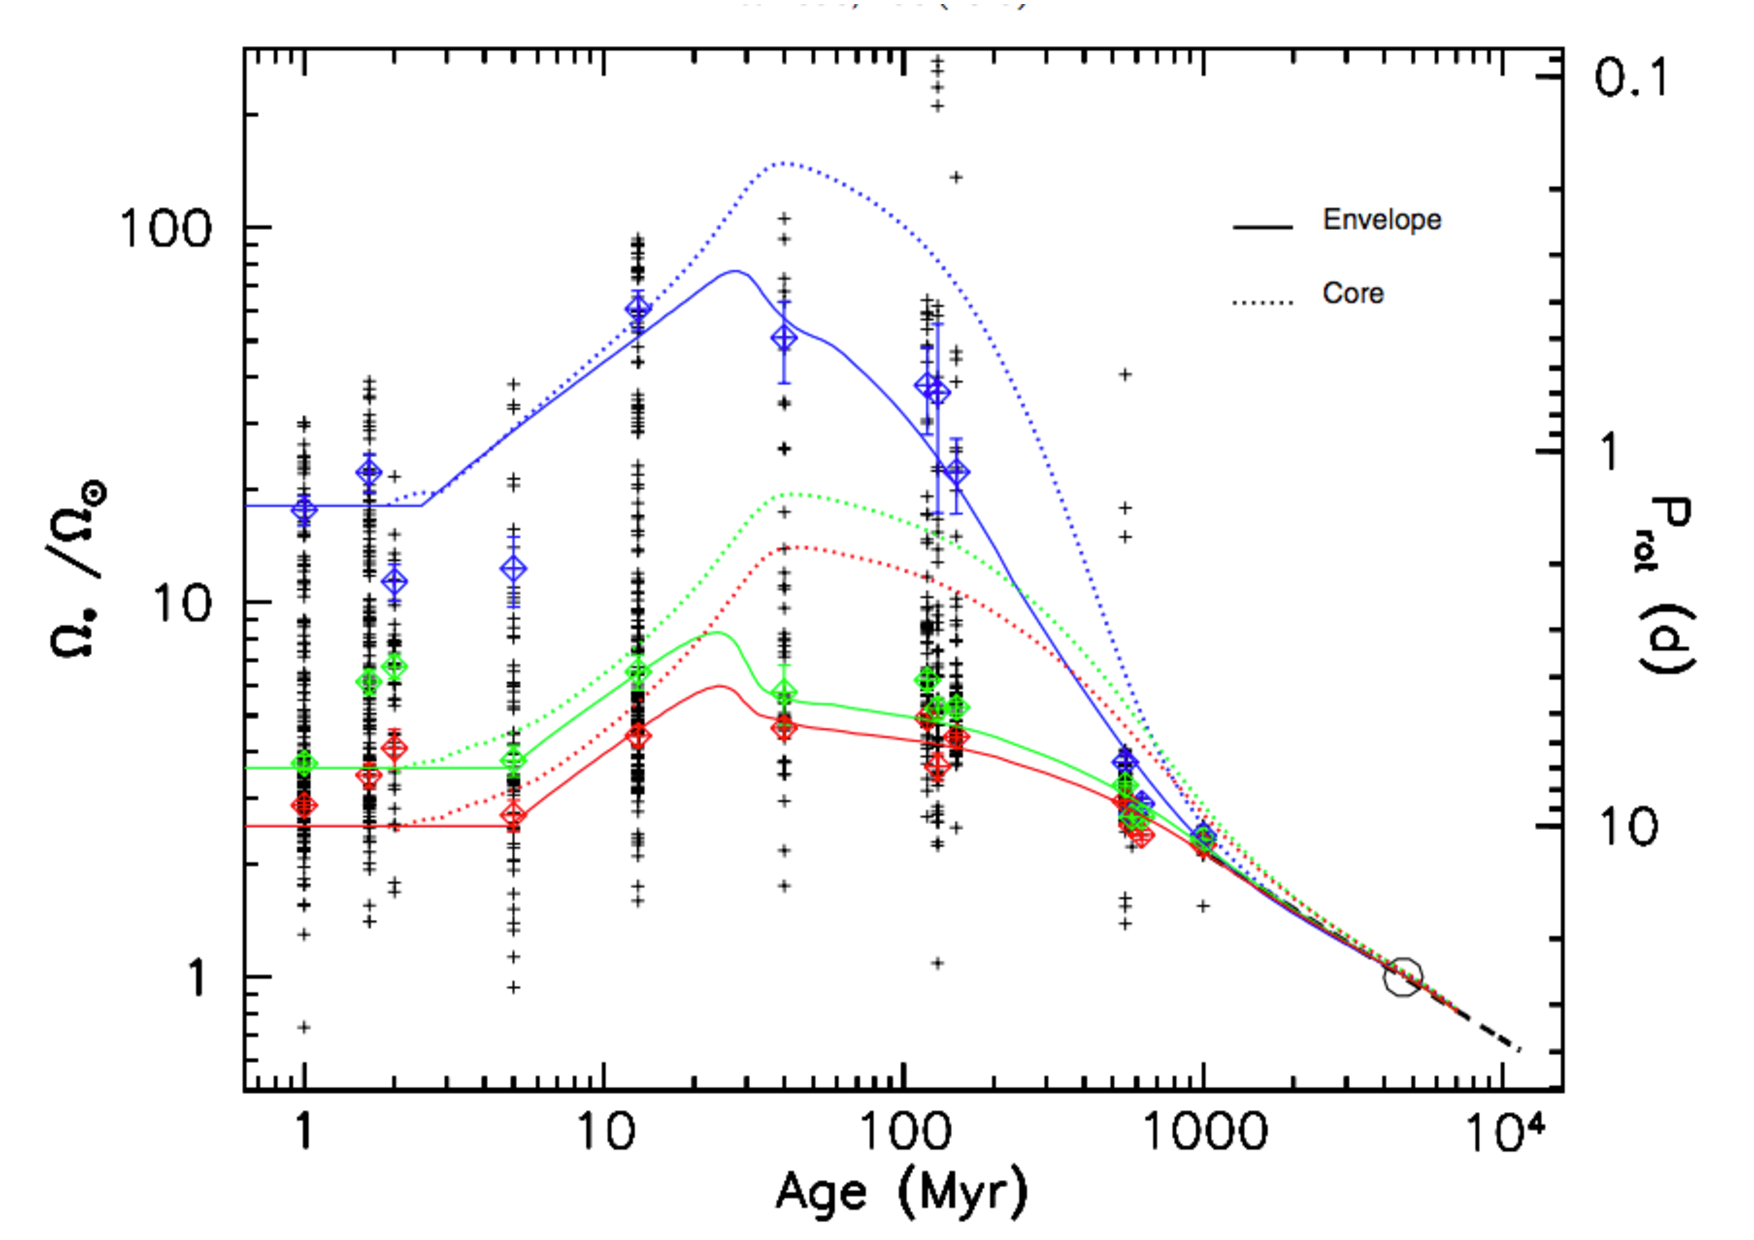
\includegraphics[scale=0.4]{Figures/1-Introduction/gallet&_bouvier_figure_2013.pdf}
    \caption[Angular velocity distribution as a function of age]{Figure from \citet{Gallet_Bouvier_2013} that shows the angular velocity distribution of solar--type stars in star--forming regions and young open clusters as a function of age. Also plotted are the angular velocity of the radiative core (dashed lines) and convective envelope (solid lines) as a function of time for fast (blue), median (green) and slow (red) rotator models. The open circle represents the angular velocity of the Sun. The black dashed line represents the Skumanich law.}
    \label{fig:gallet_&_bouvier_2013_fig}
\end{figure}

During the pre-main-sequence (henceforth PMS), despite the fact that these stars are still contracting from their formation, they are prevented from spinning up due to interactions with their accretion disk \citep{Edwards_etal_1993,Rebull_etal_2004}. This period lasts for a few million years until the accretion disk disappears. The star then continues to spin up due to contraction from its formation until it reaches the zero age main sequence (henceforth ZAMS). Once the star is on the main sequence (henceforth MS) then angular momentum is lost from its magnetised stellar wind in a process called magnetic braking.

Figure \ref{fig:gallet_&_bouvier_2013_fig} shows the angular velocity distribution of solar--type stars in star--forming regions and young open clusters as a function of age from \citet{Gallet_Bouvier_2013}. \citet{Gallet_Bouvier_2013} presented rotational evolution models that were able to reproduce the distribution of stellar rotation periods and how they converged on the MS. An important aspect of the models shown in Figure \ref{fig:gallet_&_bouvier_2013_fig} is the distribution of angular momentum within the interior of the stars, as this is crucial to the understanding of why all the stars converge to a similar rotation period on the MS. If a star has strong core-envelope coupling, then the whole star reacts to angular momentum that is lost at the stellar surface, resulting in a long-term steady decline of the surface velocity. However, in decoupled models, the radiative core retains most of the initial angular momentum, while the convective envelope may lose angular momentum. Then at later times in the decoupled model, the angular momentum stored in the core of these stars can be redistributed to the convective envelope, thus delaying the spin down phase. This is the key difference between the fast and median/slow rotator models. In fast rotator models, the core-envelope coupling has a relatively short timescale of 12 Myr. In contrast, the slow and median rotator models have a core-envelope coupling timescale of 28-30 Myr which allows the convective envelope to be efficiently braked before the ZAMS. The core-envelope coupling also explains the difference in shape of the rotational tracks: slow and median rotators have a much flatter rotational evolution on the the early MS, as angular momentum is being slowly transferred back into the envelope from the core.

The work in this thesis focuses on the angular momentum lost while solar and late-type stars are on the the main sequence. \citet{Schatzman_1962} first proposed that stars could lose angular momentum through their magnetised stellar wind. Material that is lost from the stellar surface (e.g. through solar wind or flares) is forced to co-rotate with the stellar surface by the magnetic field up until a critical distance, known as the Alfve\'n radius. The Alfve\'n radius is defined as the point where the magnetic energy density is equal to the kinetic energy density: beyond this point, the material is said to be lost from the star and carries away some angular momentum. The seminal analysis of this process was performed by \citet{Weber_&_Davis_1967}, who modelled the solar wind angular momentum loss in the idealised case of a simple monopole magnetic field. A key result of this analysis is shown in Equation \ref{Eq:WD67_mag_braking}. This shows that the rate at which the star loses angular momentum depends on several factors: the angular velocity at the stellar surface ($\Omega_{*}$), the mass loss due to the stellar wind ($\dot{M}_{wind}$) and the Alfve\'n radius ($r_{A}$). Note that the Alfve\'n radius depends on the stellar magnetic field.

\begin{equation}
    \frac{dJ}{dt} = \frac{2}{3}\Omega_{*}\dot{M}_{wind}r_{A}^{2}
    \label{Eq:WD67_mag_braking}
\end{equation}

Since this seminal analysis on the angular momentum loss, great progress has been made with more sophisticated, physics-based models that incorporate mass \citep{Matt_etal_2015}, magnetic field geometries \citep{Finley_etal_2017,Garraffo_etal_2018} and coronal temperature \citep{Pantolmos_etal_2017}, to name a few. However, the generation of the magnetic field is also linked to the rotation of the star through the stellar dynamo. Therefore, as the star loses angular momentum we would expect both the rotation period and magnetic activity of the star to decrease with time. This has led to many studies on the evolution of these parameters with age, which will be discussed in Chapter \ref{Chapter2}. Consequently, the change in the magnetic field of the star will also affect the efficiency of the magnetic braking, thus creating a dependency between  stellar age, activity and rotation.

\section{Stellar atmosphere and magnetic activity}
\label{Section:intro_stellar_structure}

All stars form from clouds of gas and dust that collapse under their own gravitational force. The centre of the cloud becomes hotter and more dense until the correct conditions are met for nuclear fusion to begin and a star is born. While all stars are essentially astronomical bodies that burn hydrogen into helium at their cores (at some stage in their life), the mass of the star has a strong influence over the structure of the star and consequently its evolution. In this work, I concentrate my studies on stars with spectral type ranging from F5 to $\approx$ M3 ($1.33 M_{\odot} - 0.35 M_{\odot}$) because the structure of these stars allows for the manifestation of magnetic activity. These solar- and late-type stars have a radiative core surrounded by a convective envelope, and it is the interaction of these two layers that allows the magnetic field to be produced (see Section \ref{Section:intro_dynamo_and_braking_section}) and magnetic activity to be observed. Therefore, any further discussion about stellar structure will be in relation to this range of the stellar population. Magnetic activity is observed from the atmosphere of a star, where we define the atmosphere as the region where photons can escape directly into space. In this section, I will outline the different layers of the stellar atmosphere and the types of magnetic activity seen in each region. At first, I will focus on solar observations, as we can resolve the surface of the Sun and study any features in great detail. I will then explain how we study these features on other stars and in particular, how we can measure the strength of the stellar magnetic activity using these features.

\subsection{Photosphere}
\label{Chp1_photosphere}

The lowest part of the solar atmosphere is known as the photosphere. This region is only several hundred kilometres thick, yet it is the region that emits most of the solar radiation. This is the part of the Sun that we can see with our naked eye, and it is commonly referred to as the "surface" of the Sun. The surface of the Sun is defined at the optical depth of $\tau = 1$. Optical depth is a measure of the transparency of a medium and is defined by Equation \ref{Eq:optical_depth_eq} where $I$ is the amount of outgoing radiation, $I_{0}$ is the amount of incident radiation and $\tau$ is the optical depth. Therefore, at an optical depth of one, the radiation has fallen by a factor $e$.

\begin{equation}
    I = I_{0}e^{-\tau}
    \label{Eq:optical_depth_eq}
\end{equation}

The main diagnostic for magnetic activity in the photosphere is sunspots: dark regions that appear on the surface of the Sun. They have been observed for many centuries; naked eye observations date back to 165 BC \citep{Wittmann_1987}, while telescope observations started in 1611 with the rediscovery of sunspots by Galilei, Scheiner and others. Sunspots are characterised by three regions: a dark core, the umbra, and the penumbra. An example of a complex sunspot is shown in Figure \ref{fig:sunspot_example}. Sunspots occur in active regions of the Sun where the magnetic field is more intense. This inhibits convection and reduces the effective temperature of that region compared to the surrounding photosphere (typically 2000 K cooler), thus appearing darker. The size and lifespan of sunspots are tied to the strength of the magnetic field, therefore longer lasting spots typically have stronger associated magnetic fields. The typical lifetime of a spot on the Sun is on the order of hours to weeks, and most last a stellar rotation \citep{Bradshaw_Hartigan_2014}.

\begin{figure}
    \centering
    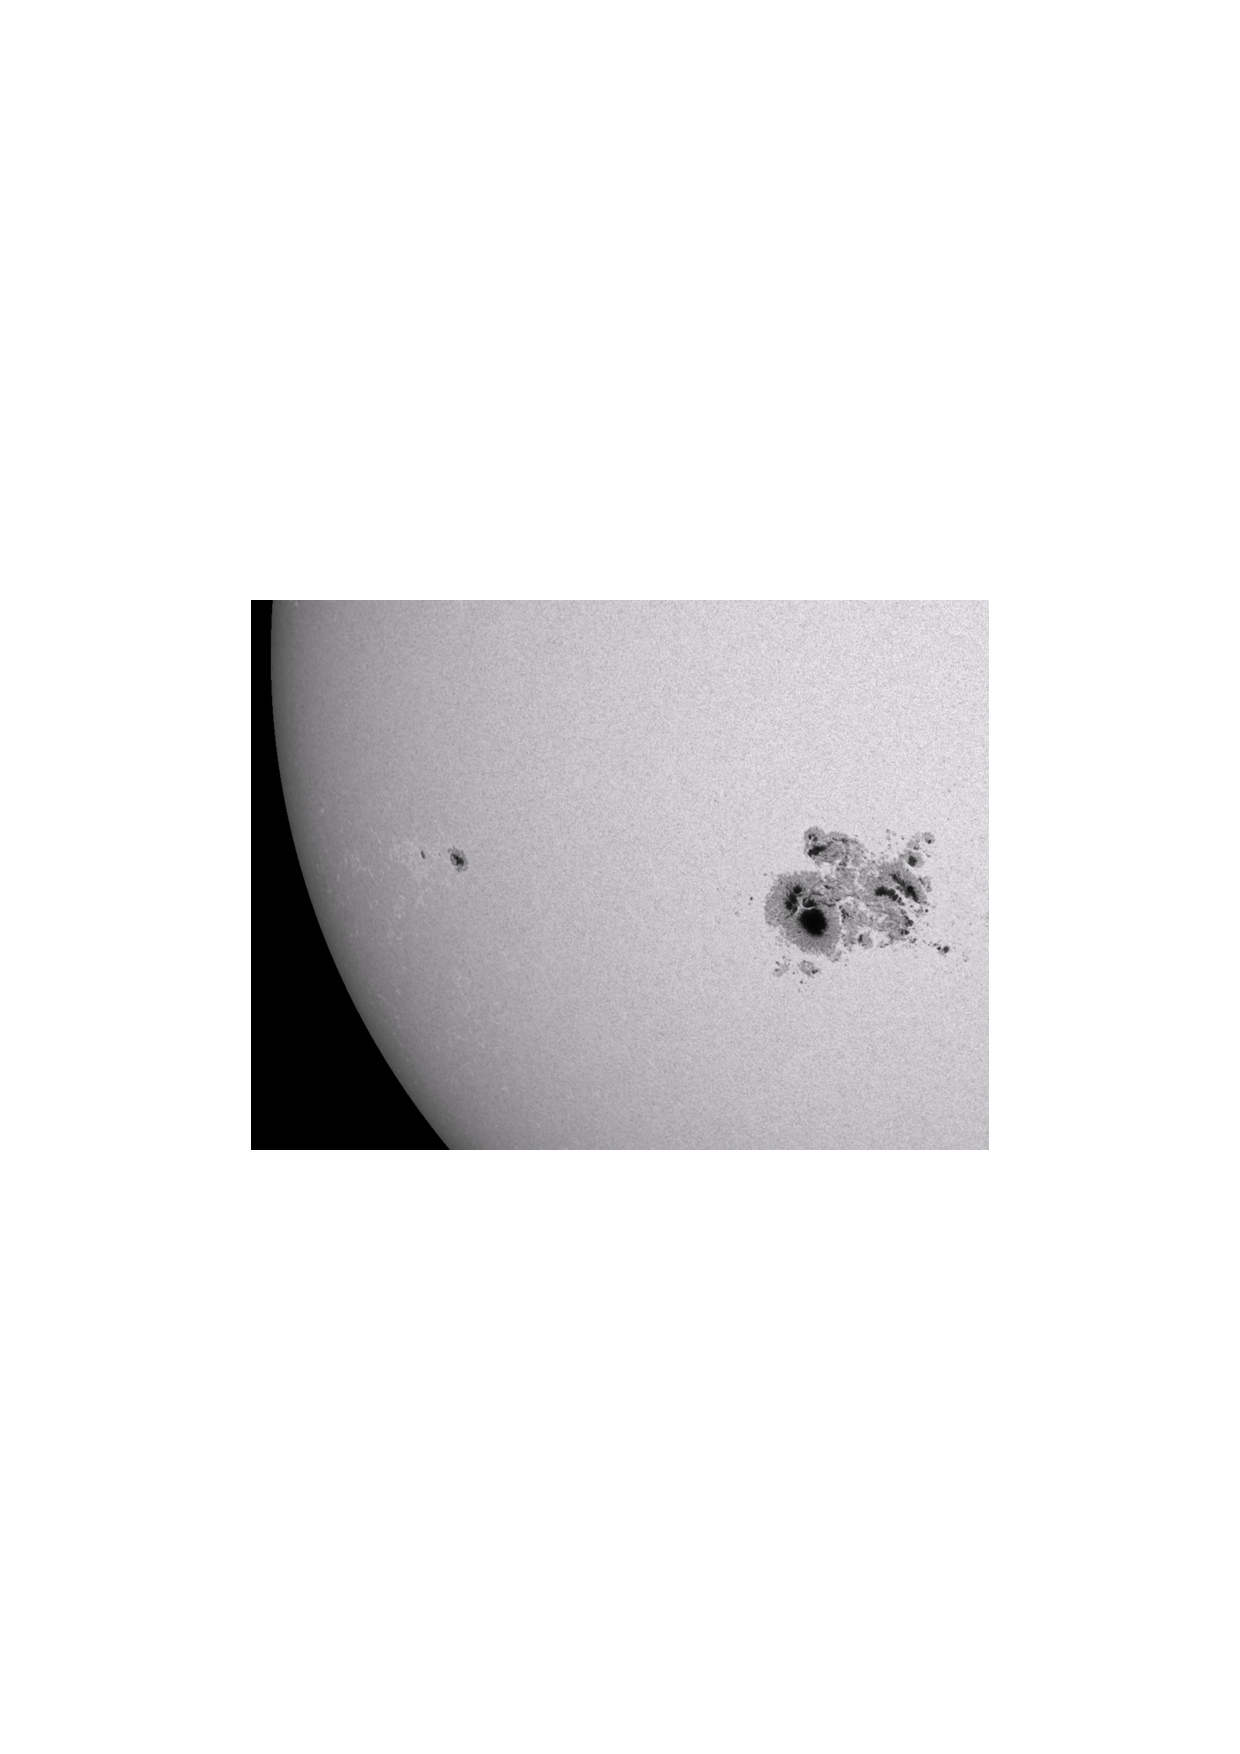
\includegraphics[scale=0.7]{Figures/1-Introduction/HMI_spot_Oct}
    \caption[Example of complex sunspot as seen by NASA's SDO]{Large, complex sunspot seen from NASA's Solar Dynamics Observatory from October 2014. Image Credit: NASA/SDO and the AIA, EVE, and HMI science teams.}
    \label{fig:sunspot_example}
\end{figure}

The observations of sunspots have lead to a better understanding of some of the internal processes at work within the solar interior. As early as the 1800's scientists were noticing patterns in the way sunspots evolved in time. \citet{Schwabe_1844} found that the occurrence of spot groups and spotless days repeated with a period of approximately 10 years. The modern day value of this period is 11 years and is known as the Schwabe solar cycle (or, more commonly, the solar cycle). \citet{Carrington_1858} noticed that sunspots seemed to appear at different latitudes over time and this was later visualised by \citet{Maunder_1904} in the now infamous "butterfly diagram". An example of such a diagram is shown in Figure \ref{fig:butterfly_diagram}, where we see that at the start of each solar cycle sunspots tend to form at mid-latitudes and then migrate towards the equator over time.

\begin{figure}
    \centering
    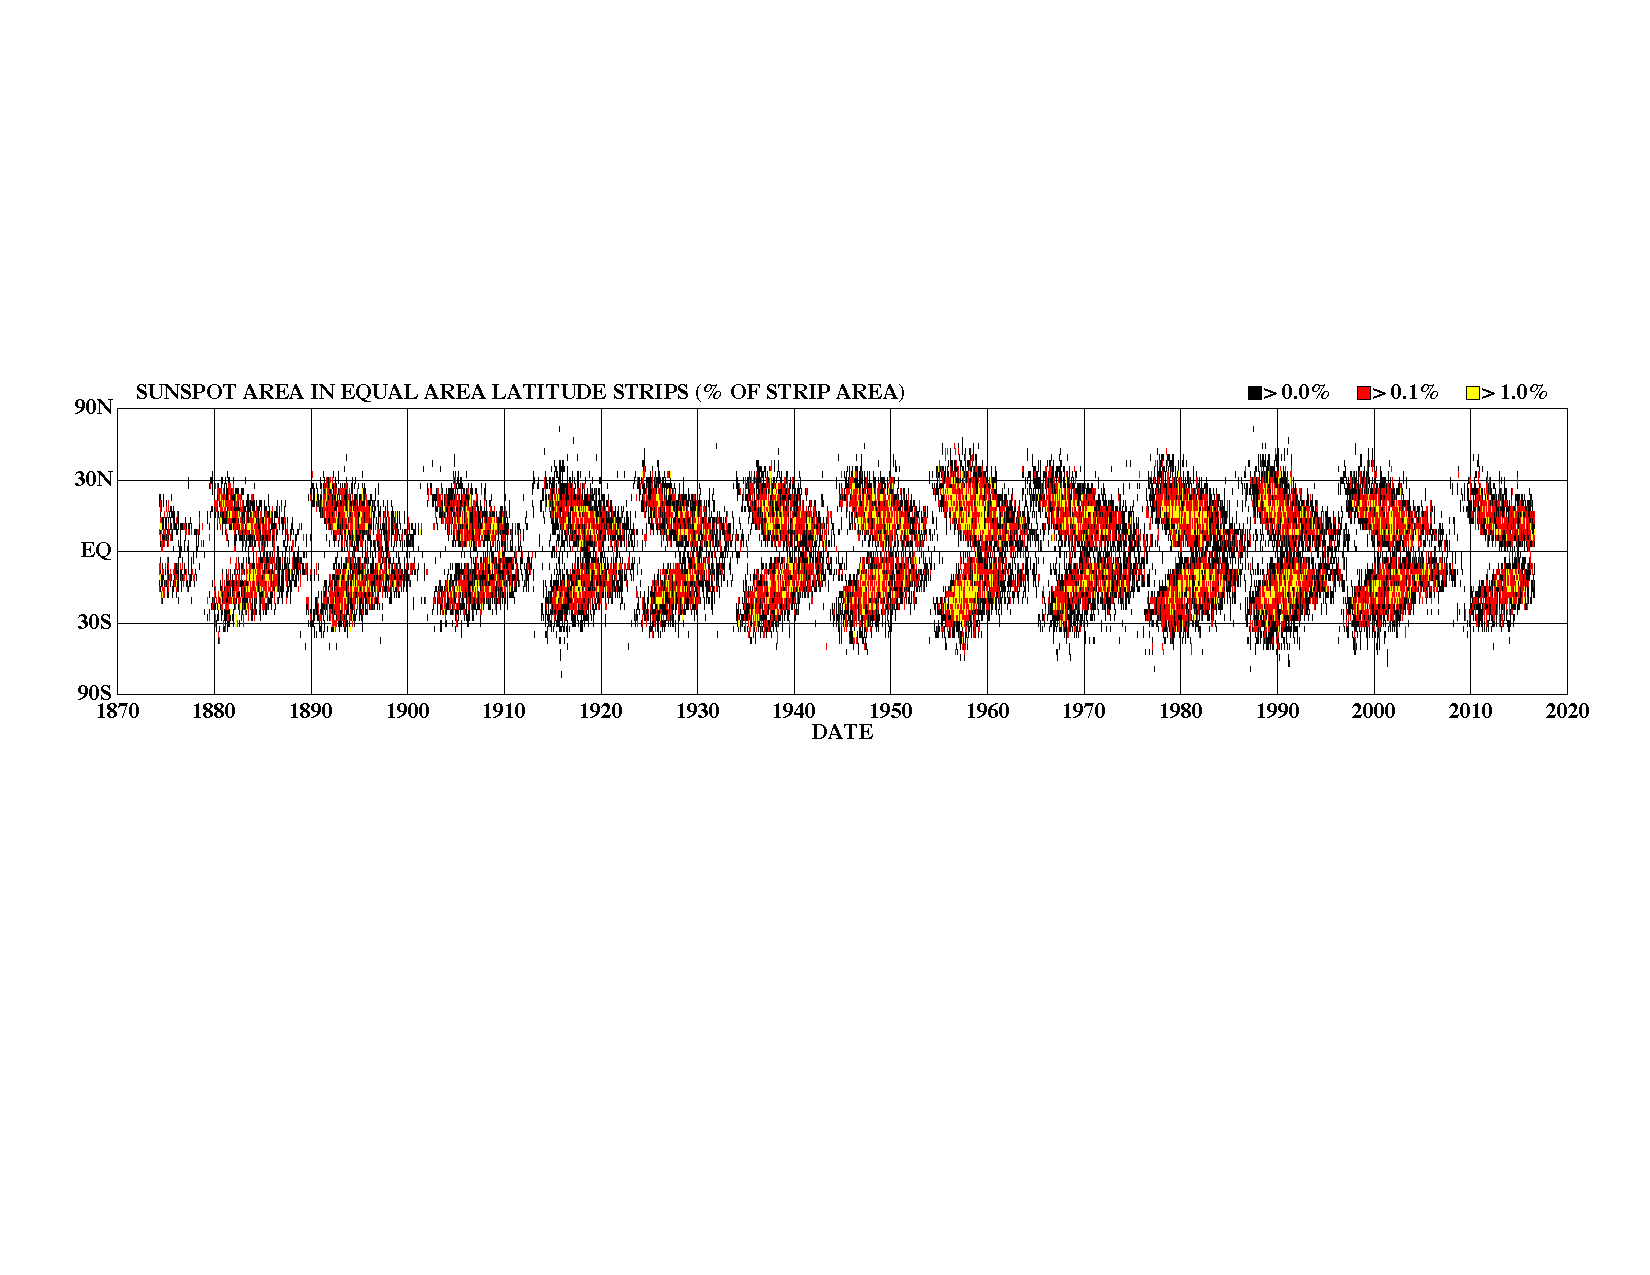
\includegraphics[scale=0.5]{Figures/1-Introduction/butterfly_diagram_crop.pdf}
    \caption[Butterfly diagram showing the latitudes of sunspots over a solar cycle]{An example of a butterfly diagram that shows the latitude of the sunspot as a function of time. At the start of each cycle, spots tend to form at mid-latitudes migrate towards the equator. Image credit:\\ \url{https://solarscience.msfc.nasa.gov/SunspotCycle.shtml}}
    \label{fig:butterfly_diagram}
\end{figure}

One paper in particular noted several patterns that would become useful constraints for solar dynamo theories. \citet{Hale_etal_1919} devised a method of determining the angle between the magnetic field vector on the Sun and the line-of-sight, which allowed the polarity of sunspots to be investigated. Firstly, they found that spots would frequently appear in pairs with the preceding member forming first. Secondly, the axis of a binary spot group formed a small angle with the equator, with the leading spot closest to the equator. This angle also tended to increase for higher latitudes, and is now known as Joy's Law. Thirdly, the two members of a binary spot group would be of opposite polarity. The polarity of the leading/following spot would be the same for bipolar spots in the same hemisphere, and would be the opposite for bipolar spots in the other hemisphere; this is known as Hale's Law. Lastly, after the solar cycle minimum, the polarity for the leading/following members in bipolar spots reverses in each hemisphere. This is known as the Hale magnetic cycle, and comprises of two solar cycles.

\begin{figure}[t]
    \centering
    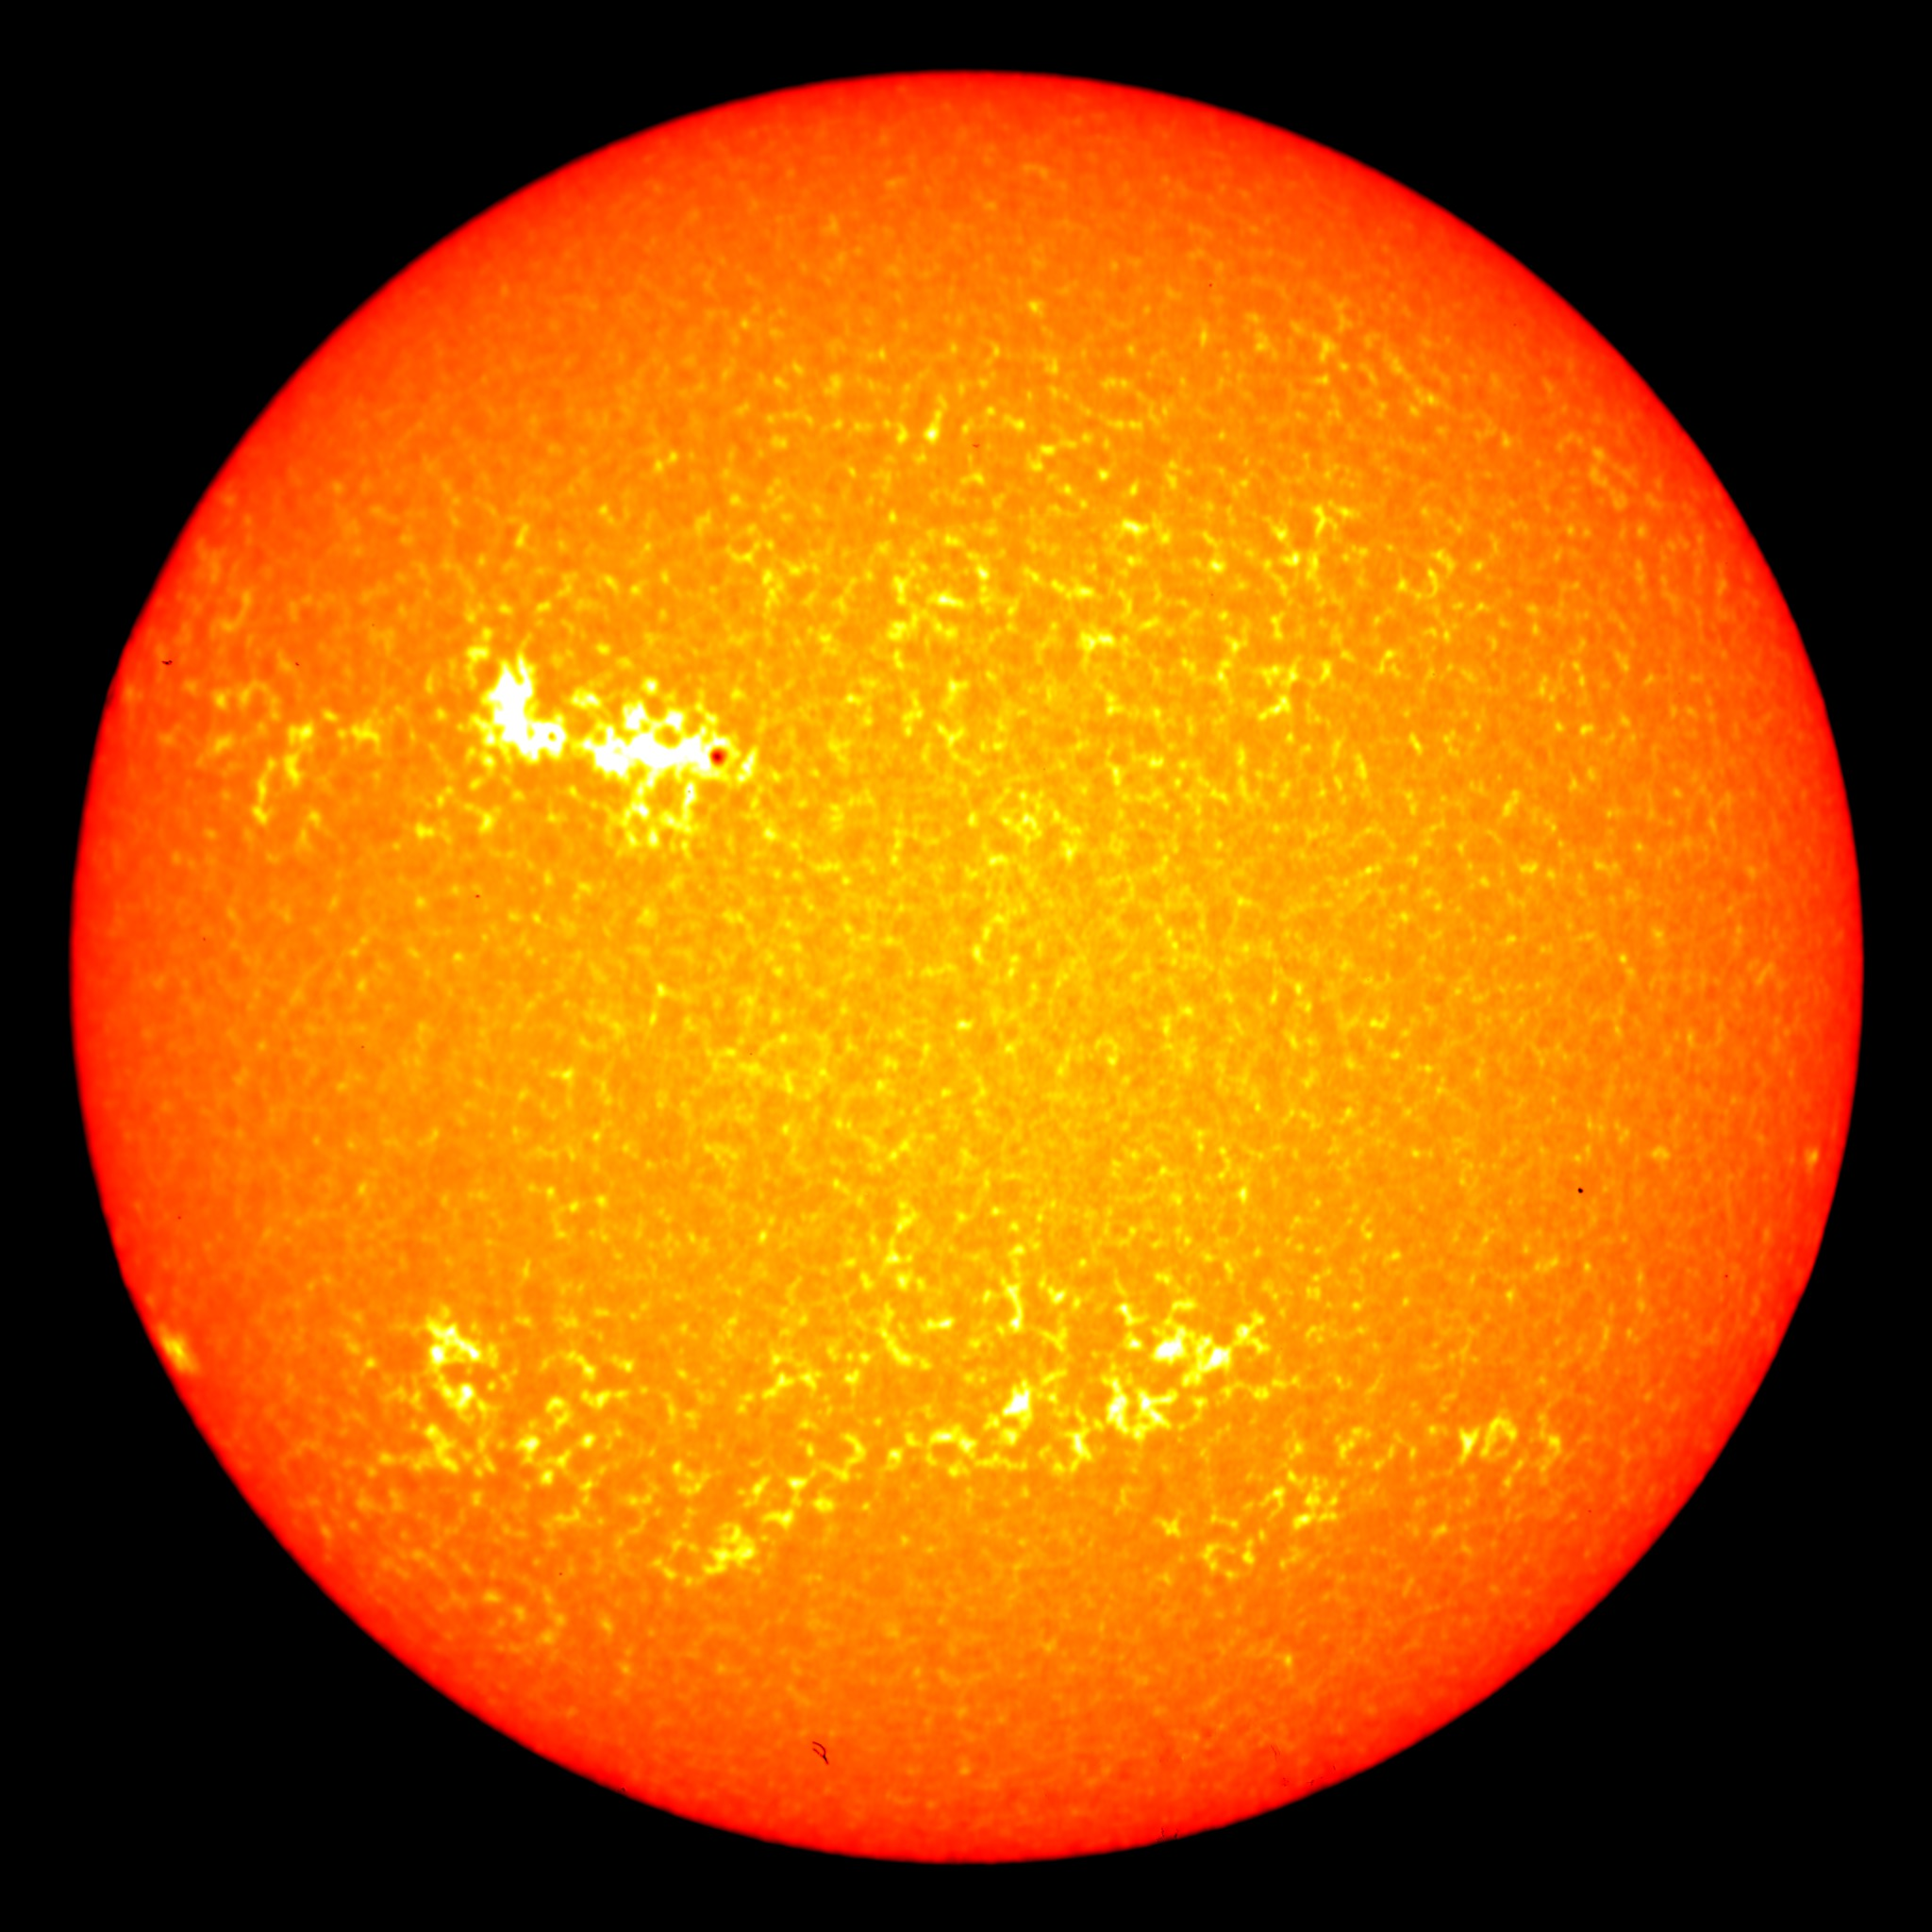
\includegraphics[scale=0.15]{Figures/1-Introduction/faculae_example.jpg}
    \caption[Example of faculae during a period of low activity on the Sun]{View of the Sun during a period of low activity in October 1998. The colour table has been altered to enhance the appearance of faculae which are seen as the bright white regions. Faculae appear near a small sunspot and in other regions with no sunspots. Image credit: NASA/Goddard Space Flight Center Scientific Visualization Studio. Source data courtesy of HAO \& NSO PSPT project team.}
    \label{fig:faculae_example}
\end{figure}

Another magnetic feature present in the photosphere are bright, small-scale regions known as faculae \citep{Hale_1922}. While faculae and similar features called plage are both spatially--associated, and the two terms are often used synonymously, they form in different stellar regions: faculae form in the photosphere while plage form in the chromosphere. Faculae are regions of increased magnetic field which, unlike sunspots, are not strong enough to inhibit convection. Instead, the increased magnetic field alters the opacity at the surface, allowing for a deeper view into the photosphere where it is hotter and therefore brighter. Faculae have a lower contrast with the surrounding photosphere, therefore they are best viewed near the limb of the Sun. Figure \ref{fig:faculae_example} shows an image of the Sun during a period of low activity in October 1998 (note that the colour table has been altered in order to enhance the appearance of faculae). The faculae are shown as bright white regions and we see that they appear near a small sunspot in the northern hemisphere but also appear in the southern hemisphere where no sunspots are present. Since there is a lower magnetic field threshold for faculae, they tend to be longer--lived and more abundant across the stellar disc than sunspots. This means that during solar maximum, there are large number of faculae resulting in an increase in the solar irradiance \citep{Walton_etal_2003}, despite the increased prevalence of sunspots.

It stands to reason that since the Sun exhibits dark spots, other stars with a similar structure would also exhibit spots. Photometric observations of stars with starspots date back to \citet{Kron_1947}, when eclipsing binaries were studied and significant variation in the light curve was detected outside of the eclipse. It was theorised that this was due to light and dark patches on the surface of the star. Later \citet{Hall_1972} demonstrated that a model that included a region of starspot activity could reproduce the peculiarities in the data.

Since starspots move across the stellar surface at the same rate as the surface, the modulation in the light curve due to starspots can be used to determine the rotation period of the star. These rotation periods are much more reliable than measurements made from spectroscopic data, as they are not dependent on the inclination of the star. To determine the rotation period, observations are needed over the timescale of the rotation period and ideally for several rotation periods; this means that observations tend to be biased towards faster rotators that have shorter rotation periods. In addition to this, observations are also biased towards younger stars, as they are much more active than older stars and have more detectable modulations in photometric observations. However, progress is being made towards determining rotation periods for older and more slowly rotating stars (e.g. \citealt{Barnes_etal_2016,Douglas_etal_2016,Lanzafame_etal_2018}). Space telescopes such as \textit{Kepler}/\textit{K2} have been instrumental in this progress as they continuously monitor stars for long periods of time and produce light curves spanning long periods of time that are ideal for determining rotation periods.

\begin{figure}
    \centering
    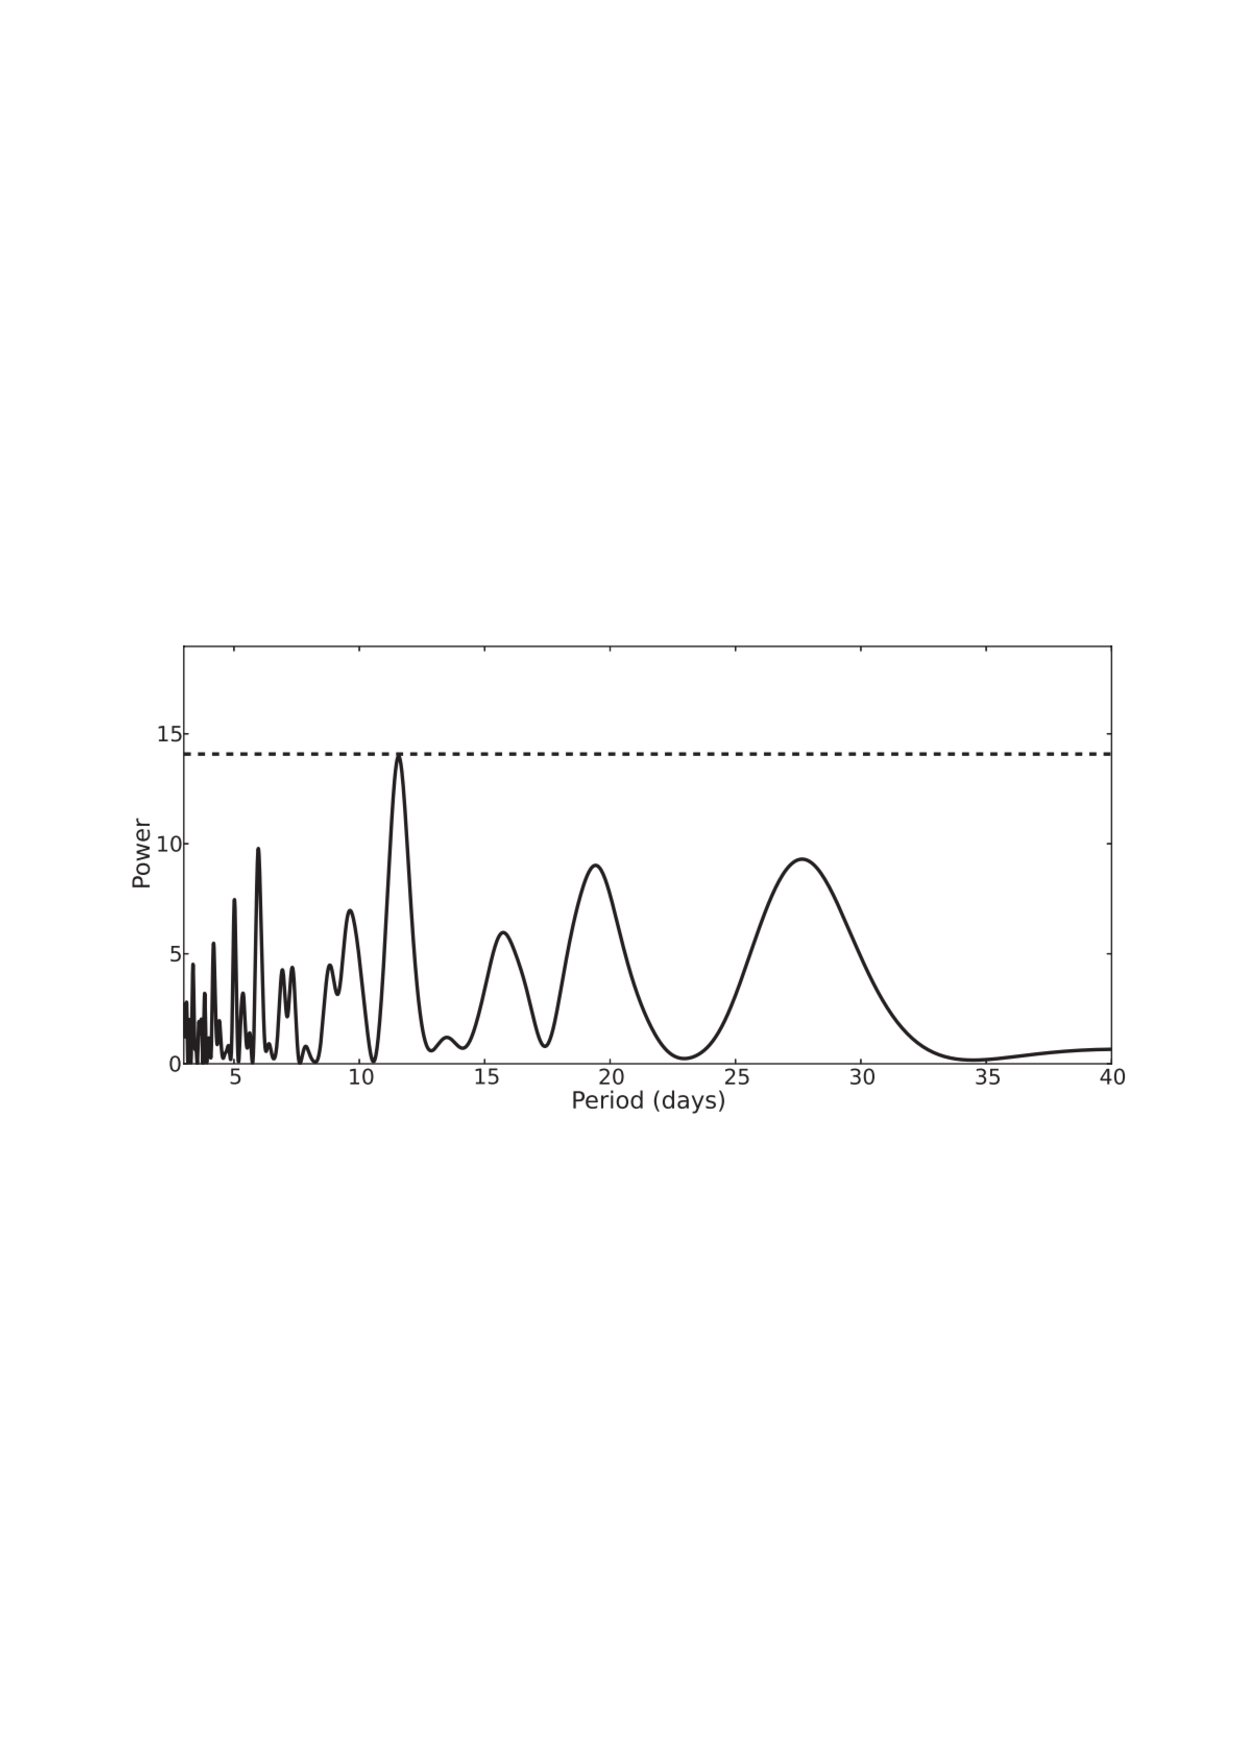
\includegraphics[width=0.9\textwidth]{Figures/1-Introduction/brothwell_2014_LSP.pdf}
    \caption[Lomb Scargle periodogram example]{Example of a Lomb--Scargle periodogram for the WASP 32 system. The dashed line represents the false alarm probability of 0.1 per cent. The peak period corresponds to a rotation period of 11.6 days. Image credit: \citet{Brothwell_etal_2014}}
    \label{fig:LS_periodogram_example}
\end{figure}

A common method of determining rotation periods from starspot modulation is to use a Lomb--Scargle periodogram \citep{Lomb_1976,Scargle_1982}. This method takes a Fourier transform of the light curve to search for periodicities; since starspot modulations are sinusoidal in nature this will appear as a delta function in the Fourier transformation. Generally a distribution of delta peaks will appear in the power spectrum of the data similar to the example shown in Figure \ref{fig:LS_periodogram_example}. When considering the rotation period, it is appropriate to choose the period with the largest Lomb Scargle power \citep{Nielsen_Karoff_2012}.

\begin{figure}
    \centering
    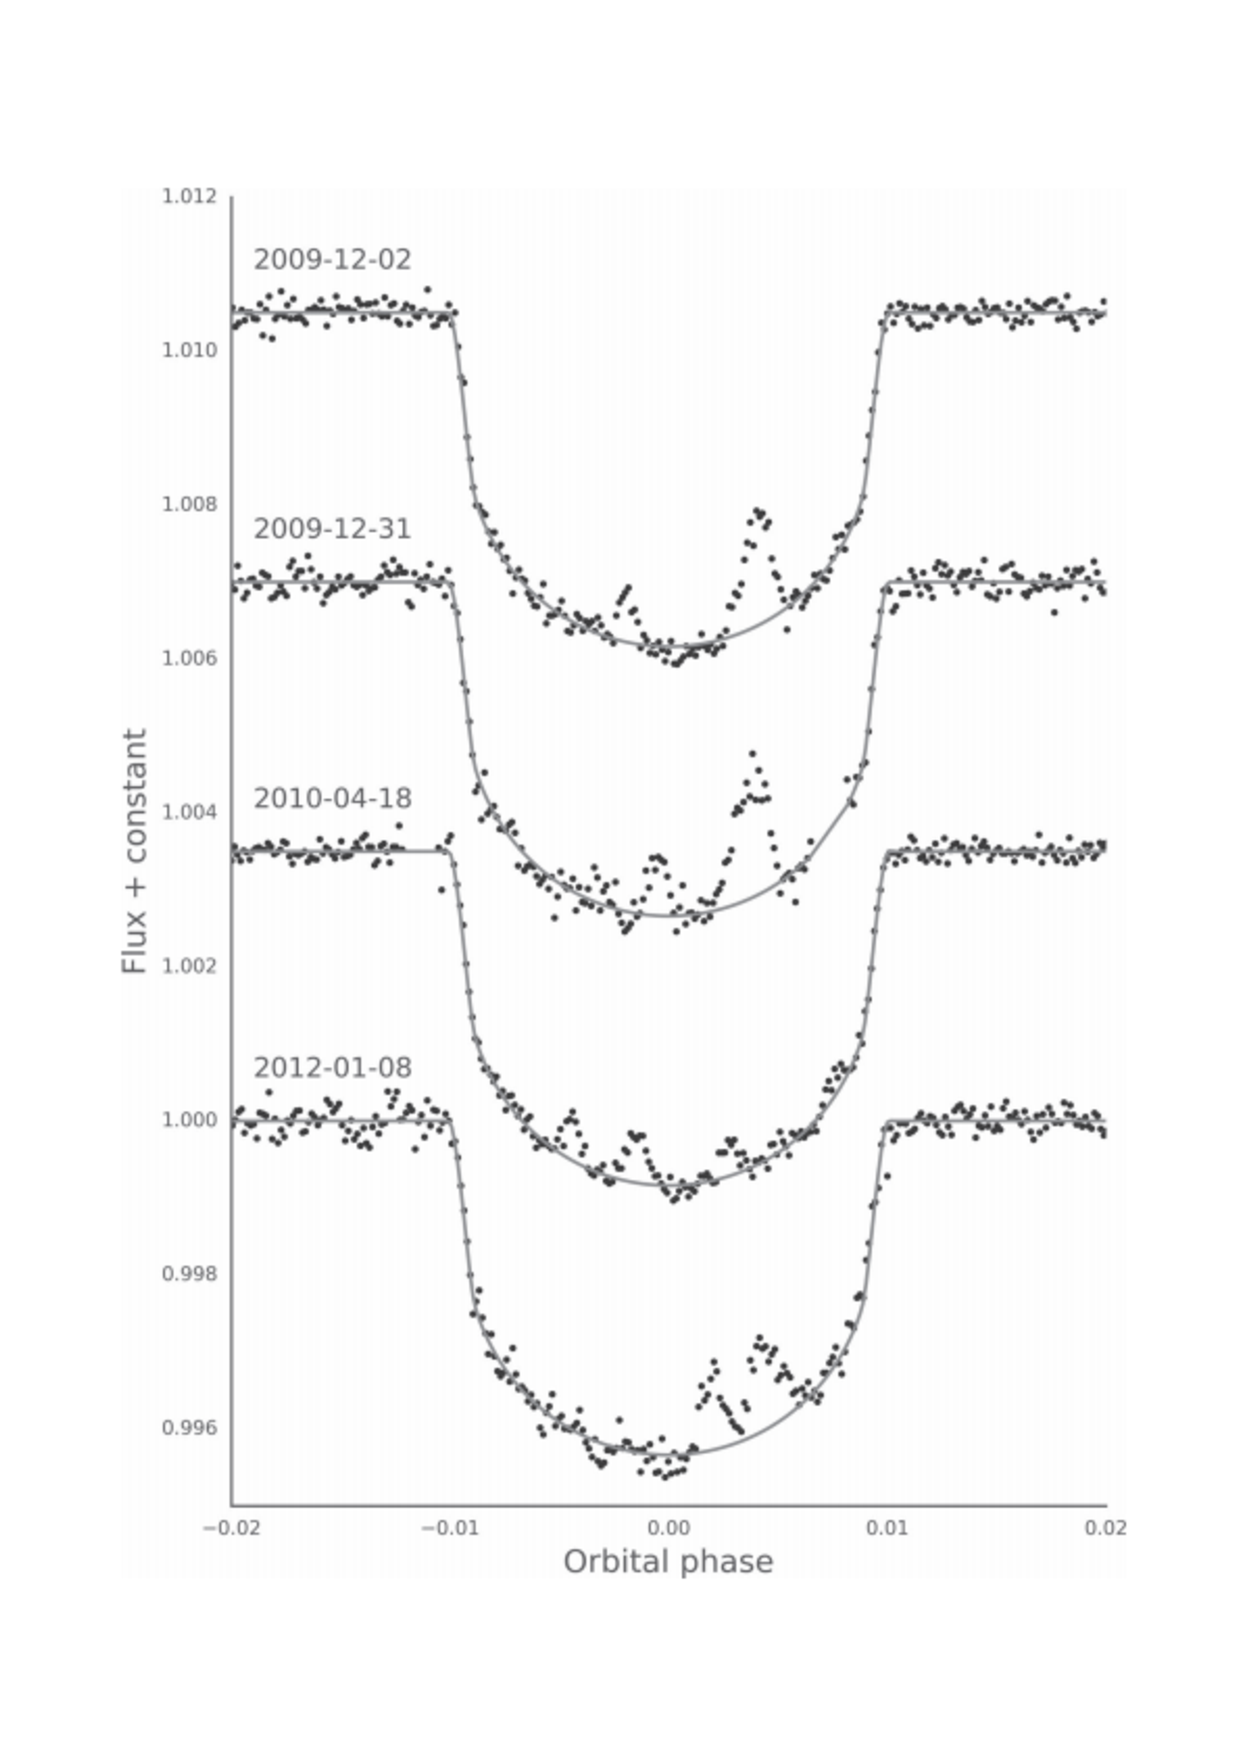
\includegraphics[scale=0.4]{Figures/1-Introduction/hatp_11_spots.pdf}
    \caption[Light curves with examples of starspot "bumps" in exoplanet transits]{Examples of \textit{Kepler} transit light curves for HAT-P-11 b. Data points are \textit{Kepler} fluxes and the curves indicate the best--fit transit model. Positive "bumps" in the light curve are due to the exoplanet passing in front of a starspot. Image credit: \citet{Morris_etal_2017}}
    \label{fig:spot_occultation_example}
\end{figure}

There are other techniques that can be used to observe starspots, such as Doppler imaging: however, this technique is limited to fast rotators since the Doppler shift caused by the starspot is proportional to the radial velocity. A much more common way of observing starspots on slower rotators is through spot occultations by transiting exoplanets. Transiting exoplanets pass in front of their host star and cause a small dip in the light curve of their host star. The transiting method has been the most successful way of discovering exoplanets since the launch of space telescopes such as \textit{Kepler}. During the transit of any object, the flux lost is proportional to the intensity of the area occulted. When an exoplanet transits a starspot, a cooler region of the stellar surface is occulted and causes a positive flux anomaly in the transit light curve as shown in Figure \ref{fig:spot_occultation_example}.

\subsection{Chromosphere}
\label{Chp1_atmosphere_chromosphere}
The chromosphere is the region that lies above the photosphere extending outward for approximately 2000~km. Awareness of the outer layers of the Sun's atmosphere started through observations during solar eclipses; it was only during these events that the light from the photosphere was obscured and the light from the chromosphere and corona could be revealed. The chromosphere is seen as a pink ring of emission at the solar limb and is only visible for a few seconds during an eclipse.

\begin{figure}
    \centering
    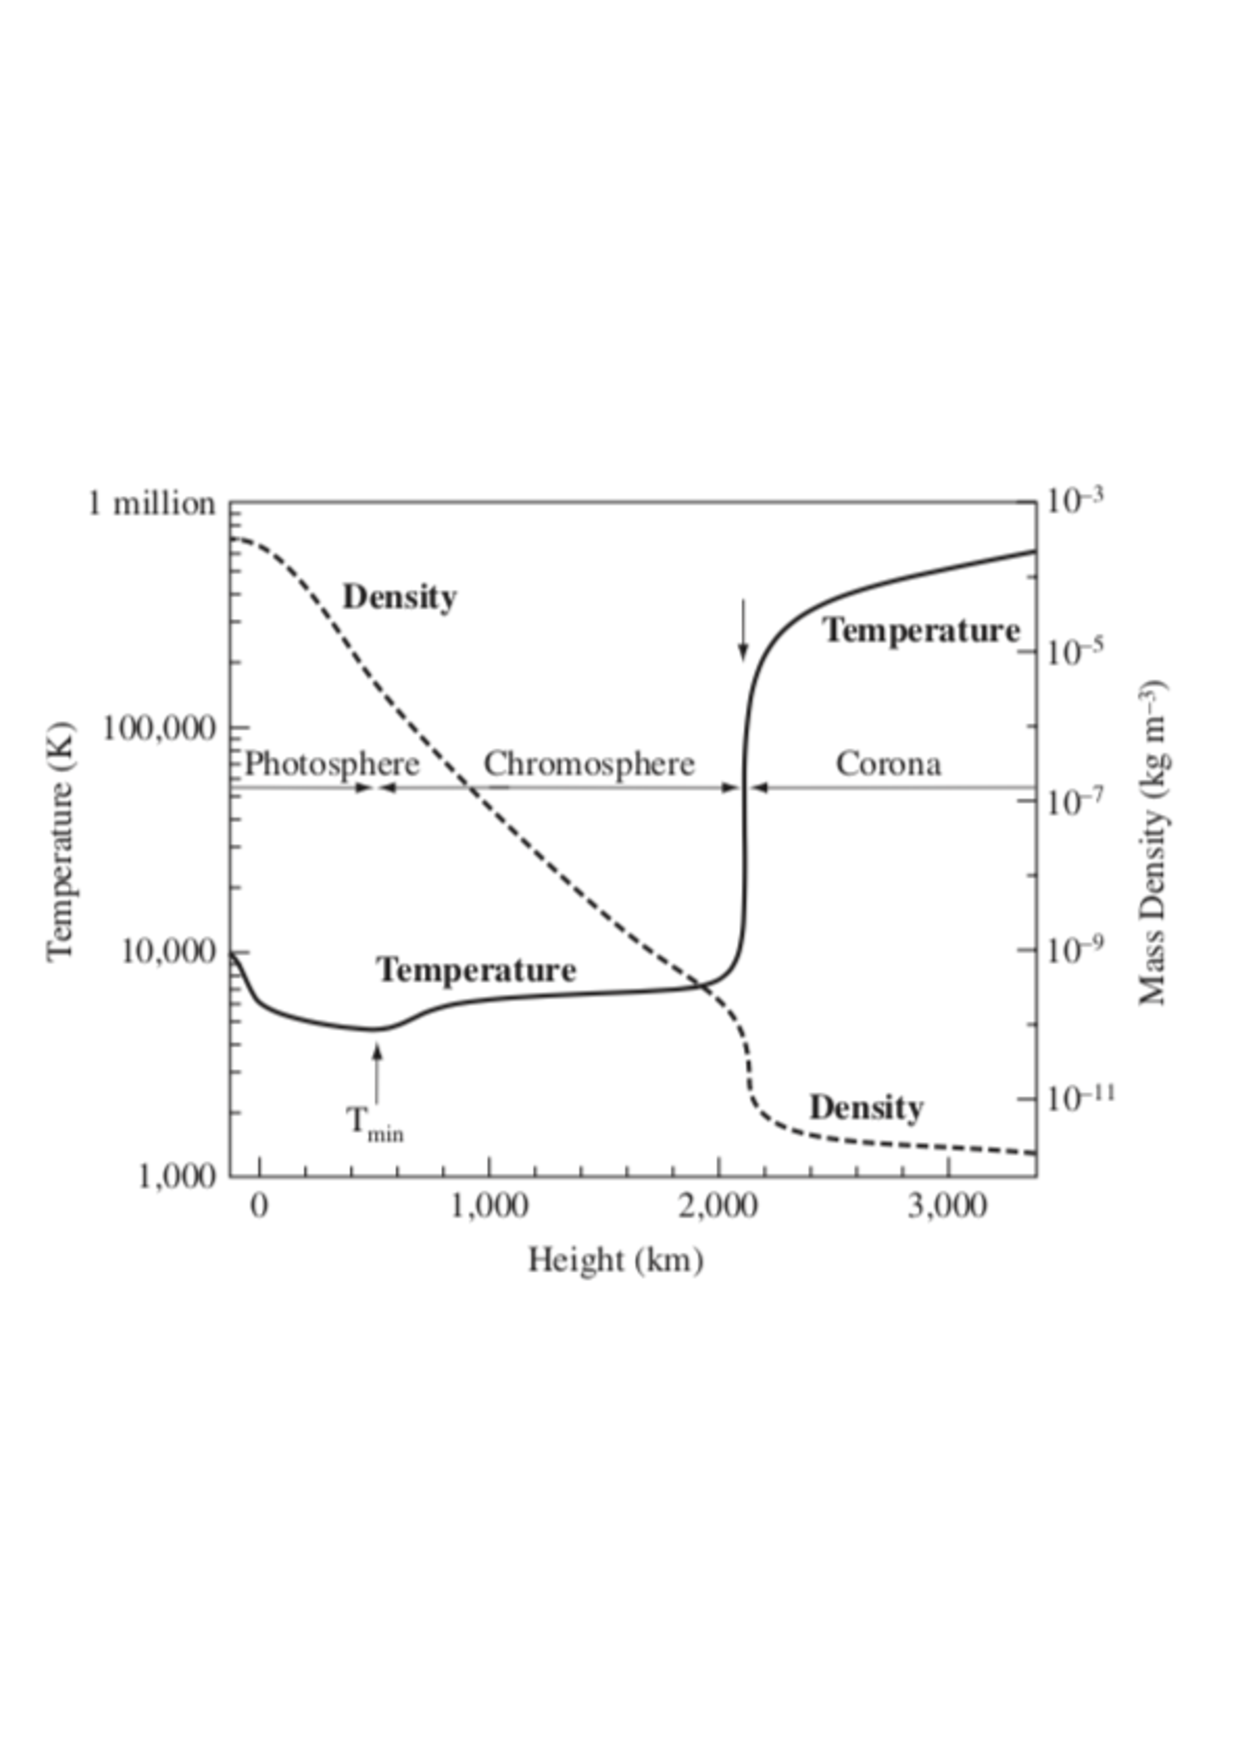
\includegraphics[scale=0.5]{Figures/1-Introduction/val_model_MHD_of_Sun_textbook.pdf}
    \caption[VAL model that shows the mean variation of temperature and density with height in the solar atmosphere]{Schematic of the mean variation of temperature and density with height in the solar atmosphere according to the VAL model. Image credit: \citet{Priest_2014_MHD_sun}}
    \label{fig:val_model}
\end{figure}

Early work on the spectra of both the chromosphere and corona showed there were numerous emission features of ionised species that could only be present due to high temperatures. The temperature rises from $\approx$ 4400 K in the photosphere to 7000 K in the chromosphere and rises even further to 1,000,000 K in the corona. This is clearly seen in Figure \ref{fig:val_model} which shows the mean variation of temperature and density with height in the solar atmosphere according to the VAL model (named after the scientists who developed the model). The VAL model \citep{Vernazza_etal_1981} is a semi-empirical 1-D model that successfully fits a number of spectral lines from different regions and well--represents the average properties of the Sun. The temperature rise seen in the chromosphere and corona cannot be explained by thermal processes alone, therefore there must be an additional heating mechanism at work. This is still an active topic of research, but the most likely theories are MHD wave heating and magnetic reconnection (for a more thorough review of the topic see e.g. \citealt{Parnell_DeMoortel_2012}). In any case, the heating in the outer layers of the star is inherently linked to the magnetic field of the star, and any emission from these layers can be used to probe the magnetic field.

Magnetic features that appear in the chromosphere include spicules \citep{Roberts_1945} and their larger counterpart macrospicules \citep{Bohlin_etal_1975}. These are tight jets of plasma that stream upward through the chromosphere. In addition to magnetic features that we can resolve on the Sun, since the chromosphere is heated by an additional magnetic process, we observe emission reversals in the cores of prominent Fraunhofer spectral lines such as \caII, an example of such emission is shown in Figure \ref{fig:Chp1_eg_Ca_emission}. The emission seen in the cores of these lines indicate that the source function ($S_{\upsilon}$) in the chromosphere is much larger than in the top of the photosphere. The source function is defined as the specific intensity emitted at a particular wavelength (or frequency) and is given by Equation \ref{Eq:source_function}, where $j_{\nu}$ is the emission coefficient and $k_{\nu}$ is the absorption coefficient.

\begin{equation}
    S_{\nu} = \frac{j_{\nu}}{k_{\nu}}
    \label{Eq:source_function}
\end{equation}

\begin{figure}
    \centering
    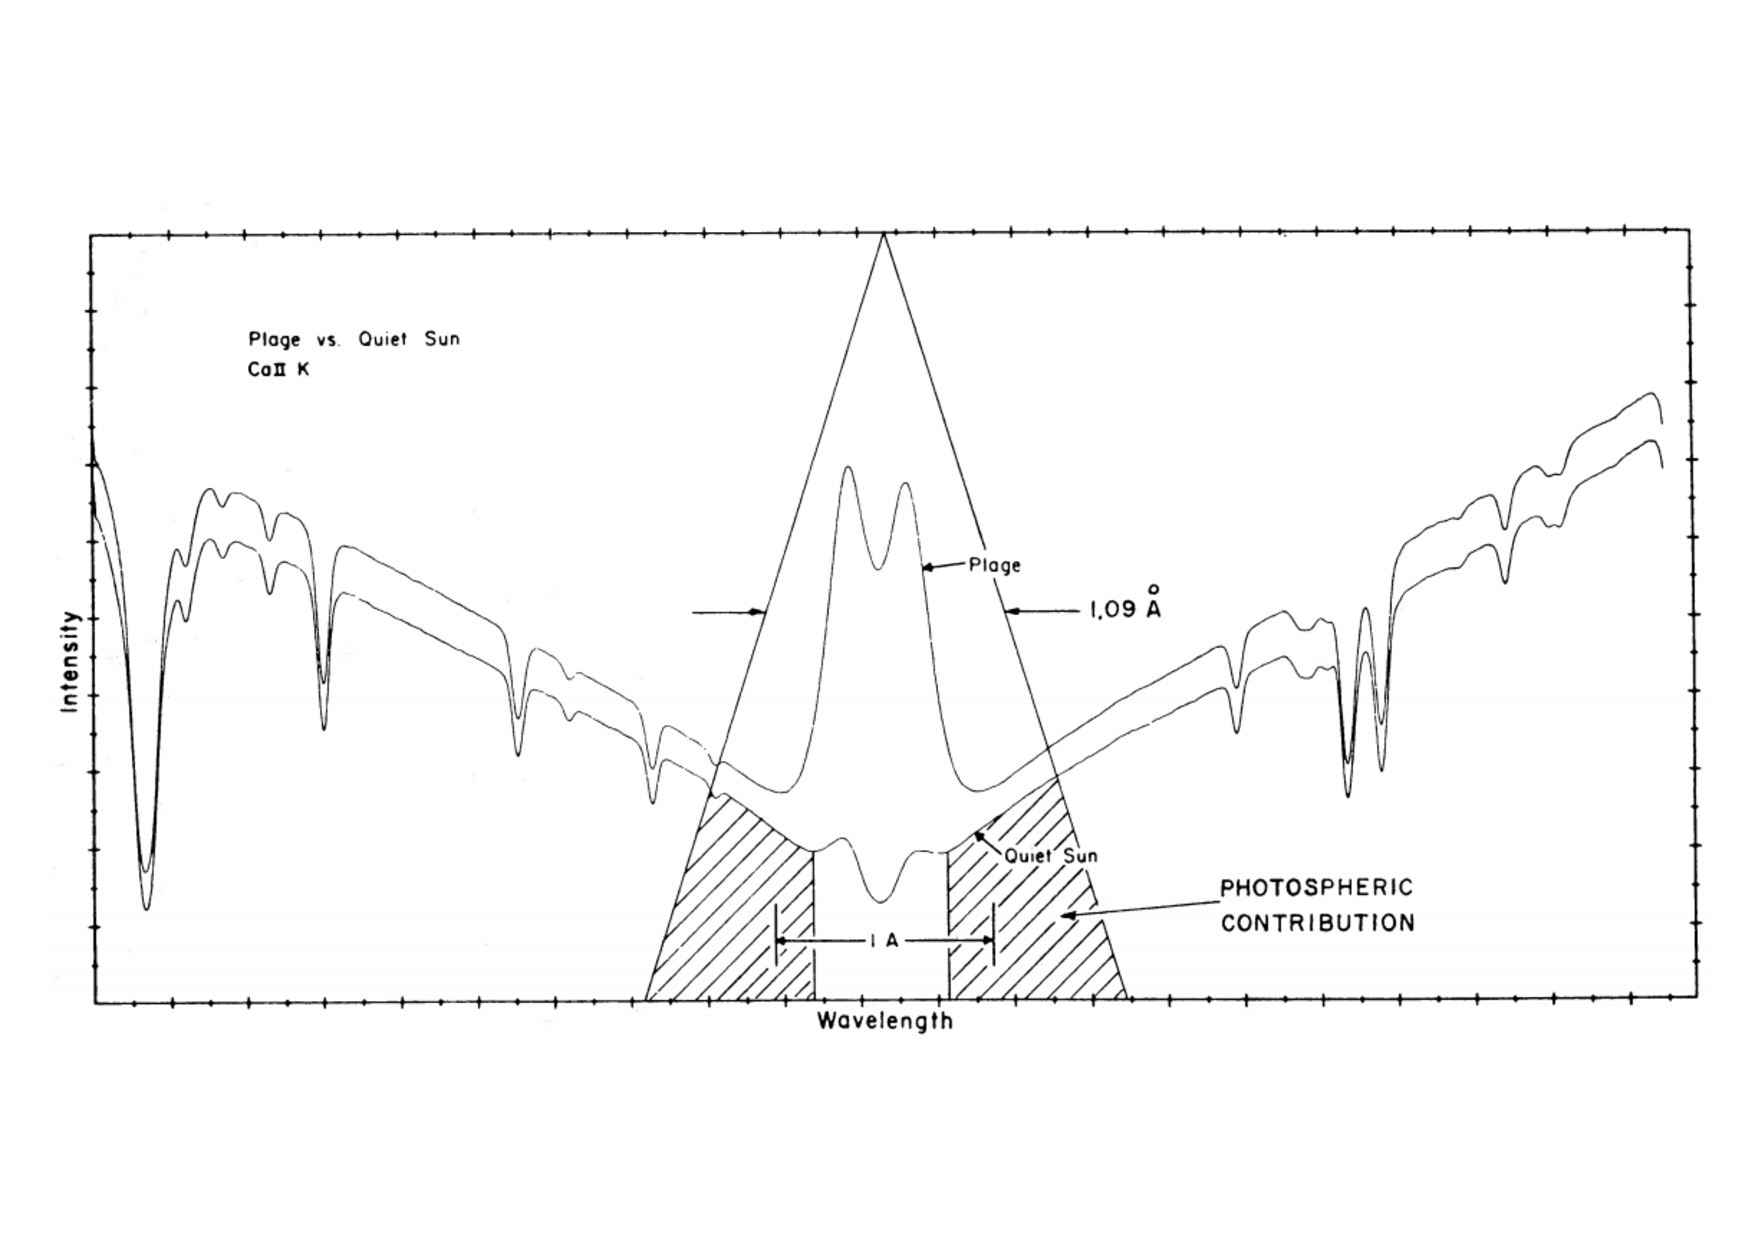
\includegraphics[width=0.9\textwidth]{Figures/1-Introduction/example_ca_emisison.pdf}
    \caption[Example of chromospheric emission in the Ca II K line]{Example of the centre of the Ca II K line with an active region of plage versus the quiet Sun. Image credit: \citet{Hartmann_etal_1984}}
    \label{fig:Chp1_eg_Ca_emission}
\end{figure}

The connection between chromospheric emission in the \caII lines and the magnetic field has been known since \citet{Leighton_1959} found that plage corresponded to areas of calcium emission on the Sun. Studies of the calcium emission over the solar cycle also shows that it has a measurable difference (e.g. \citealt{White_Livingston_1981}) in comparison to other parameters such as the solar irradiance. Another advantage of the emission from the \caII lines is that they are not sensitive to magnetic polarity, therefore they are a good proxy for the total unsigned magnetic field \citep{Linsky_Avrett_1970}. Additional spectral lines also show chromospheric emission, but the \caII spectral lines are by far the most commonly used.

The emission reversals in the \caII spectral lines (located at 3968.47 \AA \space and 3933.66 \AA \space respectively) vary linearly with the magnetic field strength \citep{Frazier_1970}. This provides a very useful tool to study the magnetic activity on other stars, as these spectral lines can be seen in spectroscopic observations. The \caII lines have been studied for decades on other stars, starting with the Mount Wilson Observatory (MWO) project founded by O. Wilson to try and find stellar cycles analogous to that of the Sun through the monitoring of the \caII lines \citep{Wilson_1968}.

This project went on to build a new more efficient instrument known as the HK Photometer 2 \citep{Vaughan_etal_1978} which led to the introduction of the now standard S index for measurement of calcium emission. The S index takes a measurement of the flux within the \caII lines and normalises it by the flux in two continuum reference channels as shown in Equation \ref{Eq:s_index}, where $N_{x}$ is the total counts in the relevant channel. Two 1.09 \AA \space wide triangular channels are centred on the \caII lines, while the R and V channels are 20 \AA \space wide centred on 40001.07 and 3901.07 \AA \space respectively. Generally, S indexes from other spectrographs are calibrated to the Mount Wilson S index (hereafter, \Smw) as the value of the S index is dependent on the resolution and throughput of the spectrograph.

\begin{equation}
    S = \frac{N_{H} + N_{K}}{N_{R} + N_{V}}
    \label{Eq:s_index}
\end{equation}

There are some issues with using the S index to compare the calcium emission from stars with differing spectral types. For stars at an equal distance, the values of $N_{R}$ and $N_{V}$ will be larger for more massive stars and smaller for less massive stars. In addition to this, the 1.09 \AA \space channel for the \caII lines is wide enough to admit light that comes from the photosphere as well as the chromospheric component. This introduces a colour or mass dependency into the S index and therefore cannot be used to compare emission of stars with varying spectral types.

This colour/mass dependency was resolved by \citet{Noyes_etal_1984} who developed the chromospheric ratio \Rprime, defined by Equation \ref{Eq:Rprime}: $\mathcal{F}$ represents the absolute flux in the H and K channels from chromospheric emission and $\sigma T_{eff}^{4}$ is the bolometric flux. It is custom to present the \Rprime indicator in terms of $\log(R^{'}_{HK})$ due to the small values typically seen. Since the absolute fluxes are more difficult to calculate, \citet{Middelkoop_1982} determined an empirical relationship between the S index and the absolute fluxes known as $R_{HK}$. \citet{Noyes_etal_1984} improved upon this relation by determining the photospheric contribution ($R_{phot}$) as a function of $B-V$ colour and subtracting this from $R_{HK}$ to obtain $R^{'}_{HK}$ -- a measure of the chromospheric contribution.

\begin{equation}
    R^{'}_{HK} \equiv \frac{(\mathcal{F}_{H} + \mathcal{F}_{K})_{Chromo}}{\sigma T_{eff}^{4}} = R_{HK} - R_{phot}
    \label{Eq:Rprime}
\end{equation}

In order to calculate the \Rprime indicator from the \Smw, firstly Equation \ref{Eq:rhk} is used to convert the \Smw value into an $R_{HK}$ value, where $C_{cf}$ is the correction factor and is a function of the $(B-V)$ colour of the star as shown in Equation \ref{Eq:c_cf}. The photospheric contribution to the \caII spectral lines ($R_{phot}$) has also been calibrated as a function of $(B-V)$ colour of the star and is calculated by Equation \ref{Eq:rphot}.

\begin{equation}
    R_{HK} = 1.34{\times}10^{4}C_{cf}S_{MW}
    \label{Eq:rhk}
\end{equation}

\begin{equation}
    \log C_{cf} = 1.13(B - V)^{3} - 3.91(B-V)^{2} + 2.84(B-V) - 0.47
    \label{Eq:c_cf}
\end{equation}

\begin{equation}
    \log R_{phot} = -4.898 + 1.918(B-V)^{2} - 2.893(B-V)^{3}
    \label{Eq:rphot}
\end{equation}

One parameter that is not considered in the \Rprime indicator is metallicity, which will affect the depth of the convection zone within the star. The metallicity will change the interior opacity of the star, which then changes the point at which the convection zone starts. Metal-rich stars will have a deeper convection zone and thus have a longer convective turnover time ($\tau_{C}$). This also affects the shape of the \caII line profiles: metal-poor stars have shallower line profiles which mimic high levels of chromospheric activity making the star appear more active and younger than metal-rich stars \citep{Rocha-Pinto_Maciel_1998}.

Other spectral lines also include a chromospheric component, including the \Halpha line (located at 6562.81 \AA). This is commonly used in studies of low-mass stars such as M dwarfs (e.g. \citealt{Newton_etal_2017}). This is due to the low level of continuum in the \caII region which makes calculation of the \Rprime indicator more difficult. Extensive research has been undertaken to investigate the correlation between \caII and \Halpha emission. A single one--to--one relationship does not exist between the two activity indicators and a wide variety of correlations have been found in other stars, as seen in \citet{Cincunegui_etal_2007}. The large variation in correlation can be explained by how plage and filaments contribute to the \caII and \Halpha lines, as suggested by \citet{Meunier_Delfosse_2009}.

\subsection{Corona}
The outermost layer of the solar atmosphere is the corona: a region of very hot, low density gas. The first indirect evidence of the corona came from optical spectral lines of highly ionised elements \citep{Grotrian_1939} which indicated that these elements originated from a region with very high temperatures. The majority of the radiation emitted from the corona is in the extreme ultraviolet and X-ray regimes, this makes detailed analysis of the corona difficult from the ground. It was not until the space age and the invention of rockets that images of the Sun in these wavelengths could be taken (e.g. \citealt{van_Speybroeck_etal_1970}).


\begin{figure}
    \centering
    \includegraphics[scale=0.45]{Figures/1-Introduction/cor_hole_combo.pdf}
    \caption[UV image of Sun showing coronal features]{Image of the Sun in three different ultraviolet wavelengths from NASA's Solar Dynamics Observatory in January 2014. A large coronal hole that spans from the south polar region to mid latitudes is seen alongside several active regions that show coronal loops. Image credit: NASA/SDO and the AIA, EVE, and HMI science teams.}
    \label{fig:corona_structure}
\end{figure}

There are several key structures that appear in the corona: these include coronal holes, coronal loops and X-ray bright points. Coronal holes were first studied by \citet{Waldmeier_1956} but high-detailed images of them were not available until the 1970's \citep{Huber_etal_1974}. Coronal holes are the darkest and least active region of the Sun and are associated with open field lines and the acceleration of the solar-wind. Coronal holes are also some of the most long-lived features on the Sun as near solar minimum, large coronal holes cover the north and south polar caps and can last for 7-8 years; shorter-lived coronal holes can also appear at lower latitudes during solar minimum. Coronal loops are closed magnetic loops that are connected to photospheric bipolar regions. X-ray bright points are small yet intense features that are scattered around the whole disc. Examples of some of these features are seen in Figure \ref{fig:corona_structure} in ultraviolet wavelengths from NASA's SDO.

The corona also shows magnetic activity features such as flares and coronal mass ejections (CMEs). Flares occur as a result of a relaxation in the magnetic field structure thus releasing magnetic energy that is radiated across the entire electromagnetic spectrum. CMEs are large scale plasma bubbles that expand out from the Sun and cause major modifications in the large-scale structure of the corona. CMEs are usually associated with other indicators of activity such as flares but they do not necessarily occur together: generally, weaker CMEs occur without any flare-like manifestation, but powerful flares do have associated CMEs \citep{Andrews_2003}. The frequency of CMEs depends on the phase of the solar cycle (as do other magnetic activity indicators); near solar maximum there can be up to 3.5 events per day, while near solar minimum they can occur once every 5 days \citep{Carroll_Ostlie_2006}. In addition to the magnetic features, the overall X-ray flux that is emitted from the corona is a good indicator of magnetic activity since the corona is heated via magnetic fields. X-ray emission shows a good correlation with chromospheric indicators and the magnetic flux density (e.g. \citealt{Schrijver_etal_1992,Pevtsov_etal_2003}) thus making it a useful tool to study magnetic activity on other stars.

The age of stellar X-ray astronomy began in the 1970's with the detection of Capella (a G-type giant star) as the first stellar coronal X-ray source \citep{Catura_etal_1975}. The first main sequence star to be detected in X-rays was Alpha Centauri \citep{Nugent_Garmire_1978}, which was identified as an inactive coronal source similar to our own Sun. The field was revolutionised when the Einstein telescope was launched in 1978 and made several key insights in stellar X-ray astronomy. Firstly, stars became one of the most prominent classes of cosmic X-ray sources as seen in \citet{Vaiana_etal_1981}; stars from the pre-main sequence, along the entire main sequence, and even giant stars were detected in the X-ray regime. The X-ray luminosity and distribution along the main sequence could not be in agreement with the long--favoured acoustic wave heating model for coronal heating. Coronal X-ray emission was now interpreted as an effect of magnetic coronal heating. Lastly, stars that are otherwise similar showed large difference in X-ray luminosity if their rotation periods were different \citep{Pallavicini_etal_1981}. Since then many surveys of stellar coronae have been undertaken using X-ray telescopes (e.g. \citealt{Fleming_etal_1995,Schmitt_1997,Nebot_etal_2013,Wood_etal_2018}). Even in the early surveys, the sensitivity was sufficient enough to suggest a lower limit to the main sequence X-ray luminosity of a few times $10^{25}$ ergs $s^{-1}$, similar to that of solar coronal holes.

The first X-ray spectrum of a stellar corona was obtained of Capella by \citet{Cash_etal_1978}, who correctly interpreted that the excess emission between 0.65 and 1 keV was due to a blend of highly ionised iron lines -- an iron complex. Another element of modern coronal X-ray astronomy was introduced by \citet{Walter_etal_1978} when they realised that sub-solar abundances were needed to fit the coronal X-ray spectrum. Now with the introduction of Chandra and XMM-Newton telescopes, a new era in X-ray astronomy has begun with the technology needed to perform high-resolution spectral studies.

It is worth noting that while X-ray observations are more resource--intensive (typically taken on the timescale of ks), they provide a direct link to the magnetic heating that causes the emission. X-ray luminosity does not have any strong dependencies on other parameters such as metallicity, thus making it a much more direct measure of magnetic activity. However, it is worth noting that during the solar cycle, the Sun's X-ray luminosity can be an order of magnitude higher or lower than the mean value.


\section{Ages of stars}
\label{Section:intro_ages}
Knowledge of stellar ages are useful in many different areas of astrophysics. For very young stars (i.e. $<$ 100 Myr), if we want to understand the timescale of planet formation then we must determine the stellar age. If we observe enough systems with various stages of planet formation, then this information can be fed back into theoretical models. In terms of galactic history, it is paramount that we can assign stellar ages for individual stars to understand the formation of the galaxy. This is particularly true when considering low--mass stars that are able to live long enough to be present for all epochs of star formation. Another example of how stellar age is an important parameter can be seen when considering the evolution of the Sun (both in the past and future): to fully understand the Sun, we must look at other solar-like stars at different stages in their evolution. These type of studies will give us greater insight into what conditions were like when life was forming on Earth and how the Sun will evolve in the future. When considering exoplanet systems, in order to deepen our knowledge of the dynamics of such systems or the potential migration that has taken place (in the case of hot Jupiters) we need to know the age of the star. Stellar ages are particularly important when it comes to the search for life outside of our own solar system as they will help us understand the timescale needed for such biological evolution. These are just a few of the many reasons why stellar ages are important in astrophysics: so how do we calculate these ages?

The Vogt-Russel theorem states that the structure of the star can be uniquely determined by its mass and chemical composition; other factors may play a role (such as rotation, magnetic field or companions) but mass and composition dominate. The age of a star can influence the state of the star as over time the chemical composition of the star will change: however, this is due to nuclear fusion taking place in the star, and the stellar age is not the direct agent of this change. Consequently, we cannot directly measure a star's age, but rather it must be estimated or inferred. The only accurate and precise stellar age known is for our own Sun, but this value is not calculated from observing the Sun but rather through the study of meteorites. Meteorites are portions of asteroids or comets that have fallen to Earth, containing long-lived radioactive isotopes of elements that can be used to age the material. Since meteorites are portions of asteroids and comets that are the left over debris from the planet formation process, it follows that they should have the same age as the solar system and the Sun. The age of the Sun is found to be $4.57 \pm 0.02$ Gyr, where 1 Gyr is equivalent to a billion years \citep{Bahcall_etal_1995}. This is known as a fundamental age, as the physical process behind the method is fully understood. In this following sections I will describe some common methods used to determine the ages of stars, and in particular the ages of single stars that are on the main sequence, as these are the main focus of the work presented in this thesis. For a more thorough review of different methods to determine ages of stars see \citet{Soderblom_2010}.

\subsection{Semi-fundamental ages}
While the only fundamental age known is for our own Sun, there are some methods that produce semi-fundamental ages i.e. methods where the physical process is understood but must invoke a few (well-founded) assumptions. One of these is known as nucleocosmochronometry and uses the presence of long-lived isotopes in stellar spectra to date the stars. Typically the isotopes used are $^{238}$U and $^{232}$Th which have half-lives of 4.47 and 14.05 Gyr respectively. However, these spectral lines can only be measured in metal-poor stars where the weak isotope lines can be measured within the presence of other line blends. Therefore, the method is used to date the oldest and therefore metal--poor stars that formed at the earliest epoch in the galaxy. While the physical process that underlies this method (i.e. nuclear decay) is well known, the initial abundance of the isotope within the star is an unknown quantity, thus making the age a semi-fundamental value. The initial abundance of the isotope is scaled from other r--process elements. These r-process elements are all heavier than iron and are created in the aftermath of core--collapse supernovae or binary neutron star mergers. The abundance of these r--process elements are measured and by assuming production rates for these elements, allows the initial abundance of the isotope to be estimated. \citet{Ludwig_etal_2010} quantified the uncertainties associated with this age-dating method and found that the accuracy is poor when considering a single star -- uncertainties of $\approx$ 2 Gyr are common when considering observation uncertainties only. Improved results should come from larger samples of stars (e.g. globular clusters or dwarf galaxies) where a larger sample of old, metal poor stars are found (see e.g. \citealt{Hansen_etal_2018}). 

Another semi-fundamental age dating method uses kinematics. In this method the motion of a group of stars is traced into the past, determining when they were in closest proximity to each other: this is then assumed to be the time of formation. While this method is independent of any stellar physics as it relies mainly on astrometry, it requires high-quality kinematics data in all three dimensions, including parallax and radial velocities. In addition to the full 3-D kinematic data, good accuracy is needed, therefore this method is predominately used for nearby groups (see e.g. \citealt{Makarov_2007}). Typically, using kinematic data, we cannot go back further than 20 - 30 Myr due to the uncertainties in the input parameters. Also, some young groups appear to have very little net expansion \citep{Mamajek_2005} therefore the time at which the group of stars was closest together is ill-defined. Additionally, a fundamental limitation on this method is the evolution of galactic orbits over time. As stars and clusters orbit about the galaxy, they encounter massive objects that can disrupt their orbits and create field stars, for example. The timescale for such interactions with these objects is $\approx$ 200 Myr \citep{Janes_Phelps_1994} which is similar to the galactic rotation period. Therefore, only young stars can be dated using this method, as it can be assumed that their galactic orbits are undisturbed.

\subsection{Model dependent ages}
As discussed in the previous section, there are some methods that can determine semi-fundamental ages but can only be applied to a limited number of stars. Consequently, in order to determine ages for other stars, methods must be used that are based on stellar models.

\subsubsection{Isochrones}
One such model--dependent method is the use of isochrones on a Hertzsprung-Russell Diagram (HRD). A HRD plots the absolute magnitude as a function of stellar temperature (or observable equivalent) and shows the various stages of a star's evolution depending on the position within the diagram. The main sequence on the HRD goes from the top left to the bottom right of the diagram and shows the stars while they are in their hydrogen--burning phase (i.e. nuclear fusion of hydrogen into helium is occurring within the core). As the star evolves and uses up the hydrogen supply within the core, they move to the right on the HRD, becoming subgiants and eventually giants. However, the age at which stars evolve off the main sequence is dependent on the mass of the star -- more massive stars use up their hydrogen supply quicker than low mass stars. An isochrone is defined as a line on a diagram connecting points to the same time; in the stellar case, this represents a population of stars of varying masses with the same age. Therefore, an isochrone with a particular age will show the main sequence turn off at a different stellar mass. Comparing isochrones with varying ages to cluster data (as shown in Figure \ref{fig:OC_isochrone_example}) allows the main sequence turn off to be determined. If the masses of the stars that have evolved off the main sequence are known, then stellar models can be used to determine the age of the cluster. This technique has been successfully used to date open clusters, as we can observe the full population of stars with the same age.

\begin{figure}
    \centering
    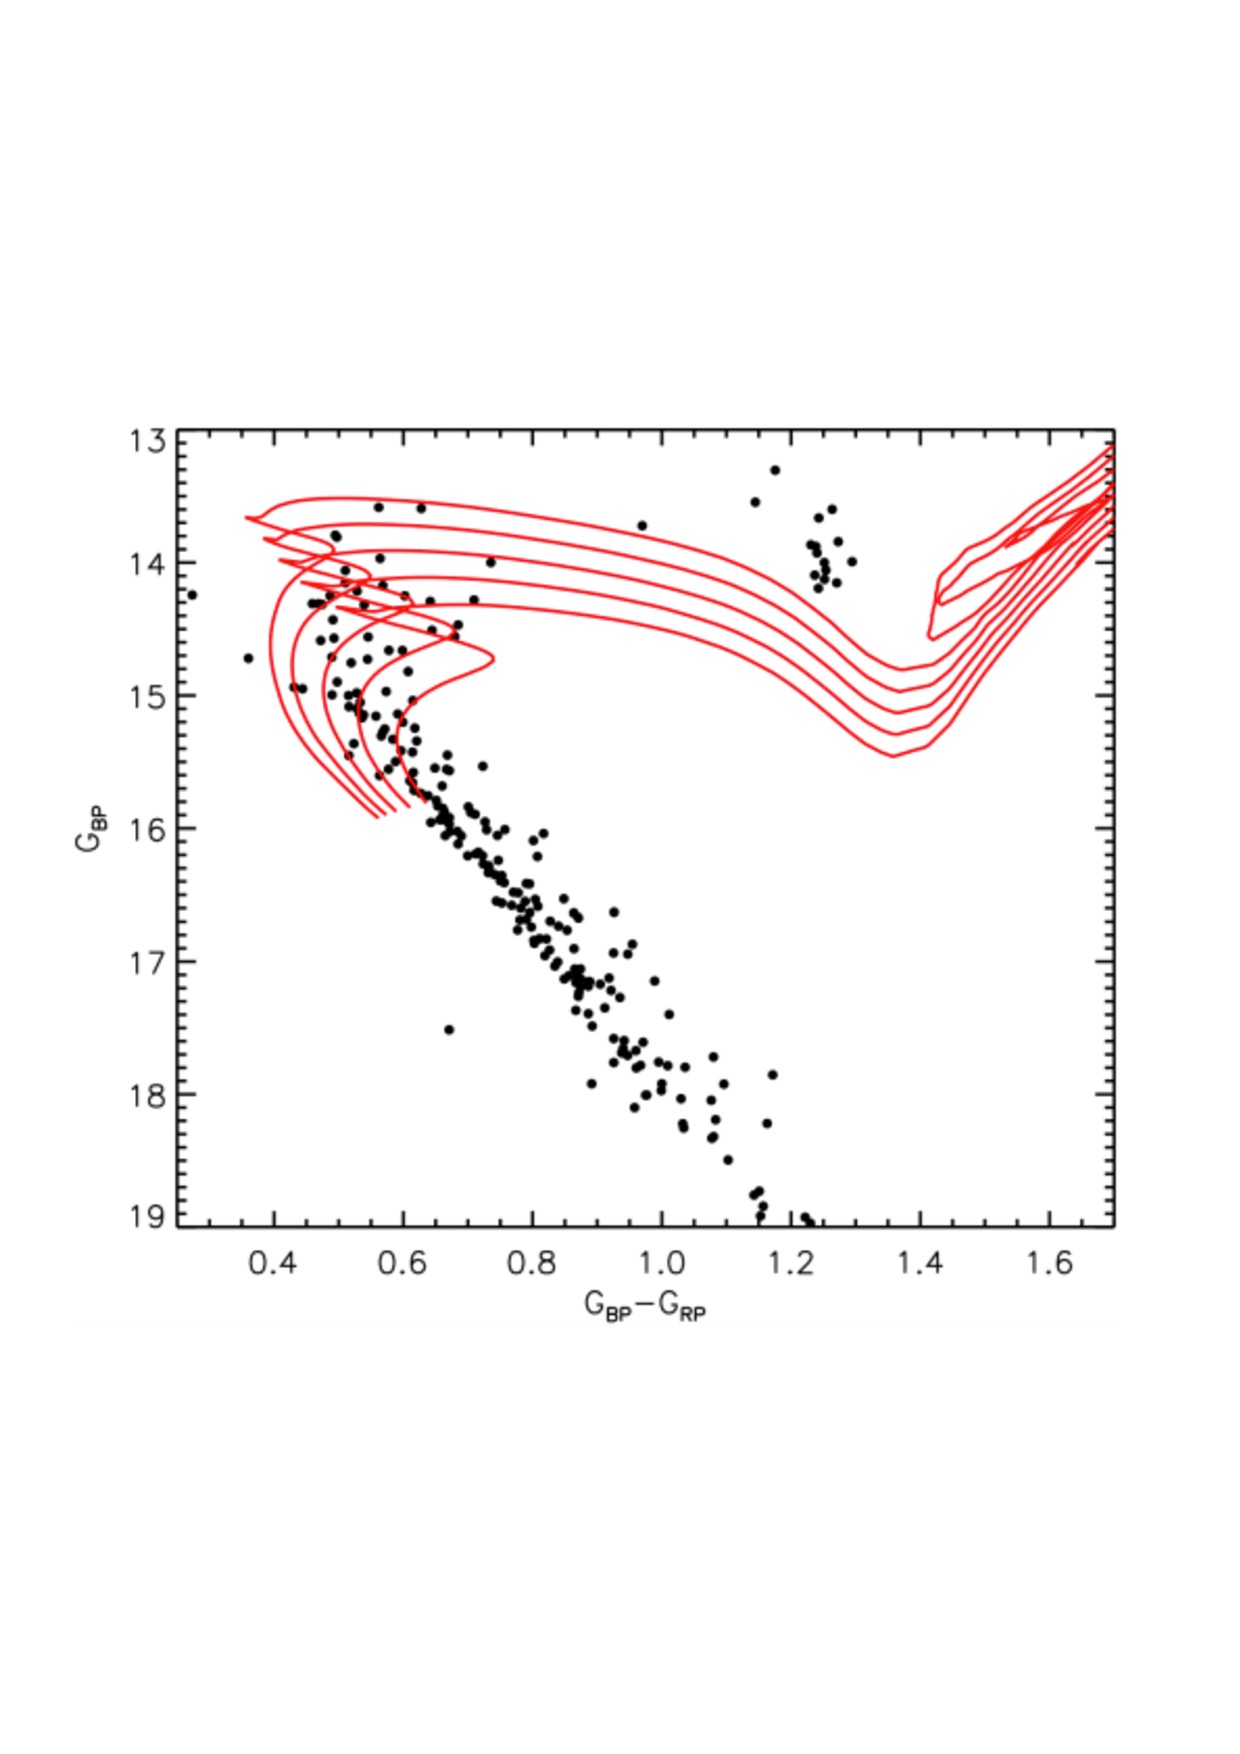
\includegraphics[scale=0.45]{Figures/1-Introduction/gaia_OC_example.pdf}
    \caption[Example of model isochrones for a cluster]{Example of a colour-magnitude diagram (observational equivalent of HRD) for NGC 2818 as seen in \textit{GAIA} filters. Red lines indicate isochrones with ages between $log$ t = 8.85...9.05 (in steps of 0.05). Image credit: \citet{Bastian_etal_2018}}
    \label{fig:OC_isochrone_example}
\end{figure}

Isochrones have also been used to determine ages of single field stars. However, since a distributed fit is not possible (as with the cluster data), a different method must be used to analyse the data. Isochrones have complex shapes, particularly near the main sequence turn--off, and multiple isochrones may pass through the same point on the HRD. This creates a degeneracy when trying to determine the ages of field stars, since only one data point exists. Some of this degeneracy can be removed when either the abundances are known or if the star is in a binary system.

In order to calculate an age for a field star using the isochrone method, the best estimate of the temperature, metallicity and luminosity (along with uncertainties) must be known in order to minimise the degeneracy. One method is to interpolate among model isochrones to the location of the star in the HRD: yet this method introduces bias because of the complex shapes of the isochrone and the non-uniform spacing between the isochrones. The majority of stars should fall near the ZAMS but uneven spacing in isochrones results in biases towards older ages. This bias is clearly seen in one of the earliest attempts using this method \citep{Perrin_etal_1977} as most of the ages were found to be greater than 10 Gyr. In recent years, more sophisticated methods (such as Bayesian methods) have been applied  to reduce the effect of these biases (e.g. \citealt{Takeda_etal_2007}). However, errors typically have values between 20\% - 50\% before taking into account any systematics.

\subsubsection{White dwarf cooling}
\label{Chp1_WD_cooling_age_method}
An alternative method uses the presence of white dwarfs to age stars in a cluster and/or a binary system. White dwarfs are the final remnant cores of low and intermediate stars after they have used up their hydrogen supply within the core and completed their evolution as giant stars. White dwarfs are highly dense objects with typical masses of 0.6 M$_{\odot}$ with radii comparable to the earth ($\approx$ 7000 km) \citep{Madej_etal_2004} and made up predominantly of product elements from helium fusion -- carbon and nitrogen. They are particularly important astronomical objects to study as they are representative of the stellar population as a whole: the majority of stars will become white dwarfs.

Since white dwarfs are the remnant cores of stars they no longer undergo nuclear fusion. Instead, they are powered by the internal energy stored in the thermal motions of the constituent ions and gradually cool over time \citep{Mestel_1952} resulting in observable changes in luminosity and temperature. We can therefore deduce a white dwarf isochrone, but to determine the ages of these white dwarfs more knowledge is needed in comparison with the usual isochrone discussed previously. The white dwarf cooling models are relatively well understood and can inform us of the time that it has taken for the white dwarf to cool to a particular temperature, but this only pertains to the white dwarf portion of the stellar life. In order to obtain the age of the white dwarf, information is needed about the progenitor star. This is usually obtained through an initial-final mass relationship (IFMR). This relationship links the mass of the white dwarf to the initial mass of the star prior to mass loss on the asymptotic giant branch and relies on stellar models. In order to calculate the mass of a white dwarf, spectroscopic observations are needed to calculate the effective temperature and surface gravity (log(g)). Once the mass of the white dwarf is known then one can use the IFMR to infer the mass of the progenitor star. Lastly, stellar evolution code can provide the main sequence lifetime of the progenitor star given its mass, which can be added to the white dwarf cooling time to obtain the age of the white dwarf.

This technique has been used to determine ages for clusters, particularly globular clusters, in recent years (e.g. \citealt{Torres_etal_2015}) giving us insight into the true ages of the oldest stars in our galaxy. It is particularly useful to compare the ages determined from white dwarfs to those from main sequence turn--off ages in clusters, as seen in \citet{Garcia-Berro_etal_2010}. This study's motivation was to try and explain the discrepancy between the ages from the two methods by adding a predicted theoretical mechanism (crystallisation of a product of helium burning) which would delay the cooling phase of a white dwarf. As predicted, by adding in this mechanism the age discrepancy was resolved. Even clusters that have generally accepted ages like the Hyades are being studied using white dwarfs \citep{Salaris_Bedin_2018}. This technique has also been used to age stars in binary systems with a white dwarf companion (e.g. \citealt{Liebert_etal_2013}) and even the galactic halo \citep{Kilic_etal_2019}. It is the use of the method in these environments outside of clusters where no other age dating method could be invoked that makes this such a useful tool if a white dwarf is present.

\subsubsection{Asteroseismology}
Asteroseismology is the study of stellar oscillations in order to gain insight into the interior layers of a star. It is particularly useful for determining fundamental parameters of a star such as mass, effective temperature, log(g) and even age. In the context of stellar ages, it has been revolutionary for determining ages of isolated, old main sequence field stars. The stellar oscillations are caused by waves within the interior of the star interfering with one another to generate standing waves. There are two types of oscillations, defined by the restoring force that acts upon them: gravity (g) modes where buoyancy is the restoring force, and pressure (p) modes where gradients of pressure act as the restoring force. The main advantage of studying asteroseismology is that since the oscillations originate from within the interior of the star, they allow information about this area to be obtained.

In the early 1960's, the discovery and interpretation of solar oscillations led to the development of the helioseismology field (for a review see \citealt{Christensen-Dalsgaard_2002}). In the Sun, we see p--modes that are  driven stochastically but are intrinsically stable, created by turbulent motions in the sub-surface convection zone \citep{Samadi_Goupil_2001}. These oscillations are relatively high frequency -- in the range of 1000 - 5000 $\mu$Hz which corresponds to 3 -- 17 minute periods. These types of oscillations are generally referred to as solar-like oscillations: however they can occur in non-solar-like stars (such as giant stars), as the stars simply need to be cool enough to have an outer convection zone. Gravity or g--modes are generally found in other stars such as white dwarfs and stars that pulsate, such as some B stars. Since these modes are generated deep within the core, they are strongly dampened by convective motion and are typically not seen in solar-like stars: thus the rest of this section will concentrate on p--mode oscillations.

The geometrical structure of oscillation modes are described as a spherical harmonic which assumes spherical symmetry in stars. There are three important integers to consider: Firstly, $n$, which is the radial order and specifies the number of nodal shells in the standing wave. Secondly, $l$, which measures the total number of nodal lines on the surface. Modes with a value of $l=0$ are known as radial modes and $l$ values greater than this are known as non-radial modes. Since the surfaces of stars are not resolved, typically only modes with values of $l$ less than four are observable. The third integer is $m$, the azimuthal order, and has values from $+l$ to $-l$. The oscillation frequency does not depend on $m$ unless spherical symmetry is broken, for example in the presence of a magnetic field or if the star is rotating. Therefore, for a rotating star with a mode with given $n$ and $l$ values, there will be a split in the frequency of the mode into a multiplet with $2l + 1$ components (one for each value of $m$). It is possible to determine the rotational frequency of a star as it is proportional to the frequency separation between these components. However, high quality data is needed as the typical frequency separation between components is typically a few $\mu$Hz.

Space missions such as \textit{CoRoT} and \textit{Kepler} have revolutionised the asteroseismology field with exquisite precision light curves and long timescales. For example, one of the early surveys for asteroseismology with Kepler by \citet{Chaplin_etal_2011} looked at over 2,000 main sequence and giant stars in short cadence mode and detected solar-like oscillations for approximately 500 stars. Fourier analysis is performed on the Kepler light curves to obtain a power spectrum that contains information on the frequencies of any oscillations present. Figure \ref{fig:power_spectrum_example_sun} shows an example for the Sun: panel (a) shows the full power spectrum and panel (b) shows an zoomed in portion with labelled modes and frequency separations. From the power spectrum we can define some variables that are key in asteroseismology studies; in panel (a) we see that the peak heights create an envelope which can be used to define $\nu_{max}$ -- the frequency of maximum power -- which has a value of 3,100 $\mu$Hz for the Sun. The next parameter that can be defined is $\Delta \nu$, the large frequency separation, which is define as the spacing between consecutive radial overtones (i.e. modes with a given $l$ whose $n$ values differ by one). The large frequency separation has a value of 135 $\mu$Hz in the Sun. The last parameter that can be calculated is the small frequency separations (e.g. $\delta \nu_{0,2}$); these are frequency separations between close pairs with a difference of two in $l$ value and difference of one in $n$ value as shown in panel (b) of Figure \ref{fig:power_spectrum_example_sun}. An additional small frequency separation can be defined ($\delta \nu_{0,1}$) as the $l=1$ modes do not fall exactly half way between the $l=0$ modes. Therefore, $\delta \nu_{0,1}$ is the amount by which the $l=1$ mode are offset from the midpoint of the $l=0$ modes.

\begin{figure}
    \centering
    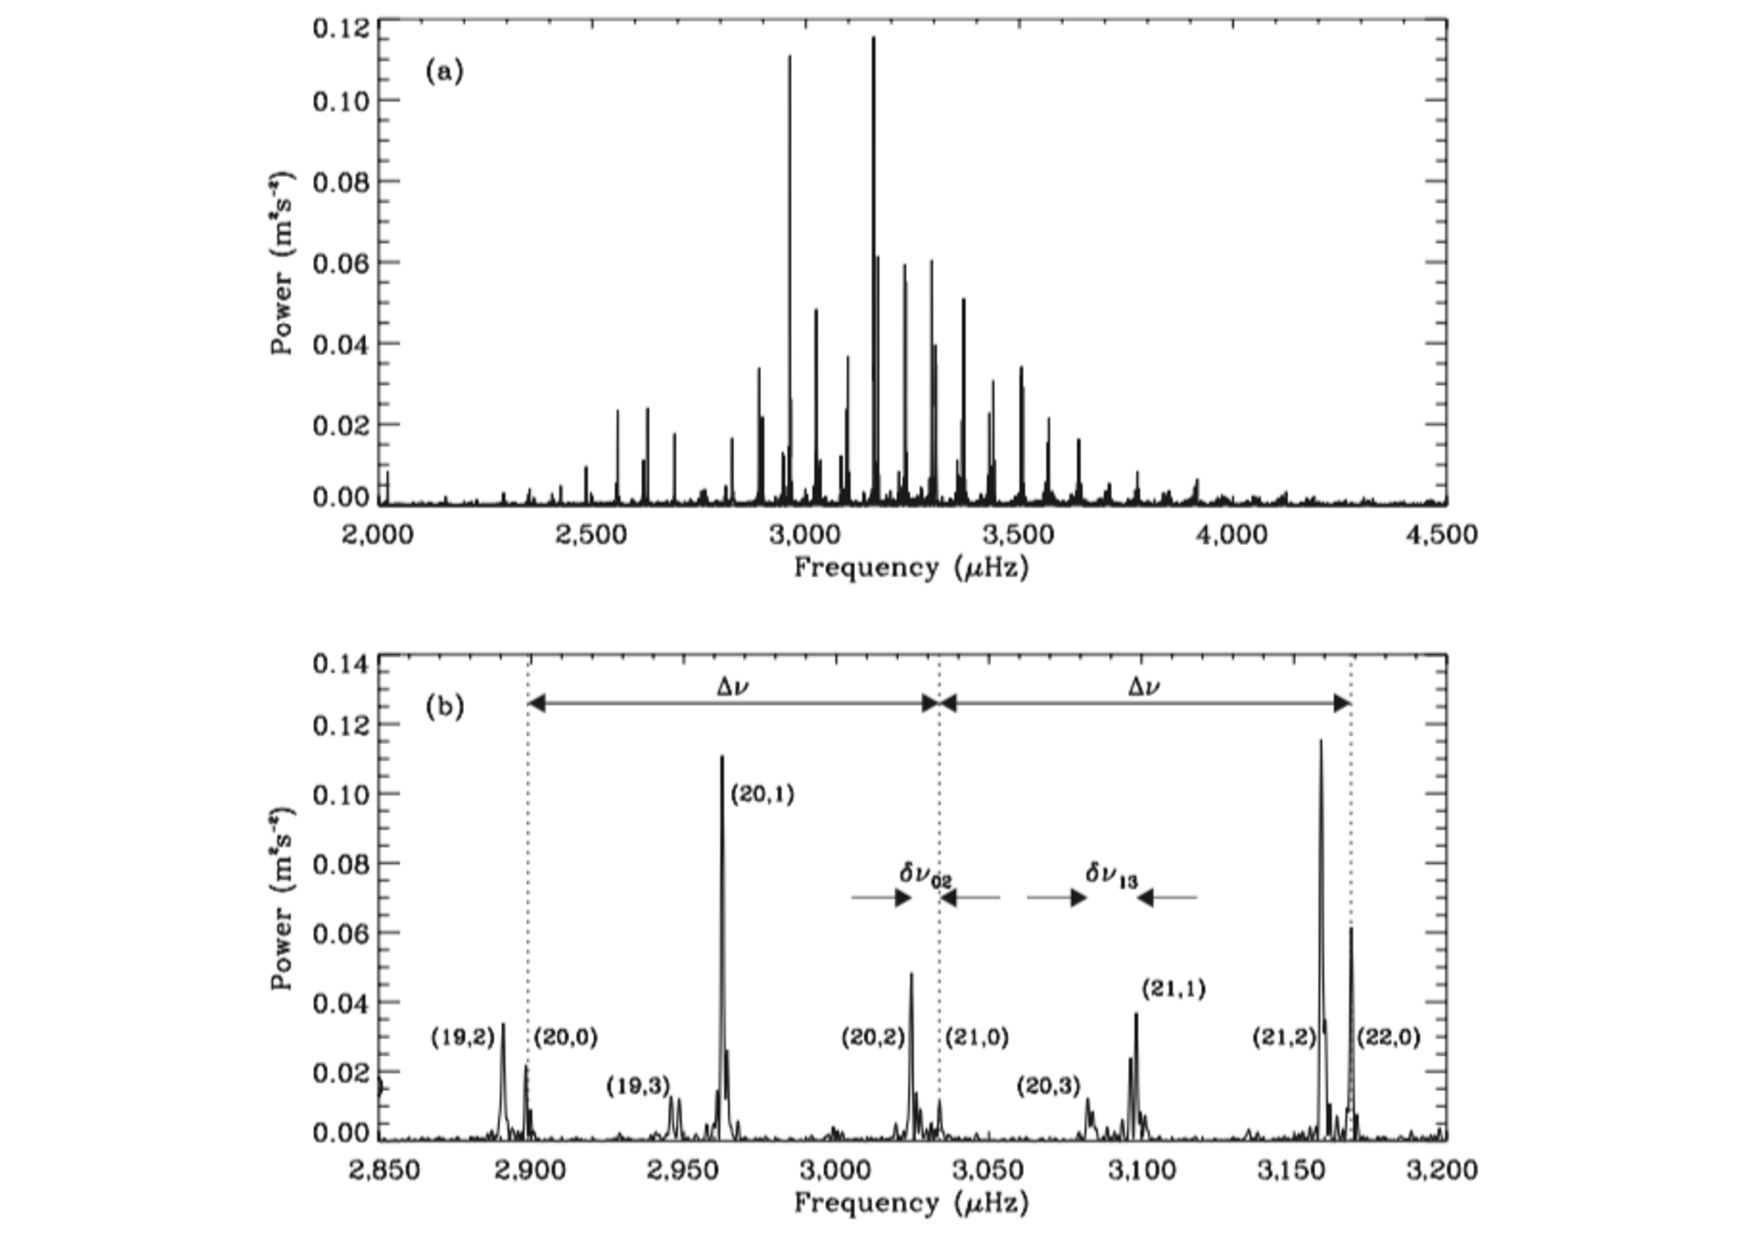
\includegraphics[width=0.95\textwidth]{Figures/1-Introduction/power_spectrum_sun.pdf}
    \caption[Example of solar power spectrum from which asteroseismic analysis can be conducted]{Panel (a) shows the solar power spectrum from ten days of disk-integrated velocity measurements with the BiSON instrument. Panel (b) shows a close-up labelled with (n,l) values for each mode. Dotted lines show the radial modes, and the large and small separations are indicated. Image credit: figure 3.1 from \citet{Palle_Esteban_2014}}
    \label{fig:power_spectrum_example_sun}
\end{figure}

While the parameters defined above come from observations, theoretical studies give physical meaning to these parameters. \citet{Brown_etal_1991} suggested that $\nu_{max}$ might be a a fixed fraction of the acoustic cut-off frequency. The cut-off frequency is defined as a boundary where energy flowing in the system becomes reduced. The acoustic cut-off frequency can be defined by Equation \ref{Eq:acoustic_cut_off_eq} where $c_{s}$ is the speed of sound and $H$ is the density scale height. Density scale height is defined as the vertical distance over which the density falls by a factor of $\frac{1}{e}$. An isothermal approximation of Equation \ref{Eq:acoustic_cut_off_eq} is taken to be $\nu_{ac} \propto \frac{c_{s}}{H}$ which is also proportional to the frequency of maximum power, $\nu_{max}$.

\begin{equation}
    \nu_{ac} = \left(\frac{c_{s}}{4\pi H}\right)^{2}\left(1 - 2\frac{dH}{dr}\right)
    \label{Eq:acoustic_cut_off_eq}
\end{equation}

Assuming the system is adiabatic and that the ideal gas law applies, then the speed of sound squared will be proportional to the temperature. By substituting this and $H \propto \frac{T}{g}$ (which comes from the definition of the scale height), Equation \ref{Eq:v_max_eq} is obtained \citep{Kjeldsen_Bedding_1995}. Note that since oscillations are observed in the photosphere, it is reasonable to assume that the temperature is close to the effective temperature of the star. This equation shows that with a prior on the effective temperature of the star, the surface gravity of a star can be obtained from the measurement of $\nu_{max}$.

\begin{equation}
    \nu_{max} \propto g(T_{eff})^{-\frac{1}{2}}
    \label{Eq:v_max_eq}
\end{equation}

Theoretical calculations using asymptotic theory (e.g. \citealt{Christensen_Dalsgaard_1988}) show that the large frequency separation, $\Delta\nu$, can be defined as the inverse of the sound travel time through the star as shown in Equation \ref{Eq:theoretical_large_freq_separation}.

\begin{equation}
    \Delta\nu \simeq \left(2 \int_{0}^{R} \frac{dr}{c_{s}} \right)
    \label{Eq:theoretical_large_freq_separation}
\end{equation}

If Equation \ref{Eq:theoretical_large_freq_separation} is integrated from the centre to the surface of the star and a substitution for the speed of sound is made (assuming adiabatic conditions) then Equation \ref{Eq:large_freq_step_one} is obtained. $\langle T \rangle$ is the average internal temperature.

\begin{equation}
    \Delta\nu \propto \frac{\sqrt{\langle T \rangle}}{R}
    \label{Eq:large_freq_step_one}
\end{equation}

Finally, a substitution can be made for the average internal temperature where $\langle T \rangle \propto \frac{M}{R}$ as derived from the virial theorem. This leads to Equation \ref{Eq:large_freq_final_eq} where $\langle \rho \rangle$ is the mean stellar density. Thus, the measurement of the large frequency separation leads to the calculation of the mean stellar density.

\begin{equation}
    \Delta\nu \propto \left(\frac{M}{R^{3}} \right)^{\frac{1}{2}} \equiv \sqrt{\langle \rho \rangle}
    \label{Eq:large_freq_final_eq}
\end{equation}

\begin{figure}[t]
    \centering
    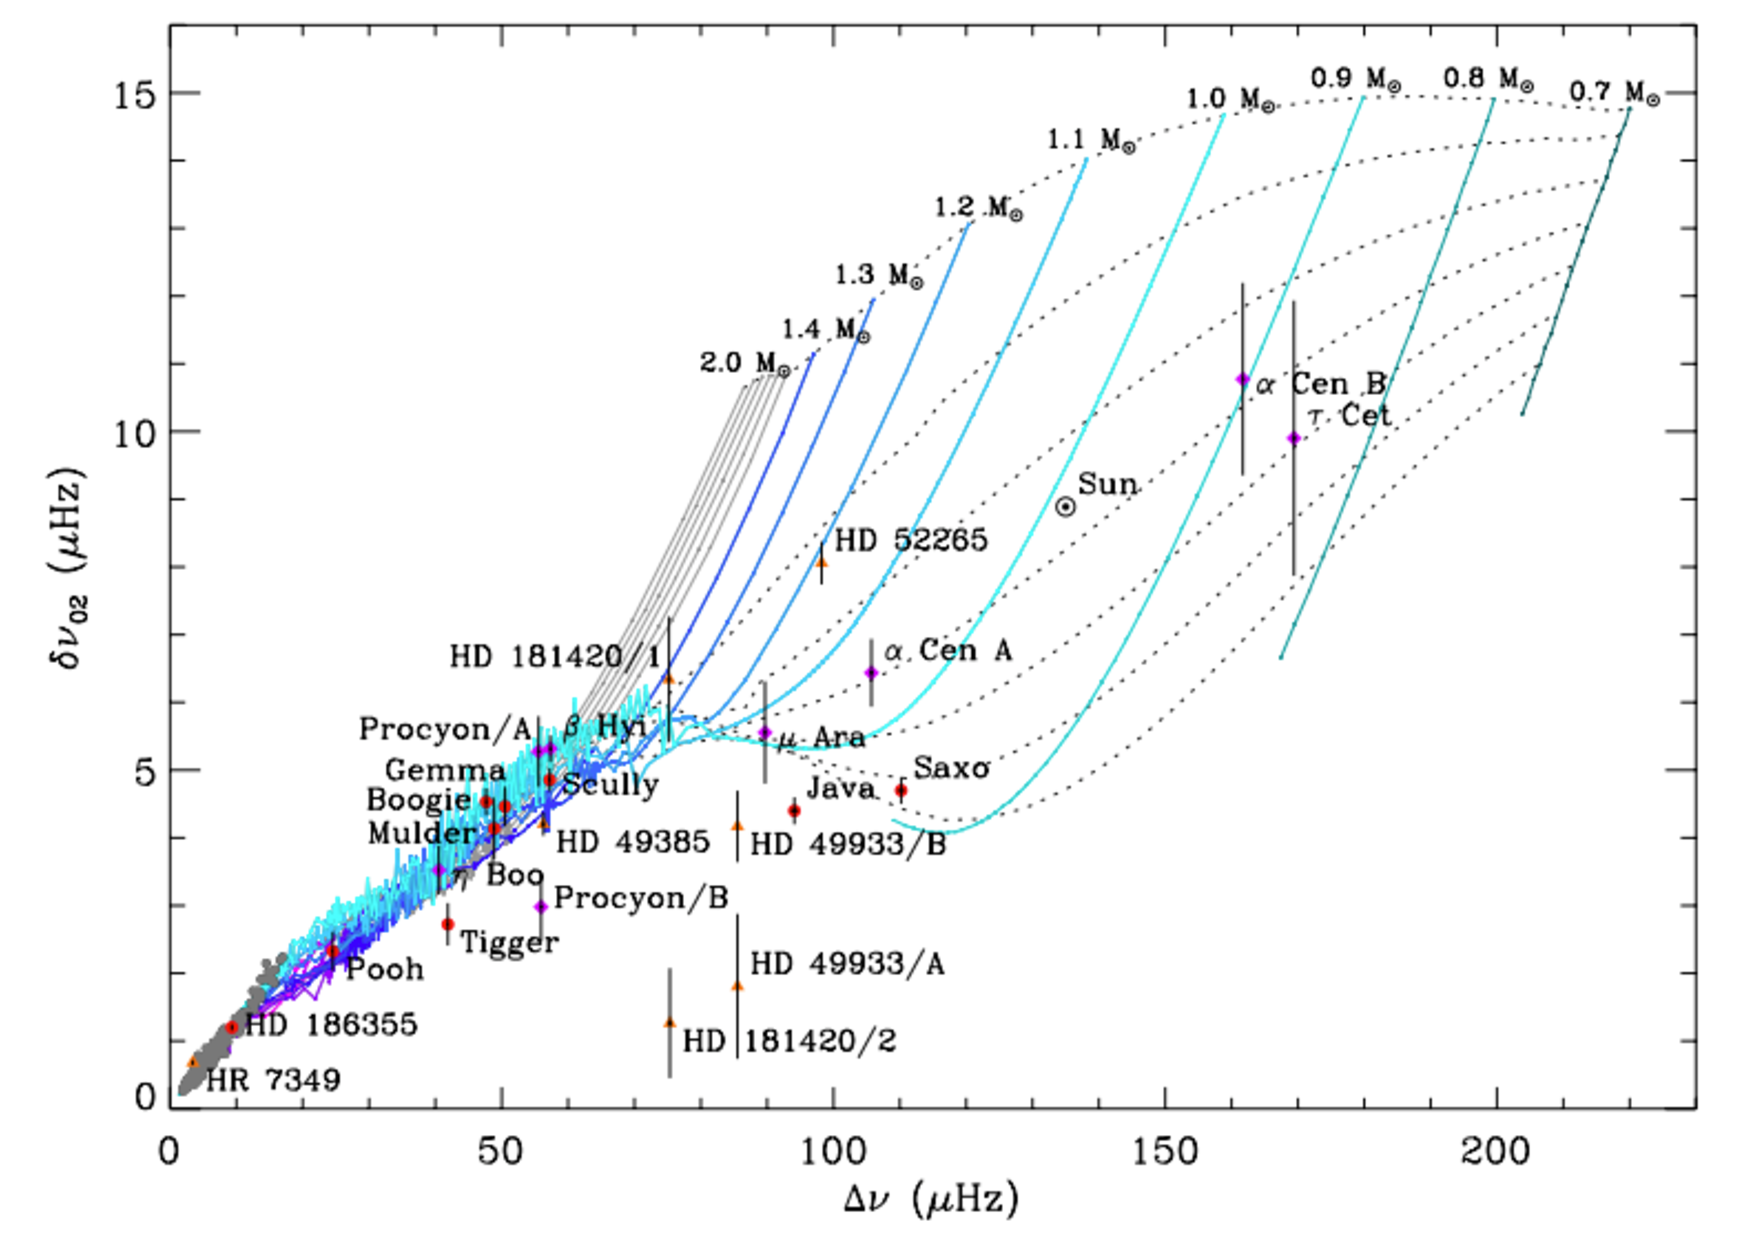
\includegraphics[scale=0.4]{Figures/1-Introduction/C-D_diagram.pdf}
    \caption[C-D diagram used to determine stellar ages]{C-D diagram, with model tracks for near-solar metallicity (Z$_{0}$ = 0.017). Tracks increase in mass by 0.1 M$_{\odot}$ from 0.7 M$_{\odot}$ to 2.0 M$_{\odot}$ as labelled. Dashed black lines are isochrones, increasing by 2 Gyr from 0 Gyr (ZAMS) at the top to 12 Gyr at the bottom. Stars shown were observed using CoRot, Kepler or using ground telescopes. Image credit: \citet{White_etal_2011}}
    \label{fig:CD_diagram_example}
\end{figure}

Lastly, the small frequency separation is related to the age of the star \citep{Ulrich_1986}. \citet{Christensen_Dalsgaard_1984} noted that some frequency differences were dependant on stellar age due to the conversion of hydrogen into helium and the attendant reduction in the speed of sound near the core. Another useful diagnostic tool in asteroseismology is the C-D diagram, first introduced by \citet{Christensen_Dalsgaard_1984}, which plots the small frequency separation as a function of the large frequency separation. One such example is shown in Figure \ref{fig:CD_diagram_example} from \citet{White_etal_2011}, which shows a sample of stars with model tracks for mass and age. In the top right of the plot (corresponding to the main sequence phase), these tracks are sufficiently spread out that masses and ages can be determined for these stars. However, as stars evolve off the main sequence, the model tracks converge for the subgiant and red giant evolutionary phases. One disadvantage to this method is that the model tracks depend on the metallicity: thus to ensure the most accurate parameters, the metallicity of the star must be known.

Asteroseismology has been revolutionised by space--based telescopes such as \textit{CoRoT} and \textit{Kepler}, as they have greatly increased the number of stars with detected solar-like oscillations \citep{Chaplin_etal_2011}. Initially, the global asteroseismic parameters were used alongside complementary photometric and spectroscopic data to estimate stellar parameters \citep{Chaplin_etal_2014}. However, as the baseline for observations from Kepler increased, it became possible to study the individual frequencies, and the precision of the stellar parameters also increased (e.g \citealt{Silva_Aguirre_etal_2015}). Figure \ref{fig:VSA_legacy_uncertainties} shows the distribution of uncertainties for the mean stellar density, radius, mass and age from a number of different pipelines for the Kepler LEGACY sample \citep{Lund_etal_2017}. This sample represents some of the highest signal--to--noise asteroseismic data that is currently available, and we see that typical uncertainties in age are on the order of 10\%, which is a vast improvement on any other age dating method. With current and future space mission such as TESS \citep{Ricker_etal_2015} and PLATO \citep{Rauer_etal_2014}, both of which will further increase the number of stars with detected solar-like oscillations, the future looks bright for asteroseismology.

\begin{figure}
    \centering
    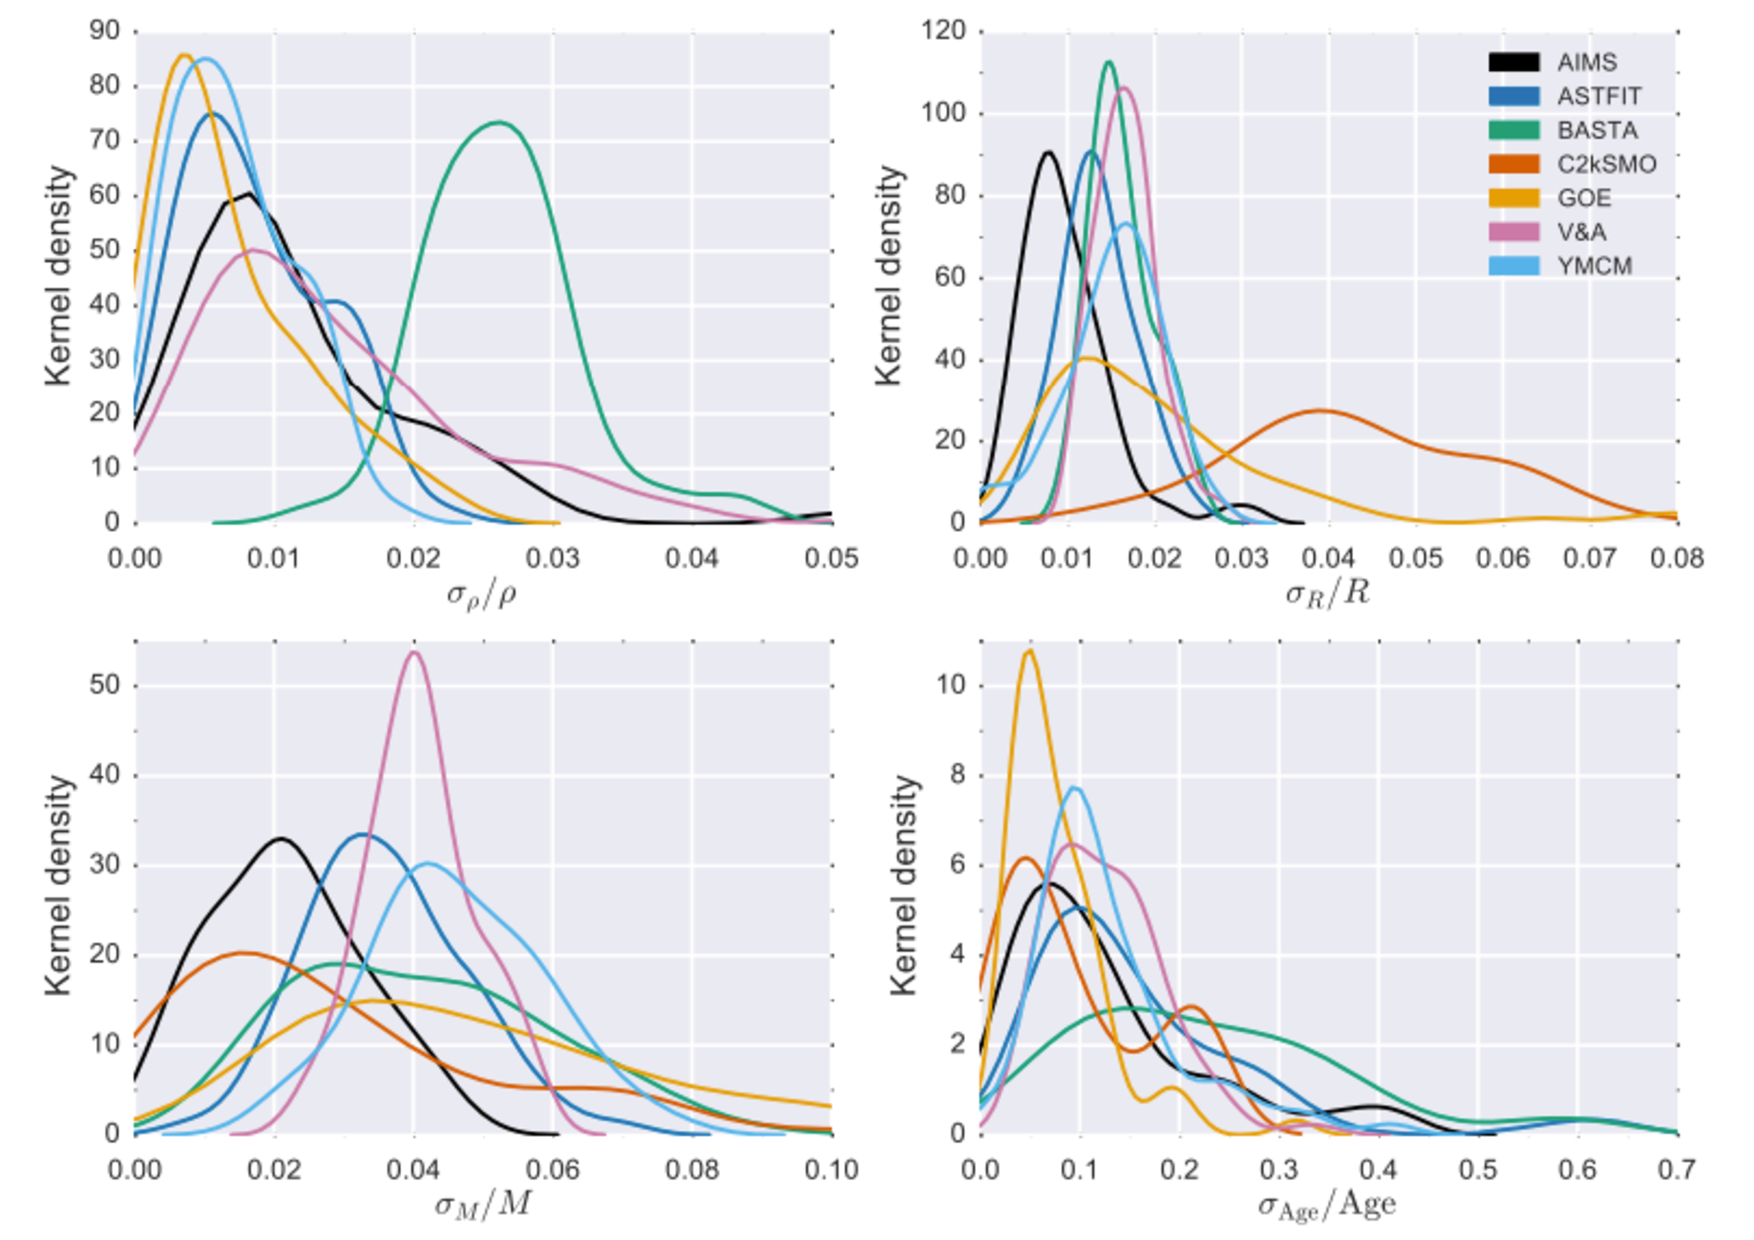
\includegraphics[scale=0.4]{Figures/1-Introduction/silva_aguirre_2017_legacy.pdf}
    \caption[Distributions of uncertainties in asteroseismically determined parameters]{Distributions of uncertainties of various stellar parameters for the whole Kepler LEGACY sample from a number of different pipelines. These stellar parameters are density, radius, mass and age. Image credit: \citet{Silva_Aguirre_etal_2017}}
    \label{fig:VSA_legacy_uncertainties}
\end{figure}

Yet like any other method, asteroseismology also has its disadvantages. For example, there is evidence that the magnetic activity of the star affects the detection of solar-like oscillations \citep{Chaplin_etal_2011_stellar_activity} suggesting that magnetic activity inhibits the amplitude of such oscillations. In addition to this, the intrinsic amplitude of the oscillations means that they are easier to detect in early-type and more evolved stars \citep{Houdek_etal_1999}. Therefore such asteroseismic samples may be biased to low--activity and more evolved stars, and this must be taken into consideration for such samples. Also, in order to gain the highest signal--to--noise asteroseismic data (and therefore the most precise stellar parameters), observations must be taken over a long period of time. This will only be possible for a fraction of the stellar population. How can we determine ages for stars that have not been studied using asteroseismology?

\subsection{Empirical age relations}
An alternative way of determining ages for stars is to use empirical age relationships. This method takes a stellar parameter and shows how it evolves in time, therefore making it possible to infer an age for a star from a single parameter. In these relationships, a plausible physical mechanism works to cause the change in the stellar parameter over time, but the exact physics underlying it is not fully understood. Furthermore, these relationships must first be calibrated by studying these stellar parameters for stars with known ages. Ages are typically calculated using one of the model-dependent methods described previously, making these empirical relationships secondary to the model-dependent methods of determining ages. However, they can provide an estimate of the star's age where no other method can be used.

As discussed previously, in solar-like and low-mass stars there exists a dynamo mechanism that links the rotation and magnetic field of the star. Through magnetic braking over the main sequence lifetime of a star, we expect the star to lose angular momentum. This causes an increase in the observed rotation period of the star and consequently a decrease in the overall magnetic activity of the star. For this reason, rotation and magnetic activity are commonly used in these empirical relationships.

It is these empirical age relationships (particularly the age--activity relationship) that are the focus of the research presented in this thesis. While they may be a secondary method of determining ages in comparison to the model-dependent ages, they are important in the understanding of the physical processes that underpin them. From constraining the age--activity relationship, we gain new information in how the stellar wind and dynamo change over the main sequence lifetime of a star. In Chapter \ref{Chapter2}, an overview of previous work concerning the age--activity--rotation relationship will be discussed.

\section{Structure of Thesis}
In this thesis I present a study primarily on the age--activity relationship that aims to study the older regime of the relationship (i.e. $> 1$~Gyr). This is achieved by considering ages determined from asteroseismology combined with relevant observations for determining the X-ray luminosity and chromospheric emission. Literature rotation periods will also be used to try and link the age--activity samples to the stellar rotational evolution. In this chapter I have given an overview of some of the key aspects needed in order to fully appreciate the underlying mechanisms at work in the age--activity--rotation relationship.

In Chapter 2, I will give an historical overview of the previous work that has been conducted concerning the age--activity--rotation relationship, including the current limitations and regimes where the relationship is not fully understood. Chapter 3 is a study on the age--activity relationship using X-ray observations and asteroseismic ages for stars older than a gigayear. Chapter 4 details an investigation into the chromospheric emission as a function of age using optical spectra data and asteroseismic ages. Chapter 5 attempts to piece together the age--activity relationships determined in previous chapters with rotational data. Finally, in Chapter 6 I will give a summary of the main conclusions of my work and highlight the future prospects of the field.
% Chapter Template

\chapter{History of age-activity-rotation relationships} % Main chapter title

\label{Chapter2} % Change X to a consecutive number; for referencing this chapter elsewhere, use \ref{ChapterX}

%----------------------------------------------------------------------------------------
%	SECTION 1
%----------------------------------------------------------------------------------------

\epigraph{\itshape The past can hurt. But the way I see it, you can either run from it or learn from it.}{---Rafiki, \textit{The Lion King}}

\section{Introduction}

The history of age-activity-rotation studies dates back to the 1960's, when the theoretical framework for these relationships (i.e. magnetic braking) was first theorised by \citet{Schatzman_1962}. \citet{Wilson_1963} first suggested that emission in \caII lines (and chromospheric activity in general) declined with stellar age. This was based off observations that the average intensity of \caII emission was much higher for main-sequence stars in several clusters (including Hyades and Praesepe) than for local field stars. \citet{Kraft_1967} suggested the same concerning rotation based off a sample of rotational velocities ($vsin(i)$) for a large sample of field stars with the average rotational velocity being higher for stars with \caII emission than those without. Since there was evidence that the \caII emission declined with age then so must the rotational velocity.

Probably the most cited paper concerning activity, rotation and their evolution in time is the seminal paper by \citet{Skumanich_1972}. This paper was the first to plot activity and rotation as a function of age using data from the Pleiades, Ursa Major, Hyades and the Sun as shown in Figure \ref{fig:Skumanich_plot}. Skumanich found that the calcium emission and rotational velocities followed a power law: $Ca^{+} \propto \tau^{-\frac{1}{2}}$ where $\tau$ is the stellar age. This power law is commonly known as the Skumanich Law and studies still compare results to it. The rest of this section will highlight some of the most relevant papers that document the progress of the age-activity-rotation relation, what has been achieved and what can still be improved upon.

\begin{figure}
    \centering
    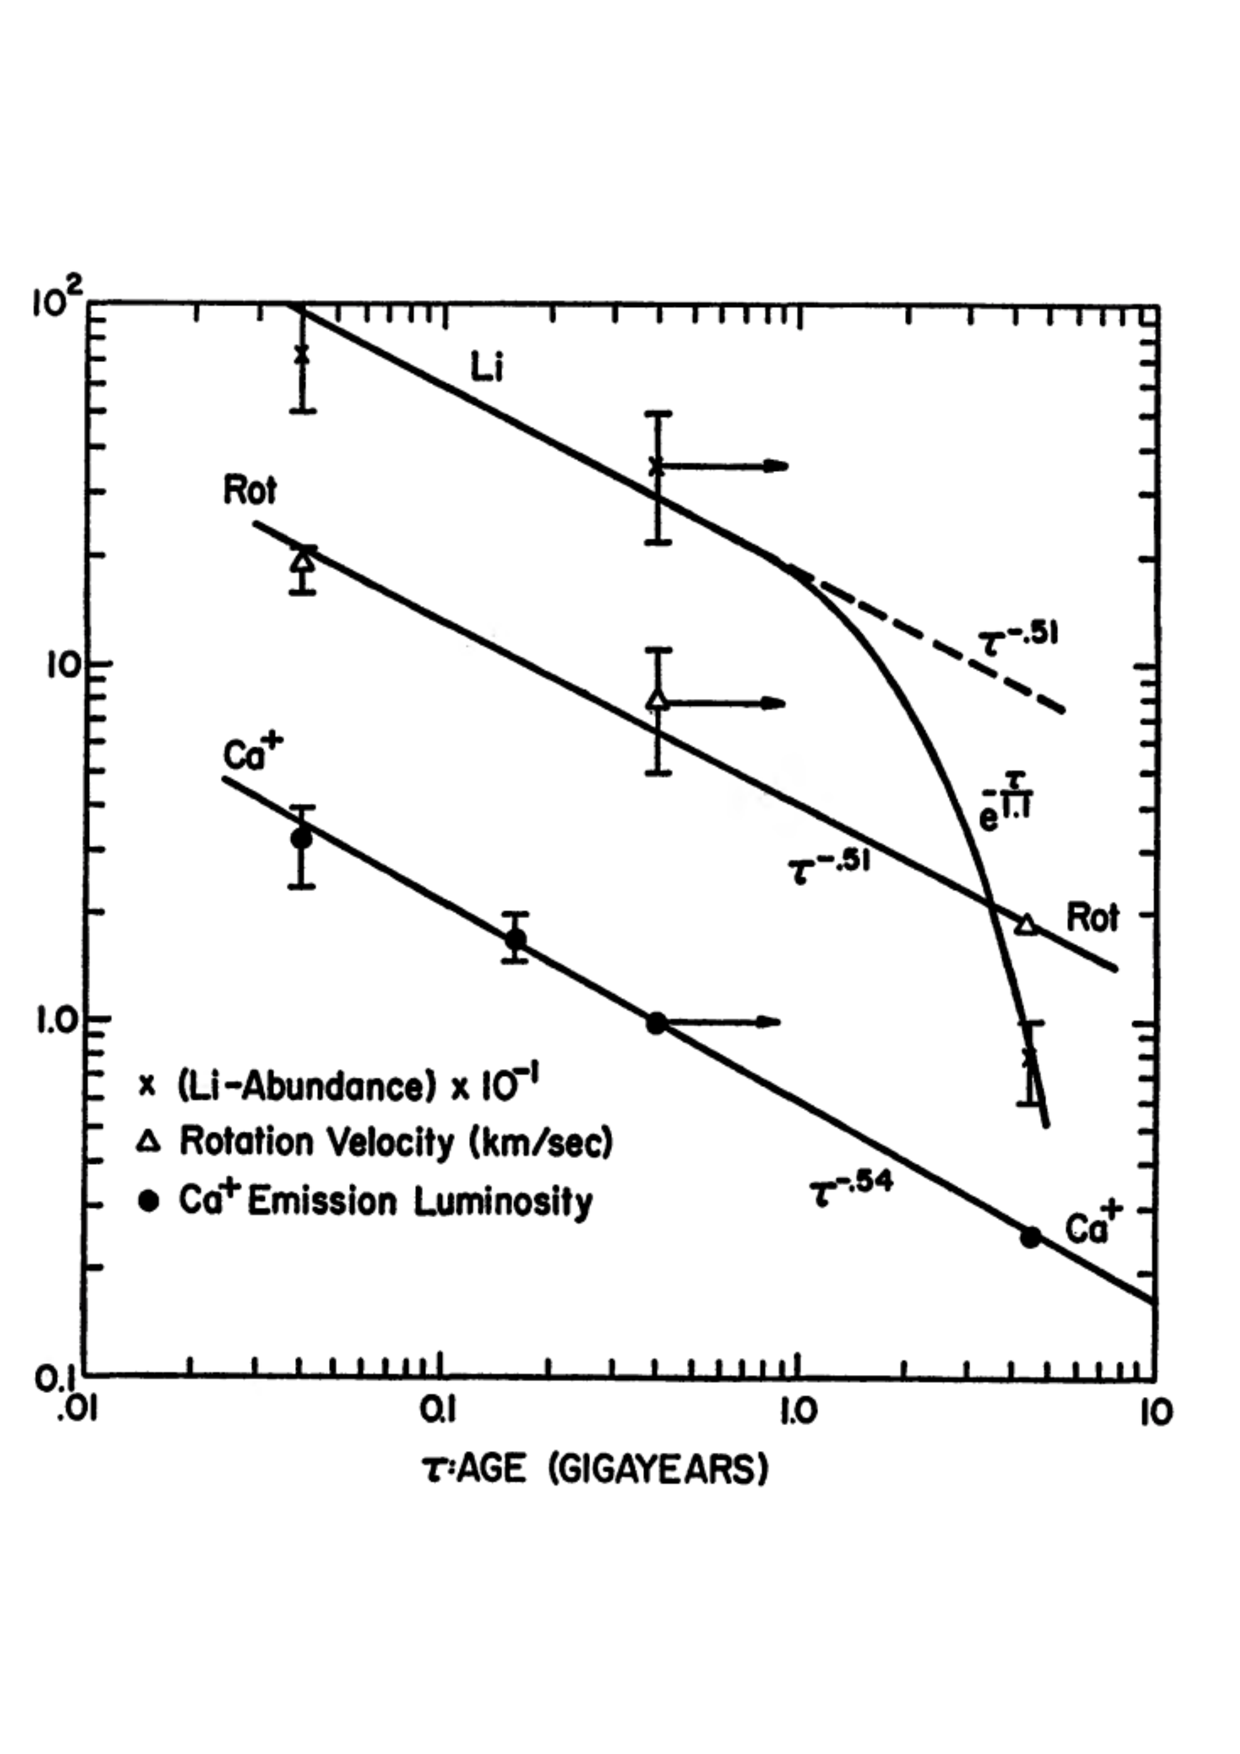
\includegraphics[scale=0.45]{Figures/2-Historical_overview/skumanich_1972.pdf}
    \caption[First plot of age-activity-rotation relationship]{Calcium emission, lithium abundance and rotational velocity as a function of age for two clusters and the Sun. The solid lines represent the Skumanich law - $\propto \tau^{-\frac{1}{2}}$ Image credit: \citet{Skumanich_1972}}
    \label{fig:Skumanich_plot}
\end{figure}

\section{Age-rotation studies (Gyrochronology)}
The term generally used to denote the age-rotation relationship is "gyrochronology" which originates from the seminal paper by \citet{Barnes_2003}. The general relationship between the rotational velocity and age can be written as shown in Equation \ref{Eq:general_rotation_age}, this will become important for Section \ref{Chp2_section_activity_age}.

\begin{equation}
    v_{rot} \propto t^{\alpha}
    \label{Eq:general_rotation_age}
\end{equation}

\citet{Barnes_2003} gathered rotation periods for a number of open clusters alongside old Mount Wilson stars allowing for a wide variety of stars to be studied together. The rotation periods for each cluster/group are plotted as a function of (B-V) colour as shown in Figure \ref{fig:barnes_2003_plot}. From these plots, \citet{Barnes_2003} was able to identify several sequences with the most important two for this discussion being the I and C sequence, later termed the Interface and Convective sequences (pertaining to the type of dynamo present, see \citet{Barnes_2003} for a full discussion).

\begin{figure}
    \centering
    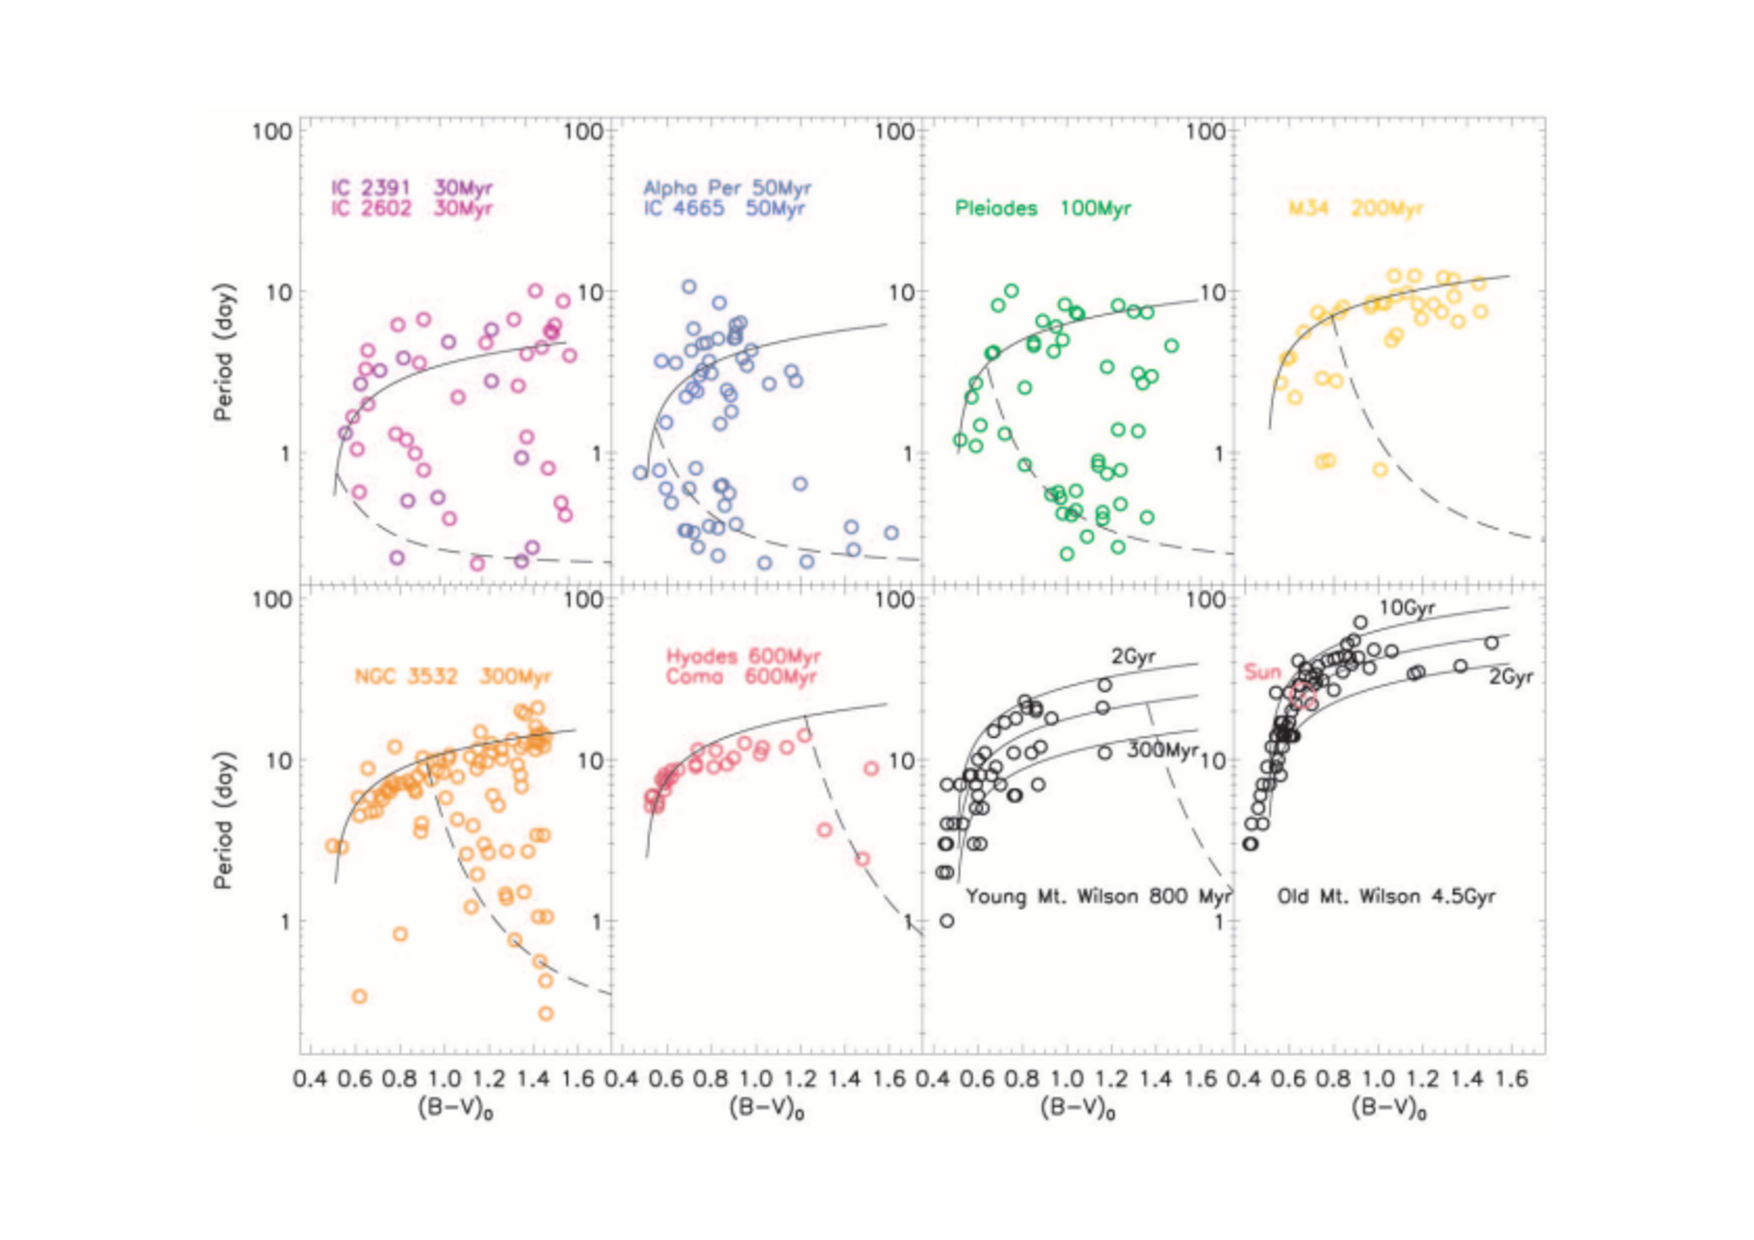
\includegraphics[scale=0.5]{Figures/2-Historical_overview/barnes_2003.pdf}
    \caption[Rotation period as function of colour for a number of clusters]{Plot of rotation period as a function of (B-V) colour for a number of clusters and a sample of Mount Wilson stars which are divided up into young and old ages. Dashed lines indicate the position of the I and C sequences (see text for details).}
    \label{fig:barnes_2003_plot}
\end{figure}

The I sequence is a diagonal band of increasing period with increasing (B-V) colour which is only faintly visible in the youngest cluster but becomes more pronounced as one proceeds to older ages. It also accounts for an increasingly large fraction of stars as in the Hyades cluster all but three stars lie on this sequence and the sequence is non-existent in the Mount Wilson sample. The positive slope of this sequence also increases with stellar age indicating that lower mass stars spin down faster and higher mass stars spin down slower or hardly at all.

In the youngest clusters, a sequence of ultra-fast rotators (UFR's) are also observed and known as the C sequence. This sequence bifurcates away form the I sequence towards shorter rotation periods. Initially this sequence is well populated and becomes increasingly sparse with age, it also seems to be lifted with time towards longer rotation periods. \citet{Barnes_2003} noted that the C sequence never crosses the I sequence but the point at which it starts bifurcating from the I sequence moves to redder values of (B-V) colour with age. The decreasing population of the C sequence also suggests that stars move from the C to I sequence over time. The region between the two sequences is known as the gap and is also often populated. However, this is more sparsely populated than the other two sequences. It's population density also decreases with age. This also fits in with the theory that stars move from the C to I sequence.

\citet{Barnes_2003} also determined a formula for using rotation as an age indicator once stars have converged onto the I sequence. This formula shown in Equation \ref{Eq:B03_eq_1} shows that the rotation period is both dependent on the age of the star and the colour; note that this relationship is consistent with the Skumanich law. Equation \ref{Eq:B03_eq_2} shows the dependence on the colour parameter. If these equations are plotted for a given age and a range of colours, this results in a rotational isochrone, opening up the possibility of dating clusters by looking at fundamental parameters.

\begin{equation}
    P_{rot} = \sqrt{t}f(B-V)
    \label{Eq:B03_eq_1}
\end{equation}

\begin{equation}
    f(B-V) = \sqrt{(B-V) -0.5} - 0.15(B-V-0.5)
    \label{Eq:B03_eq_2}
\end{equation}

Further work was conducted by \citet{Barnes_2007} to improve the gyrochronology relationship in order to determine ages for field stars. They derived a formula using open clusters ranging from 30 - 600 Myr in age. The clusters enabled the mass dependency to be determined to a higher accuracy as they contain a large range of masses for a given age; the mass dependency found by \citet{Barnes_2007} is given by Equation \ref{Eq:B07_mass_eq}.

\begin{equation}
    f(B-V) = 0.7725(B-V-0.4)^{0.601}
    \label{Eq:B07_mass_eq}
\end{equation}

The age dependence was based off the solar value as it has the best known rotation period. The solar values for rotation period, age and (B-V) colour were used to determine the exponent of the age dependency shown in Equation \ref{Eq:B07_age_eq}. Therefore to determine the rotation period for a star of a given age and colour Equation \ref{Eq:B07_combine_eq} could be used. \citet{Barnes_2007} derived errors for ages and found that these were typically $\sim 15$\% not including systematics.

\begin{equation}
   g(t) = t^{0.5189}
    \label{Eq:B07_age_eq}
\end{equation}

\begin{equation}
    P(B-V, t) = f(B-V)g(t)
    \label{Eq:B07_combine_eq}
\end{equation}

In order to test these updated relations derived in \citet{Barnes_2007}, a comparison was made to chromospheric ages which showed good agreement. Ages were also calculated for individual members of binary systems and they found that the binary members showed the same age giving confidence to the relations determined in the paper.

However, more clusters were needed to confirm the existing gyrochronology relationships. One notable breakthrough in this regard was the study of the 2.5 Gyr old cluster NGC 6819 by \citet{Meibom_etal_2015}. A sample of 30 cool stars ranging from 0.85 to 1.4 solar masses with rotation periods determined from Lomb-Scargle periodograms of long-cadence Kepler data were analysed. The data for this cluster was plotted alongside previous cluster data (as shown in Figure \ref{fig:Meibom_etal_2015_plot}) and found to agree with previous gyrochronology relationships. This study bridged a gap in observational data between the Hyades cluster and solar values and provided confirmation in existing gyrochronology relationships.

\begin{figure}
    \centering
    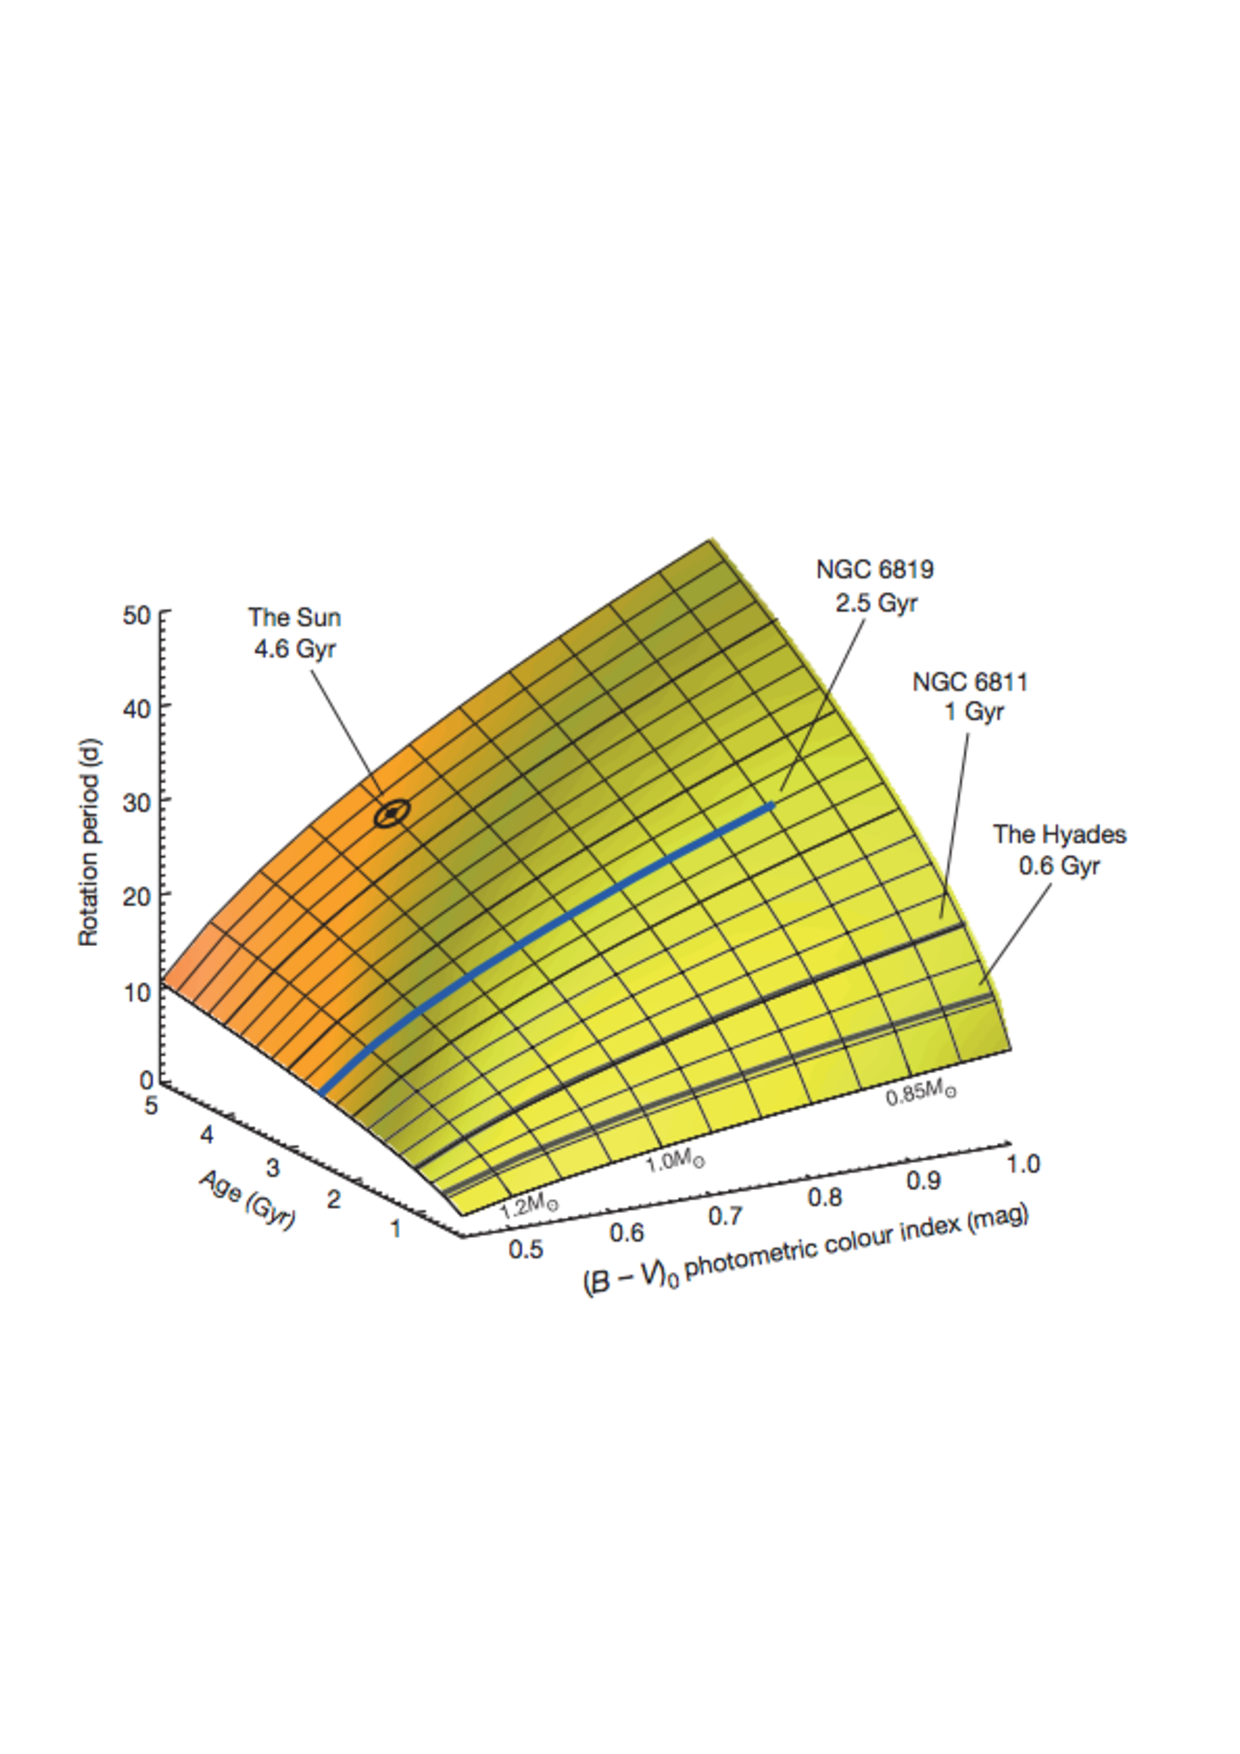
\includegraphics[scale=0.55]{Figures/2-Historical_overview/meibom_etal_2015.pdf}
    \caption[Comparison of data from 2.5 Gyr old cluster to previous gyrochronology relationship]{Observations of rotation periods from NGC 6819 alongside younger clusters and solar values. Yellow surface represents the typical gyrochronology relationship which shows good agreement with the cluster data. Image credit: \citet{Meibom_etal_2015}}
    \label{fig:Meibom_etal_2015_plot}
\end{figure}

At this stage in the literature, the cluster observations seemed to be confirming that if the mass (or colour) of the star is taken into consideration then the rotation period could be used to date the star. But with the launch of Kepler, the field of asteroseismology had been rapidly expanded to detect even more solar-like oscillators for which ages could be determined for \citep{Chaplin_etal_2011}. The first attempt at extending gyrochronology to older ages by considering asteroseismic ages was by \citet{Angus_etal_2015}.

This study considered 310 Kepler stars with asteroseismic ages, 50 stars from the Hyades and Coma Berenices clusters and 6 field stars with precise ages (including the Sun). \citet{Angus_etal_2015} calibrated a relation in the form shown in Equation \ref{Eq:Angus_etal_2015_eq} where A is the age in Myr and the free parameters fitted are a, b, c and n. The best-fitting values for these parameters were: a=0.40, b-0.31, c=0.45 and n=0.55.

\begin{equation}
    P = A^{n}a(B - V - c)^{b}
    \label{Eq:Angus_etal_2015_eq}
\end{equation}

\citet{Angus_etal_2015} also investigated the posterior probability distribution function of the gyrochronology parameters, including an analysis of different subsets of the data. This analysis found tension between the asteroseismic ages and the gyrochronology relation as no single relation could adequately describe all subsets of the data. this provided concerns over the use of gyrochronology as an age dating method. It is worth noting that the asteroseismic ages used in \citet{Angus_etal_2015} were calculated from global modelling of the asteroseismic parameters which are known to be more uncertain than when individual frequencies are modelled.

\begin{figure}
    \centering
    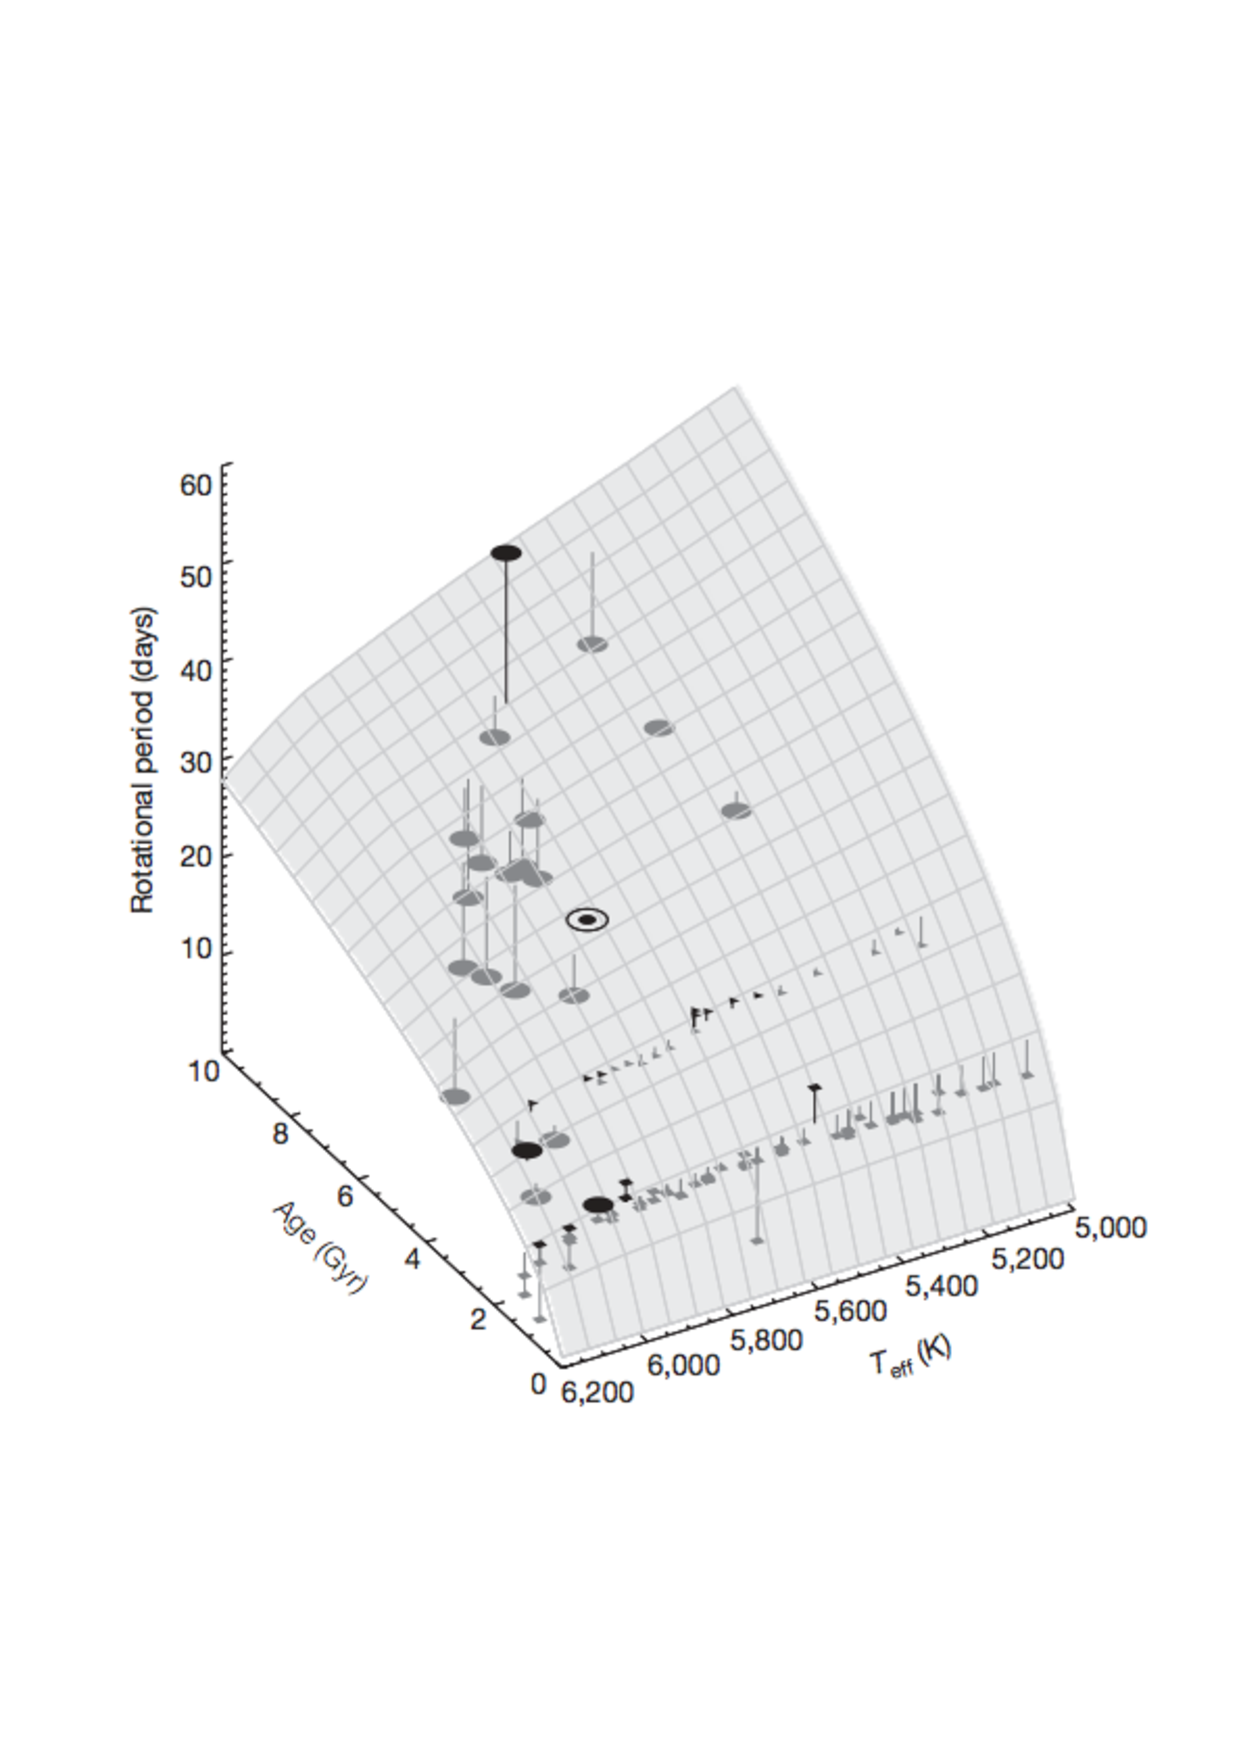
\includegraphics[scale=0.45]{Figures/2-Historical_overview/van_saders_3d_plot.pdf}
    \caption[Comparison of older sample of stars to previous gyrochronology relaitonship and cluster data]{Plot of rotation period, effective temperature and age for \citet{van_Saders_etal_2016} sample alongside cluster data. An empirical relationship is also shown. Image credit: \citet{van_Saders_etal_2016}}
    \label{fig:van_saders_plot_1}
\end{figure}

\begin{figure}[h]
    \centering
    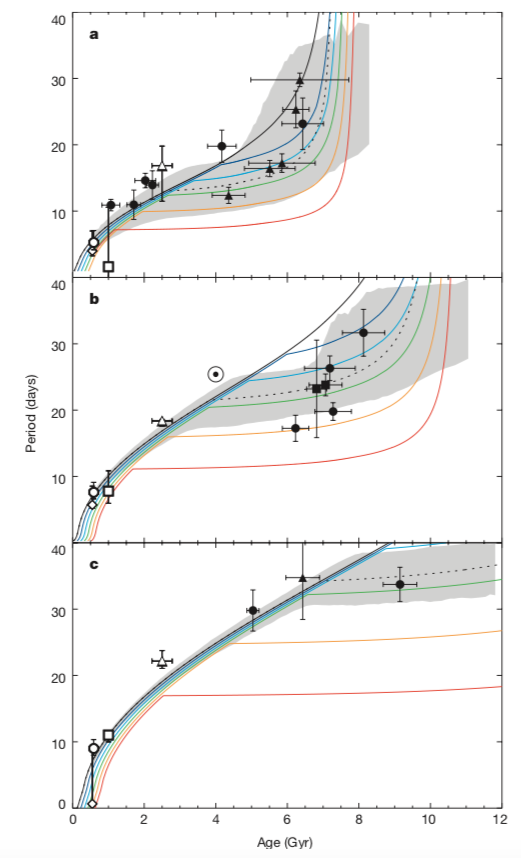
\includegraphics[scale=0.35]{Figures/2-Historical_overview/van_saders_R0_plot.png}
    \caption[Rotation period as a function of age with various stellar models that include a critical Rossby number]{Plot of rotation period as a function of age  for \citet{van_Saders_etal_2016} sample alongside cluster data divided into three effective temperature ranges from hottest in the top (a) panel and coolest in bottom (c) panel. Curves represent various stellar models with different critical Rossby numbers ranging from 0 (black line) to 3.0 (red). Dashed line shows best fit for critical Rossby number of $R_{0} = 2.16$. Image credit: \citet{van_Saders_etal_2016}}
    \label{fig:van_saders_plot_2}
\end{figure}

The tension between asteroseismic ages and gyrochronology increased when \citet{van_Saders_etal_2016} presented a sample of field stars with precise asteroseismic ages from individual frequency modelling. Their sample consisted of 21 Kepler stars with high precision ages, rotation periods from photometric variability and measured metallicities. Figure \ref{fig:van_saders_plot_1} shows the empirical gyrochronology relationship and the observed rotation periods for the \citet{van_Saders_etal_2016} sample of stars, they found that the majority of their sample of stars lay below the empirical surface. They found that stars more evolved than the Sun showed rapid rotation which persisted across a range of effective temperatures and they interpreted this as weakened magnetic braking.

\citet{van_Saders_etal_2016} postulated that above a critical value the effective loss of angular momentum stopped; this critical value was considered in term of Rossby Number. The Rossby number ($R_{0}$) is defined as the rotation period divided by the convective turnover time ($\tau_{c}$) and is commonly used in the activity-rotation relationship (see Section \ref{Chp2_activity-rotation_lit_review}). The convective turnover time is defined as the typical timescale taken for a convective cell to rise and is dependent on the mass of the star as this is the main parameter that determines the depth of the convection zone. To test this hypothesis, \citet{van_Saders_etal_2016} modified stellar models to conserve angular momentum above a certain critical $R_{0}$. Figure \ref{fig:van_saders_plot_2} shows cluster data and the sample of older stars with various stellar angular momentum models with the inclusion of the critical Rossby number. \citet{van_Saders_etal_2016} find the best critical Rossby number is 2.16 which is able to explain both the the young cluster data and old sample of stars. This results cast doubt on the use of rotation period as an age indicator as it may only work for part of the stellar population. Note that the age at which the gyrochronology relation is no longer valid, according to this result, is different for varying stellar masses. The data in panel (b) of Figure \ref{fig:van_saders_plot_2} would suggest that the Sun is on the cusp of the transition to weakened magnetic braking.

%Insert dos Santos, L +2016 paper
Further evidence for a modified braking law for solar-

\textcolor{red}{FINISH THIS PARAGRAPH}



Despite the tension between gyrochronology and asteroseismic ages, research continued to extend the relationship using clusters. \citet{Barnes_etal_2016} reported rotation periods for 20 cool (FGK) stars in the 4 Gyr old M67 cluster with data from the K2 mission. Rotation periods were determined from the 75 day baseline data with four different methods. The authors do note that the length of the baseline is long enough for starspot evolution but not long enough for multiple phases of periodic variations due to starspots.

\citet{Barnes_etal_2016} plot the rotation period as a function of (B-V) colour and saw a similar shape to that seen in younger clusters (see Figure \ref{fig:barnes_2003_plot} for shape). Therefore, they conclude that since M67 shows a cross section of the gyrochronology surface at an age of 4 Gyr, gyrochronology relations are valid to at least solar age. The study also calculated gyrochronology ages for the individual cluster members of M67 and found a standard deviation from the true cluster age of 0.7 Gyr which is equivalent to approximately 17\%. The authors suggest that similar errors could be achieved for ages of K2 planet hosts.

However, there are possible limitations to determining rotation periods for older clusters using data from K2. \citet{Esselstein_etal_2018} presented a sample of comprehensive injection tests into M67 light curves from the K2 campaign (i.e. the same data \citealt{Barnes_etal_2016} used) and they attempt to recover the injected signals with a Lomb-Scargle periodogram analysis. While they find that the reliability of the detected rotation periods are high, they also find that the sensitivity drops rapidly with increasing rotation period and decreasing amplitude. In the case of a solar rotator, they find that there is only a 15\% recovery rate. This study highlighted the need for caution when determining rotation periods for any cluster observed by K2 or similar missions such as TESS.

In \citet{Barnes_etal_2016_aspect_gyro}, the authors discuss the implications of the claimed weakened magnetic braking by \citet{van_Saders_etal_2016}. They claim that the transition at 2.5 Gyr (for stars with effective temperatures: $5900 < T_{eff} < 6200 K$) is ruled out due to the observations of M67 \citep{Barnes_etal_2016} that obey previous gyrochronology laws. However, one could also argue that \citet{Barnes_etal_2016} only had two stars within a similar colour range; this result based on two data points is not statistically significant, perhaps more data is needed to confirm this argument.

\citet{Barnes_etal_2016_aspect_gyro} also argue that other factors could be at fault for the sudden change in rotation periods at older ages and that it may not be a change in the angular momentum evolution. They considered the sample used in \citet{van_Saders_etal_2016} and removed several stars from the sample including stars with $\log(g) < 4.2$ which are post-turnoff stars. They also removed four metal poor stars and 16 Cyg A and B whose seismic rotation periods are incorrect (however, they do not state the reason why they are incorrect). For the remaining eight stars, they found that the gyrochronology ages (as calculated from \citealt{Barnes_2010}) and asteroseismic ages show good agreement.

More recently, \citet{van_Saders_etal_2018} have considered the challenges of interpreting large data sets such as the Kepler data set. In this study, they combine theoretical models of stellar rotation, stellar population model for the galaxy and prescriptions for observational biases to predict the rotational distribution in the Kepler field. The conclusions from the study were firstly that the standard breaking models fail to reproduce the observed distribution at long rotation periods and secondly, that the interpretation of the rotational distribution is complicated by mixtures of unevolved and evolved stars alongside observational uncertainties. \citet{van_Saders_etal_2018} define a threshold Rossby number of 2.08, this is the Rossby edge above which long period high Rossby number stars are either absent or undetected. Note that this value is comparable to the critical Rossby value of 2.16 found in \citet{van_Saders_etal_2016}. The authors conclude that either modified braking is in operation of the full Kepler population or stars undergo a transition in their starspot configuration at a similar Rossby number.

\section{Activity-rotation studies}
\label{Chp2_activity-rotation_lit_review}

From stellar dynamo theory (see Section \ref{Section:intro_dynamo_and_braking_section}), it is known that the stellar magnetic field (and thus magnetic activity) is linked to the rotation of the star through the dynamo effect. Hence it is expected that the magnetic activity and rotation period should be correlated in some way, this has led to several investigations of the activity-rotation relationship which shall be discussed in this section. The general expression for the activity-rotation relationship (in terms of X-ray luminosity) is shown in Equation \ref{Eq:general_activity_rotation}.

\begin{equation}
    L_{x} \propto P_{rot}^{\beta}
    \label{Eq:general_activity_rotation}
\end{equation}

The earliest study of this kind was conducted by \citet{Pallavicini_etal_1981} who analysed the relationship between X-ray luminosity and rotational velocities for stars of varying spectral types and luminosity classes using data from Einstein. In order to study the rotational aspect of the relationship, the study used rotational velocities as calculated from line broadening of spectral lines - $v\sin(i)$ where $v$ is the equatorial velocity and $i$ is the inclination angle. For late type stars (G-M), \citet{Pallavicini_etal_1981} plotted X-ray luminosity as a function of rotational velocities (as shown in Figure \ref{fig:pallavicini_etal_1981_plot}) and found the best fitting relationship as shown in Equation \ref{Eq:pallavicini_81}. The authors do emphasise that the data is still fairly scarce and that new high-sensitive data is needed but as we shall see from more recent studies, this relationship found by \citet{Pallavicini_etal_1981} holds up fairly well.

\begin{figure}
    \centering
    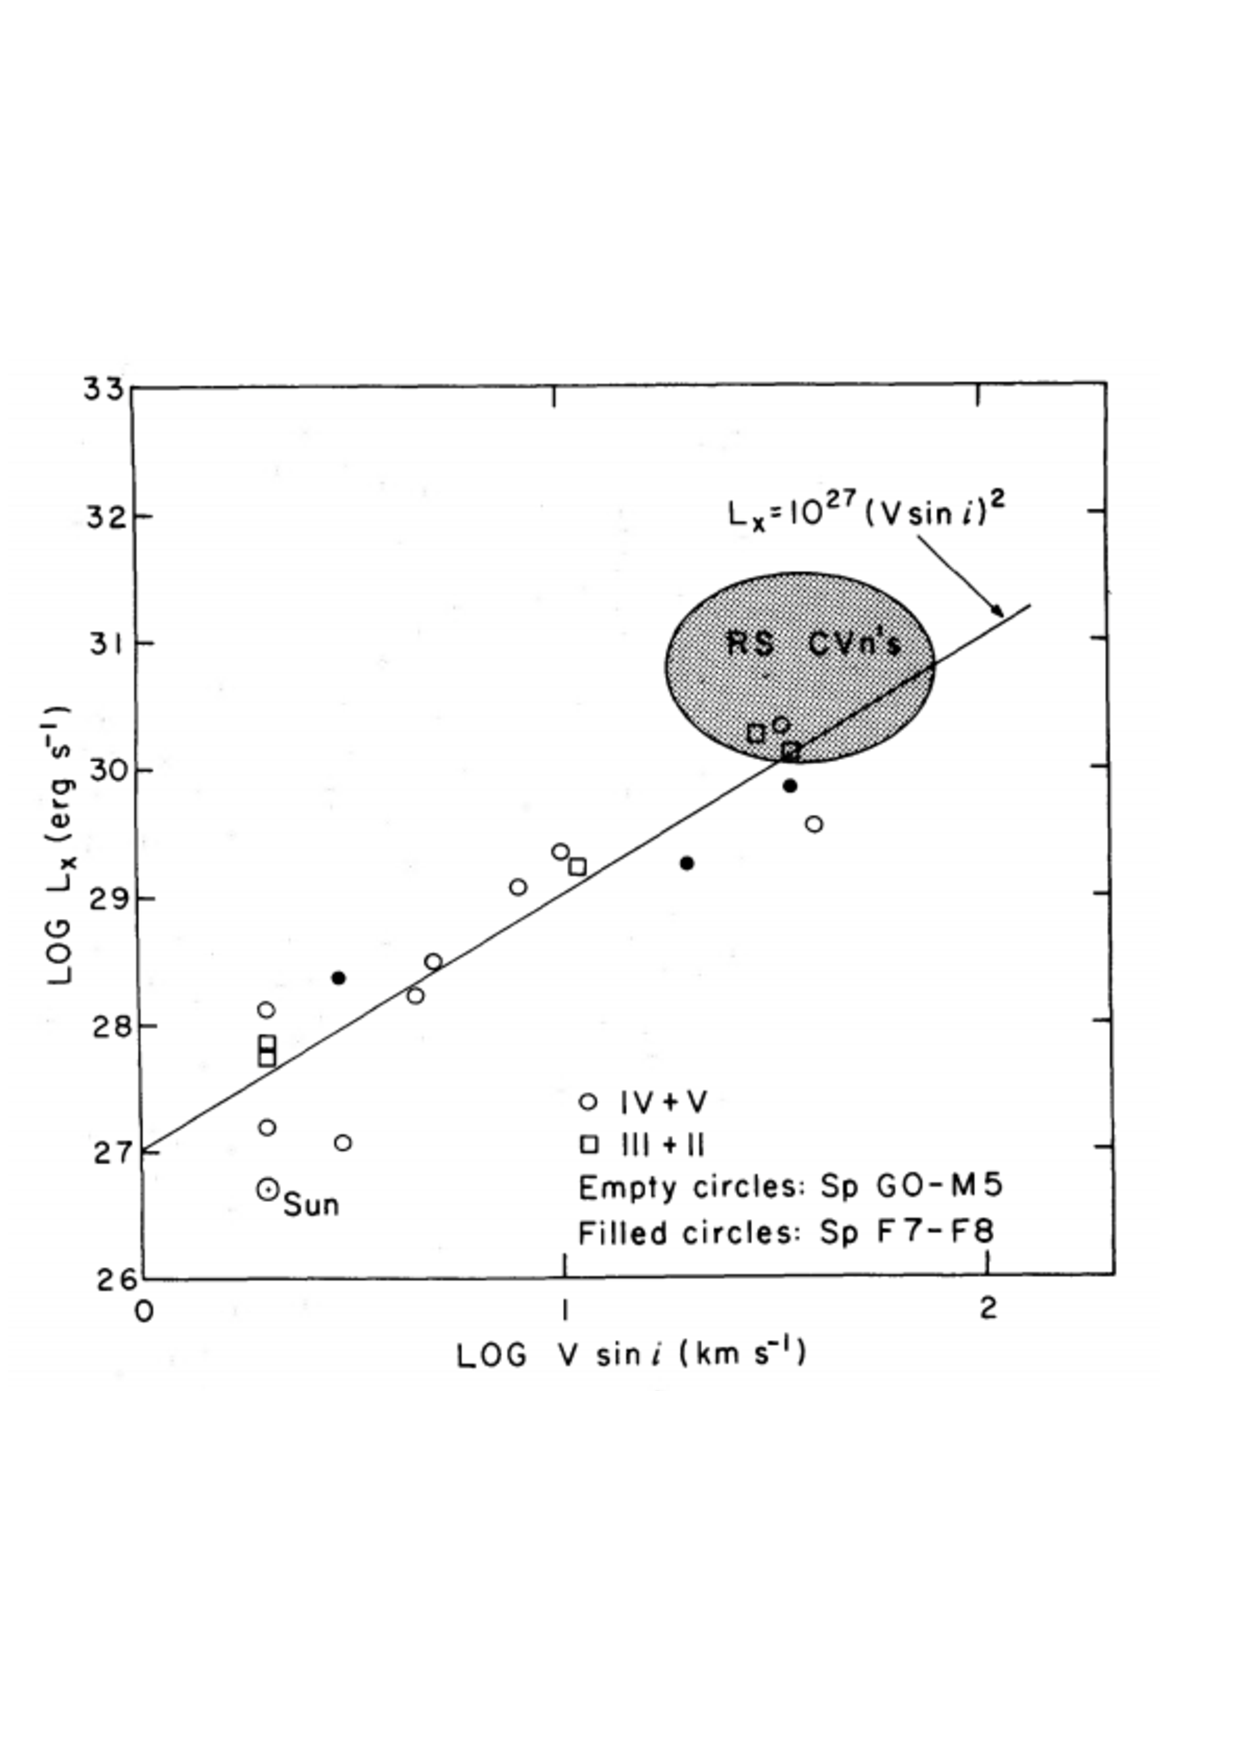
\includegraphics[scale=0.5]{Figures/2-Historical_overview/p81_fig_5.pdf}
    \caption[First plot of magnetic activity as a function of rotational velocity]{X-ray luminosity as a function of rotational velocities for a sample of G-M stars. Image credit: \citet{Pallavicini_etal_1981}}
    \label{fig:pallavicini_etal_1981_plot}
\end{figure}

\begin{equation}
    L_{x} \sim 1.4\text{x}10^{27}(v\sin i)^{1.9 \pm 0.5}
    \label{Eq:pallavicini_81}
\end{equation}

\citet{Noyes_etal_1984} were the first to plot a magnetic activity indicator (in this case the chromospheric emission \Rprime) as a function of the Rossby number. For their sample, rotation periods were inferred from the period modulation of the S index of Mount Wilson stars. This was an improvement on the rotational parameter used by \citet{Pallavicini_etal_1981} since it was dependent on the inclination of the star. \citet{Noyes_etal_1984} found that there was less scatter in the data if \Rprime was plotted as a function of Rossby number in comparison to plotting it as a function of simply rotation period. This suggested that the mean level of chromospheric activity is governed by a single parameter, the Rossby number and that the Rossby number is a major determinant of magnetic field amplification in convecting and rotating stars.

\citet{Pizzolato_etal_2003} considered a sample of 259 stars, consisting of 110 field star and 149 members of clusters ranging in (B-V) colour from 0.5 - 2.0. All of the X-ray observations were taken from ROSAT and the majority of the sample had photometric observations of the rotation period. Figure \ref{fig:pizzolato_etal_2003_plot} shows the X-ray luminosity as a function of the empirically derived Rossby number ($R_{e}$) for the whole sample of stars. This plot clearly shows both the saturated and unsaturated regimes of the activity-rotation relation. The saturated regime shows that for the fastest rotators there is maximum X-ray luminosity that is reached ($\frac{L_{x}}{L_{bol}} \approx -3$). This is interpreted as the star having no more available surface area to accommodate more active regions \citep{Jardine_Unruh_1999}. In the unsaturated regime, the best fitting relationship found was $\frac{L_{x}}{L_{bol}} \propto R_{e}^{-2}$, which is in agreement with the \citet{Pallavicini_etal_1981} result. The study by \citet{Pizzolato_etal_2003} confirmed that a single relationship between X-ray luminosity and Rossby number can be obtained for solar and late-type stars and included stars less than $0.5 M_{\odot}$ for the first time.

\begin{figure}
    \centering
    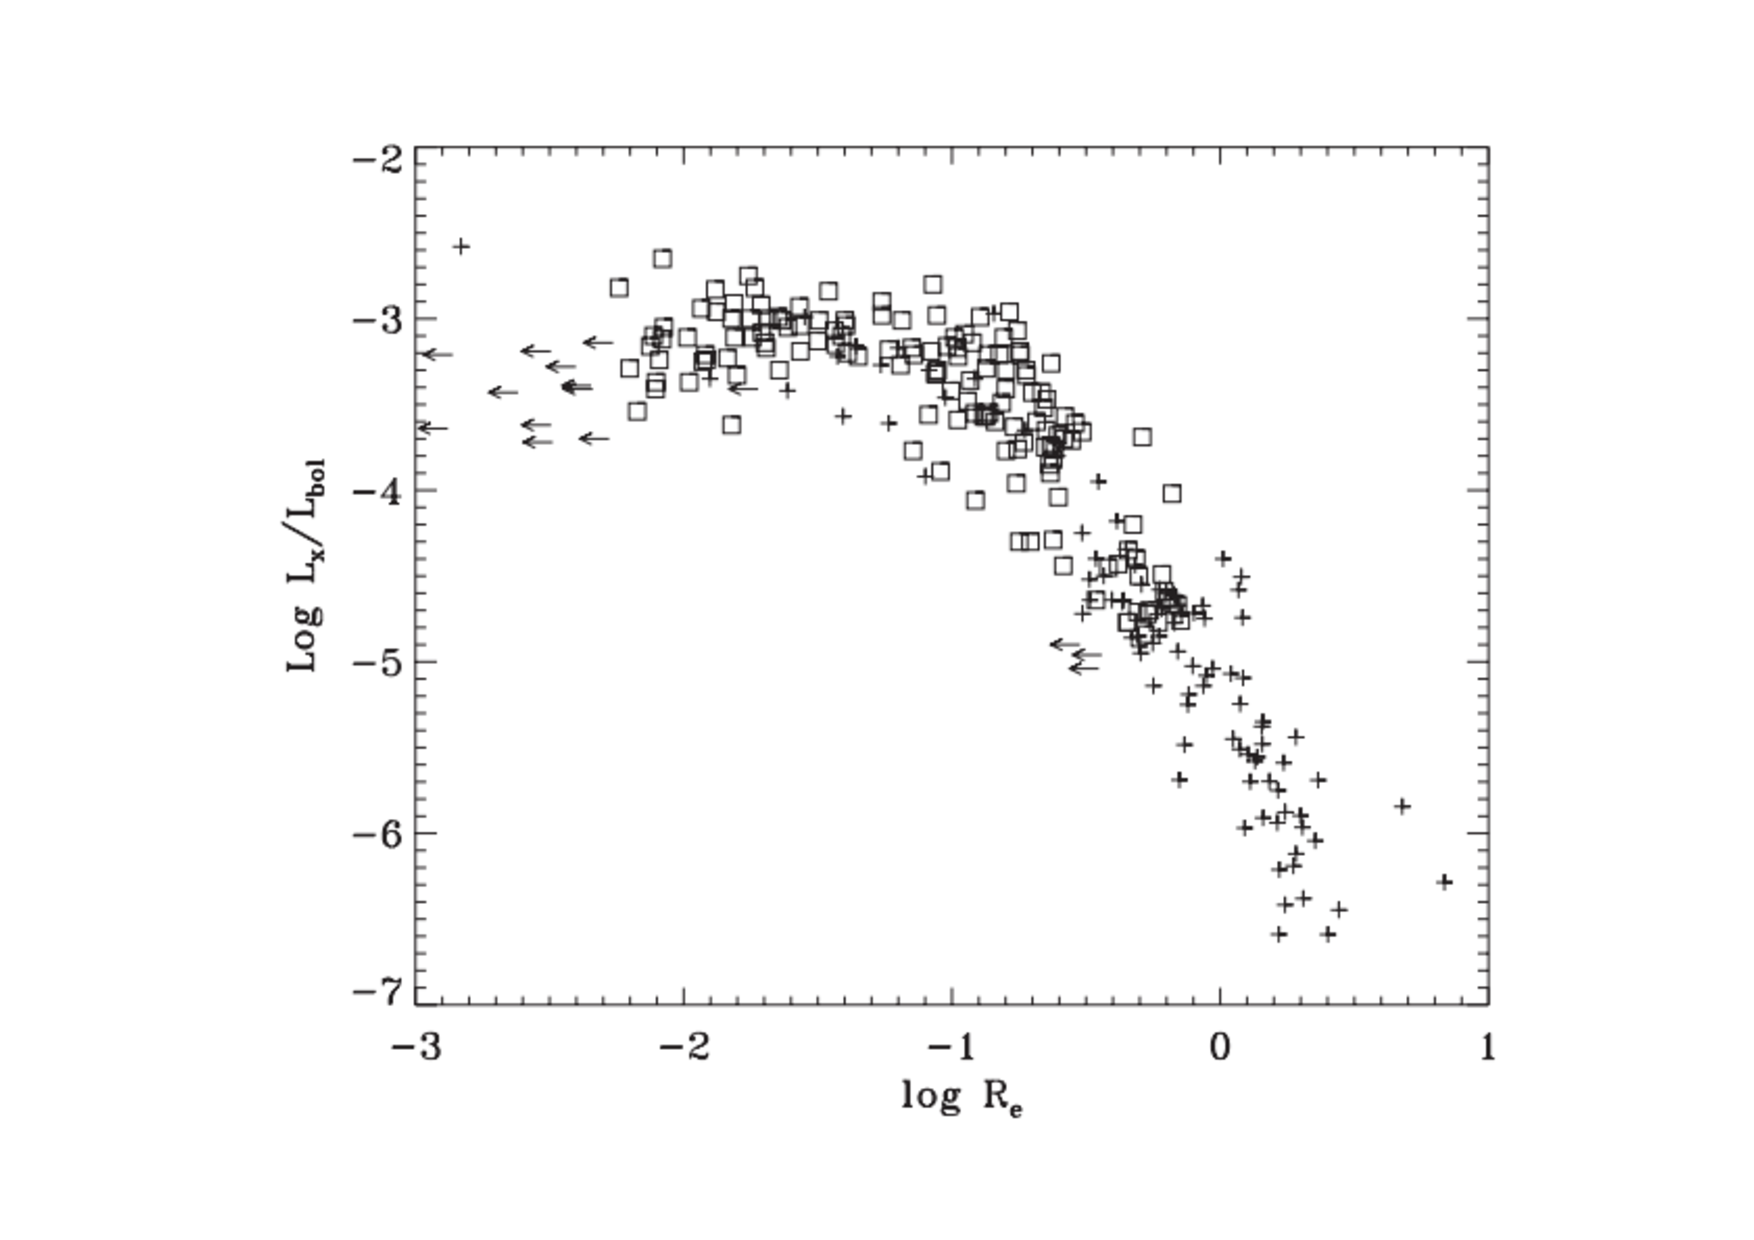
\includegraphics[scale=0.55]{Figures/2-Historical_overview/p03_fig_9.pdf}
    \caption[Activity-rotation relationship from \citet{Pizzolato_etal_2003}]{Ratio of X-ray to bolometric luminosity as a function the empirically derived x-ray Rossby number for the \citet{Pizzolato_etal_2003} sample of stars. $v\sin i$ measurements are denoted by arrows. Image credit: \citet{Pizzolato_etal_2003}}
    \label{fig:pizzolato_etal_2003_plot}
\end{figure}

A later study of the activity-rotation relationship was conducted by \citet{Wright_etal_2011} which has a much bigger sample of 824 solar and late-type stars with X-ray luminosity and rotation periods. The goals of this paper were similar to that of \citet{Pizzolato_etal_2003}, namely to study the activity-rotation relationship and derive a new estimate of the convective turnover time. In this study they define the parameter $R_{x}$, which is simply the ratio of X-ray to bolometric luminosity. When considering their whole sample, they find a relationship between activity and rotation of the form: $R_{x} \propto R_{0}^{-2.18}$, which is slightly steeper than the canonical value of -2 seen in previous studies \citep{Pallavicini_etal_1981,Pizzolato_etal_2003}.

\begin{figure}[h]
    \centering
    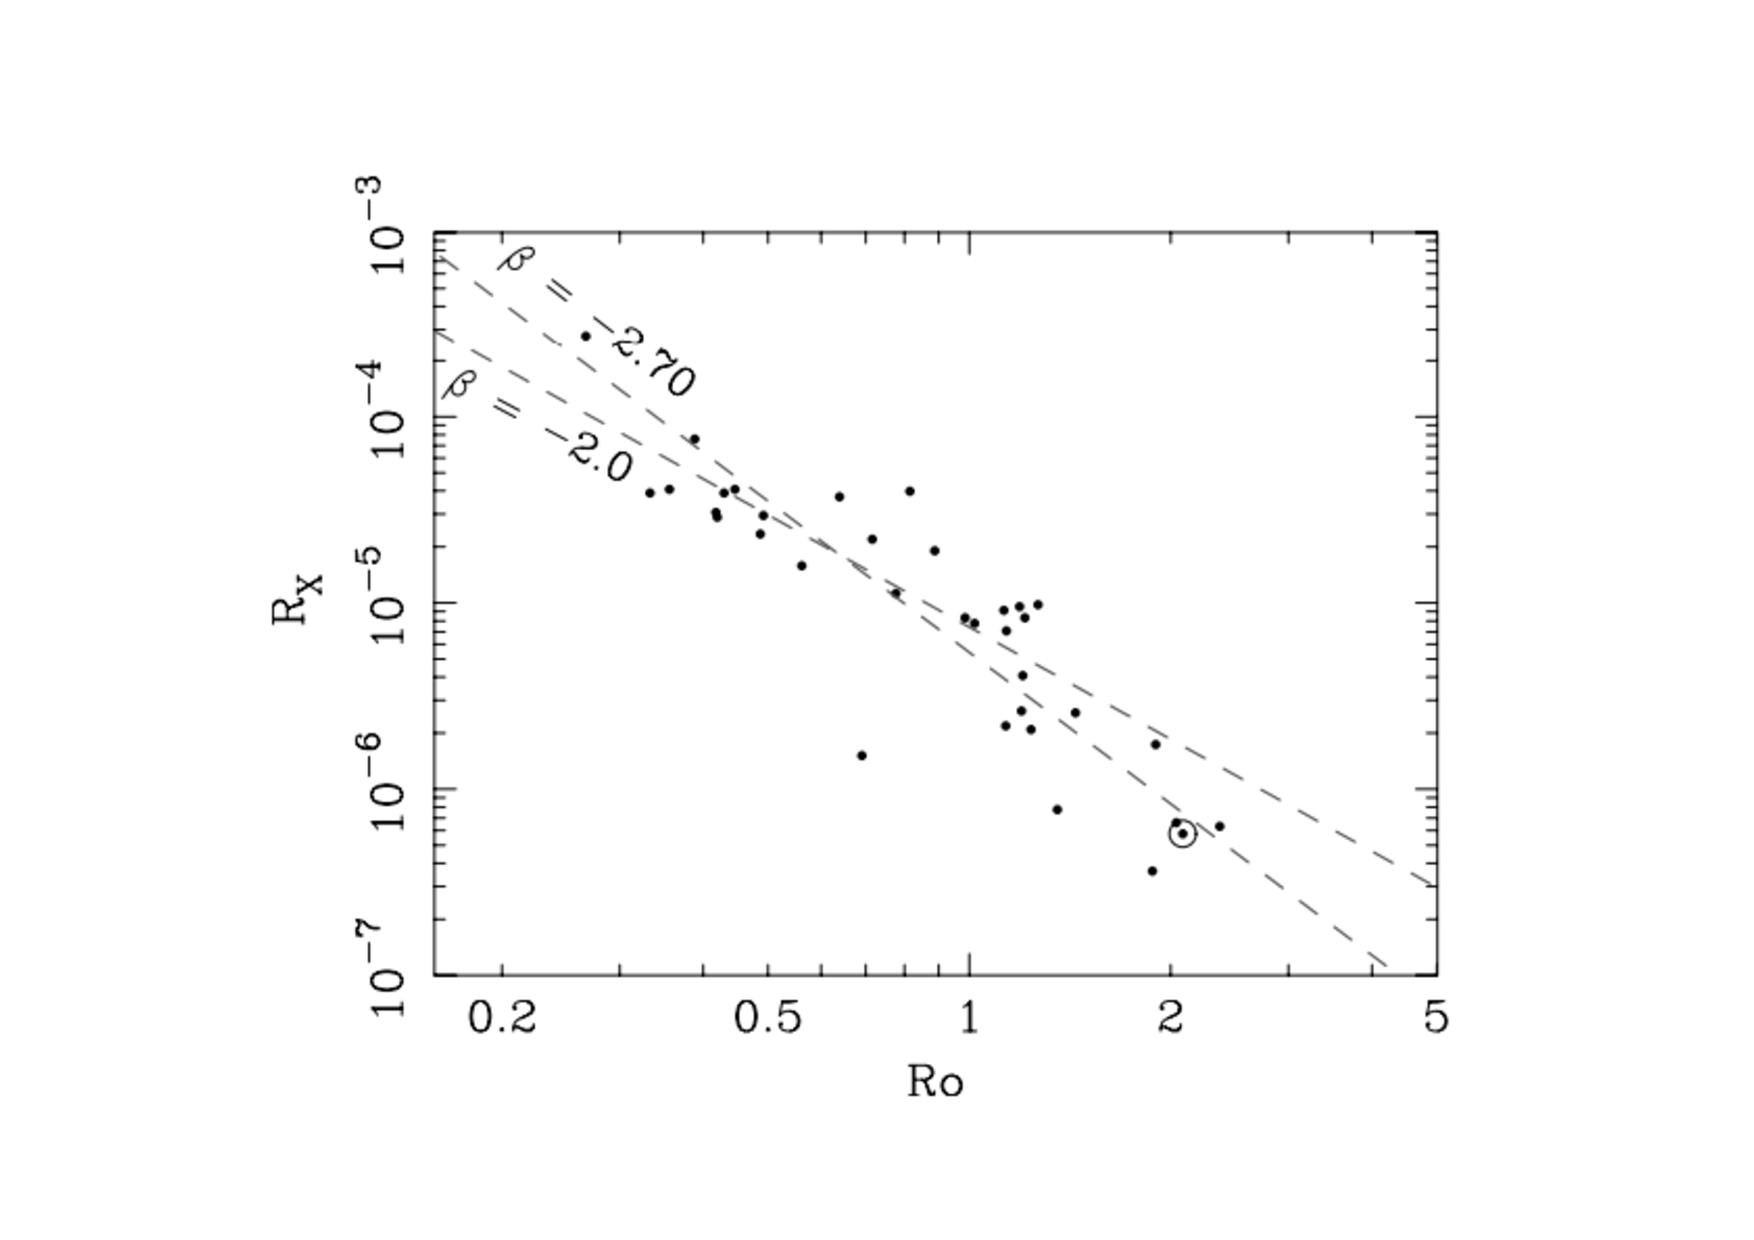
\includegraphics[scale=0.55]{Figures/2-Historical_overview/wright_etal_fig_3.pdf}
    \caption[Activity-rotation relationship for small, unbiased subset of \citet{Wright_etal_2011} data]{Small sample from \citet{Wright_etal_2011} that should be free from any detection bias in X-ray luminosity with $R_{x}$ plotted as a function of Rossby number. For this smaller sample, the best fitting relationship power law found has an exponent of $-2.70$, which is much steeper than the canonical value of $-2.0$. Image credit: \citet{Wright_etal_2011}}
    \label{fig:wright_etal_2011_plot}
\end{figure}

However, perhaps more importantly, they acknowledge that there are biases in their sample; at the largest $R_{0}$, it is likely that many of the faintest X-ray sources are not detected. Therefore they attempt to overcome these biases by compiling a smaller sample that should be unbiased. When they fit a power law to the smaller sample of 36 stars (as shown in Figure \ref{fig:wright_etal_2011_plot}), an exponent for the power law of $-2.70 \pm 0.13$ is found. This exponent value is much steeper than the value found for the whole sample but is in agreement with \citet{Gudel_etal_1997} and \citet{Feigelson_etal_2004} (which will be discussed in Section \ref{hist_xray_age_section}). This small, unbiased subset of data would suggest that there is a steepening of the activity-rotation relationship.

The most recent paper that concerned the activity-rotation relationship is by \citet{Metcalfe_etal_2016} which was motivated by the \citet{van_Saders_etal_2016} result and attempted to find a magnetic counterpart. The study compiled published values for the \Rprime indicator for the \citet{van_Saders_etal_2016} sample. They plotted the values found as a function of rotation period (seen in Figure \ref{fig:metcalfe_etal_2016_plot}) and compared their sample to G stars from the Mount Wilson survey. In \citet{Metcalfe_etal_2016}, a quantitative relationship is not fitted, however they do suggest that the Sun may be in a transitional evolutionary phase and may be a special case of stellar dynamo theory. They postulate that a change in the differential rotation is the underlying mechanism that disrupts the large scale organisation of magnetic field in solar-type stars and that at Rossby number of $\approx 2.0$, a shift in the magnetic topology causes the magnetic braking to operate with reduced efficiency. It is worth noting that the previous activity-rotation relationships all used the X-ray luminosity as the magnetic activity indicator and \citet{Metcalfe_etal_2016} is one of a few to study the chromospheric emission.

\begin{figure}
    \centering
    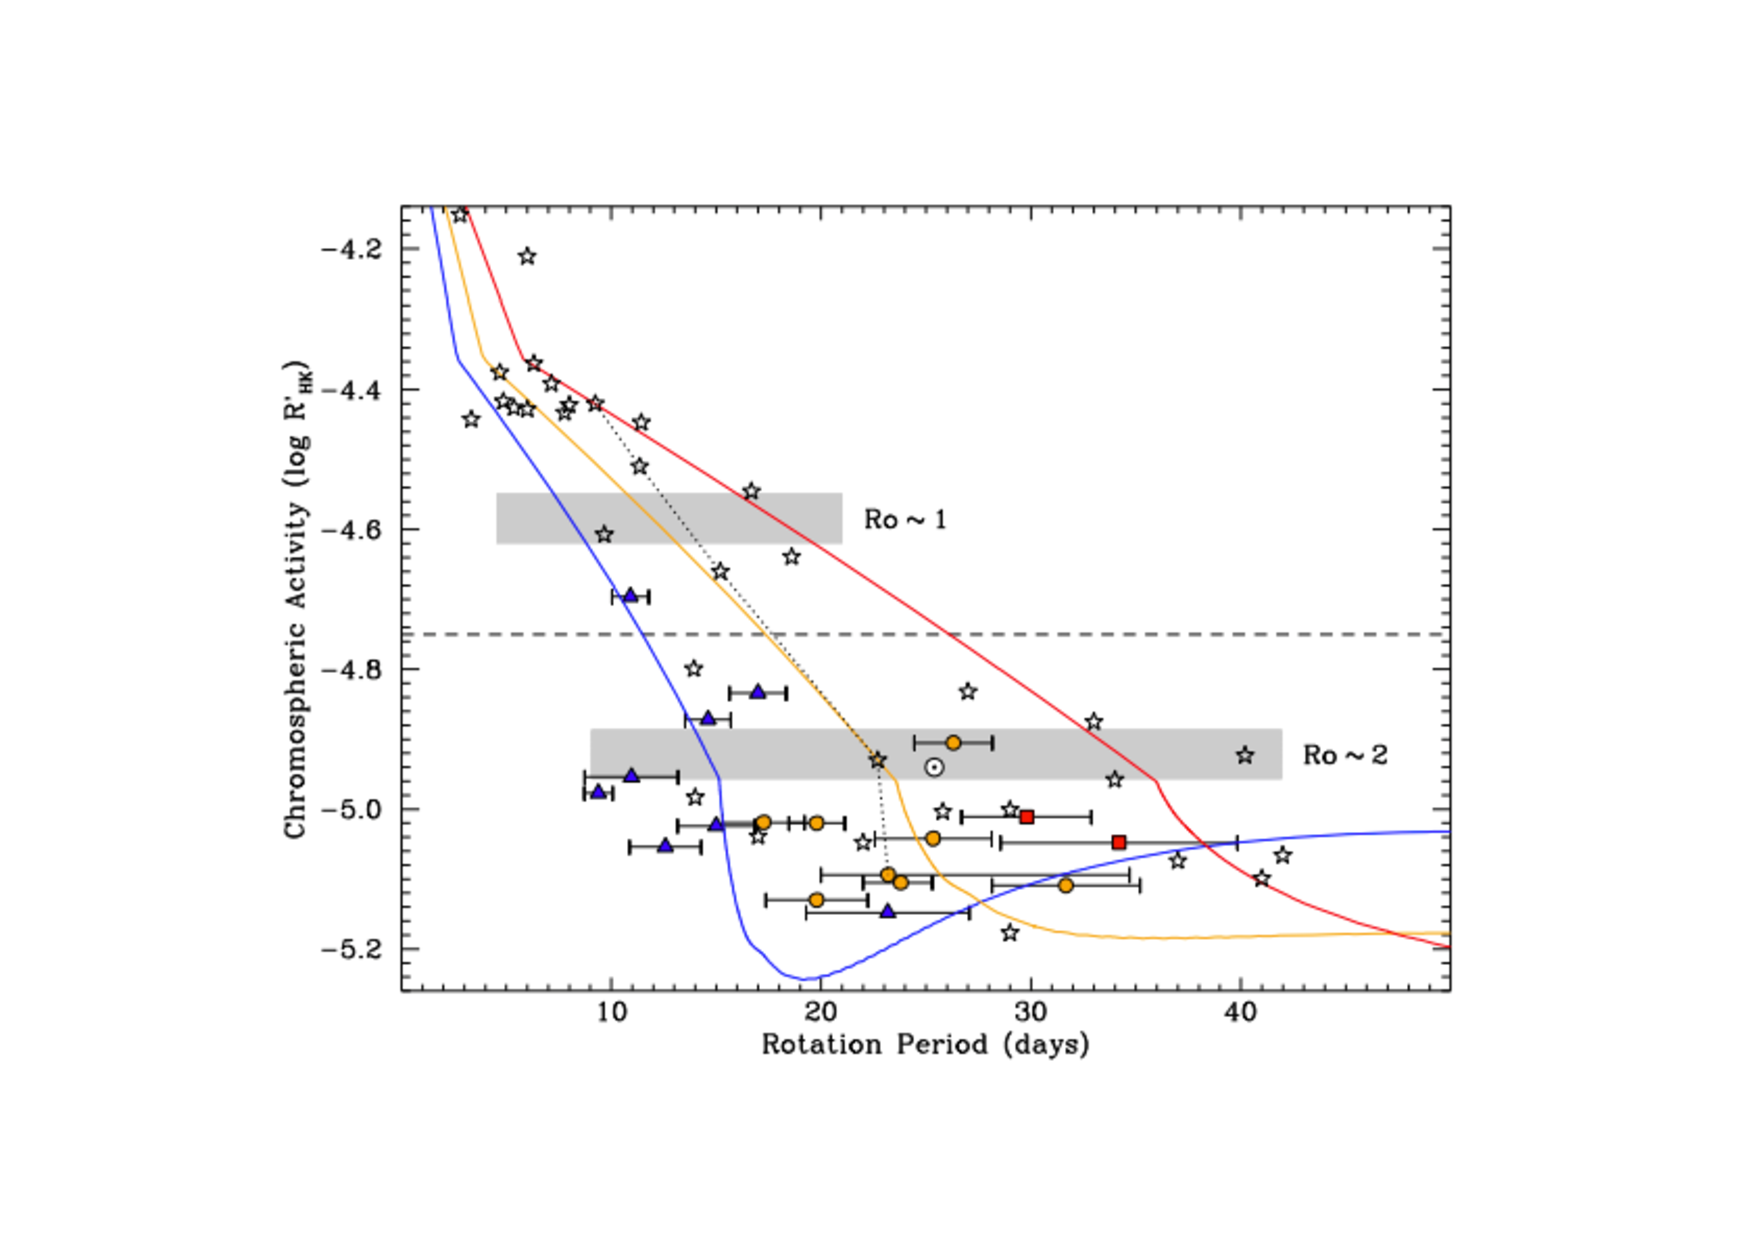
\includegraphics[scale=0.5]{Figures/2-Historical_overview/metcalfe_etal_2016_fig1.pdf}
    \caption[Chromospheric emission as a function of rotation period for sample of older stars]{Sample of stars from \citet{Metcalfe_etal_2016} with the \Rprime indicator plotted as a function of rotation period. Stars from the Mount Wilson survey are shown as star symbols. Rotational evolution models from \citet{van_Saders_etal_2016} are shown as lines. Image credit: \citet{Metcalfe_etal_2016}}
    \label{fig:metcalfe_etal_2016_plot}
\end{figure}

\section{Activity-age studies}
\label{Chp2_section_activity_age}
\subsection{Chromospheric emission - age relationship}

After the seminal paper by \citet{Skumanich_1972}, the method in which calcium emission was measured was changed by \citet{Noyes_etal_1984} who introduced the \Rprime indicator (as discussed in Section \ref{chromospheric_emission_subsub}). This is now the standard method of measuring the calcium emission in stars. Further studies investigated the age-activity relationship through chromospheric emission in the calcium lines including the following studies.

%Soderblom etal 1991
\citet{Soderblom_etal_1991} investigated the calcium emission - age relationship to determine firstly its existence as there was still debate at that time in the literature to whether the relationship was statistical or deterministic. Secondly, they also wanted to determine the nature of the relationship and expand on the three data points shown by \citet{Skumanich_1972}. Their sample of stars was compiled from several sources; the first being stars from clusters as these ages are well known through isochrone methods, but they also recognise that there are few clusters that were observable and older than the Hyades. The second source is stars in binary systems who have an evolved companion as the ages of these could be obtained through Str\"{o}mgren photometry. \citet{Soderblom_etal_1991} also included some evolved, single F dwarfs with known ages and stars whose relative age was known, for example, kinematic information placing stars within the old disk or halo populations.

From this sample of stars with ages and calcium emission they found that there was a deterministic relationship between the two parameters that followed this relationship - $R^{'}_{HK} \propto t^{-\frac{2}{3}}$. However, a problem arose when this power law was used to calculate ages for nearby solar-type stars; it was not consistent with a constant star formation rate, the ages calculated from this power law suggested that there was an excess of young stars ( $t < 1$ Gyr) in the solar neighbourhood. Therefore \citet{Soderblom_etal_1991} also computed a fit that was consistent with constant star formation rate and added a cubic dependence between the two parameters for stars younger than the solar age.

%Lachaume etal 1999
Another study in the literature concerning the calcium emission - age relationship was conducted by \citet{Lachaume_etal_1999} who aimed to calculate ages for a sample of stars using five different methods. They calibrated their calcium emission - age relationship using their sample of stars and the "best" age chosen from isochrone, metallicity or rotation. \citet{Lachaume_etal_1999} plotted these ages against literature values for the \Rprime indicator but found that the majority of the scatter was due to stars with $B - V$ values less than 0.6 therefore they exclude these stars from their sample. The calcium emission - age relationship they calibrate shows a decrease with age which then flattens when $log(R^{'}_{HK}) < -4.8$. Note that this relationship is not entirely independent as some ages have been taken from rotation measurements.

%MH08
Another important study was carried out by \citet{Mamajek_Hillenbrand_2008} (hereafter MH08) which compiled a large sample of solar-type dwarfs within the colour range of $0.5 < (B-V)_{0} < 0.9$. This study included an investigation of each of the components of the age-activity-rotation relation and populated the young end of the relationship for the first time. Their sample contained 167 main sequence and pre-main sequence stars taken from clusters and binary systems in the field with isochronal ages. They explored the age-activity relationship by plotting the mean value of the \Rprime indicator (as shown in Figure \ref{fig:MH08_age_activity_plot}) and found a quadratic fit was most appropriate in the range of their sample - $-5.1 < \log R^{'}_{HK} < -4.0$ and $6.7 < \log\tau < 9.9$ where $\tau$ is the stellar age in years. However, when inverting the relationship to have an expression in terms of stellar age, it was more accurate to have a trinomal function as shown in Equation \ref{Eq:MH_08_trinomal_eq}.

\begin{equation}
    \log R^{'}_{HK} = 8.94 - 4.849\log\tau + 0.624(\log\tau)^{2} - 0.028(\log\tau)^{3}
    \label{Eq:MH_08_trinomal_eq}
\end{equation}

\begin{figure}
    \centering
    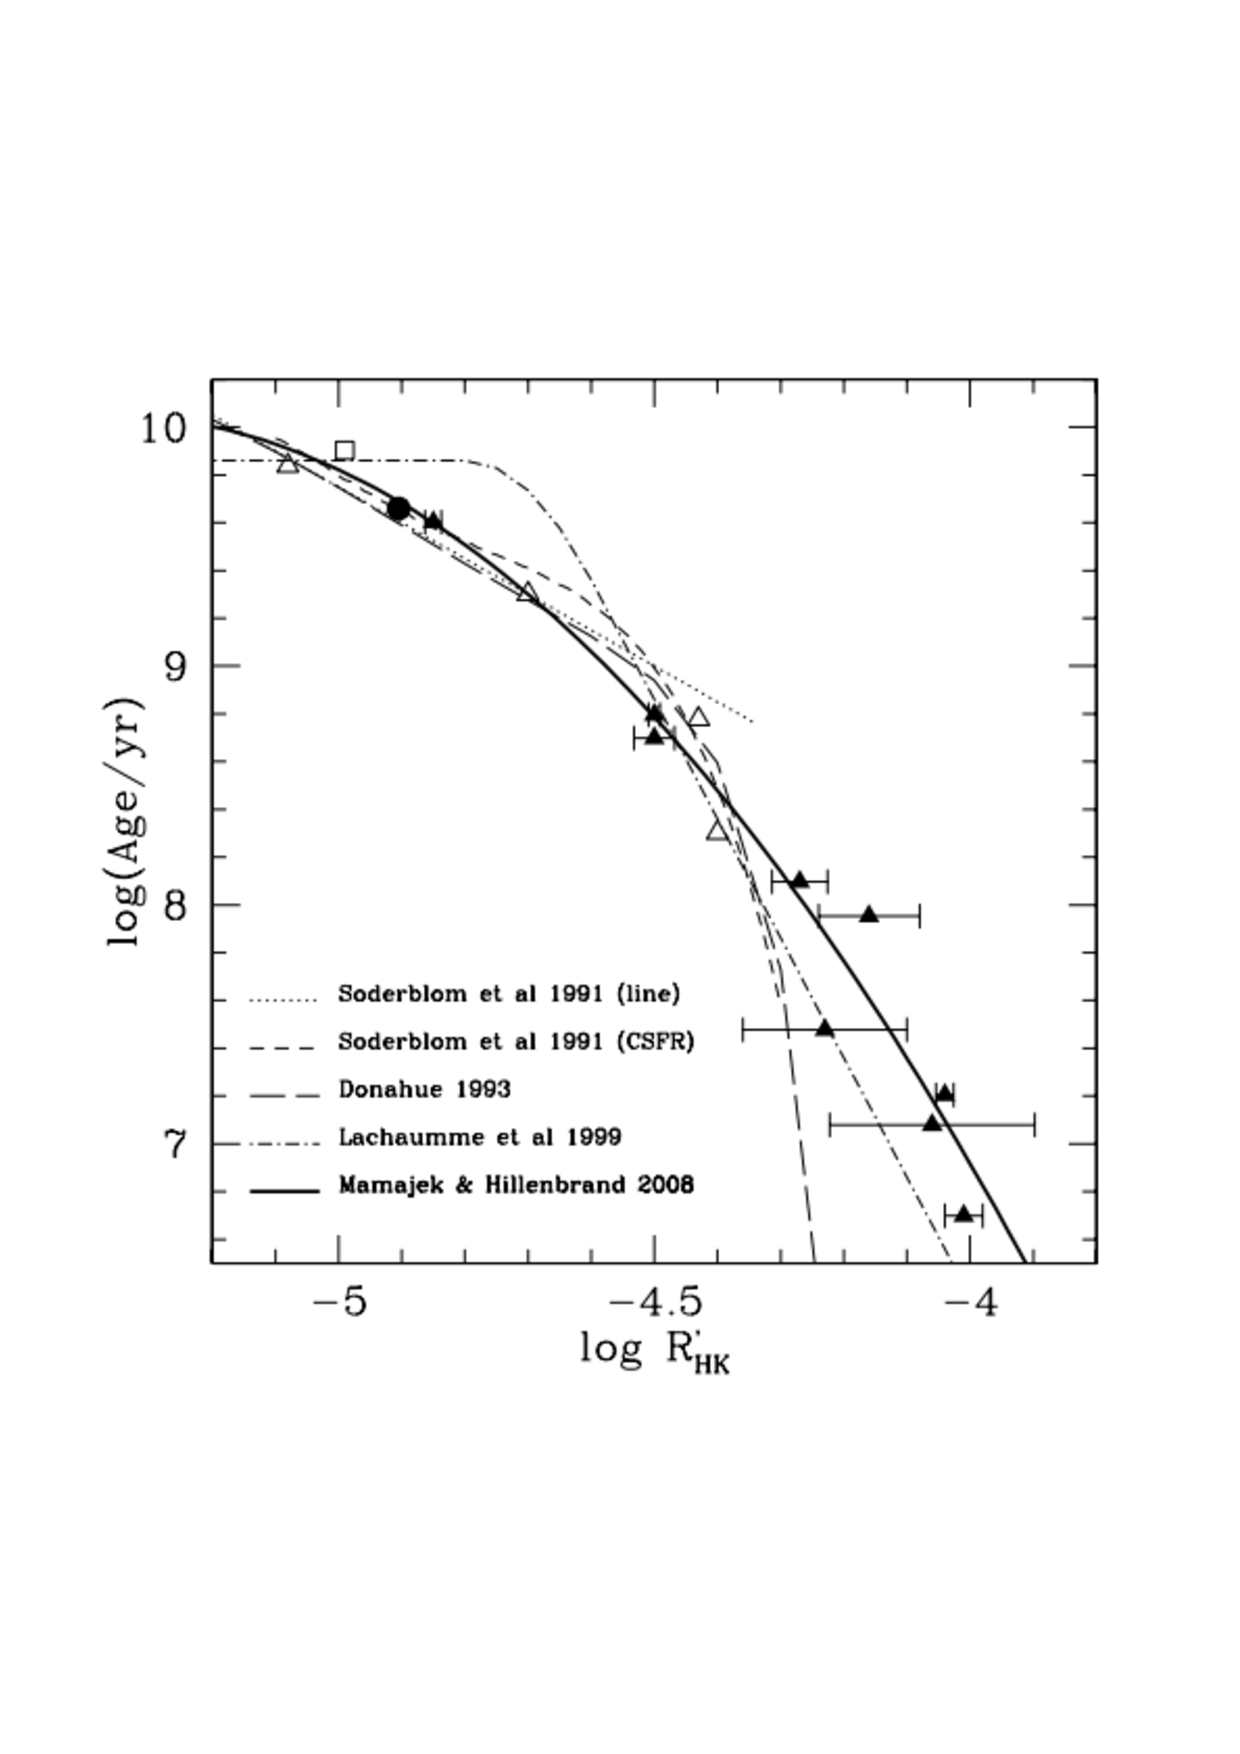
\includegraphics[scale=0.45]{Figures/2-Historical_overview/MH08_age_activity.pdf}
    \caption[Age-activity plot from \citet{Mamajek_Hillenbrand_2008} using chromospheric emission]{Age-activity plot from \citet{Mamajek_Hillenbrand_2008} that shows the \Rprime activity indicator as a function of stellar age for their sample. Previous age-activity relationships are plotted for reference in addition to their best fitting relationship. Image credit: \citet{Mamajek_Hillenbrand_2008}}
    \label{fig:MH08_age_activity_plot}
\end{figure}

Rotation periods were obtained for some of the MH08 sample, therefore the activity-rotation relationship was also investigated. The \Rprime indicator was plotted as a function of Rossby number  and three activity regions were found. For very active stars ($\log R^{'}_{HK} > -4.3$) little correlation was found between the two parameters, which is unsurprising as for very young stars there is a saturation of magnetic activity as seen in X-ray studies (e.g. \citealt{Jackson_etal_2012}). In the active regime ($-5.0 < \log R^{'}_{HK} < -4.3$), a very strong anti-correlation is found with Pearson coefficient (r) of -0.94. Lastly, in the inactive regime ($\log R^{'}_{HK} < -5.0$), very weak correlation is observed; note this is based on a small number of data points that seem to have a fairly large spread in Rossby number. From these rotation periods the study was also able to update the coefficients for the \citet{Barnes_2007} gyrochronology relationship.

MH08 also investigated the \Rprime indicator as a function of colour among binaries and kinematic groups to see if there is a mass dependency as these systems can be assumed to be the same age but different masses. For the 24 binary pairs a range of slopes between the \Rprime indicator and colour were found, both positive and negative. For a similar plot of the \Rprime indicator and colour for the kinematic groups there were no unique slopes applicable to all activity levels. In this plot, younger groups such as the Pleiades showed steep positive slopes which were $\approx 2\sigma$ steeper than the slope for Hyades. The oldest cluster displayed the most negative slope which may suggest that the slope ($\Delta\log R^{'}_{HK} / \Delta(B- V)$) may flatten as a function of age.

%Pace 2013
\citet{Pace_2013} called the age-activity relationship into question, particularly when using chromospheric emission from the \caII spectral lines. There was some evidence from open clusters that the chromospheric activity in stars with ages of 1.5 Gyr had similar activity levels to the solar value \citep{Pace_Pasquini_2004}. Therefore this study aimed to calibrate the age activity relationship, particularly for ages older than one gigayear. This was achieved by considering field stars with literature values for the \Rprime indicator and isochronal ages from the Geneva-Copenhagen survey of solar neighbourhood (GCS). Only stars with sufficiently precise ages were selected for the study, errors on the age had to be less than 2 Gyr.

The \Rprime indicator was plotted for the final sample of 1744 field dwarfs as a function of their stellar age as shown in Figure \ref{fig:pace_2013_plot}. This plot shows an L-shaped age-activity relationship which seems to suggest that the decay of chromospheric activity stops a a relatively young age. The age at which the chromospheric activity seems to stop its evolution is approximately 3 Gyr from the sample of field stars, however, due to the errors associated with the stellar age it may actually stop sooner than this. It is also worth noting that as the age of sample increases, the effective temperature of the stars in the sample decreases thus indicating that there may be biases in the sample. If the evolution of the chromospheric activity does indeed stop at a relatively early age then this would hinder the use of the parameter as an age indicator.

\citet{Pace_2013} also considered a sample of open clusters and found that there was a difference in the trend of the \Rprime indicator as a function of effective temperature depending on whether it was an active or inactive cluster. Young clusters tended to have a slight increase of the \Rprime with decreasing effective temperature. Older clusters had a more complicated pattern of the \Rprime indicator with effective temperature. The difference in age between the oldest active cluster and youngest inactive cluster was just 50 Myr. This was suggested to be due to a sudden drop in chromospheric activity however there was some doubt over the dependency of the oldest active cluster.

\begin{figure}
    \centering
    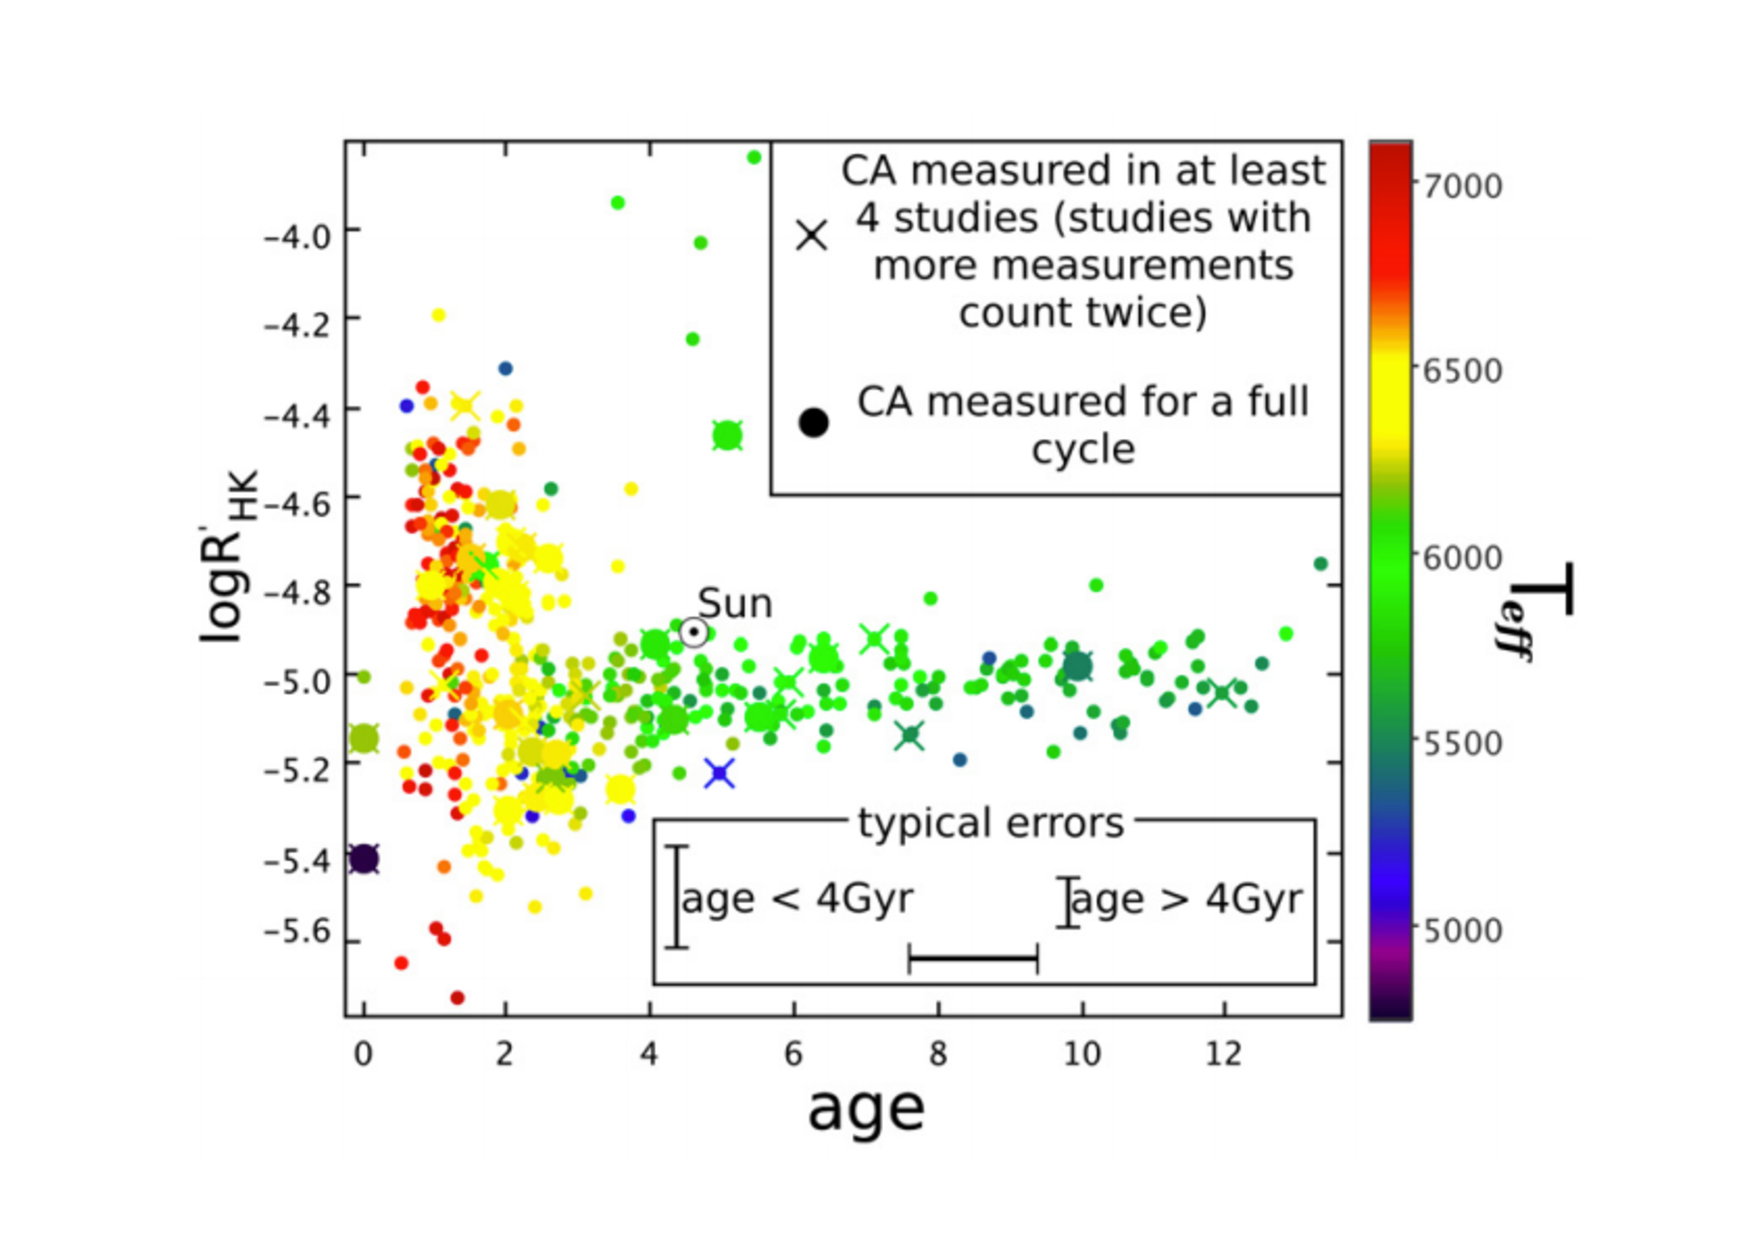
\includegraphics[scale=0.4]{Figures/2-Historical_overview/pace_2013.pdf}
    \caption[\citet{Pace_2013} age-activity relationship]{\citet{Pace_2013} plot of calcium chromospheric emission as a function of stellar age for the sample of field dwarfs with isochronal ages. Data points are coloured according to their effective temperature. Image credit: \citet{Pace_2013}}
    \label{fig:pace_2013_plot}
\end{figure}

%LO_etal_2016 (AMMAR)
While the age-activity relationship was called into question by \citet{Pace_2013}, this lead others to consider the potential issues with using the \Rprime indicator as an activity indicator. The work by \citet{Lorenzo_Oliveira_etal_2016} is an example of such a study, they analysed the presence of mass and metallicity biases that are implicit in conventional methods of selecting solar-type stars with precise isochronal ages such as the method in \citet{Pace_2013}. They argue that in order to obtain precise isochronal ages, most stars will be more massive than the Sun as a sizeable detachment from the ZAMS is needed to calculate a reliable age. Furthermore, such a sample will have a large range of metallicities and due to the age-metallicity relationship younger stars tend to be more metal rich. This has consequences for the chromospheric activity measured in these stars as they have deeper \caII profiles thus mimicking more subdued chromospheric activity. Younger stars in these types of samples also tend to be more massive (due to the necessary detachment from ZAMS for a reliable age), such stars have a decreased convective efficiency and will appear less active. Both of these selection effects combine to lower the chromospheric activity of the younger population of a sample. Conversely, older stars tend to be less massive and appear more active to to an increase in their convective efficiency. These older stars also tend to be metal-poor which will lead to shallower \caII profiles and mimic higher levels of chromospheric activity. The net result of such biases in a large sample will blur the range of the \Rprime indicator between young and old stars thus masking the true structure of the age-activity relationship.

In order to study this in more detail \citet{Lorenzo_Oliveira_etal_2016} collected a sample of field stars and open cluster members and derived an age-mass-metallicity-activity relation (hereafter AMMAR). They compared chromospheric ages from the MH08 relationship and their AMMAR to asteroseismic ages. The chromospheric ages calculated from their AMMAR showed excellent agreement with the asteroseismic ages. However, the chromospheric ages from the MH08 relation showed a trend in the difference between it and the asteroseismic age with metallicity. This further confirmed that the metallicity of a star can affect the chromospheric emission measured in \caII spectral lines and that it should be accounted for.

\citet{Lorenzo_Oliveira_etal_2016} were also able to reproduce the L-shaped age-activity relationship shown in \citet{Pace_2013} by selecting stars from GCS and using the same selection rules. They calculated the \Rprime indicator using their AMMAR and plotted the mean value and its dispersion as a function of age. They found that there was a constant metallicity dispersion ($\approx 2\sigma$) along the age domain which is understood to be an additional source of scatter in the age-activity relationship. Furthermore, the sample is increasingly bias towards higher masses at young ages which can also be seen in the plot from \citet{Pace_2013} in Figure \ref{fig:pace_2013_plot}.

%Lorenzo-Oliveira etal 2018
Considering the evidence of mass and metallicity effects on the \Rprime indicator, it seems that care must be taken when considering large sample of stars. In order to minimise these effects, careful selection criteria must be enforced to the sample. An example of such a study was undertaken by \citet{Lorenzo_Oliveira_etal_2018}, where they consider a sample of solar twins with isochronal ages. Spectroscopic binaries and stars in a binary systems with a companion closer than 4" were removed from sample as close companions may exchange angular momentum with the solar twin, therefore altering the evolution of the stellar angular momentum.

\begin{figure}
    \centering
    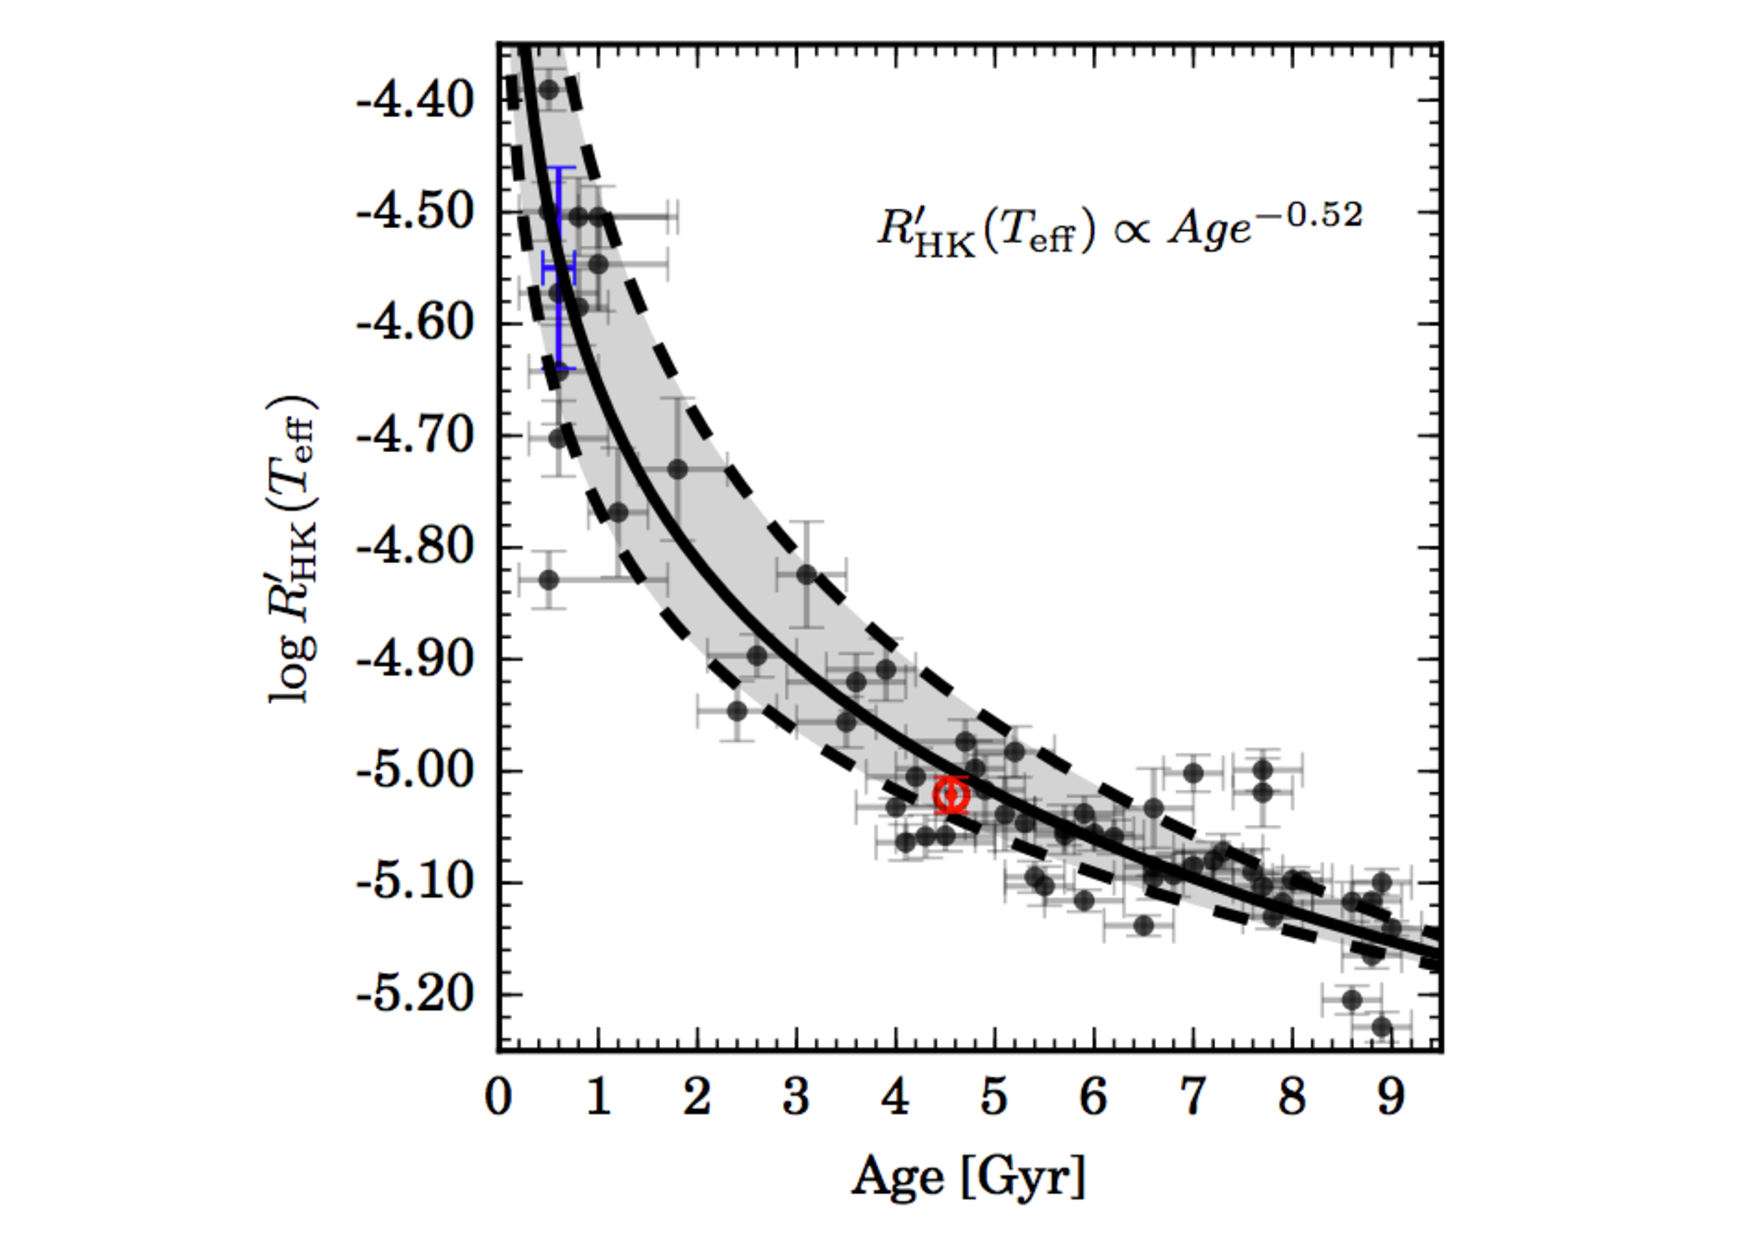
\includegraphics[scale=0.45]{Figures/2-Historical_overview/LO_etal_18_age_activity_plot.pdf}
    \caption[\Rprime - age relationship for sample of solar twins]{The \Rprime indicator (calibrated to effective temperature) plotted as a function of isochronal age for a sample of solar twins. The Sun is shown as a red symbol and stars younger than a gigayear are represented by a single cluster (blue data point). The black line is the best fitting relationship which is given by Equation \ref{Eq:LO_etal_18_law}. The shaded region is the 2$\sigma$ activity variability prediction band. Image credit: \citet{Lorenzo_Oliveira_etal_2018}}
    \label{fig:LO_etal_18_plot}
\end{figure}

The S index was calculated for each star using spectra from HARPS and calibrated to the Mount Wilson S index (\Smw). There are a number of reasons why the S index must be calibrated to the Mount Wilson index, firstly due to the calculation of the \Rprime indicator which is based off the Mount Wilson value. Secondly, the value of the S index is dependent on the throughput of the spectrometer thus in order to have consistent values for the S index it is transformed into the Mount Wilson value. Once the \Smw value had been determined for the sample, this could then be converted into the \Rprime indicator. However, \citet{Lorenzo_Oliveira_etal_2018} calibrated the correction factor $C_{cf}$ as a function of effective temperature and claimed to improve the method used to calculate the \Rprime indicator.

\citet{Lorenzo_Oliveira_etal_2018} plotted their \Rprime values (calibrated to effective temperature) as a function of the isochronal age which is shown in Figure \ref{fig:LO_etal_18_plot}. The best fitting relationship (Equation \ref{Eq:LO_etal_18_law} where Age is in Gyr) shows that for this sample of solar twins, the decay of magnetic activity with time is very close to that of the Skumanich Law. More importantly, it confirms that the age-activity relationship remains statistically significant after solar age for solar twins.

\begin{equation}
    R^{'}_{HK}(T_{eff}) \propto Age^{-0.52}
    \label{Eq:LO_etal_18_law}
\end{equation}

\subsection{Coronal activity - age relationship}
\label{hist_xray_age_section}
We know that magnetic activity is also displayed in the corona and that the X-ray luminosity is a good magnetic activity indicator. Therefore, it is no surprise that there have also been attempts to calibrate an age-activity relationship by using the X-ray luminosity as a magnetic activity indicator. One of the earliest attempts was by \citet{Maggio_etal_1987} who used a survey of late-F and G type stars from the Einstein telescope to investigate a volume-limited sample. As part of this investigation, they plotted the X-ray luminosity as a function of age. Note that the ages used in this study were either cluster ages or individual ages based on lithium abundances. They found that their sample followed a relationship of the form: $L_{x} \propto t^{-1.5}$. However, this did include upper limits for X-ray luminosities and lower boundaries for stellar ages.

%Gudel etal 1997
A later study by \citet{Gudel_etal_1997} investigated the dependence of coronal temperature and emission measure on age and rotation period using a sample of nine solar-like G stars with ages from 70 Myr to 9 Gyr and data from the ASCA and ROSAT X-ray satellites. Previous X-ray studies had indicated that the corona of active stars tended to be hotter than low activity analogues \citep{Schmitt_etal_1995}. \citet{Gudel_etal_1997} confirm this with their sample of stars, finding a dependence between X-ray luminosity and the value of the hotter temperature component of the form: $L_{x} \propto T_{hot}^{4}$. this is interpreted as a decrease in the efficiency of the high temperature coronal heating mechanism as a function of age. Ages were also collected for their sample of G type stars from clusters/moving groups, rotational and isochronal ages. They found that the best fitting relationship between the X-ray luminosity and stellar age followed a power law with an exponent of $-1.5$, in agreement with the findings of \citet{Maggio_etal_1987}.

%Feigelson etal 2004
A different approach was taken by \citet{Feigelson_etal_2004} who utilised the Chandra deep field - North (CDF-N) which probes a region of the sky to a very low X-ray limit of $3 x 10^{-17}$ cm$^{-2}$ ergs s$^{-1}$ in the soft band (0.5 - 2 keV). \citet{Feigelson_etal_2004} used the $\approx$ 3\% of the sample that were low mass stars resulting in 11 stars. While individual ages were not known for these stars, limits to the ages could be determined. The stars in the sample were not sufficiently high above the galactic plane to be likely members of the thick disc or halo, both of which are known to be very old. Therefore, the stars in the sample must belong to the thin disk , thus setting an upper limit for their age of 11 $\pm$ 1 Gyr.

Instead of plotting X-ray luminosity as a function of age since individual ages were not available, the observed X-ray distribution of the sample was compared to predicted populations assuming different magnetic activity decay laws of the form: $L_{x} \propto t^{\alpha\beta}$ where $\alpha$ represents the exponent of the rotational spin-down law (Equation \ref{Eq:general_rotation_age}) and $\beta$ is the exponent of the activity-rotation law (Equation \ref{Eq:general_activity_rotation}). This approach was only feasible due to the nature of the CDF-N, it is complete in both X-ray population and the identification of stellar counterparts (within the flux limits). \citet{Feigelson_etal_2004} find that a value for the decay law exponent of $\alpha\beta = -2$ provides an excellent fit to the data but due to the small sample size and systematics they also cannot rule out an exponent value of $\alpha\beta = -1$ which is the expected value from other studies of rotation-age and activity-rotation relationships.

%Giardino etal 2008
\citet{Giardino_etal_2008} studied the X-ray luminosities for members of NGC 752, a 1.9 Gyr old cluster. Clusters with this approximate age are useful as they bridge the gap in between the Hyades and the Sun where most of the decrease in X-ray luminosity occurs. Seven data points for NGC 752 were obtained and plotted alongside data for other clusters and the Sun. The median X-ray luminosity of NGC 752 showed good agreement with the decay magnetic activity trend and was consistent with an exponent of $\alpha\beta \sim -1.5$. Again, these results are in agreement with \citet{Maggio_etal_1987} and \citet{Feigelson_etal_2004}.

%Jackson etal 2012
Probably the largest study of the X-ray luminosity-age relationship to date was conducted by \citet{Jackson_etal_2012} that studied a large sample of stars in open clusters. They selected 717 stars from 13 open clusters and aimed to study in particular the saturated regime of the activity-age relationship and the implications for exoplanets. Their sample had a (B-V) colour range of 0.29 to 1.41 which consists of F, G and K stars. Upper limit results for $L_{x}$, giant stars and flare stars were excluded from the analysis. The sample was filtered into colour bins as a proxy for mass since the decay of magnetic activity is expected to depend on this parameter.

\begin{figure}[t]
    \centering
    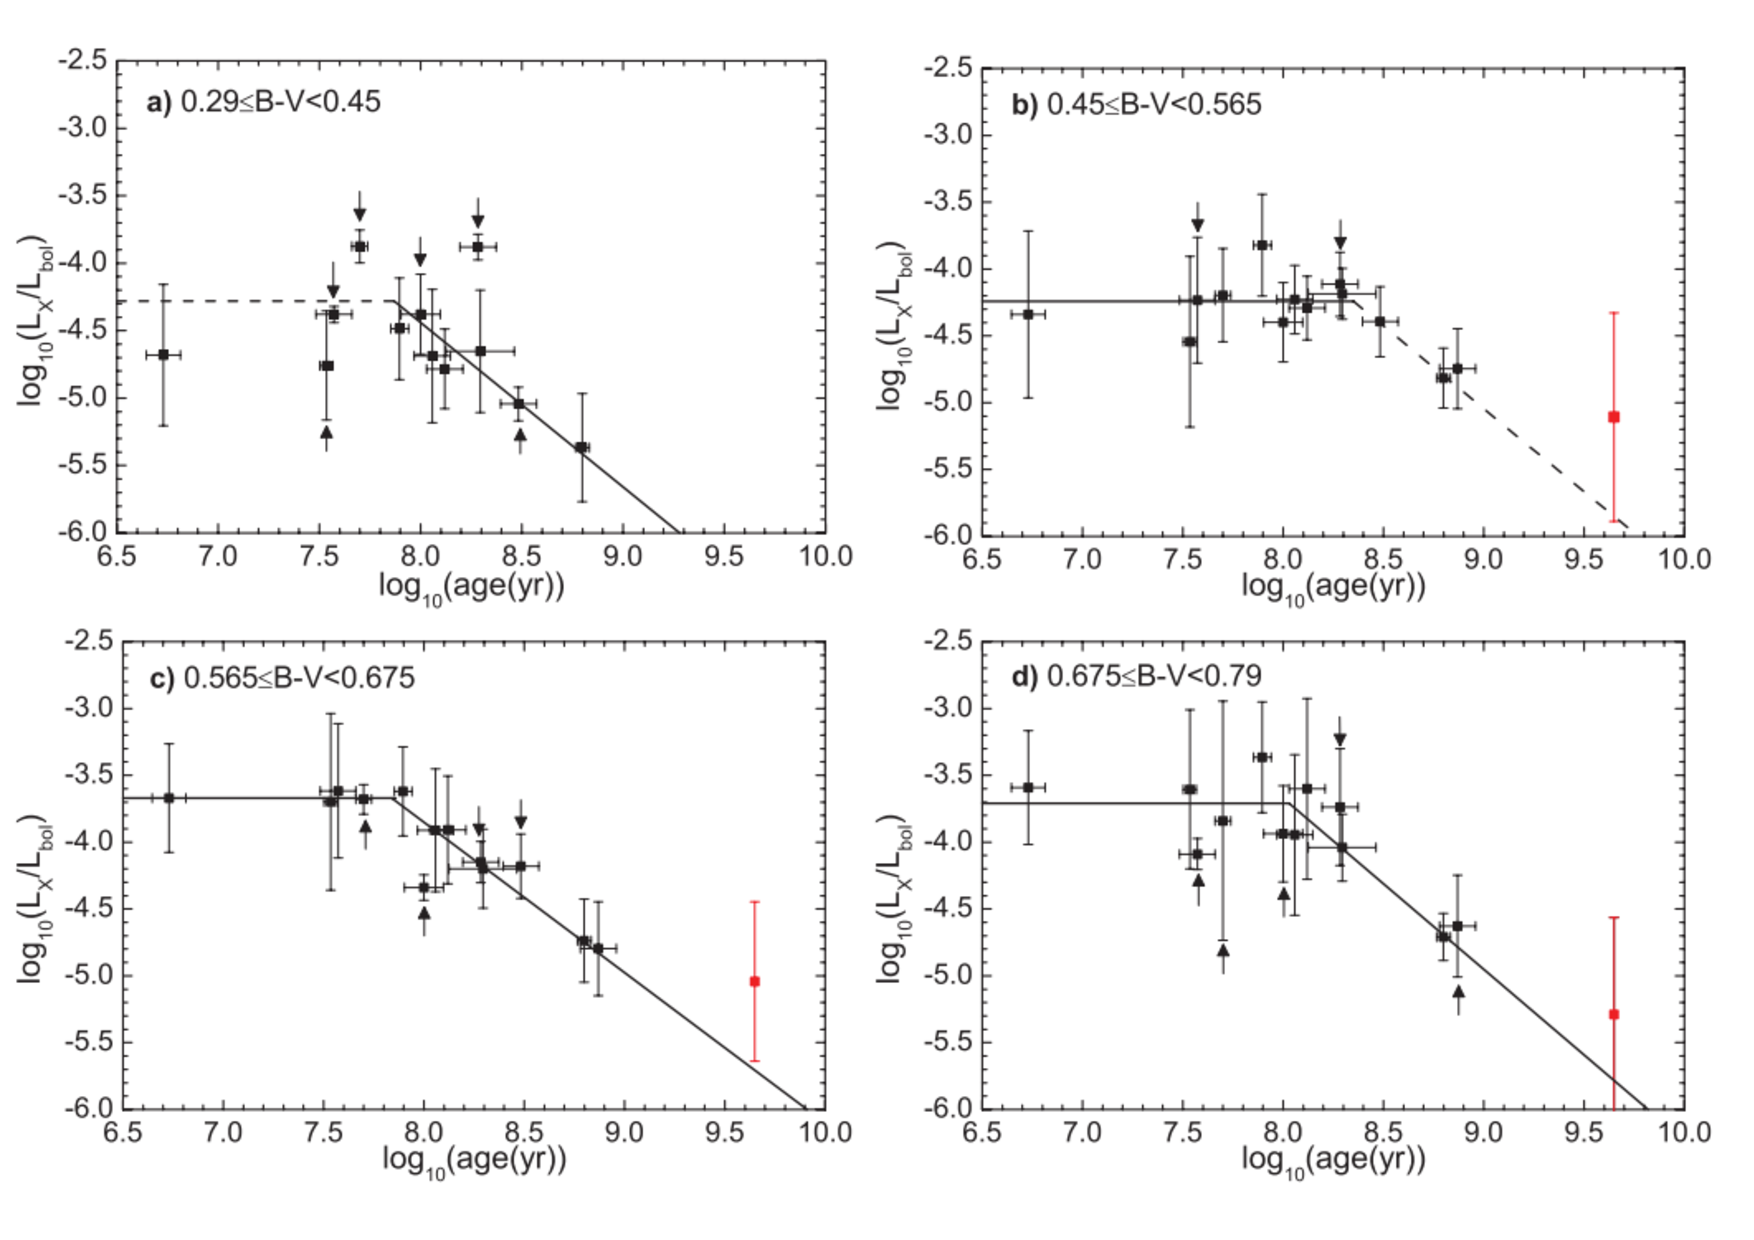
\includegraphics[scale=0.45]{Figures/2-Historical_overview/jackson_etal_2012_part.pdf}
    \caption[\citet{Jackson_etal_2012} X-ray luminosity - age relationship for sample of clusters]{Plot of X-ray luminosity as a function of stellar age for cluster data. Each subplot shows the relationship in a particular mass bin as defined by the (B-V) colour. Solid lines indicate best-fitting relationships, while dashed lines show more uncertain fits. Red data point indicates the field sample from \citet{Pizzolato_etal_2003} for reference. Image credit: \citet{Jackson_etal_2012}}
    \label{fig:jackson_etal_2012_plot}
\end{figure}

While the previous studies discussed concentrated on measuring the rate of decay of magnetic activity with time, this study also focused on measuring the saturated X-ray emission at very young ages. This is clearly seen in the activity-rotation relationships (see Section \ref{Chp2_activity-rotation_lit_review}), where at rotation periods shorter than $\sim 1-2$ days the trend of increasing X-ray luminosity with decreasing rotation period stops and the X-ray luminosity is constant for very fast rotators. At these extremely fast rotation rates, it is thought that the coronal emission is at the physical maximum, i.e. the star has no more available surface area to accommodate more active regions \citep{Jardine_Unruh_1999}.

In \citet{Jackson_etal_2012}, a broken power law was fitted to the cluster data in each (B-V) bin as shown in Figure \ref{fig:jackson_etal_2012_plot}. In the saturated regime, the gradient was constrained to be zero but in the unsaturated regime this was allowed to vary. Their fitted relationships suggested that there was a decrease in the saturated X-ray luminosity as (B-V) value increased. The resulting slopes for each (B-V) bin range from $-1.09$ to $-1.40$ with a typical error of $\pm 0.2$ dex. However, no obvious trends for the change in slope with spectral type were found.

\section{Current knowledge and limitations}
As demonstrated in this section, much progress has been made with the age-activity-rotation relationships since the early work of \citet{Kraft_1967} and \citet{Skumanich_1972}. In regards to gyrochronology, larger data sets have become available but the challenge has become the interpretation of such large data sets, especially understanding the biases that may be present in such samples \citep{van_Saders_etal_2018}. This issue with calibrating the gyrochronology relationship to the solar age (and beyond) is that the rotation periods are much longer and therefore require a much longer baseline for observations. In addition to this, determining rotation periods from light curve variation requires the presence of starspots, indicating fairly high levels of activity. Since the magnetic activity of the star is also expected to decrease with age, the amount of starspots would be expected to decrease along with their associated light curve amplitude. Perhaps in the case of old main sequence stars, it would be better to consider other parameters such as magnetic activity indicators that are not reliant on the presence of starspots.

While most activity-rotation studies find that the value for the power law exponent is -2.0, there is some doubt cast over this value as \citet{Wright_etal_2011} found a much steeper value for a smaller, unbiased sample of stars. \citet{Metcalfe_etal_2016} also questioned the nature of the activity-rotation relationship by postulating that the Sun is in a transitional evolutionary phase. There is still work to be done regarding the activity-rotation relationship but it requires a knowledge of the potential biases present, especially concerning the completeness of low-activity samples as demonstrated in \citet{Wright_etal_2011}.

There have been many studies on the chromospheric activity-age relationship, particularly in recent years where there has been a debate over it's suitability as an age indicator. Attempts have been made to extend the relationship to older ages (i.e. older than a gigayear) but with varying success - \citet{Pace_2013} found an L-shaped activity-age diagram whereas \citet{Lorenzo_Oliveira_etal_2016} argued that this was due to subtle dependencies on mass and metallicity. Claims have been made that for solar twins at least, the relationship is valid to at least solar age \citep{Lorenzo_Oliveira_etal_2018}. However, the relationship has not been studied with asteroseismic ages, most studies in recent years have used isochronal ages.

Lastly, while there have only been a handful of studies concerning the X-ray luminosity-age relationship, it is expected to follow a relationship of the form: $L_{x} \propto t^{-1}$ from previous studies concerning gyrochronology and activity-rotation relationships. \citet{Jackson_etal_2012} found for a sample of stars from open clusters that the value for the exponent of this relationship tended to be slightly larger than the expected value of $-1.0$. While efforts have been made to extend the chromospheric-age relationship to ages older than a gigayear using isochronal ages, no attempts have been made to extend to attempt this for the X-ray luminosity-age relationship.

The focus of the work presented in this thesis is to try and understand the age-activity-rotation relationship beyond a gigayear by considering ages determined from asteroseismology. In Chapter \ref{Chapter3} I present the first study to study the X-ray luminosity-age relationship beyond a gigayear in detail. With motivation from the X-ray luminosity-age study, Chapter \ref{Chapter4} presents a similar study using chromospheric emission as the magnetic activity indicator. Finally, Chapter \ref{Chapter5} will attempt to put the results found from the age-activity relationships into context by considering rotation periods. 
% Chapter Template

\chapter{X-ray luminosity - age relationship} % Main chapter title

\label{Chapter3} % Change X to a consecutive number; for referencing this chapter elsewhere, use \ref{ChapterX}
%----------------------------------------------------------------------------------------
%Commands
\newcommand{\Chandra}{\textit{Chandra}\xspace}
\newcommand{\XMM}{\textit{XMM-Newton}\xspace}
%----------------------------------------------------------------------------------------
%	SECTION 1
%----------------------------------------------------------------------------------------

\epigraph{\itshape There are only four rules you need to remember: make the plan, execute the plan, expect the plan to go off the rails, throw away the plan.}{---L. Snart, \itshape The Flash}

\section{Introduction}
The work presented in this chapter was published in the Monthly Notices of the Royal Astronomical Society, Volume 471, p.1012-1025 as the article entitled "An improved age-activity relationship for cool stars older than a gigayear" \citep{Booth_etal_2017} and modified here to fit within the framework and context of this thesis. This chapter discusses the work conducted in \citet{Booth_etal_2017} in greater depth. \textcolor{red}{Insert here if I have discussed anything that wasn't in the paper}. The aim of this study was to investigate the age-activity relationship beyond a gigayear using X-ray luminosity as a magnetic activity indicator and asteroseismology as the source for stellar ages.

\subsection{Chandra and XMM-Newton telescopes}
This study utilises observations from the \Chandra and \XMM X-ray telescopes which are space-based telescopes in highly eccentric orbits around Earth. This places the telescopes in an ideal position to perform long, uninterrupted observations necessary in the X-ray regime. It is worth mentioning that X-ray telescopes are unlike traditional optical telescopes in their setup. Since X-ray radiation passes through most material, the mirrors must be positioned almost parallel to the incoming photons. This causes the X-ray photons to reflect off the mirror at a grazing incidence, this process is repeated with a secondary mirror in order to focus the X-ray light to a focal point as shown in Figure \ref{fig:diagram_xray_telescope}.

\begin{figure}
    \centering
    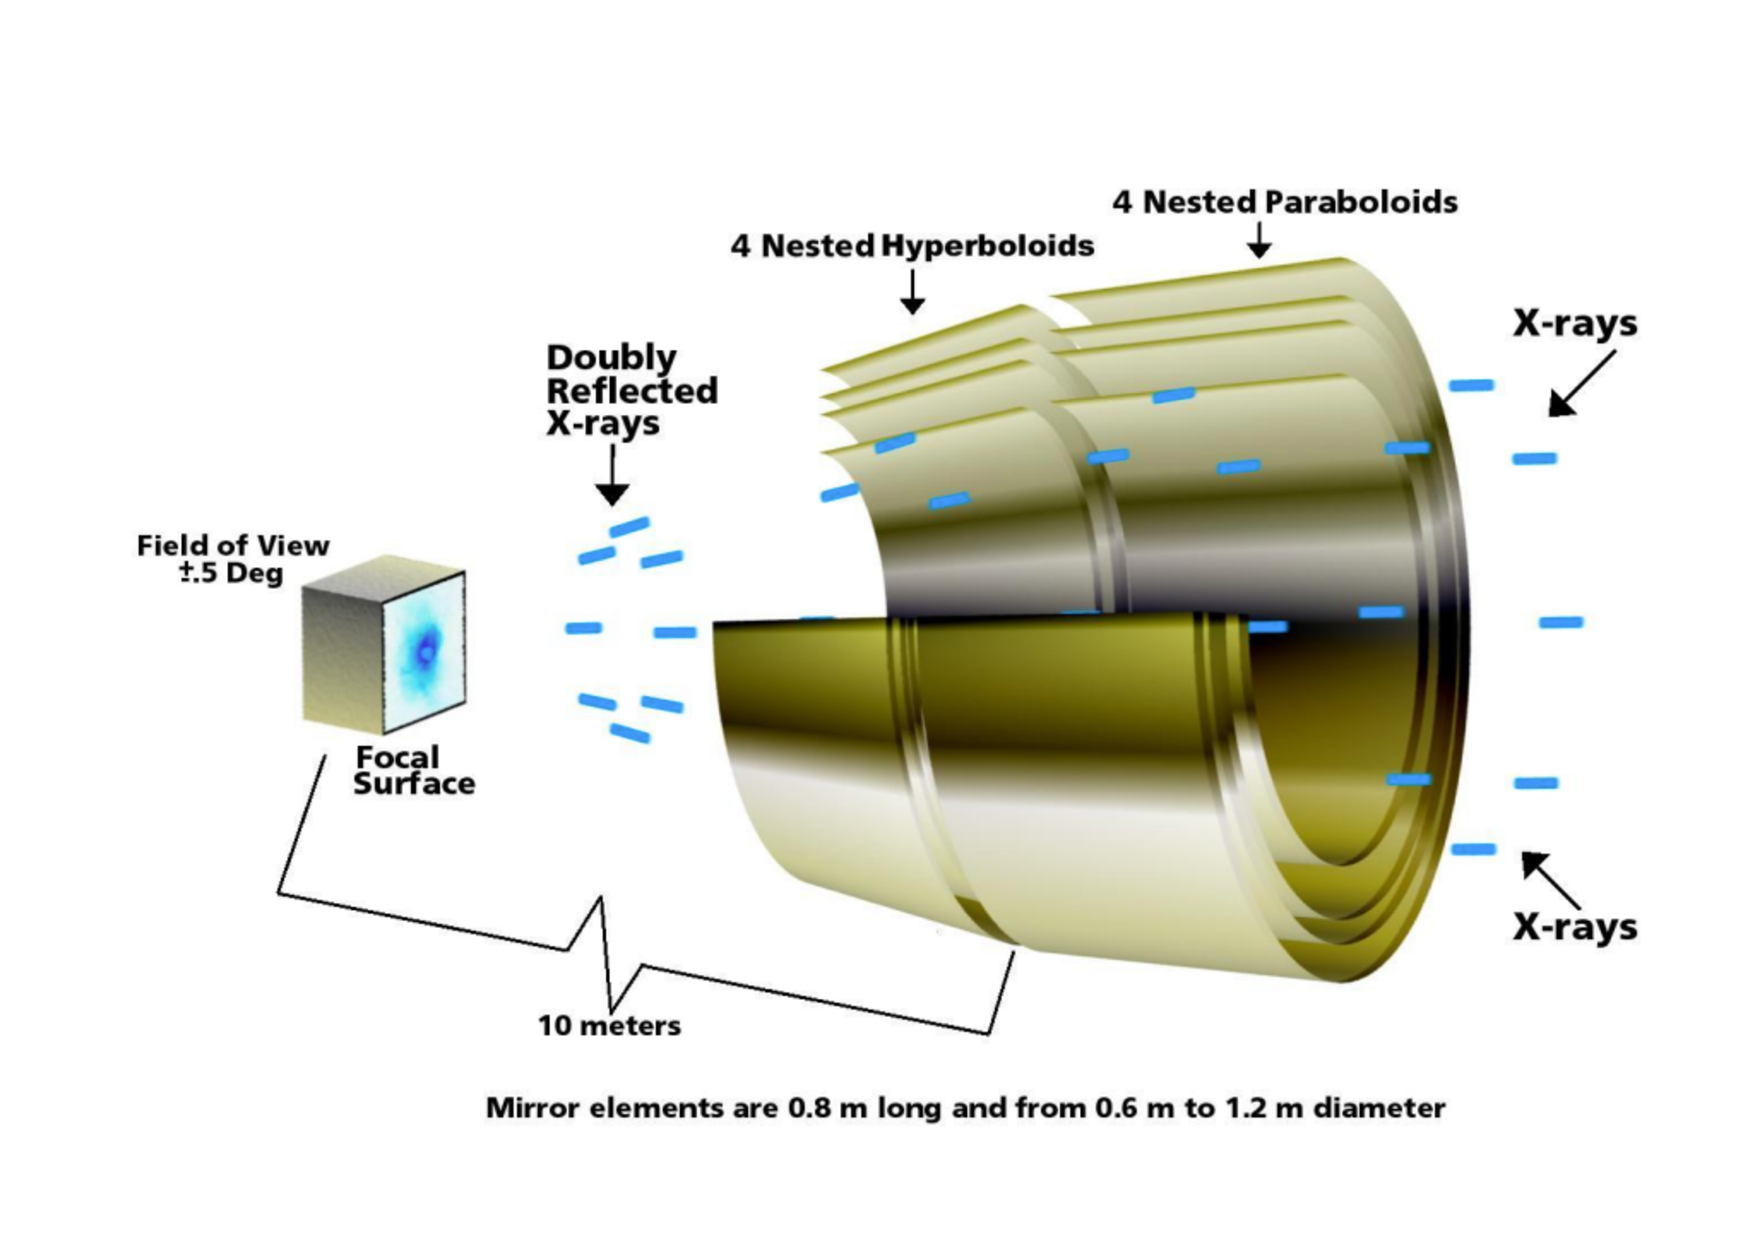
\includegraphics[scale=0.45]{Figures/3-Xray_age/chandra_scheme.pdf}
    \caption{Schematic of \Chandra X-ray telescope. Four nested co-axial, confocal, grazing incident mirrors focus the X-ray photons to a common focal point where the detectors are located. Image Credit: NASA/CXC/ D. Berry}
    \label{fig:diagram_xray_telescope}
\end{figure}

The \XMM X-ray telescope \citep{Jansen_etal_2001} contains three x-ray CCD cameras collectively known as EPIC. EPIC is made up of one PN detector and two metal oxide detectors (MOS 1 and MOS 2). The MOS detectors are located behind the telescopes grating and only receives approximately half of the incident flux. Whereas the PN detector has an unobstructed beam and a much higher signal to noise than the MOS detectors, therefore data analysis is preferably performed with PN observations. The EPIC instrument is capable of imaging over the telescope's 30 arcmin field of view in the energy range 0.2 - 15 keV (62 - 0.826 \AA). Note that due to the short wavelengths of X-ray radiation, wavelengths are preferably presented in terms of energy. All EPIC CCD's operate in a photon counting mode which produces an event list including the position of photon, arrival time and the photon energy; this allows for both imaging and spectra of X-ray objects.

The \Chandra telescope \citep{Weisskopf_etal_2000} has two focal plane instruments: the advanced CCD imaging spectrometer (ACIS) and the high resolution camera (HRC). The HRC provides only images and no spectral information, therefore in this study observations are restricted to ACIS since it provides spectral information in the energy range 0.2 - 10 keV.

\section{Observations and stellar sample}
\subsection{Sample selection}
\label{Section_sample_selection}
Our target stars with well-determined ages were selected from several different sources. The majority stems from asteroseismology where stars were chosen with precisely determined stellar parameters, including ages, from modelling of individual oscillation frequencies as observed by the Kepler satellite \citep{Silva_Aguirre_etal_2015,Silva_Aguirre_etal_2017}. However, for some stars the signal to noise was not high enough to model the individual oscillation frequencies. In these circumstances, the global asteroseismic parameters \citep{Chaplin_etal_2014} are combined with spectroscopic parameters ($T_{eff}$ and [Fe/H]) and ages are obtained through \texttt{BASTA} \citep{Silva_Aguirre_etal_2015}. \texttt{BASTA} uses a Bayesian approach to determine the probability that a set of parameters matches the observed asteroseismic parameters. Nearby stars were selected for dedicated X-ray observations with \XMM and \Chandra (PI: Poppenhaeger).
%Maybe add more in here

The second source is a sample of G and K type stars that are located in wide binaries with a white dwarf companion. As discussed in Section \ref{Section:intro_ages}, the ages of white dwarfs are relatively well known and can act as a stellar chronometer for the binary system. The binaries considered in this study are specifically wide binaries, this is to ensure that any binary companion has not gravitationally interacted with the main sequence star and altered its rotational (and thus magnetic activity) evolution. The sources for these systems are \citet{Garces_etal_2011} and \citet{Zhao_etal_2012}.

While ages have been derived for these systems by \citet{Garces_etal_2011}, more recent work into 3D models of white dwarfs showed that previous fits to 1D models overestimated the effective temperature and surface gravity \citep{Tremblay_etal_2013}. Therefore, a correction was applied to the values calculated in \citet{Garces_etal_2011} by using Equations 7 and 8 from \citet{Tremblay_etal_2013}. With values for the effective temperature and surface gravity, the mass and cooling age of the white dwarfs were calculated using Montreal model grids for white dwarfs with hydrogen atmospheres\footnote{Available at \url{http://www.astro.umontreal.ca/~bergeron/CoolingModels/}} \citep{Holberg_Bergeron_2006,Kowalski_Saumon_2006,Bergeron_etal_2011,Tremblay_etal_2011}. However, to obtain the total age of the white dwarf, the initial-final mass relationship (Equation \ref{Eq:WD_init_final_relationship}) from \citet{Kalirai_etal_2008} was used which allows the mass of the progenitor star to be obtained. Padova stellar evolutionary models \citep{Bertelli_etal_2008} are then used to estimate the main sequence lifetime of the progenitor star which is added to the cooling age of the white dwarf to obtain the total age.

\begin{equation}
    M_{final} = 0.109M_{initial} + 0.394M_{\odot}
    \label{Eq:WD_init_final_relationship}
\end{equation}

The third source includes individually selected stars with archival X-ray observations and relatively well known ages through various methods. these age methods includes asteroseismology (16 Cyg A and B, $\alpha$ Cen / Promixa Cen system), isochrone fitting (61 Cyg A and B) and association with a subpopulation of stars in the galaxy (HR 7703). The Sun is also included in our sample and its age is taken to be $4.57 \pm 0.02$ Gyr \citep{Bahcall_etal_1995}. For the full details on the sample of stars used in this study and the various age methods used see Appendix REF. One may wonder why Proxima Cen is included in our analysis as it is a fully convective star and previous discussion on the age-activity-rotation relationship was focused on stars with a stellar like dynamo (i.e. stars that have radiative core surrounded by a convective envelope). However, recent work by \citet{Wright_Drake_2016} considered a sample of fully convective stars and found that they follow an activity-rotation relationship that is indistinguishable to that of solar-type stars. Since the activity-rotation relationship is a well established proxy for the behaviour of the solar-like dynamo, this results suggest that these fully convective stars exhibit a solar-like dynamo and therefore it was included in the sample.

\subsection{Distances and spectral types}
It is known that the rotational evolution and thus the X-ray luminosity of stars no longer on the main sequence differ than those still on it, therefore only main sequence stars shoud be included in the sample. For several stars from the asteroseismic part of the sample, no luminosity classes were found in the literature. Therefore for these stars, their surface gravity (as calculated from asteroseismology) was compared to the relation of $B-V$ colour and surface gravity as given by \citet{Gray_2005} and shown in Equation \ref{Eq:Gray_2005}. Stars with surface gravities that differed by more than 0.2 dex of the value calculated by Equation \ref{Eq:Gray_2005} were excluded from the sample.

\begin{equation}
    \begin{aligned}
    \log(g) & = 4.25 - 0.3124(B-V) - 0.5022(B-V)^{2} + 6.532(B-V)^{3} \\
    &- 9.9431(B-V)^{4} + 5.7581(B-V)^{5} - 1.1706(B-V)^{6}
    \label{Eq:Gray_2005}
    \end{aligned}
\end{equation}

In order to determine the X-ray luminosity of a star, the distance is required. For the majority of the sample, distances were determined through parallaxes sourced from either SIMBAD \citep{Wenger_etal_2000} or \textit{Gaia} DR1 \citep{Gaia_Collaboration_2016_DR1}. For one star in the asteroseismic part of the sample, no distance or parallax was found in the literature. Therefore, for this star, the Barnes-Evans method was used to calculate the distance. The Barnes-Evans method uses a relation between angular diameter and V-K colour \citep{Fouque_Gieren_1997} shown in Equation \ref{Eq:Fouque_BE_relation} to calculate the angular diameter of a star ($\Theta$ - angular diameter in milli-arcseconds). Since the radius of the star is known through asteroseismology, this can be used with the angular diameter to determine the distance as shown in Equation \ref{Eq:distance_from_angular_diameter} which is derived from trigonometry where $\theta$ is the angular diameter in radians. Since the stars considered in this sample are all located relatively nearby then reddening was not taken into account. The Barnes-Evans method has been used previously to determine the stellar radii of exoplanet host stars and found good agreement with published values \citep{Watson_etal_2010}.

\begin{equation}
    \log\Theta = 0.5474 - 0.2V + 0.262(V-K)
    \label{Eq:Fouque_BE_relation}
\end{equation}

\begin{equation}
    d = \frac{2R_{*}}{\theta}
    \label{Eq:distance_from_angular_diameter}
\end{equation}

Finally, it was necessary to determine the spectral type of the candidates since this influences both the stellar activity and its evolution with time. The stellar spectral types were collected from the SIMBAD \citep{Wenger_etal_2000} database, or estimated from the stellar effective temperatures as published in \citet{Chaplin_etal_2014} and \citet{Silva_Aguirre_etal_2015}.

\section{Data analysis}
This section details the methods used to determine the X-ray luminosity for the sample of stars considered in this work.

Archival data for \XMM were obtained from the XMM-Newton Science Archive and analysed using \texttt{SAS} (Science Analysis system) version $15.0$. The data was filtered to remove any bad pixels or bad events by setting criteria to limit the probability of double photon impact events. This type of event occurs when two photons hit the same or neighbouring pixels in the same readout time frame and causes a slightly different pattern compared to a single photon event. For observations with \XMM, a standard source extraction radius of 20 arcsec is used and a source free background region was chosen with extraction radius of 70 arcsec. Data analysis was also preferably performed with PN observations due to the higher signal to noise from this instrument.

Archival observation files for \Chandra were obtained through the Chandra X-ray Centre public archive and analysed with \texttt{CIAO} (Chandra Interactive Analysis of Observations; \citealt{Fruscione_etal_2006}). For \Chandra data, a standard source extraction radius of 1.5 arcsec was used and a source free background region was chosen with radius of 15 arcsec. For a full list of X-ray observations see Table \ref{table:xray_obs_details}.

\begin{table}[t]
	\resizebox{\textwidth}{!}{
	\centering
	\begin{tabular}{lllc}
		\hline \hline
		Name of Star / White Dwarf & Telescope / Instrument     & Observation ID & Exposure Time / $10^{3}$ s \\
		\hline
		16 Cyg A & \Chandra ACIS-I  & 16647 & 35.33 \\
		 & \Chandra ACIS-I   & 18756 & 38.57 \\
		16 Cyg B & \Chandra ACIS-I  & 16647 & 35.33 \\
		 & \Chandra ACIS-I  & 18756 & 38.57 \\
		40 Eri A/40 Eri B & \Chandra ACIS-S  & 13644  & 5.00 \\
		61 Cyg A & \textit{XMM} PN Thick Filter & 41740301$^*$ & 7.09  \\
		61 Cyg B  & \textit{XMM} PN Thick Filter & 41740301$^*$  & 7.09 \\
		CD -3710500 / L481-60 & \Chandra ACIS-I   & 13769 & 24.75 \\
		GJ 176 & \Chandra ACIS-S  & 13638 & 4.98  \\
		GJ 191 & \Chandra ACIS-S   & 13646 & 5.00 \\
		HR 7703 & \textit{XMM} PN Thick Filter & 670380401 & 7.95  \\
		KIC 10016239 & \textit{XMM} PN Medium Filter & 761560601 & 22.24  \\
		KIC 12011630 & \Chandra ACIS-I HETG  & 9969 & 19.74 \\
		KIC 3123191 & \Chandra ACIS-I  & 13166 & 2.72 \\
		KIC 5309966 & \Chandra ACIS-I   & 17138 & 26.43 \\
		 & \Chandra ACIS-I  & 17141 & 29.69  \\
		 & \Chandra ACIS-I  & 17513 & 49.40 \\
		 & \Chandra ACIS-I  & 17516  & 49.02  \\
		KIC 6116048 & \textit{XMM} PN Medium Filter & 722330201 & 11.58 \\
		 & \textit{XMM} PN Medium Filter & 722330301 & 10.73 \\
		KIC 6603624 & \textit{XMM} PN Medium Filter & 761560701 & 35.67 \\
		KIC 7529180  & \textit{XMM} PN Thin Filter & 743460201 & 18.07 \\
		KIC 8292840 & \textit{XMM} PN Medium Filter & 743840201 & 10.74 \\
		KIC 9025370 & \textit{XMM} PN Medium Filter & 761560501 & 8.92 \\
		KIC 9410862 & \textit{XMM} PN Medium Filter & 670140501 & 26.36\\
		KIC 9955598 & \textit{XMM} PN Medium Filter & 761560601 & 22.24 \\
		NLTT 7887 / NLTT 7890 & \textit{XMM} PN Medium Filter & 670650101 & 16.60  \\
		Proxima Centauri & \textit{XMM} PN Medium Filter & 551120201$^*$ & 26.49 \\
		Alpha Centauri B & \textit{XMM} PN Thick Filter & 760290301$^*$ & 14.88 \\     
		\hline
		\end{tabular}}
		\caption[List of X-ray observations used in study]{Table of observations that were fully analysed and presented in the results Section. $^*$A large number of observations exist for these targets and has been taken into account in our analysis; one specific observation is listed to illustrative typical exposure times.}
		\label{table:xray_obs_details}
\end{table}

\subsection{Source detection}
For each target, the data was tested to see if a source was significantly detected in X-rays using the images from the observations. The number of X-ray counts were extracted from the source and background region from 0.2 - 2.0 keV as this is the region where weakly active cool stars emit most of their X-ray emission.

For \XMM data, there is typically a significant background signal detected in any observation. Therefore, the number of counts expected from a pure background  ($C_{0}$) was estimated by scaling the number of counts detected in the background region to the number expected in an area equivalent to the source region as shown in Equation \ref{Eq:C0_equation} where $C_{b}$ is the number of counts in the background region and $R_{b}$ and $R_{s}$ are the radii of the background and source regions, respectively. The number of counts in the source region ($C_{s}$) is then compared to the $C_{0}$ value and if it exceeds this value by $3\sigma$ then an X-ray source has been detected, otherwise an upper limit is calculated using the $3\sigma$ level over the background signal. Note that $\sigma$ is estimated to be the square root of the number of expected background counts ($C_{0}$). 

\begin{equation}
    C_{0} = \frac{C_{b}}{R_{b}^{2}}R_{s}^{2}
    \label{Eq:C0_equation}
\end{equation}

For \Chandra data, the background signal is typically very low meaning that estimating $\sigma$ as the square root of $C_{0}$ is invalid. Therefore, full Poisson statistics were used and the inverse per cent point function was calculated at which, for a given expected number of background counts (i.e. $C_{0}$), the number of counts in the source region had a probability of less than 0.3 per cent of occurring as a random fluctuation. If the number of source counts was greater than this value then the source was detected; otherwise, that number was used as the upper limit on the X-ray counts for the source. For both \Chandra and \XMM data, the fractional error on $C_{s}$ was taken to be $\frac{\sqrt{C_{s}}}{C_{s}}$.

\subsection{Stellar variability}
The typical exposure time for an X-ray observation is on the order of 10 ks ($\approx$ few hours), however, stars can have variability that occurs on shorter time-scales than this. Therefore, for detected target stars, a light curve was extracted from each observation to check for short-term magnetic phenomena such as flares. This is important as flares release a large amount of energy which causes the corona to heat up thus increasing the temperature and emission measure of the corona (emission measure simply means the amount of material that emits at a particular temperature and is used in spectral fitting - see Section \ref{Section_Determining_Xray_flux}). If flares are detected in our observations, it can result in a significantly higher X-ray luminosity than the quiescent emission level of the star.

\begin{figure}
    \centering
    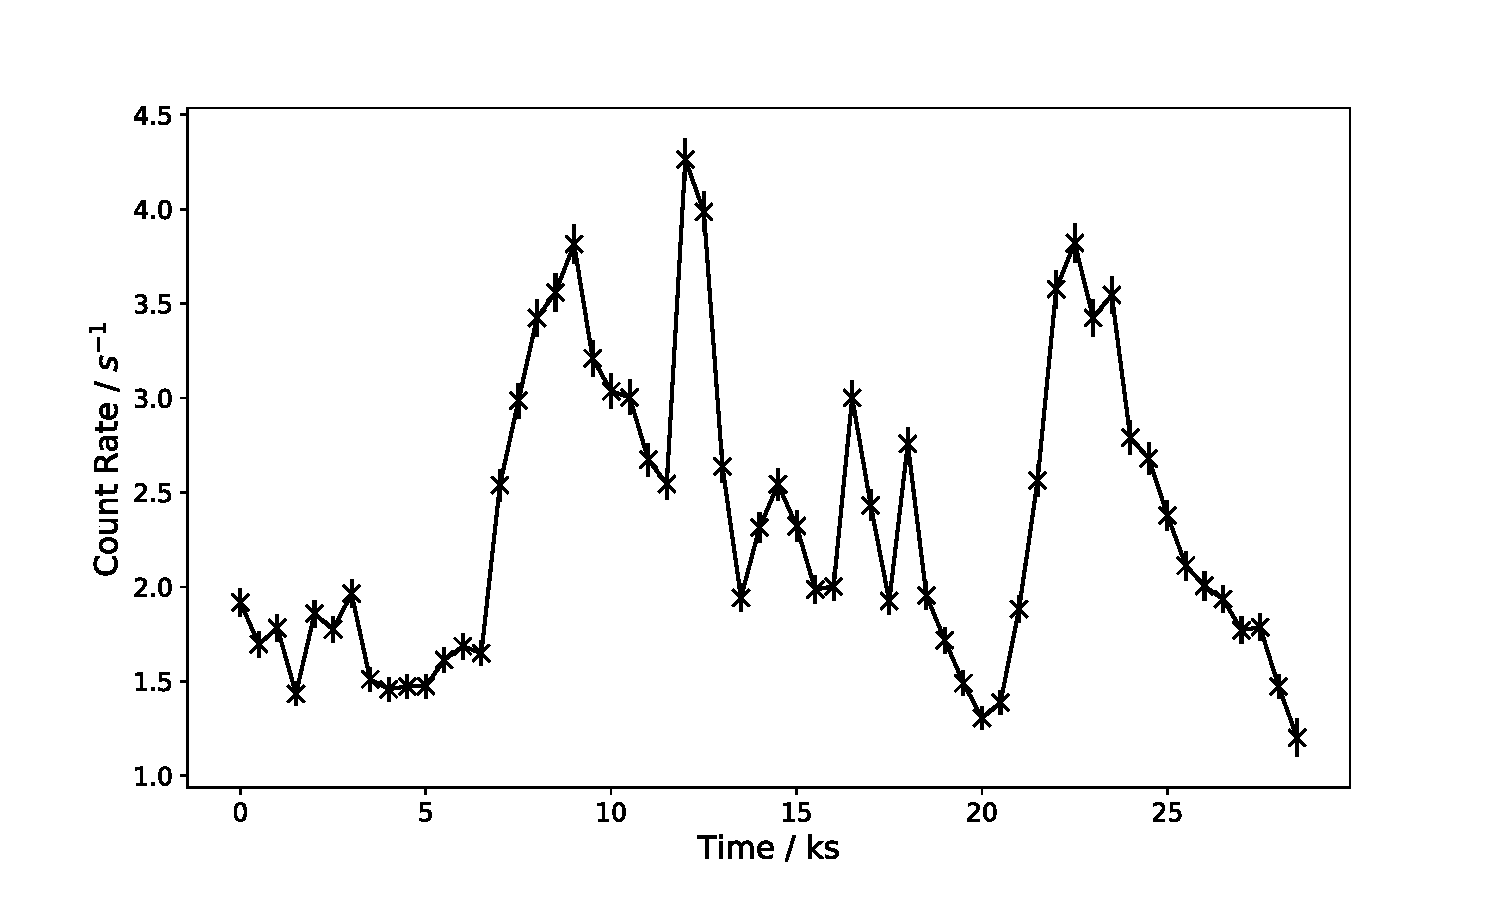
\includegraphics[scale=0.5]{Figures/3-Xray_age/proxima_cen_lc.pdf}
    \caption[X-ray light curve of Proxima Centauri]{X-ray light curve of Proxima Centauri. This plot shows the count rate during the observation and would suggest that several flares occurred during this time.}
    \label{fig:proxima_cen_lc}
\end{figure}

\begin{figure}
    \centering
    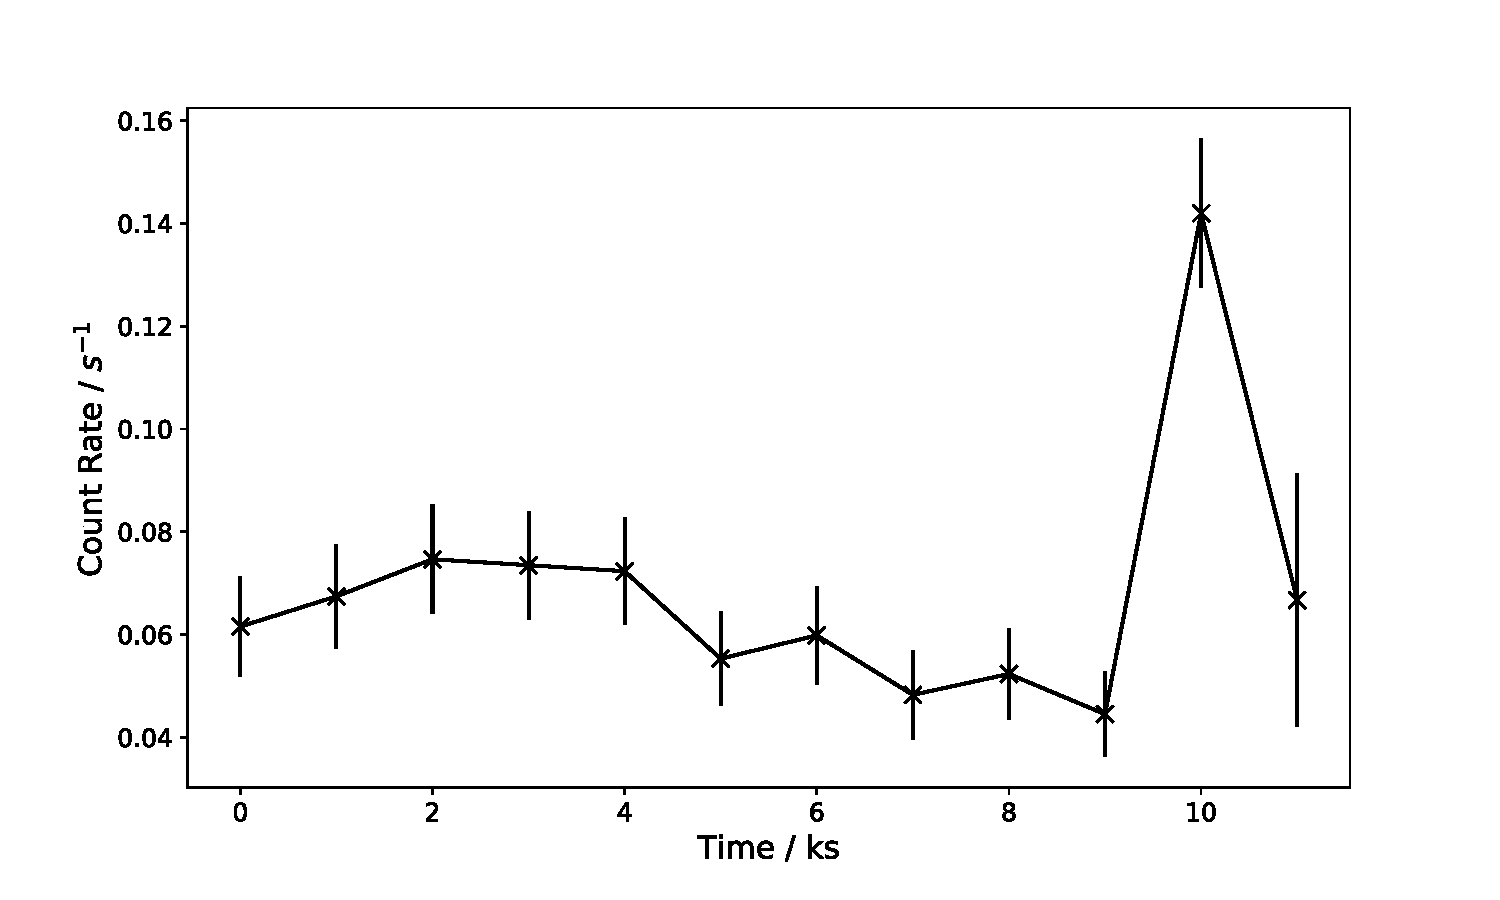
\includegraphics[scale=0.5]{Figures/3-Xray_age/HR7703_lc.pdf}
    \caption[X-ray light curve of HR 7703]{X-ray light curve of HR 7703. This plot shows the count rate during the observation and would suggest that a flare occurred towards the end of this observation.}
    \label{fig:HR7703_lc}
\end{figure}

In the case of Proxima Centauri, the light curve showed several rapid increases in the count rate over the observation exposure time, indicating several flares as shown in Figure \ref{fig:proxima_cen_lc}. Therefore, the quiescent value for the X-ray luminosity of $4.9 \times 10^{26}$ erg $s^{-1}$ was taken from \citet{Fuhrmeister_etal_2011} and used in this work. An inspection of the light curve for HR 7703 indicated that a flare had occurred towards the end of the observation as shown in Figure \ref{fig:HR7703_lc}. In this case, the time interval associated with the flare was excluded from the data analysis.

\subsection{Determining the X-ray flux}
\label{Section_Determining_Xray_flux}
For X-ray sources with significant detections and where the source region contained $\approx 90$ or more counts, the spectra of the source was modelled with a coronal plasma model in order to determine the X-ray flux. A spectrum for the star was extracted from the observations using the relevant analysis tools for each telescope. The extracted spectra were fitted with an optically thin thermal plasma model (APEC model) using the \texttt{XSPEC} fitting software. The APEC model has four parameters: coronal temperature (keV), metal abundances, redshift and emission measure. The emission measure is simply a measure of the amount of material that is emitting at a certain temperature and is defined by Equation REF \textcolor{red}{INSERT EQ AND DEF OF EMISSION MEASURE}. Since all of the stars considered in this sample are located nearby then the redshift was fixed at zero; the abundances were assumed to be solar by using abundances from \citet{Grevesse_Sauval_1998}. Using solar abundances is a reasonable approximation for fairly low-resolution spectra as no significant spectral features are resolved that are highly dependent on metallicity abundances. \textcolor{red}{Check the reason with Katja}
Therefore, the two parameters that were fitted are coronal temperature and emission measure; in some cases, two temperature components were required to find a suitable fit for the coronal spectrum. The \texttt{XSPEC} fitting software uses a modified Levenberg-Marquardt algorithm to minimise the fit statistic and is based on \texttt{CURFIT} from \citet{Bevington_1969}. However, the Levenberg-Marquardt algorithm only finds the local minimum which is not necessary the global minimum, therefore, the initial conditions for each parameter that is to be fitted must be reasonable. From the best-fitting model to each object, the flux was then calculated in a fixed energy band from 0.2 to 2 keV. The details and plots of the best-fitting models are shown in Table \ref{table:spectral_fit_details} and Appendix \ref{Appendix_Xray_spectra}, respectively

\begin{table}[h]
\centering
\caption[X-ray spectral modelling results]{Best-fitting model parameters used to calculate the X-ray flux between 0.2 and 2.0 keV for stars that were sufficiently detected in X-rays.}
\begin{tabular}{l c c c}
	\hline \hline
	Name of Star & Model kT & Model Emission Measure  & Reduced chi-squared\\
    & (keV)          &($\frac{4\pi d^2}{10^{-14}}$ cm$^{-3}$) & \\
	\hline
	40 Eri A & 0.19 & $9.9\times 10^{-5}$ & 1.59\\
	CD -3710500 & 0.44 & $2.2\times 10^{-4}$ & 0.32\\
	GJ 176 & 0.37 & $3.4\times 10^{-5}$ & 1.49\\
	GJ 191 & 0.30 & $5.4\times 10^{-5}$ & 2.52\\
	HR 7703 & 0.17 & $5.31\times 10^{-5}$ & 1.34\\
	& 0.76 & $1.45\times 10^{-5}$  &\\
	KIC 7529180 & 0.22 & $9.8\times 10^{-6}$ & 1.70\\
	& 0.91 & $1.7\times 10^{-5}$  &\\
	61 Cyg A & 0.21 & $4.09\times 10^{-4}$ & 1.99\\
	& 0.79 & $1.75\times 10^{-4}$  &\\
	61 Cyg B & 0.19 & $1.71\times 10^{-4}$ & 1.17\\
	& 0.67 & $5.06\times 10^{-4}$  &\\
	\hline
	\end{tabular}
	\label{table:spectral_fit_details}
\end{table}

In the case where the source region contained $\approx$ 90 counts or less, then typically there were not enough data points to fit a spectrum accurately. Therefore, an estimate of the X-ray flux was obtained through WebPIMMS\footnote{\url{https://heasarc.gsfc.nasa.gov/cgi-bin/Tools/w3pimms/w3pimms.pl}} using the mean count rate of the source region. A typical spectrum was assumed for the stellar corona, and WebPIMMS calculated the source flux using the instrument characteristics. The X-ray flux was calculated in the $0.2 - 2.0$ keV energy range assuming an APEC model of solar abundance and $\log T$ value of 6.5 ($T \approx 3$ MK), appropriate for inactive cool stars. The conversion factors from counts to flux used for each of the instruments are shown in Table \ref{table:webpimms_conversion_factors}; note that the sensitivity of \Chandra changes significantly over the years of operation, and therefore the correct conversion factors need to be chosen for the observing cycle in which a given observation took place. For \XMM observations, the encircled energy fraction factor needs to be applied as well since its point spread function (PSF) is significantly larger than typical practical source extraction radii. Since a 20 arcsec source radius, this encloses approximately 80\% of the PSF and thus any count rates observed were corrected by dividing by $0.8$.

\begin{table}
	\caption{Conversion factors used by WebPIMMS to convert number of counts into flux in the $0.2 - 2.0$ keV energy range, assuming a coronal temperature of $\log T = 6.5$ and solar abundances.}
	\centering
	\begin{tabular}{l c}
		\hline \hline
		Name of Instrument & Conversion Factor \\
         & (erg s$^{-1}$ cm$^{-2}$ count$^{-1}$) \\ 
		\hline
		XMM PN Medium Filter & $1.03\times10^{-12}$\\
		Chandra ACIS-I No Grating (Cycle 16) & $2.42\times10^{-11}$\\
		Chandra ACIS-I No Grating (Cycle 12) & $1.52\times10^{-11}$\\
		Chandra ACIS-I HET Grating (Cycle 10) & $2.16\times10^{-10}$\\
		\hline
	\end{tabular}
	\label{table:webpimms_conversion_factors}
\end{table}

The statistical error on the values of X-ray counts was calculated from the square root of the number of source counts ($C_{s}$) (as the distribution is described by Poisson statistics) and divided by the number of source counts to obtain a fractional error. This fractional error on the number of counts was also used as the error on the X-ray flux and the X-ray luminosity. However, the X-ray luminosity of a star is known to vary on various time-scales, including time-scales much shorter than the star’s main-sequence lifetime, therefore a minimum physical error of 0.1 dex in $\log L_{x}$ was applied to the data to account for this variability, even if the statistical error was smaller. This value was determined from the long-term X-ray monitoring of 61 Cyg B \citep{Robrade_etal_2012}, a star without an apparent activity cycle, where the standard deviation of the X-ray luminosity was at 0.1 dex over several years of observations. In order to convert X-ray flux into X-ray luminosity, Equation \ref{Eq:flux_luminosity} was used.

\begin{equation}
    L_{x} = 4\pi d^{2}F_{x}
    \label{Eq:flux_luminosity}
\end{equation}

\subsection{Additional notes on analysis}
In the previous section, the general methodology used to determine the X-ray luminosity is detailed. However, since the sample is made up of a number of observations from both the \XMM and \Chandra telescopes, additional details are presented here about the individual observations used and the data reduction.

\textit{16 Cyg A}: This star was detected by combining two \Chandra observations on a front-illuminated CCD, which only provides energy sensitivity above 0.6 keV. The flux was extrapolated for the full $0.2 - 2.0$ keV band by using WebPIMMS and assuming a coronal temperature of $\log T = 6.5$. The star 16 Cyg B was covered by the same observations, but is undetected and an upper limit is calculated. There is also an earlier, shorter \XMM observation covering both stars, but they were npth undetected in that observation, which is consistent with the \Chandra data.

\textit{40 Eri A}: This star is in a wide binary system with the white dwarf 40 Eri B, with a projected distance of 83 arcsec \citep{Wenger_etal_2000}, translating to a physical distance of ca. 400 AU. Using the techniques outlined in Section \ref{Section_sample_selection}, its reported $T_{eff}$ and $\log g$ values \citep{Zhao_etal_2012} to calculate an age of $3.70^{+3.57}_{-1.34}$ Gyr for 40 Eri B, which is adopted as the age of the system. 40 Eri A was observed with a back-illuminated \Chandra CCd, which provides energy sensitivity above 0.245 keV. A spectral fit was performed and the X-ray flux was extrapolated for the full $0.2 - 2.0$ keV energy range. There is also a third star, 40 Eri C, present in the system; however, it is close enough to the white dwarf (ca 35 AU) that its rotation and activity properties may have been affected during the evolution of the white dwarf progenitor, which is why 40 Eri C is not included in the analysis.

\textit{61 Cyg A and B}: these stars have been monitored in X-rays with \XMM over several years. On exemplary X-ray spectrum for each star is shown in Figure \ref{App_A_61Cyg}. 61 Cyg A has been found to display an activity cycle \citep{Robrade_etal_2012}, and the full range of observed X-ray luminosities have been adopted as the error bar for 61 Cyg A's X-ray luminosity found in this work. 61 Cyg B has found to have a flat activity profile \citep{Robrade_etal_2012}, and the mean X-ray luminosity is adopted in this analysis with the standard deviation over all X-ray observations as the error on this value.

\textit{CD-3710500}: This star is in a wide binary system with the white dwarf L481-60. Using the techniques outlined in Section \ref{Section_sample_selection}, its reported $T_{eff}$ and $\log g$ values \citep{Zhao_etal_2012} to calculate an age of $1.77^{+0.65}_{-0.27}$ Gyr for L481-60, which is adopted as the age for the system. The star CD-3710500 was observed with a front-illuminated \Chandra CCD, which provides energy sensitivity above 0.6 keV. A spectral fit was performed and the X-ray flux was extrapolated for the full $0.2 - 2.0$ keV energy range.

\textit{GJ 176}: This star was detected with a back-illuminated \Chandra CCD, which provides energy sensitivity above 0.245 keV. A spectral fit was performed and the X-ray flux was extrapolated for the full $0.2 - 2.0$ keV energy range.

\textit{GJ 191}: This star was detected with a back-illuminated \Chandra CCD, which provides energy sensitivity above 0.245 keV. A spectral fit was performed and the X-ray flux was extrapolated for the full $0.2 - 2.0$ keV energy range. The X-ray luminosity found is consistent with the values reported by \citet{Guinan_etal_2016}.

\textit{HR 7703}: This source was detected with \XMM and a spectral fit was performed for the full energy range of $0.2 - 2.0$ keV.

\textit{KIC 12011630, KIC 3123191 and KIC 5309966}: These stars were in the field of view of \Chandra during observations of other targets and are all undetected in X-rays. The sources are located on front-illuminated CCD's and are far from the centre of the field of view. Since \Chandra's PSF becomes large at the edges of the field of view, large extraction regions had to be used, which led to quite high upper limits for the X-ray luminosities for these stars.

\textit{KIC 10016239 and KIC 7529180}: These stars were detected with \XMM. KIC 7529180 was detected with a sufficient number of source counts so that a spectral fit could be performed. For KIC 10016239, the excess source counts were used to calculate the X-ray flux through WebPIMMS, assuming a coronal temperature of $\log T = 6.5$.

\textit{KIC 6116048, KIC 6603624, KIC 8292840, KIC 9025370, KIC 9410862}: These stars were observed with \XMM, but undetected in X-rays.

\textit{KIC 9955598}: This star was observed and detected with \XMM. Since there is another X-ray source at close projected distance (ca.\ $20$ arcsec), we chose an extraction region with a radius of $10$ arcsec instead of $20$ arcsec, and applied the correct encircled energy fraction factor (0.6) to account for the smaller extraction region when calculating the flux.

\textit{NLTT 7887}: This star is in a wide binary system with the white dwarf NLTT 7890. Since the reported surface gravity of the white dwarf has large errors \citep{Garces_etal_2011}, the age we derive has large errors as well with $4.97^{+8.8}_{-3.0}$~Gyr. The star NLTT 7887 was covered by an \XMM observation, but is undetected.

\textit{$\alpha$ Cen A, $\alpha$ Cen B, Proxima Cen}: The age of this triple system has been derived from asteroseismic observations of $\alpha$ Cen A and $\alpha$ Cen B using different underlying models \citep{Miglio_Montalban_2005}; the mean of the asteroseismic age estimates has been adopted as the age of the system. $\alpha$ Cen A and $\alpha$ Cen B have been monitored in X-rays with \XMM \citep{Robrade_etal_2012}. $\alpha$ Cen B was found to display an activity cycle, and the full range of observed X-ray luminosities is used as the error bar on its X-ray luminosity for our analysis. $\alpha$ Cen A is reported by the same authors to potentially be in an activity cycle as well, however only the low-activity part has been observed so far, and there is no information on what its X-ray luminosity might be during the high-activity part of the cycle. Therefore $\alpha$ Cen A has not been included in this analysis. Proxima Cen has been observed with \XMM several times as well, including multiple stellar flares; a detailed analysis is given by \citet{Fuhrmeister_etal_2011}. Their quiescent X-ray luminosity of $\log L_{\mathrm{X}} = 26.69$ for Proxima Cen has been adopted in this analysis due to the number of flares seen in the observation (see Figure \ref{fig:proxima_cen_lc}).

\section{Results}
\subsection{Magnetic activity across spectral types}
It is known that there is a mass dependence on the rotational spin-down of late-type stars, as many rotational studies include a colour term as a proxy for mass (e.g. \citealt{Barnes_2003,Barnes_2010,Angus_etal_2015}). This is due to the varying depth of the convection zone, F stars have a much thinner convection zone which results in rotational spin-down that occurs on a different timescale than M dwarfs that have a much thicker convection zone \textcolor{red}{(try and expand this point)}. This mass dependence seen in the rotational spin-down will also be present in the evolution of X-ray luminosity with time across varying spectral types. Since the sample of stars considered in this work is relatively small, splitting the sample into different spectral types is non-ideal and an analysis of the whole sample is preferable.

When dealing with X-ray luminosity as a magnetic activity indicator, some studies normalise $L_{x}$ by the stellar bolometric luminosity and then split into different mass bins \citep{Preibisch_Feigelson_2005,Jackson_etal_2012}. However, a different approach was taken by \citet{Schmitt_Liefke_2004}; in their volume complete sample of cool stars in the solar neighbourhood, it was found that when the X-ray luminosity is divided by the stellar surface area $4\pi R_{*}^{2}$ with $R_{*}^{2}$ being the stellar radius, i.e. when one considers the X-ray flux through the stellar surface as a quantity of interest, then stars of all spectral types from F to M show the same spread in this quantity. We visualise these various quantities in Figure \ref{fig:Lx_normalise_schmitt_data}. The stars from \citet{Schmitt_Liefke_2004} were used to plot X-ray luminosity as a function of absolute stellar brightness as a proxy for stellar mass. Preference was given to data collected with the PSPC detector without the Boron filter if several observations were reported in \citet{Schmitt_Liefke_2004}(\textcolor{red}{Explain why}). Using "A Modern Mean Dwarf Stellar Color and Effective Temperature Sequence"\footnote{\url{http://www.pas.rochester.edu/~emamajek/EEM_dwarf_UBVIJHK_colors_Teff.txt}} \citep{Pecaut_Mamajek_2013}, the reported spectral types \citep{Schmitt_Liefke_2004} were used to find estimates for the effective temperature ($T_{eff}$) and bolometric magnitude ($M_{BOL}$). The bolometric magnitude was then used to calculate the bolometric luminosity using Equation \ref{Eq:bolometric_luminosity} where $L_{BOL\odot}$ is the solar bolometric luminosity ($3.827 \times 10^{33}$ \textcolor{red}{check units of this}) and $M_{BOL\odot}$ is the solar bolometric magnitude ($4.7554$). The stellar radius was calculated using Equation \ref{Eq:stellar_radius} where $k$ is the Boltzmann constant and has a value of $5.6704 \times 10^{-5}$ erg cm$^{-2}$ s$^{-1}$ K$^{-4}$. 

\begin{equation}
    L_{BOL} = L_{BOL\odot} 2.5^{M_{BOL\odot} - M_{BOL}}
    \label{Eq:bolometric_luminosity}
\end{equation}

\begin{equation}
    L_{BOL} = 4\pi R_{*}^{2}kT_{eff}^{4}
    \label{Eq:stellar_radius}
\end{equation}

Figure \ref{fig:Lx_normalise_schmitt_data} shows the comparison between X-ray luminosity, X-ray luminosity normalised by stellar surface area and X-ray luminosity normalised by bolometric luminosity. In the left panel of Figure \ref{fig:Lx_normalise_schmitt_data}, the intrinsic mass dependency of X-ray luminosity as a function of mass is clearly seen with higher mass stars typically being more active than lower mass stars. In the right panel of Figure \ref{fig:Lx_normalise_schmitt_data}, the X-ray luminosity normalised by the bolometric luminosity is shown; this shows that lower mass stars typically have higher values on this activity scale, opposite to the trend seen in the X-ray luminosity. This is most likely due to the dependency of bolometric luminosity on both the stellar radius and effective temperature (see Equation \ref{Eq:stellar_radius}), where the extreme differences in effective temperatures from F to M dwarfs cause the trend shown here. Whereas if the X-ray luminosity through the stellar surface area is considered (as shown in the middle panel of Figure \ref{fig:Lx_normalise_schmitt_data}), a flat distribution is seen as a function of absolute magnitude (the proxy for mass in this plot) as reported by \citet{Schmitt_Liefke_2004}.

\begin{figure}
    \centering
    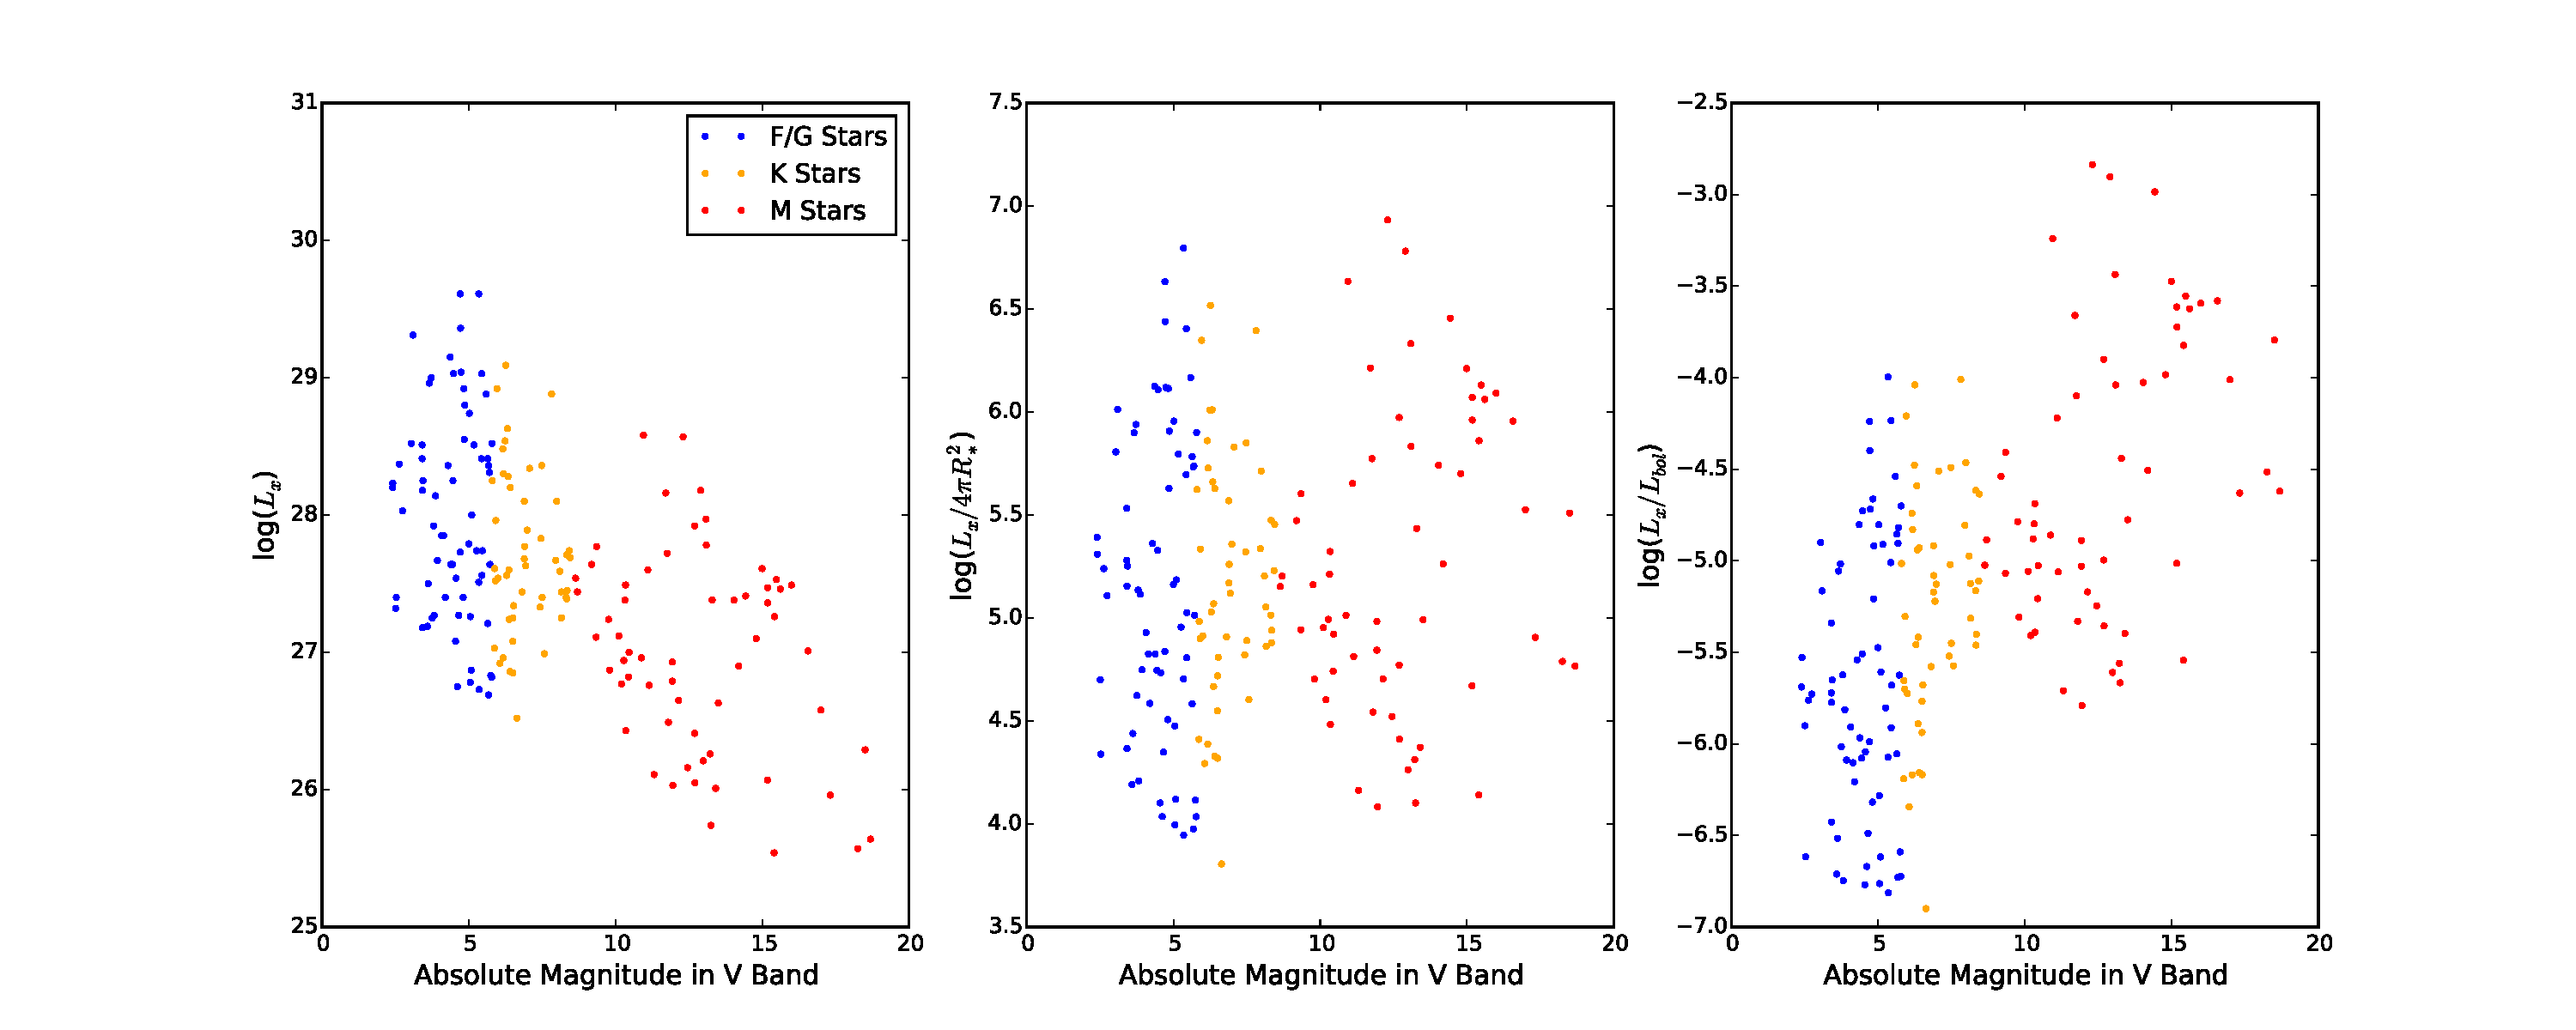
\includegraphics[scale=0.33]{Figures/3-Xray_age/normalise_schmitt_data.pdf}
    \caption[Comparison of X-ray luminosity and normalised parameters]{Comparison of data taken from \citet{Schmitt_Liefke_2004} when normalised by bolometric luminosity and stellar surface. \textbf{Left Panel}: Logarithmic value of X-ray luminosity as a function of absolute magnitude in V band. \textbf{Middle Panel}: Logarithmic value of X-ray luminosity normalised by the stellar surface area as a function of absolute magnitude in V band. \textbf{Right Panel}: Logarithmic value of the ratio of X-ray luminosity to bolometric luminosity as a function of absolute magnitude in V band.}
    \label{fig:Lx_normalise_schmitt_data}
\end{figure}

Therefore, the X-ray luminosities of the sample of cool, inactive stars considered in this work were normalised by the stellar surface area as this allowed for a combined analysis of the full sample to be performed. The stellar radii for the stars in the sample were taken either from asteroseismology or calculated using the same technique described previously for the \citet{Schmitt_Liefke_2004} sample using absolute brightness and effective temperature.



\subsection{Fitting the data}


\section{Discussion}


\section{Conclusions}










\newpage
% Chapter Template

\chapter{Chromospheric emission - age relationship} % Main chapter title

\label{Chapter4} % Change X to a consecutive number; for referencing this chapter elsewhere, use \ref{ChapterX}

\epigraph{\itshape There is a way out of every box, a solution to every puzzle; it's just a matter of finding it.}{---Captain Jean-Luc Picard, \itshape Star Trek}

\section{Introduction}
\textcolor{red}{RB: If this paper is published before submitting - put paragraph similar to the one in Chapter 3 here!}

In \citet{Booth_etal_2017} a steepening of the age-activity relationship was found using X-ray observations coupled to asteroseismic ages. While this study provided the first step to studying the X-ray luminosity-age relationship beyond a gigayear, using the X-ray luminosity as a magnetic activity indicator may not be the most accessible indicator as it requires significant observational resources on an X-ray telescope. An alternative magnetic activity indicator is chromospheric emission in spectral lines such as \caII or H$-\alpha$. Particularly for exoplanet host stars, optical spectra are usually obtained to confirm the presence of candidate exoplanets through radial velocity measurements; therefore making chromospheric emission a much more commonly used magnetic activity indicator.

Chromospheric emission is a widely used activity indicator, particularly for the age-activity relationship and there have been several studies in recent years that use this indicator to calibrate the relationship. However, some debate remains over the suitability of chromospheric emission seen in \caII lines as an age indicator for older stars (i.e. $> 1$ Gyr). \citet{Pace_2013} shows an L-shaped age-activity plot and suggested that the evolution of the chromospheric emission in the \caII lines stopped relatively early. On the contrary, \citet{Lorenzo_Oliveira_etal_2016} showed that when the mass and metallicity of the star is taken into account, chromospheric ages show good agreement with asteroseismic ages. Yet, both of these studies use isochronal ages to calibrate their relationships, asteroseismic ages have not been studied in relation to the chromospheric emission - age relationship. Therefore, the aim of this work was to investigate the age-activity relationship beyond a gigayear using chromospheric emission as a magnetic activity indicator coupled with asteroseismic ages to help shed light on its suitability as an age indicator. An analysis of the \Halpha spectral line was also conducted and is discussed in Section \ref{Chp4_halpha}.

\subsection{Echelle spectrographs}

The observations utilised in this work are high-resolution spectra from two echelle spectrographs: \esp and \narval (see Section \ref{Chp4_obs_spectra}). In a traditional spectrograph, a dispersing element such as a prism or grating is used to split the light into its constituent wavelengths. This results in a single spectrum which is imaged with a CCD; it is the size of the CCD that limits the wavelength range covered. In this traditional spectrograph setup, much of the CCD is not utilised because a single spectrum is produced.

\begin{figure}
    \centering
    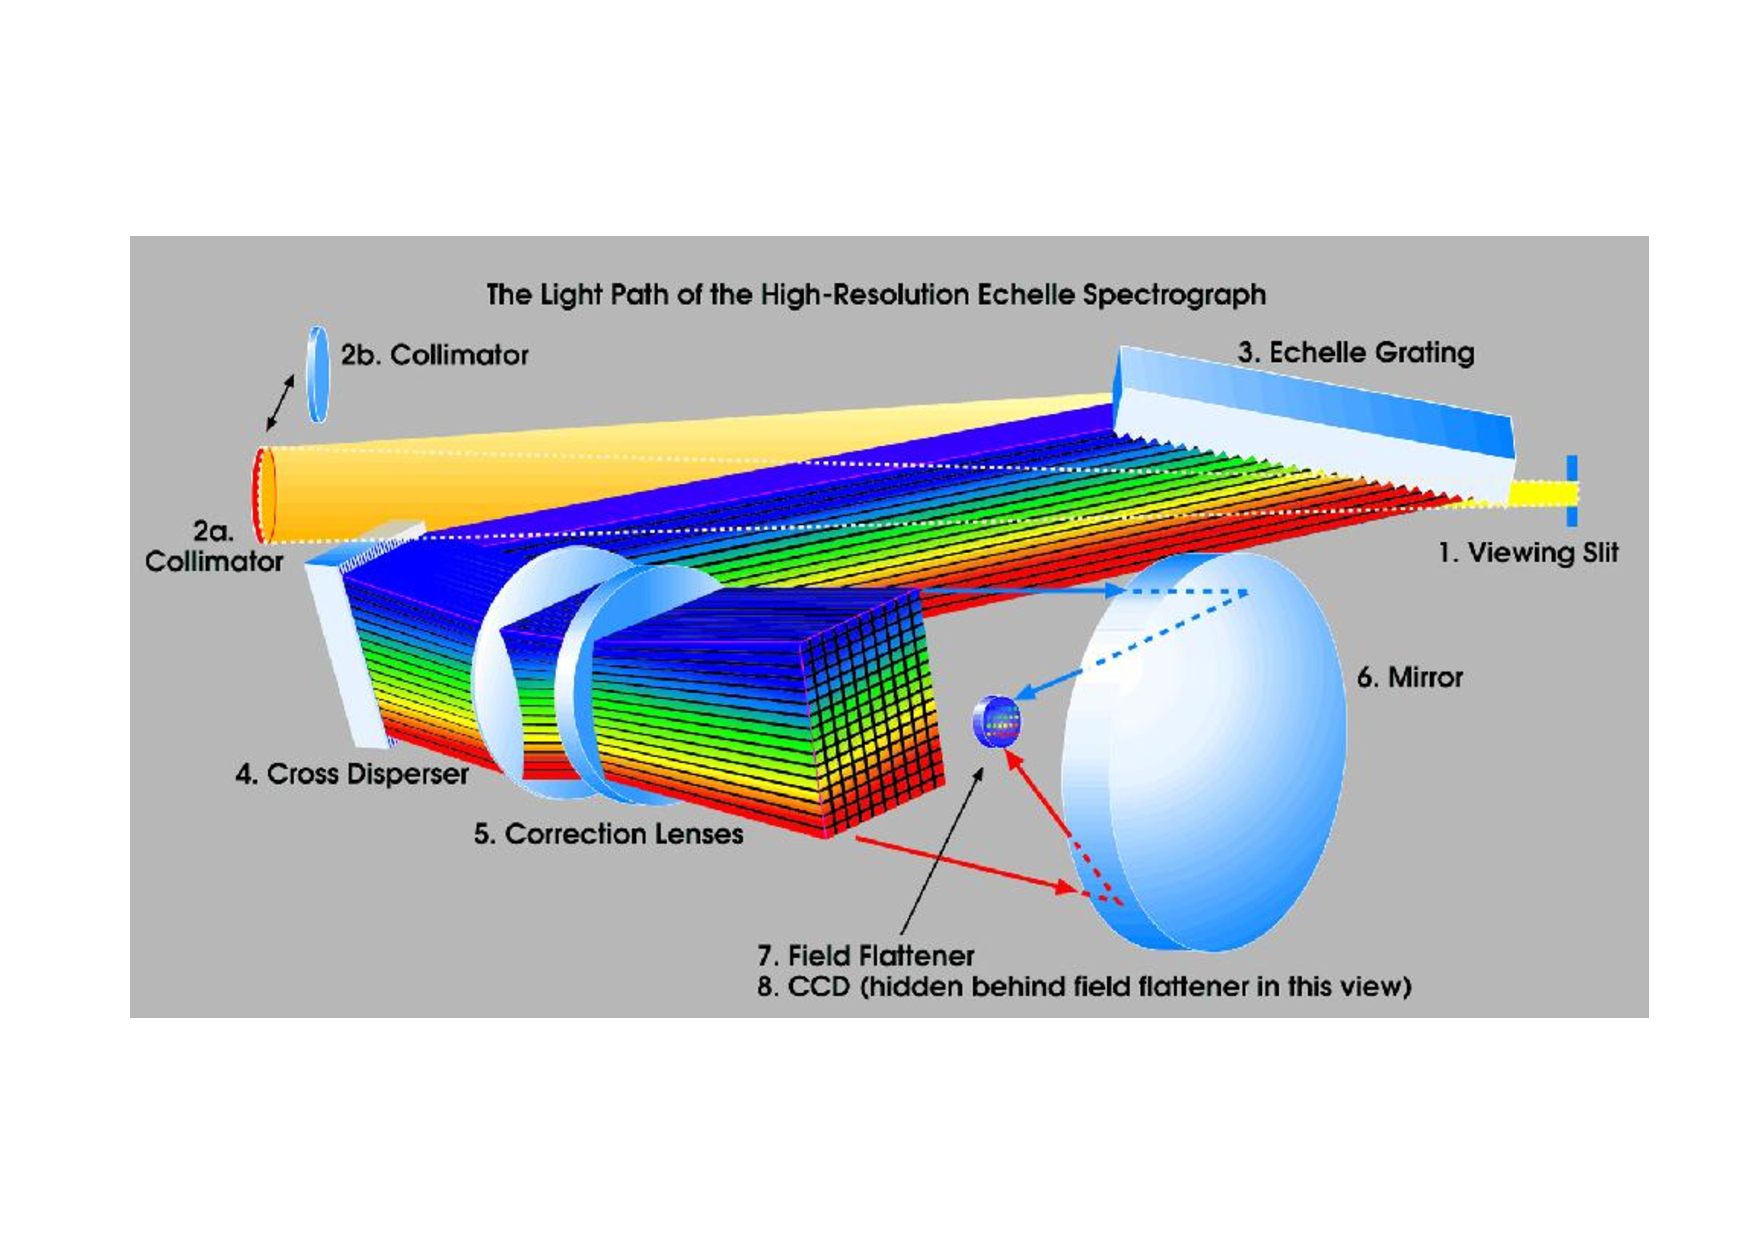
\includegraphics[scale=0.55]{Figures/4-Chromospheric_age/HIRES_diagram.pdf}
    \caption[Example of echelle spectrograph]{An example of an echelle spectrograph setup from \textit{Keck}. Image Credit: Keck / HIRES}
    \label{fig:echelle_diagram}
\end{figure}

An echelle spectrograph optimises the amount of CCD used by using an echelle grating to disperse the incoming light, an example of such a setup is shown in Figure \ref{fig:echelle_diagram}. The echelle grating has rulings that are much further apart than in typical gratings which allows for high dispersion but over a much shorter wavelength range. As the orders increase, there will be overlap in the wavelength range covered therefore a cross disperser is used to separate the orders in the focal plane. This setup allows for multiple orders to be imaged on a single CCD allowing for high-resolution spectra to be obtained.

\section{Observations}
\subsection{Sample selection}
\label{Chp4_obs_sample_selection}
The sample considered in this work were selected from stars studied by \citet{Bruntt_etal_2012}, who performed a detailed spectral study aided by asteroseismic data for 93 solar-type stars observed with \textit{Kepler}. For the purposes of studying the magnetic activity of old stars, the sample was restricted to stars with an outer convective envelope, are on the main sequence and have an asteroseismically determined age.

In order to select stars with an outer convective envelope, the effective temperature was required to be less than 6500 K, equivalent to spectral type F5V. Stars with spectral types earlier than F5V do not have a substantial outer convective envelope that is required for the solar-like dynamo process \citep{Pinsonneault_etal_2001}. Therefore, these stars are not expected to spin-down via magnetic braking during their main sequence lifetime or follow the same age-activity relationship as lower-mass stars. However, there is some observational evidence that hotter stars can occasionally display magnetic activity features as well; for example, weak X-ray emission was detected from the A7V star Altair \citep{Robrade_Schmitt_2009}. Therefore, data analysis was performed on all main sequence stars in the sample spanning the full effective temperature range of ca. 5000-6900 K, but stars with effective temperatures greater than 6500 K are displayed separately in tables and figures.

Stars that have significantly evolved off the main sequence are expected to have different rotational and magnetic evolution, therefore only stars that are still on the main sequence should be included in the age-activity analysis. To ensure that the stars in the sample were on the main sequence, their surface gravities \citep{Bruntt_etal_2012} from asteroseismology to the relation between $B-V$ colour and surface gravity for main sequence stars as given by \citet{Gray_2005} and shown in Equation \ref{Eq:Gray_2005}. Stars with surface gravities that differed by more than 0.2 dex were excluded from the sample.

Stellar ages from asteroseismology were collected from the literature. In particular, ages from \citet{Silva_Aguirre_etal_2017} were used for the majority of the sample, where stellar ages were obtained by modelling the individual oscillation frequencies in the spectrum observed by the \textit{Kepler} satellite. Some ages were also taken from \citet{Chaplin_etal_2014}, where stellar properties were estimated using two global asteroseismic parameters and complementary photometric and spectroscopic data.

\subsection{Spectra}
\label{Chp4_obs_spectra}
The spectra used in this study stem from \citet{Bruntt_etal_2012}. The spectra were obtained with the \esp spectrograph at the 3.6 m Canada-France-Hawaii Telescope (CFHT; \citealt{Donati_etal_2006}) and the \narval spectrograph \citep{Auriere_2003} mounted on the 2 m Bernard Lyot Telescope at the Pic du Midi Observatory. These spectra cover a spectral range of ${\thicksim} 3700$ to ${\thicksim} 10480$ \AA. In this work, the reduced spectra by \citet{Bruntt_etal_2012} was used which was received through personal communication. In \citet{Bruntt_etal_2012}, standard pipeline-reduced spectra were normalised using \texttt{RAINBOW} \citep{Bruntt_etal_2010} which allows manual normalisation of the spectra. The continua were adjusted by comparing with a synthetic spectrum and overlapping regions of spectral orders were checked so that both the line depths and continuum level matched.

Additional archival observations were used to investigate the level of long-term variability of the \Rprime indicator due to potential magnetic activity cycles (see Section REF). Pipeline-reduced spectra were obtained directly from the \esp archive\footnote{\url{http://www.cadc-ccda.hia-iha.nrc-cnrc.gc.ca/en/}}.

In the following sections (i.e Sections \ref{Chp4_data_analysis}, \ref{Chp4_results} and \ref{Chp4_discussion}), the focus will be on the data analysis, results and discussion of the chromospheric emission from the \caII spectral lines.

\section{Data Analysis}
\label{Chp4_data_analysis}

In this section, the process to extract the chromospheric emission from the \caII lines is described. It details the processing of the spectra data, the calibration of the emission to the Mount Wilson S index and how the final \Rprime indicator value was calculated. Section \ref{Chp4_halpha} will discuss the analysis performed on the H-$\alpha$ spectral line.

\subsection{Doppler correction}
\label{Chp4_data_analysis_doppler}
The first step in the data analysis was to correct for any Doppler shift present in the stellar spectrum. Doppler shifts in spectra are a common occurrence in astronomical spectra due to the relative motions of stars and is seen as a change in the wavelength that spectral lines are observed at. Since the relative motions of each of the stars is slightly different, then the core of the \caII lines (where the chromospheric emission is observed) will be observed at slightly different wavelengths. In order to analyse the correct part of the spectral lines the Doppler shift must be accounted for; this is achieved by comparing all spectra to one master spectrum and adjusting the wavelength scale so that spectral line coincide at the same wavelength.

A master spectrum was selected by considering the signal to noise ratio (hereafter SNR) in the 3850 to 4050 \AA wavelength region. The SNR was calculated using Equation \ref{Eq:SNR_ratio} where $\bar{f}$ is the mean flux value and $\sigma_{f}$ is the standard deviation of the flux in the relevant wavelength region. The spectrum with the largest SNR value was chosen as the master spectrum to which all other spectra were compared to; the master spectra were KIC 9226926 and KIC 3733735 for the \narval and \esp spectra, respectively.

\begin{equation}
SNR = \frac{\bar{f}}{\sigma_{f}}
\label{Eq:SNR_ratio}
\end{equation}

A cross correlation function was then used to compare each of the spectra to the master spectrum; this function measures the similarity of a spectrum to the master spectrum as a function of the relative displacement. The maximum of the cross correlation function was then used to determine the relative displacement that must be taken into account for the two spectra to be aligned. The relative displacement was applied to the spectrum, allowing analysis of the \caII lines using the same wavelength regions for all spectra. An additional manual wavelength correction was applied to the spectra in order to to compensate for any Doppler shift that was present in the master spectrum. This was $-0.2$ \space \AA for the \esp data; the \narval data did not require this manual correction.

An additional analysis was also performed to check for any nominal negative flux values in the core of the \caII lines. While negative flux values are not physically real, they can be caused by the automatic pipeline reduction performed on the spectra. Particularly since the \caII lines are located at the blue end of the spectrograph. Any spectra with negative flux values in the \caII cores were excluded from the analysis.

\subsection{Normalisation of continuum}
\label{Chp4_data_analysis_normalise_cont}
Before the \Rprime indicator could be calculated, the spectra were required to be normalised as there was a discontinuity in the continuum at the \caII wavelengths. This is shown in the top panel of Figure \ref{fig:normlisation_example}; the flux in the overlapping region match reasonably well, but the continuum level flux level is higher in the K order than the H order. This would have an effect on the chromospheric emission measurement as the method used (see Section \ref{Chp4_data_analysis_calc_S}) requires the flux measured in the core of the \caII lines to be normalised by the flux continuum in two reference channels.

\begin{figure}
    \centering
    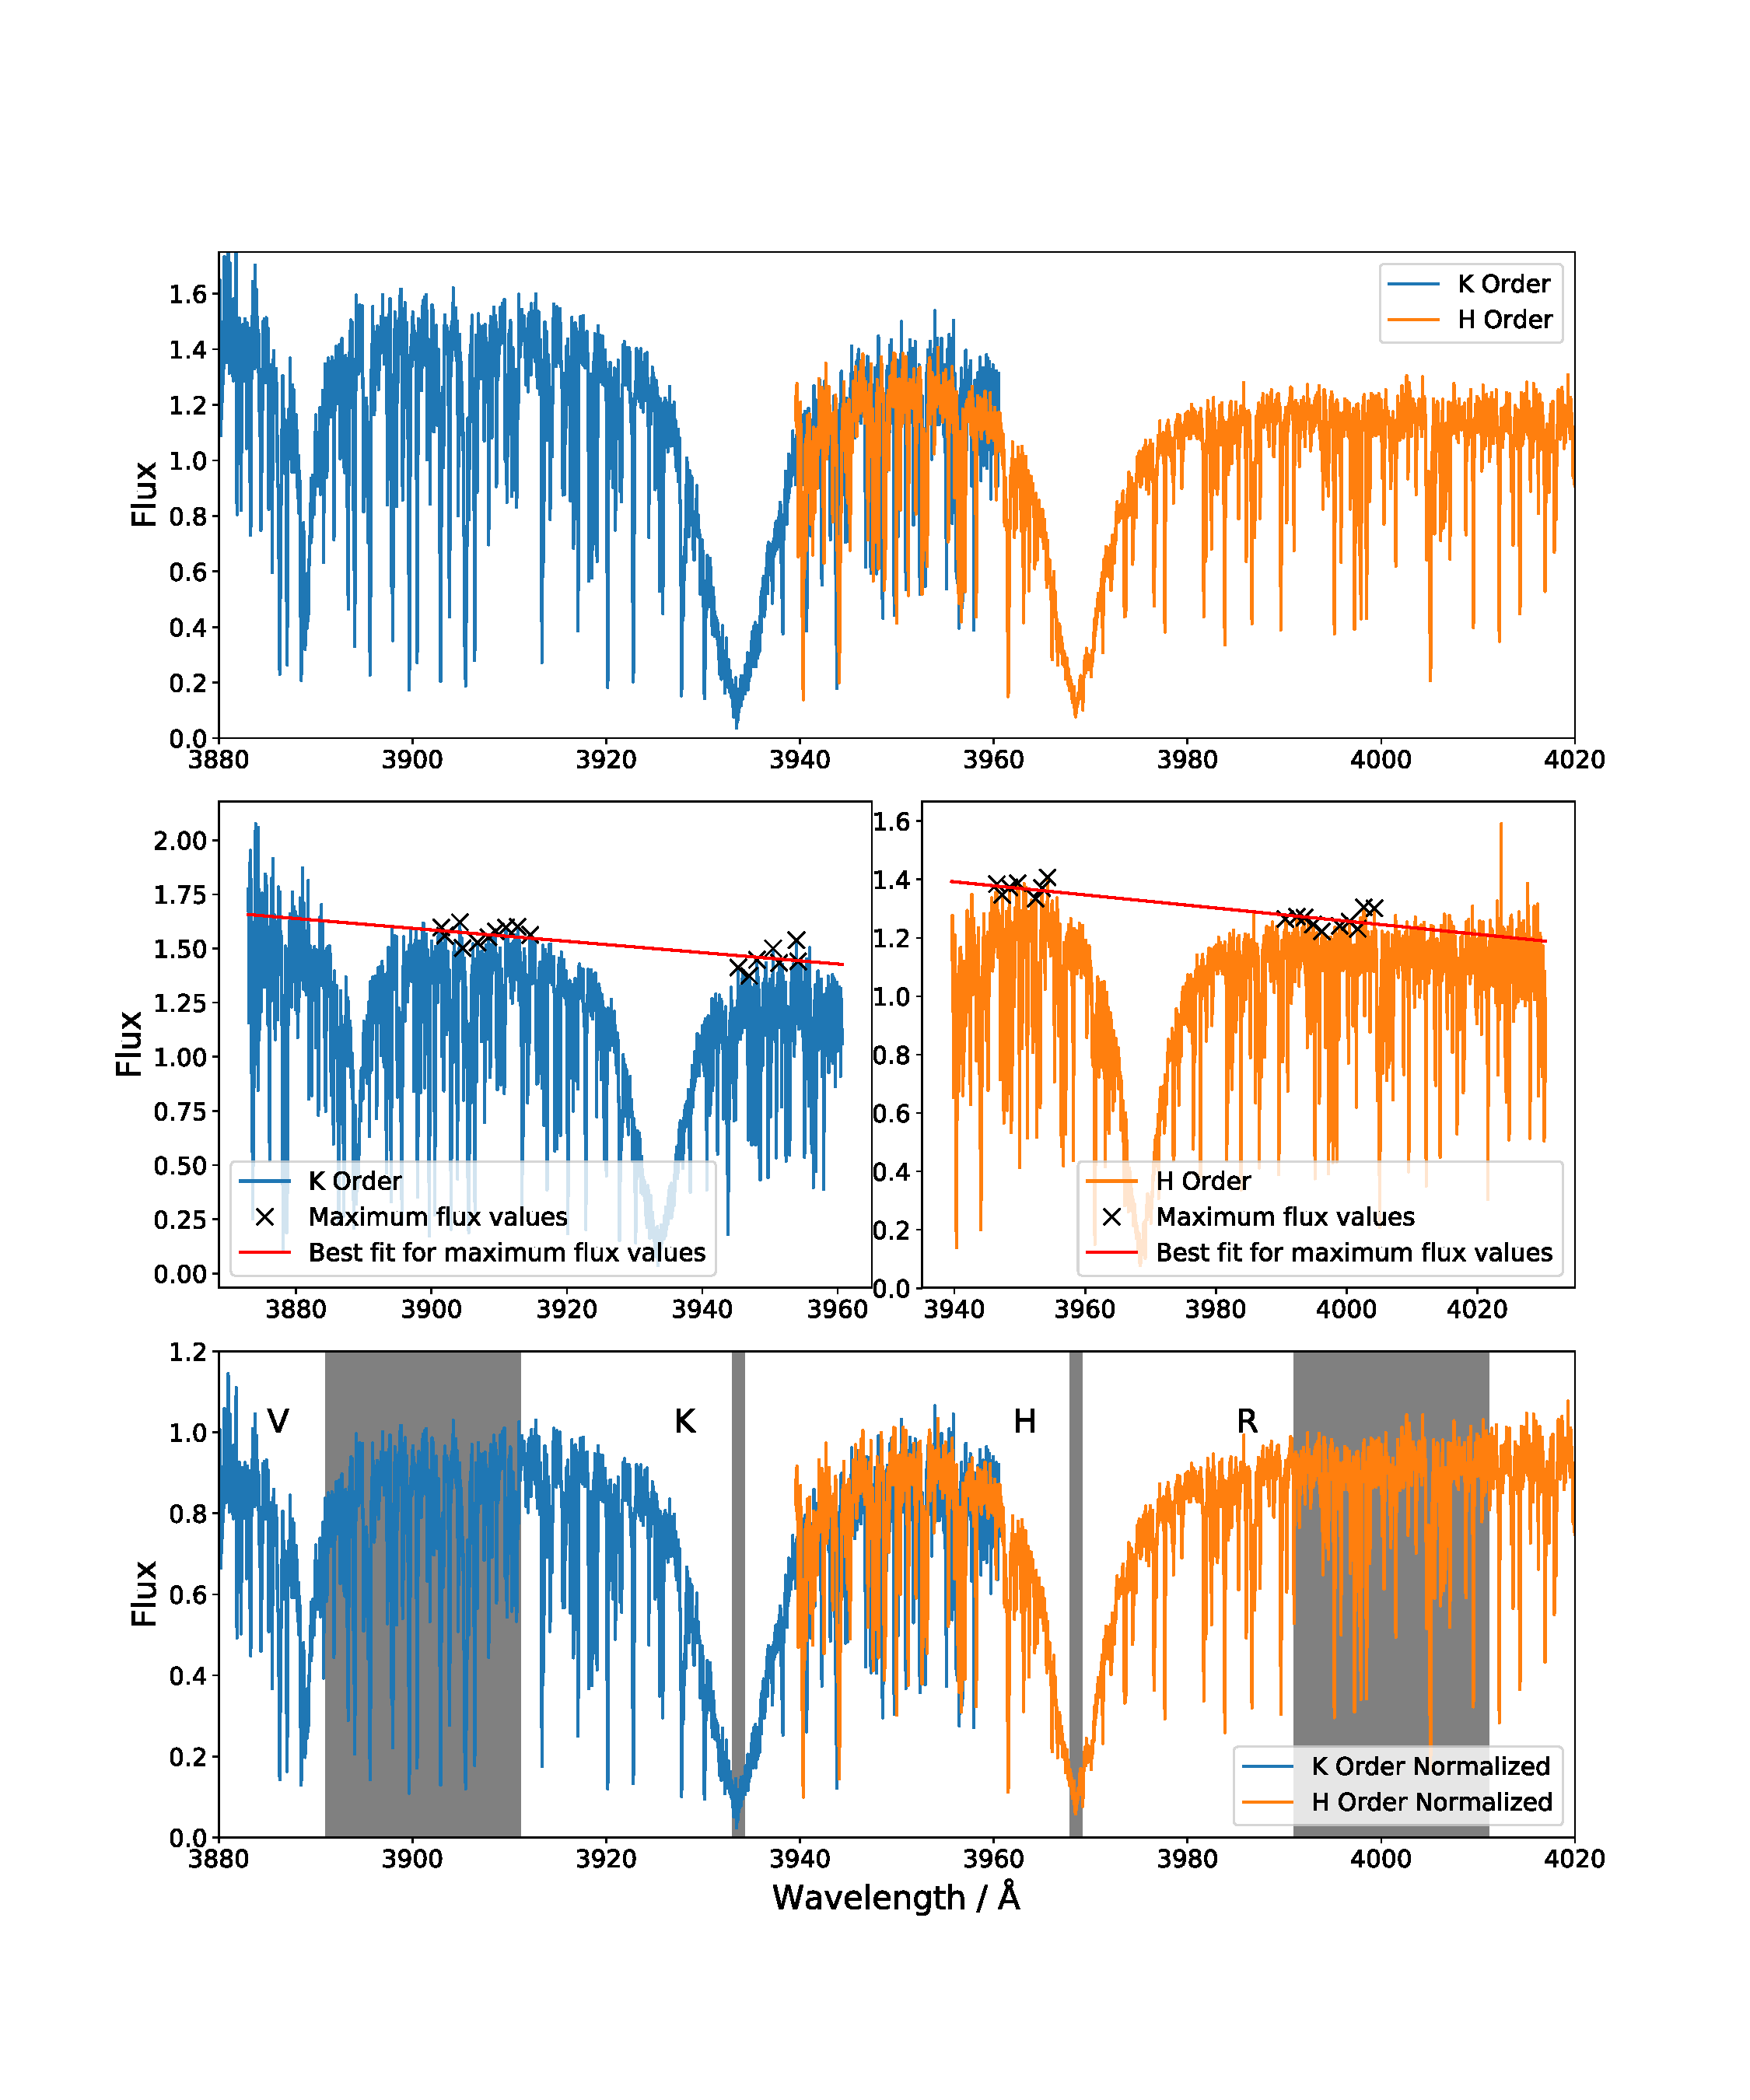
\includegraphics[scale=0.40]{Figures/4-Chromospheric_age/kic9139163_example.pdf}
    \caption[Example of optical spectra in \caII region and the normalisation method]{\textbf{Top panel:} Spectrum of KIC 9139163 showing the two adjacent spectral orders that contain the \caII lines. While the overlapping region of the orders match, there is a clear discontinuity in the continuum flux level.
    \textbf{Middle panel:} Plots of the two comparison regions in the K order (left) and H order (right). The markers denote the maximum flux values in each bin of width 1.5 \AA. The red line denotes the best-fitting linear relationship that is used to normalise the spectrum.
    \textbf{Bottom panel:} Spectrum of KIC 9139163 with correction factor applied to the K order. The discontinuity in the continuum flux level is no longer present. The four channels used to calculate the S index are also shown.}
    \label{fig:normlisation_example}
\end{figure}

This was corrected by considering two comparison regions in each spectral order; from 3900 - 3915 \AA \space and 3945 - 3955 \AA \space in the shorter-wavelength order of the spectrum (containing the Ca~II K line) and from 3945 - 3955 \AA \space and 3990 - 4005 \AA \space in the longer-wavelength order of the spectrum (containing the Ca~II H line) as shown in the middle panel of Figure \ref{fig:normlisation_example}. The local continuum level was estimated in those regions by splitting the spectrum into bins of 1.5 \AA \space width and measuring the local maximum in each of the bins (see Figure \ref{fig:normlisation_example}). These data points were used to find the best-fitting linear relationship as indicated by the red line in the middle panel of Figure \ref{fig:normlisation_example}. The spectra were then normalised according to this best fitting relationship so that the typical continuum flux value in each order was approximately one.

\subsection{Calculation of S index}
\label{Chp4_data_analysis_calc_S}
The S index is an activity indicator that uses four channels to quantify the chromospheric emission in the core of the \caII lines. Two channels are 1.09 \AA \space wide and centred on 3968.47 and 3933.664 \AA \space for the \caII cores, respectively. The other two channels are 20 \AA \space wide and are centred on 3901.07 and 4001.07 \AA; named the V and R channels respectively. These channels are shown in the bottom panel of Figure \ref{fig:normlisation_example} and follow the channels defined by \citet{Lovis_etal_2011} with the exception that the triangular-shaped profile to the H and K channels are not included in this analysis.

The S index is calculated using Equation \ref{Eq:sindex} where $N_{x}$ is the total flux in the relevant channel. The error associated with $N_{x}$ is calculated using Equation \eqref{Eq:sindex_error} where $x_{n}$ is the error on the individual flux data point and $i$ is the total number of data points in the wavelength channel. These errors associated with $N_{x}$ were then propagated in order to calculate the error associated with the S index.

\begin{equation}
S = \frac{N_{H} + N_{K}}{N_{R} + N_{V}}
\label{Eq:sindex}
\end{equation}

\begin{equation}
\sigma_{N_{x}} = \sqrt{\sum_{n=1}^{i} x_{n}^{2}}
\label{Eq:sindex_error}
\end{equation}


\subsection{Calibration to \texorpdfstring{\Smw}{Smw} and calculating the \texorpdfstring{\Rprime}{Rprime} indicator}

\begin{figure}
    \centering
    \begin{subfigure}{\textwidth}
        \centering
        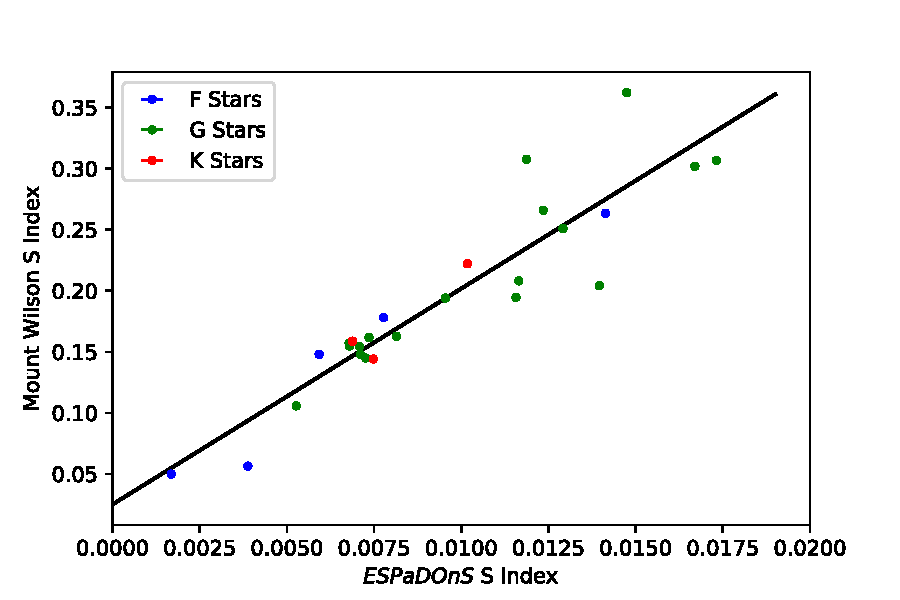
\includegraphics[scale=0.75]{Figures/4-Chromospheric_age/espadons_calibrator_reltionship.pdf}
        \caption{\esp Calibrators}
    \end{subfigure}
    \begin{subfigure}{\textwidth}
        \centering
        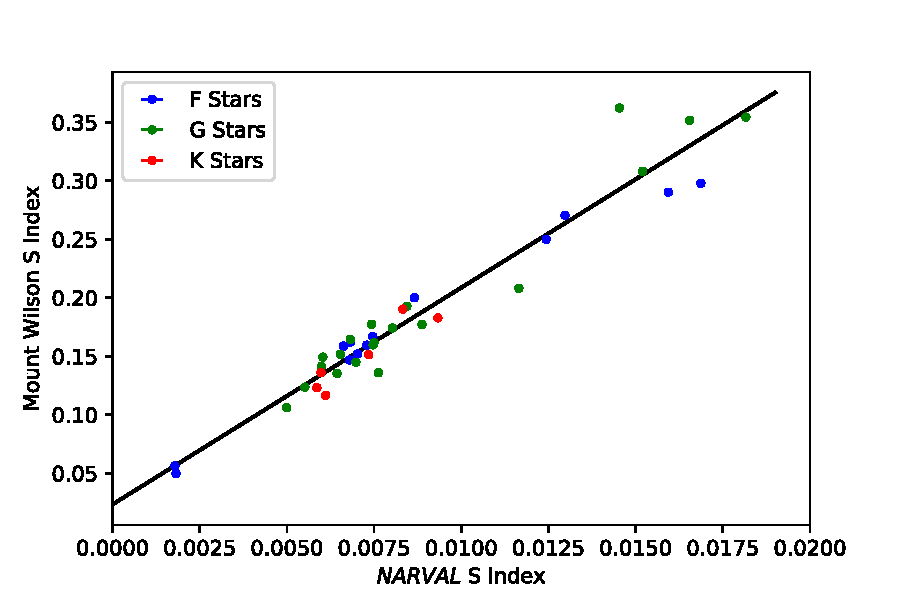
\includegraphics[scale=0.75]{Figures/4-Chromospheric_age/narval_calibrator_reltionship.pdf}
        \caption{\narval Calibrators}
    \end{subfigure}
    \caption[Calibration relationships to \Smw]{Plots showing the average \Smw \citep{Duncan_etal_1991} against the S index calculated from the \esp/\narval spectrographs for the calibrator stars. The black line indicates the best-fitting linear relationship between the two parameters.}
    \label{fig:calibrator_relationships_Smw}
\end{figure}

The method that is used to calculate the \Rprime indicator (\citealt{Noyes_etal_1984}; see Section \ref{chromospheric_emission_subsub}) requires the Mount Wilson S index (\Smw), which differs slightly from the S index calculated for the sample of stars considered in this work. The S index calculated in any spectrum (regardless of the exact method used) is dependent on the spectral resolution and the throughput of the spectrograph used. therefore it was necessary to determine a relationship between the S index calculated from the spectrographs used in this work (\esp and \narval) and \Smw. This was achieved by searching for stars from \citet{Duncan_etal_1991} in the \esp and \narval archives. \citet{Duncan_etal_1991} summarises measurements of \caII emission at the Mount Wilson Observatory from 1966 - 1983, thus providing a large sample of stars with measured \Smw values. The comparison sample was restricted to have the same range of spectral type as used in the analysis of old inactive stars, i.e. from spectral type F5 to late K. The stars from \citet{Duncan_etal_1991} with archival observations from \esp and \narval were Doppler corrected and normalised using the sample method as the main sample (see Section \ref{Chp4_data_analysis_doppler} and \ref{Chp4_data_analysis_normalise_cont}). The master spectra for Doppler correction were HD 89449 and HD 126660 for \esp and \narval data, respectively. The manual wavelength shift was -0.14 and +0.1 \AA \space for the \esp and \narval data, respectively. The full list of stars and values used to calibrate the two relationships are shown in Appendix \ref{App_calibrator_stars_Smw}.

The S index was calculated for these calibrator stars as described in Section \ref{Chp4_data_analysis_calc_S} and plotted against the mean \Smw from \citet{Duncan_etal_1991} (shown in Figure \ref{fig:calibrator_relationships_Smw}). Since the sample considered in this work contains weakly inactive stars older than a gigayear, we restricted the calibrator star sample to S index values less than 0.2 and \Smw values less than 0.5. A linear least-squares regression was applied to the data to find the best-fitting relationship between the two indices, which are shown in Equations \ref{Eq:esp_calibrator_eq} and \ref{Eq:nar_calibrator_eq}. These equations were used to calculate the \Smw for our sample of stars with asteroseismic ages.

\begin{equation}
S_{MW} = 17.67 \cdot S_{\mathrm{ESPaDOnS}}+ 0.025
\label{Eq:esp_calibrator_eq}
\end{equation}

\begin{equation}
S_{MW} = 18.53 \cdot S_{\mathrm{NARVAL}} + 0.023
\label{Eq:nar_calibrator_eq}
\end{equation} 

Using the \Smw values calculated from the calibration relationships, the \Rprime indicator was calculated using the original method by \citet{Noyes_etal_1984} (see Section \ref{chromospheric_emission_subsub}).

\subsection{Analysis using two channels}
\label{Chp4_data_analysis_two_channel}
Additional observations were searched for in the \esp archive in order to investigate the effect of potential magnetic activity cycles on the value of the \Rprime indicator (see Section REF). However, a significant number of spectra taken from the \esp archive contained strong scatter in the spectral order where the Ca II K line is located, whereas the scatter was much lower in the spectral order containing the Ca II H line. Therefore, a modified S index and \Rprime indicator using only the H and R channels was calculated. Specifically, the modified S index was calculated using Equation \ref{Eq:modified_S} where $N_{x}$ is the total flux in the relevant channel.

\begin{equation}
    S_{mod} = \frac{N_{H}}{N_{R}}
    \label{Eq:modified_S}
\end{equation}

Since the Ca II H typically shows slightly less of a flux excess in the line centre than the K line, a new \Smw calibration was performed for the modified S index using the calibrator stars from \citet{Duncan_etal_1991}. The best-fitting relationships for the modified S index and average \Smw value for each spectrograph are shown in Equation \ref{Eq:esp_calibrator_eq_mod} and \ref{Eq:nar_calibrator_eq_mod}. Once the Mount Wilson S value has been found, the conversion to the \Rprime indicator is identical to the four channel method.

\begin{equation}
S_{MW} = 21.93 \cdot S_{\mathrm{ESPaDOnS (mod)}}+ 0.016
\label{Eq:esp_calibrator_eq_mod}
\end{equation}

\begin{equation}
S_{MW} = 21.79 \cdot S_{\mathrm{NARVAL (mod)}} + 0.014
\label{Eq:nar_calibrator_eq_mod}
\end{equation} 

\section{Results}
\label{Chp4_results}

\subsection{Calcium chromospheric emission with age}
\label{Chp4_results_general_results}
The chromospheric emission from \caII lines was measured for a sample of 26 stars with asteroseismic ages. The sample contains primarily F and G stars, as well as one K star.

In Figure \ref{fig:calcium_emission_plot}, the \Rprime activity indicator is plotted as a function of stellar age. The data points are colour-coded according to their spectral type; G and K stars are displayed in green and orange, respectively, while mid to late F stars (with effective temperatures below 6500 K) are displayed in blue. Earlier F stars with effective temperatures between 6500 K and 6900 K are displayed in red; these stars are separated from the later F stars due to the very thin outer convective zone present in these earlier type stars and thus are not expected to spin down in the same manner as the rest of the sample.

\begin{figure}[h]
	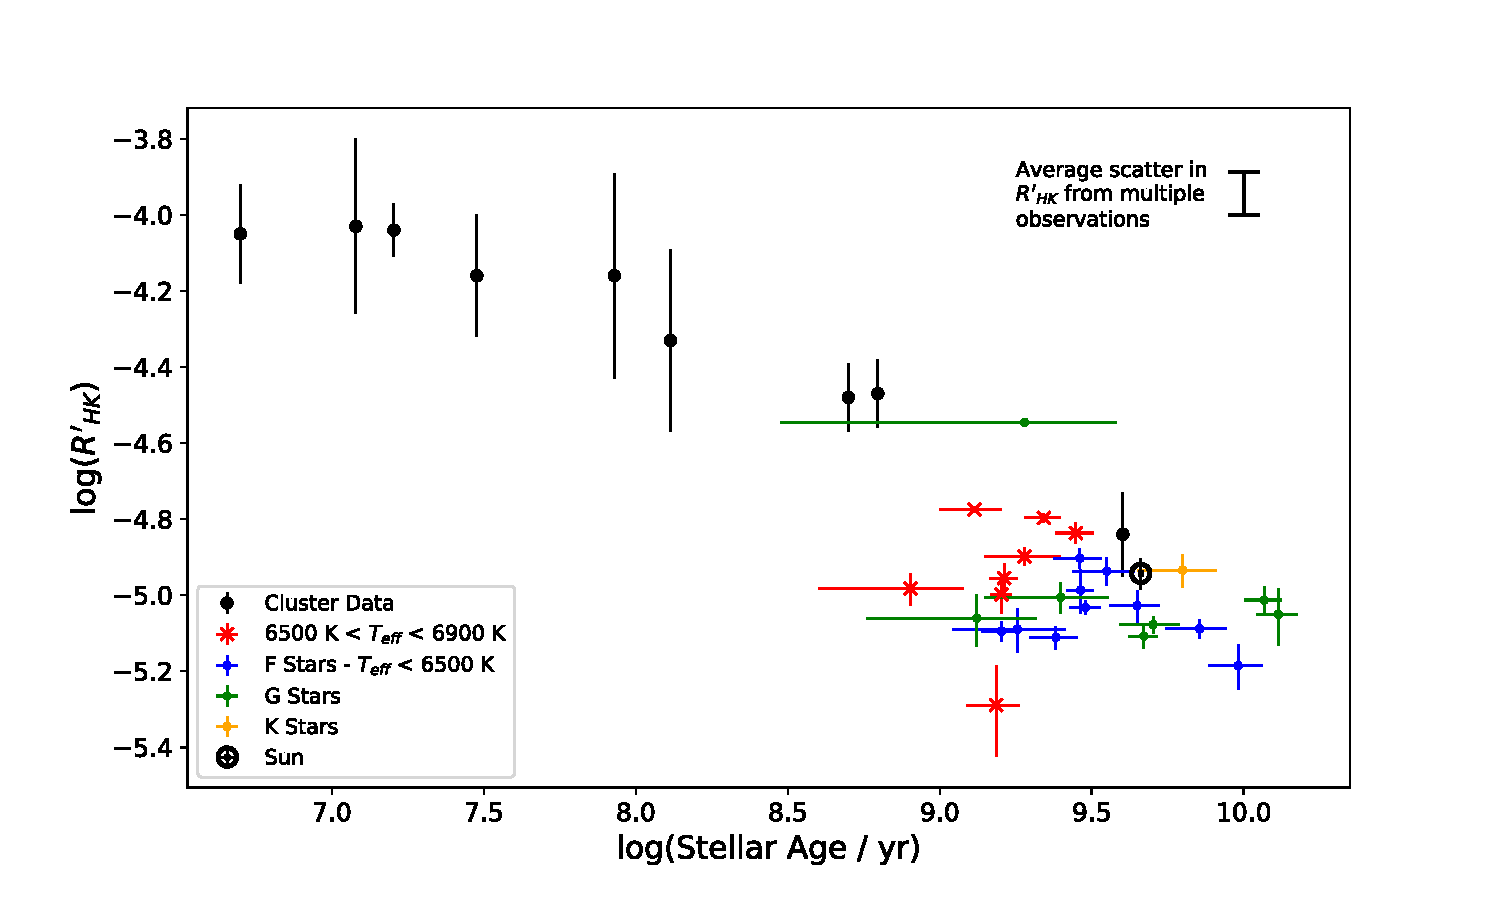
\includegraphics[width=0.99\textwidth]{Figures/4-Chromospheric_age/ca_results_with_clusters.pdf}
	\caption[Calcium emission as a function of age for sample and cluster data]{Plot showing data analysed in this work alongside cluster data from \citet{Mamajek_Hillenbrand_2008} shown in black. The average solar value over several cycles is also shown \citep{Egeland_etal_2017}.}
	\centering
	\label{fig:calcium_emission_plot}
\end{figure}

The full details for each star are given in Appendix \ref{App_calcium_results}. Three stars (KIC 5774694, KIC 9139163 and KIC 10454113) had observations from both of the spectrographs considered in this work (\esp and \narval). For simplicity, only the \narval data for these stars are shown in Figure \ref{fig:calcium_emission_plot} as these have smaller associated errors in the activity measurement. 

To set the data for the old stars into context, the typical spread in chromospheric activity for a sample of young stellar clusters and M67 are shown in Figure \ref{fig:calcium_emission_plot}. This cluster data is taken from Table 6 of \citet{Mamajek_Hillenbrand_2008} with errors representative of the 68\% confidence level. \citet{Mamajek_Hillenbrand_2008} collected stellar \Rprime indicator values from the available literature in a colour range of B-V = 0.46 to 0.89, which corresponds to effective temperatures of 5000 - 6500 K and matches closely to the sample selection of K, G and mid-to-late F dwarfs considered in this work. For further comparison, the mean \Rprime value for the Sun over several cycles is also shown \citep{Egeland_etal_2017}. The age of the Sun is taken to be $4.57 \pm 0.02$ Gyr \citep{Bahcall_etal_1995}.

Figure \ref{fig:calcium_emission_plot} shows that the scatter in the \Rprime activity measurements for the old stars considered in this work is quite large. Setting the F stars with effective temperatures grater than 6500 K aside, our stars span a range of \Rprime values between $-4.5<\mathrm{log}(R^{'}_{HK})<-5.2$. One star in the sample, the G dwarf KIC 5774694, has an unusually large \Rprime value; it is also a star with a large uncertainty in its asteroseismic age. Unfortunately, only a single epoch of an activity measurement is available for this star so we cannot test if a stellar flare temporarily increased the activity of this star. Therefore, if this G dwarf is considered a potential outlier with respect to activity or age, the range of activity values displayed by the mid-F to K dwarf sample is $-4.85<\mathrm{log}(R^{'}_{HK})<-5.2$.

The activity data points for the sample of old stars considered in this work do not seem to display a strong trend with stellar age. To quantify this, Spearman's rank coefficient was calculated for the sample. The Spearman's rank coefficient ($\rho$) is a parameter-free correlation indicator and is calculated using Equation \ref{Eq:spearman_rank_coeff} where $d_{i}$ is the difference in rank between the two parameters and $n$ is the number of data points. More importantly, the Spearman's rank coefficient is independent of any specific functional form of the correlation between the two quantities. A value of 0 implies no correlation, 1 implies perfect correlation, and -1 implies perfect anticorrelation. For chromospheric activity and stellar age in the mid-F to K dwarf sample in this research, the Spearman's rank coefficient is found to the -0.038, implying that basically no correlation is present in the data.

\begin{equation}
    \rho = 1 = \frac{6\Sigma d_{i}^{2}}{n(n^{2}-1)}
    \label{Eq:spearman_rank_coeff}
\end{equation}

\subsection{Comparison with M67}
The M67 cluster has an age of $\sim 4$\,Gyr \citep{Demarque_etal_1992,VandenBerg_Stetson_2004,Bellini_etal_2010} and the chromospheric activity of ca. 70 of its member stars have been reported in the literature \citep{Giampapa_etal_2006,Mamajek_Hillenbrand_2008}. The cluster is well-studied and measurements of the stellar rotation periods make it a benchmark for the spin down of cool stars \citep{Barnes_etal_2016}. It is a useful comparison target to our old-star sample and it is displayed in Figure \ref{fig:calcium_emission_plot} as part of the \citet{Mamajek_Hillenbrand_2008} cluster data.

Surprisingly, we find that the chromospheric activity of the M67 stars is higher than what is seen in our sample of stars for similar ages. It is important to note that \citet{Mamajek_Hillenbrand_2008} calculated the \Rprime values from the measurements performed by \citet{Giampapa_etal_2006}, who studied only G-type stars in their work. So the appropriate comparison group is the old G stars in our sample, i.e. the green data points in Figure \ref{fig:calcium_emission_plot}. There the discrepancy is even more pronounced: we see that the M67 stars display an activity level roughly 0.2 dex higher than the G stars with a similar age in our sample.

Therefore, an additional analysis was performed to see if data reduction issues could be the reason for this discrepancy. To this aim, additional spectra for member stars of the three oldest clusters from \citet{Mamajek_Hillenbrand_2008}, i.e. M67, the Ursa Major (UMa) moving group and the Hyades, in the \esp and \narval archives. Unfortunately no archival observations of M67 member stars were found, however, spectra of five UMa member stars and two Hyades member stars were found. Using the two channel analysis as described in Section \ref{Chp4_data_analysis_two_channel}, the spectra were analysed to obtain the \Rprime indicator. These values for the \Rprime indicator were plotted as a function of age and compared to the \citet{Mamajek_Hillenbrand_2008} values for the cluster as shown in Figure \ref{fig:cluster_data_comparison}. 

Figure \ref{fig:cluster_data_comparison} shows that there is some scatter in the \Rprime values found from archival observations, which is to be expected given the intrinsic stellar variability of cool stars. However, there is one star that has an extremely low value for the \Rprime indicator, HD 38393. It's value for the \Rprime activity indicator is more in line with what we would expect from our old field star sample. In \citet{Mamajek_Hillenbrand_2008}, HD 38393 had measured values for the \Rprime activity indicator of $-4.77$ and $-4.82$. Upon further investigation, we found that this is classed as a double star on SIMBAD, therefore this may effect the value of the \Rprime activity indicator. With the exception of this outlier, the archival observations from \esp and \narval are in agreement with the \citet{Mamajek_Hillenbrand_2008} values. No systematic offset exists between the two data sets; therefore the difference in the activity levels between the asteroseismic sample and the cluster sample is real and discuss the possible explanations for this discrepancy in Section REF.

\begin{figure}
    \centering
    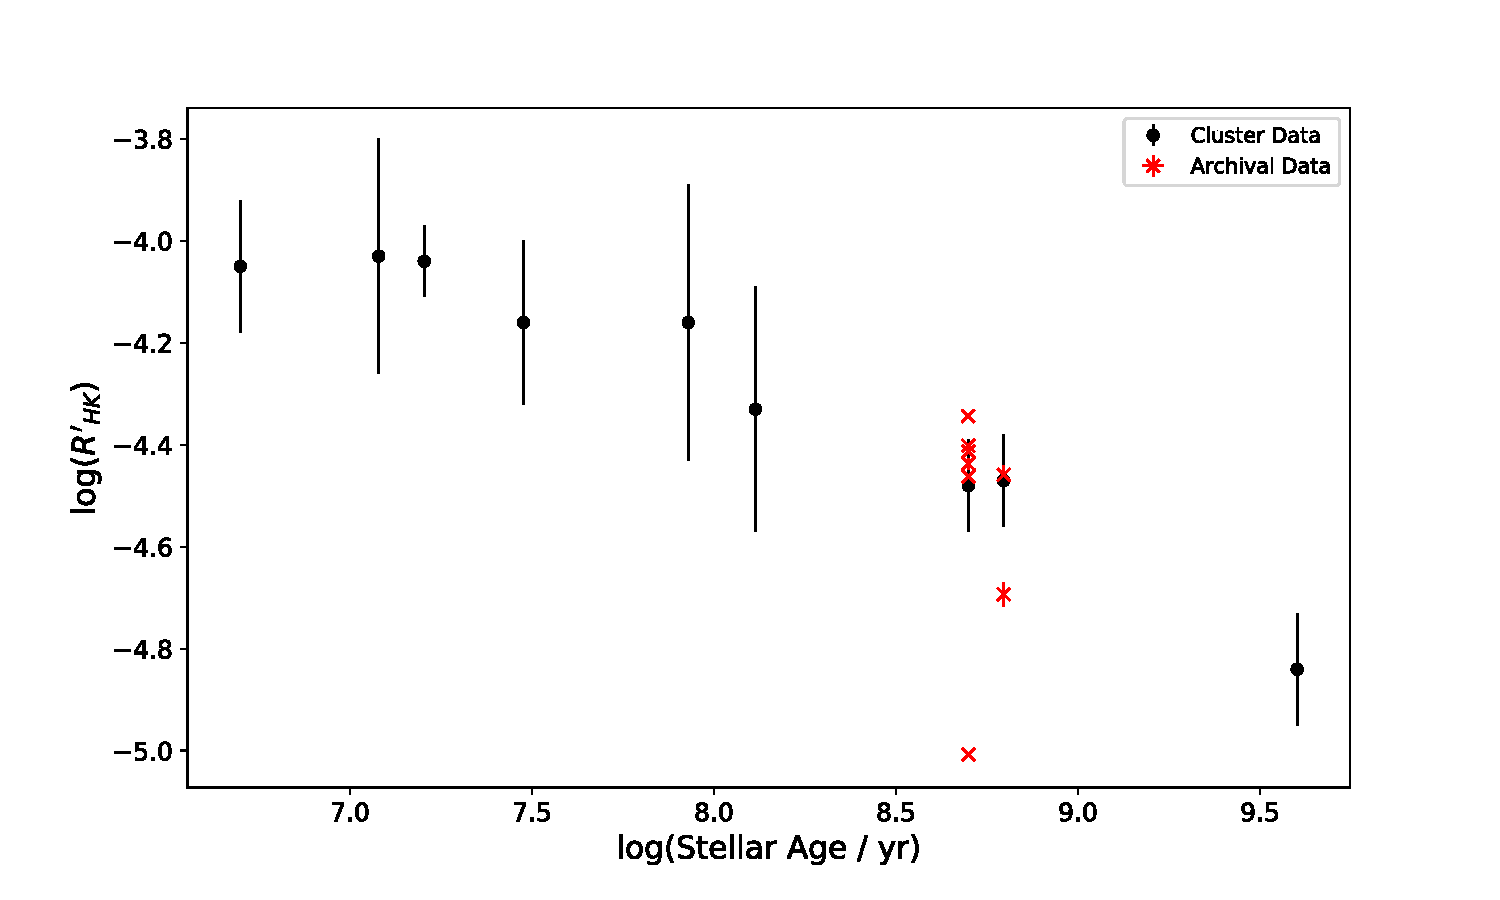
\includegraphics[scale=0.5]{Figures/4-Chromospheric_age/cluster_data.pdf}
    \caption[Analysis of cluster members]{Plot of cluster data from \citet{Mamajek_Hillenbrand_2008} alongside archival data from \esp and \narval of Ursa Major moving group and Hyades members.}
    \label{fig:cluster_data_comparison}
\end{figure}

\subsection{Variability of stars}
It is known that cool stars may have magnetic activity cycles similar to the solar eleven year activity cycle \citep{Wilson_1978,Baliunas_etal_1995}. Therefore, an investigation into the activity spread due to intrinsic stellar variability, i.e. by sample stars being in different stages of a possible activity cycle, was also conducted. The \esp and \narval archives were searched for additional observations of the sample of stars with asteroseismic ages. Thirteen of the sample stars had been observed with \esp at additional epochs. Seven of those stars are mid-F to K stars and six are hotter F stars. The details of these observations are shown in Table \ref{Table:esp_additional_obs_table}. Note that no additional observations were found in the \narval archive.

\begin{table}
\centering
\begin{tabular}{lclc}
\hline
Star Name    & Year & Product ID & Integration Time / s \\
\hline
KIC 2837475  & 2014 & 1733329i   & 145                  \\
KIC 2837475  & 2015 & 1818237i   & 78                   \\
KIC 3733735  & 2015 & 1818236i   & 70                   \\
KIC 6106415  & 2014 & 1740569i   & 60                   \\
KIC 6225718  & 2014 & 1740585i   & 60                   \\
KIC 8694723  & 2014 & 1733346i   & 255                  \\
KIC 9139151  & 2014 & 1733349i   & 280                  \\
KIC 9206432  & 2014 & 1740570i   & 250                  \\
KIC 9226926  & 2014 & 1721307i   & 210                  \\
KIC 9955598  & 2013 & 1630041i   & 1700                 \\
KIC 10454113 & 2014 & 1733354i   & 165                  \\
KIC 10454113 & 2016 & 2005115i   & 840                  \\
KIC 10709834 & 2015 & 1791287i   & 262                  \\
KIC 10963065 & 2013 & 1628074i   & 1625                 \\
KIC 11253226 & 2014 & 1740580i   & 140					\\
\hline
\end{tabular}
\caption[Details of archival \esp observations]{Details of observations taken from \esp archive to sample potential magnetic activity cycles present.}
\label{Table:esp_additional_obs_table}
\end{table}

Due to the scatter in the spectral order containing the Ca II K order in archival observations, the analysis of the chromospheric emission was conducted using the two channel method described in Section \ref{Chp4_data_analysis_two_channel}. The results of the additional observations are shown in Appendix \ref{App_ca_multiple_obs_tables}. The results of these additional observations along with the original observation for the relevant stars ($T_{eff} < 6500$ K) are shown as a function of their age in Figure \ref{fig:ca_multiple_obs}. Solar values are also shown for reference \citep{Egeland_etal_2017}. The corresponding plot for the hotter F stars is shown in Figure \ref{fig:ca_multiple_obs_hot_Fstars}. Note that the \Rprime indicator values were recalculated for the original observations using only the H and R channels for consistency, this modified activity versus age plot is shown in Appendix \ref{App_two_channel_plot}. The grey regions in Figures \ref{fig:ca_multiple_obs} and \ref{fig:ca_multiple_obs_hot_Fstars} indicated the activity region that the sample of stars occupy in the age-activity plot as determined from Figure \ref{fig:modified_ca_age_activity_plot_2channel}.

\begin{figure}
    \centering
    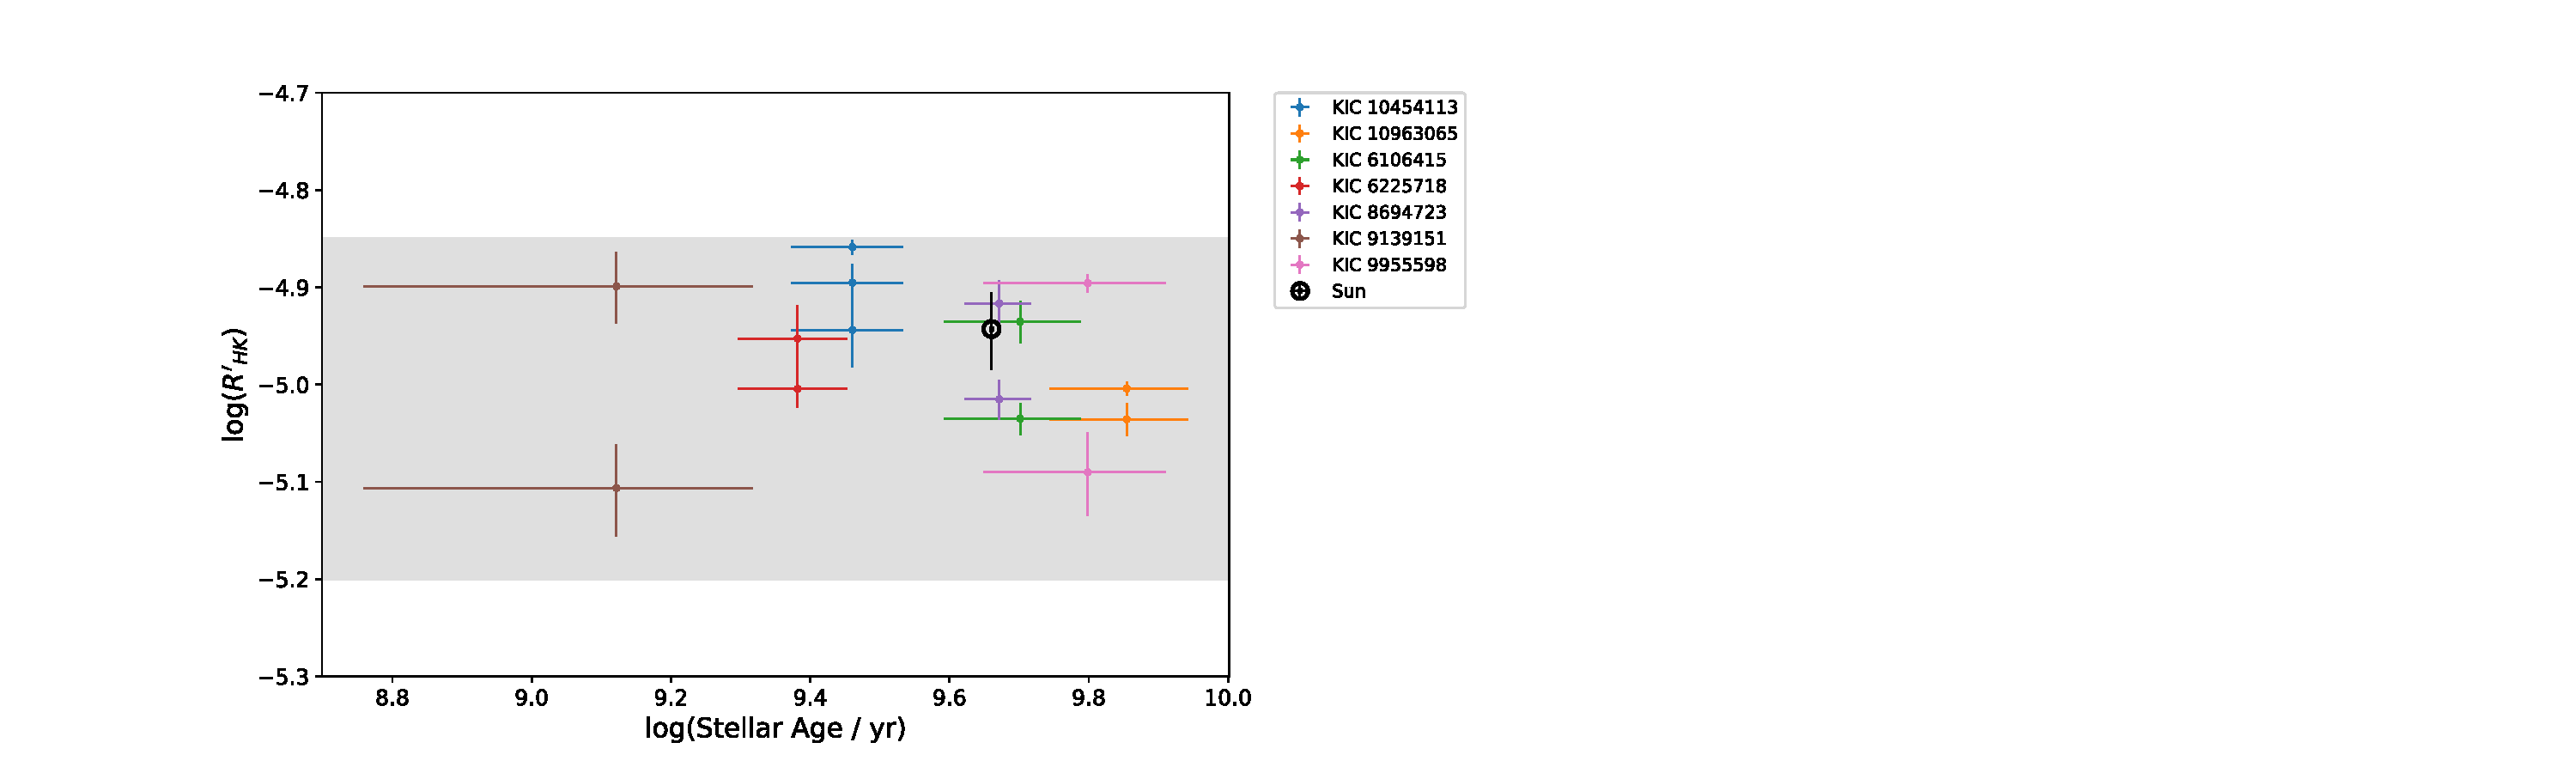
\includegraphics[scale=0.55]{Figures/4-Chromospheric_age/cool_multiple_obs_plot_with_sun.pdf}
    \caption[Plot showing activity over several epochs for stars with $T_{eff} < 6500$ K]{Plot showing the \Rprime indicator values calculated using only the H and R channels (see Section \ref{Chp4_data_analysis_two_channel} for further details) for multiple observations of stars in our sample ($T_{eff} < 6500$ K). The grey shaded region indicates the range of the \Rprime indicator values that our sample have when the \Rprime indicator is calculated using only the H and R channels (see Appendix REF for plot). The average solar value over several cycles \citep{Egeland_etal_2017} is also shown for reference.}
    \label{fig:ca_multiple_obs}
\end{figure}

\begin{figure}
    \centering
    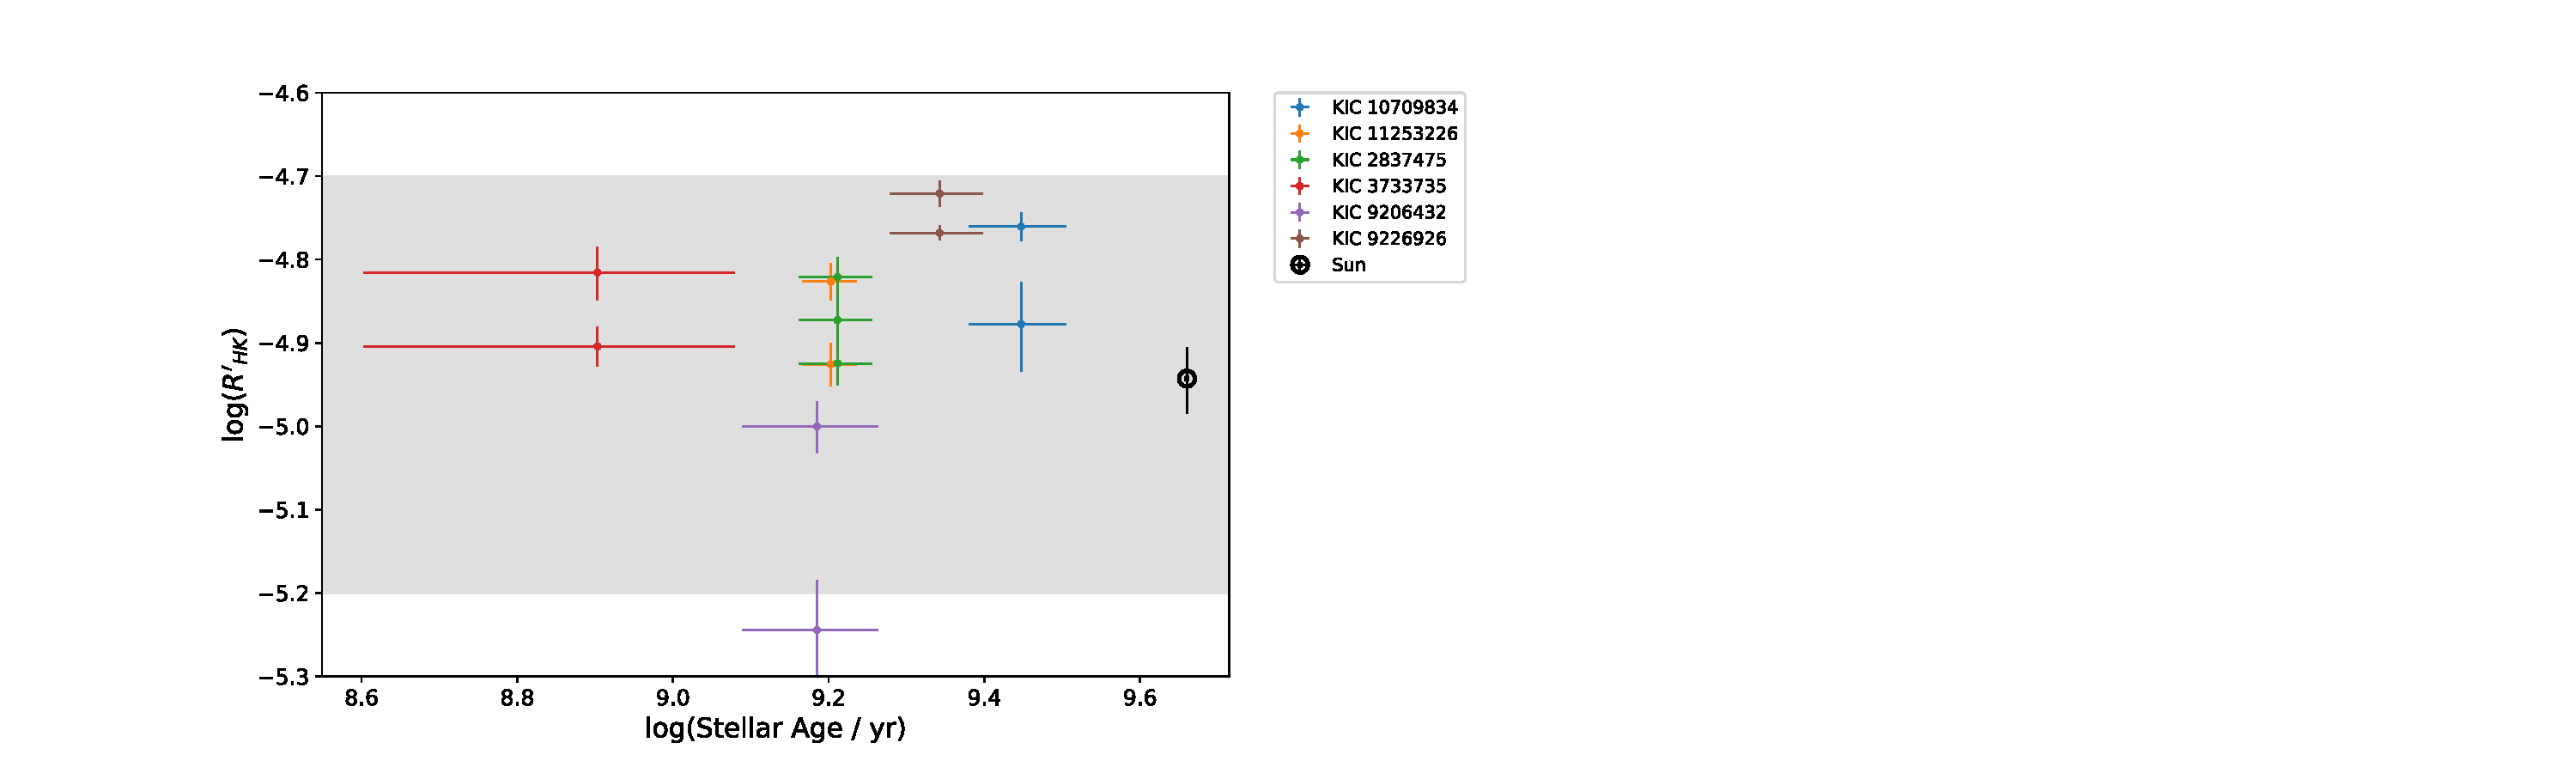
\includegraphics[scale=0.55]{Figures/4-Chromospheric_age/hot_multiple_obs_plot_with_sun.pdf}
    \caption[Plot showing activity over several epochs for stars with $T_{eff} > 6500$ K]{Plot showing \Rprime values calculated using only the H and R channels for multiple observations of stars in our sample with an effective temperature greater than 6500 K. The grey shaded region indicates the range of \Rprime values that our sample occupy.}
    \label{fig:ca_multiple_obs_hot_Fstars}
\end{figure}

\textcolor{red}{Double check the values below - I think I've calculated the correct thing!}

Firstly, considering the sample of stars with $T_{eff} < 6500$ K shown in Figure \ref{fig:ca_multiple_obs}, the plot shows that the typical intrinsic variability of individual stars with multiple observations is in the range 0.03 to 0.2 dex. The mean variability is 0.11 dex with a standard deviation of 0.062. The typical time separation of epochs is between 3 and 6 years, with the original spectra used by \citet{Bruntt_etal_2012} having been collected in 2010.

The total activity spread observed for the 17 mid-F to K stars is ca. 0.35 dex, with a mean \Rprime activity indicator of -5.033 and standard deviation of 0.076, excluding the high-activity outlier star KIC 5774694 discussed in Section \ref{Chp4_results_general_results}. This is significantly larger than the variability observed for individual stars. Therefore, the activity spread seen in Figure \ref{fig:calcium_emission_plot} is unlikely to be caused entirely by intrinsic stellar variability due to potential activity cycles.

Interestingly, the F stars with effective temperatures greater than 6500 K show similar variability properties as the cooler stars; their mean variability is 0.12 with a standard deviation of 0.061. Their variability is shown in a separate plot shown in Figure \ref{fig:ca_multiple_obs_hot_Fstars}. The total variability of the sample is larger with a spread of 0.6 dex, mainly due to one very low activity star.


\subsection{Planet-hosting stars}
From theoretical considerations \citep{Cuntz_etal_2000}, stars with exoplanets in close orbits may experience enhanced stellar activity through star-planet interaction. This effect has been observed for some systems with high-mass exoplanets (see e.g. \citealt{Poppenhaeger_Wolk_2014,Pillitteri_etal_2015}). Two of the stars in the sample have confirmed exoplanets, KIC 9955598 (Kepler-409b) and KIC 10963065 (Kepler-408b). However, Kepler-408b is a small planet with less than five Earth masses in a ca. 2.5-day orbit, and Kepler-409b has a wider orbit with ca. 69-day period \citep{Marcy_etal_2014}. Therefore it is unlikely that those two planets have a significant influence on their host stars' magnetic activity, and star-planet interactions are not expected to play a role in this investigation.

\section{Discussion}
\label{Chp4_discussion}

\subsection{Comparison to existing age-activity relationships}
\label{Chp4_discus_previous_relations}
There have been numerous studies that have calibrated the relationship between the \Rprime indicator and stellar age. In this section, the sample of stars with asteroseismic ages will be compared to these previous relationships.

\begin{figure}
    \centering
    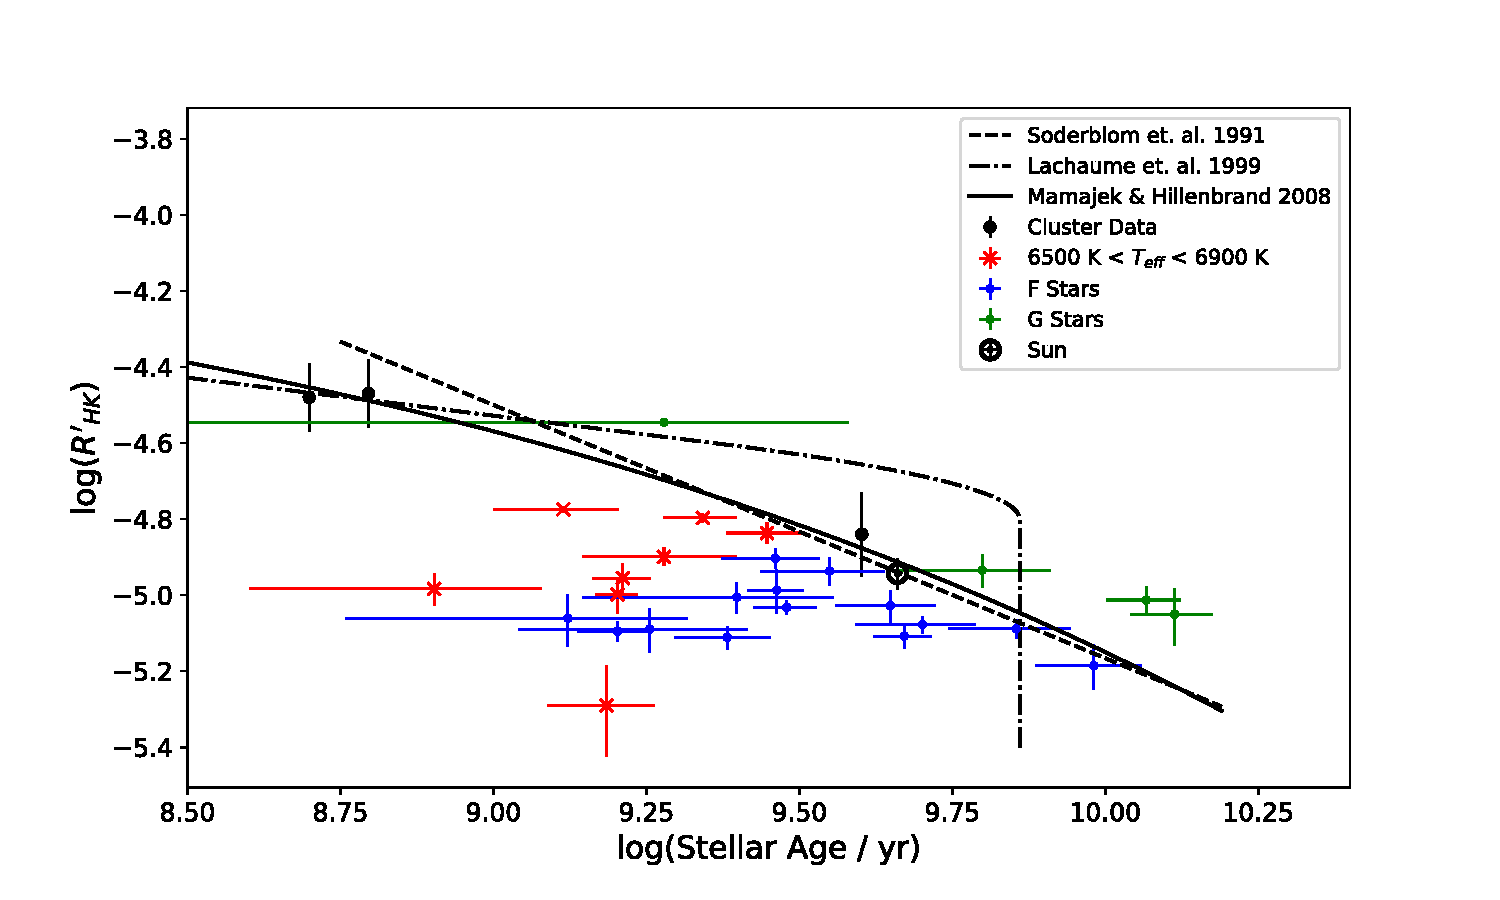
\includegraphics[scale=0.55]{Figures/4-Chromospheric_age/ca_results_3_relationship.pdf}
    \caption[Comparison of sample to previous age-activity relationships]{Plot showing three previously published calibrated relationships between the \Rprime indicator and age \citep{Soderblom_etal_1991,Lachaume_etal_1999,Mamajek_Hillenbrand_2008} alongside the cluster data from \citet{Mamajek_Hillenbrand_2008} and the old sample of stars from this work. The average solar value over several cycles is also shown \citep{Egeland_etal_2017}.}
    \label{fig:comparison_previous_relationships_ca}
\end{figure}

The relationships that we consider are taken from \citet{Soderblom_etal_1991}, \citet{Lachaume_etal_1999} and \citet{Mamajek_Hillenbrand_2008}; these three relationships are shown alongside the sample of old stars analysed in this work in Figure \ref{fig:comparison_previous_relationships_ca}. The first relationship from \citet{Lachaume_etal_1999} is consistent with the two youngest clusters shown in Figure \ref{fig:comparison_previous_relationships_ca}. However, this relationship suggest that the \Rprime indicator does not decay as rapidly as the other two relationships. It is worth noting that they have restricted their sample to B-V $> 0.6$ which ma explain some of the disagreement with the other two relationships. In addition to this, some of their ages are not independent as they have been derived from rotation. The relationship from \citet{Soderblom_etal_1991} shown is the simple power law that they fitted to their data. We see that this relationship has reasonable agreement with the \citet{Mamajek_Hillenbrand_2008} relationship from $\approx$ 1 Gyr. However, it should also be noted that \citet{Soderblom_etal_1991} made an additional fit that included a constraint for constant star formation. This improved the relationship for younger ages but does not affect stars older than the Sun. The third relationship shown in Figure \ref{fig:comparison_previous_relationships_ca} is from \citet{Mamajek_Hillenbrand_2008}. As with the relationship from \citet{Soderblom_etal_1991}, there is good agreement with the cluster data and the solar value. \citet{Mamajek_Hillenbrand_2008} also noted that there was a slight positive trend with colour index. However, for the sample analysed in this work no strong trend with colour index is found.

However, these three relationships do not have good agreement with the sample of old stars considered in this work. The relationships tend to have higher magnetic activity values for a given age than the sample of old stars. This difference could be due to the selection of stars in these studies compared to this work. For example, our sample calculated values for the \Rprime indicator for every star that met our criteria (see Section \ref{Chp4_obs_sample_selection}) and have not excluded stars that do not have visible chromospheric emission. It should also be noted that these studies have used various methods to determine ages for their respective samples including isochronal and cluster ages. However, a common issue is the lack of stars older than a gigayear with reliable and accurate ages. This work has improved on this by considering stars with ages determined by asteroseismology, which has proved to be an accurate age-dating method for old field stars.

Recent work by \citet{Lorenzo_Oliveira_etal_2016} has incorporated mass and metallicity into the age-activity relationship and found good agreement with asteroseismic ages. Therefore, in order to test if the dispersion seen in our sample of stars is due to mass and or metallicity effects we consider variations of the age-mass-metallicity-activity relationship from \citet{Lorenzo_Oliveira_etal_2016} and compare these to the F dwarf stars in our sample.

First, the effect of mass on the age-activity relationship is considered. The top panel in Figure \ref{fig:LO_plot} shows the four oldest clusters from \citet{Mamajek_Hillenbrand_2008} alongside the F stars from our sample. Three variations of the age-activity relationship from \citet{Lorenzo_Oliveira_etal_2016} are also shown - each of these curves assumes solar metallicity and the mass is varied from $1.0 M_{\odot}$ to $1.4 M_{\odot}$ in steps of $0.2 M_{\odot}$. We see that the inclusion of mass into the age-activity relationship changes the shape slightly for stars older than $\approx 1$ Gyr. This can explain some of the dispersion seen in our sample, however, it does not explain the majority of the dispersion.

\begin{figure}
    \centering
    \begin{subfigure}{\textwidth}
        \centering
        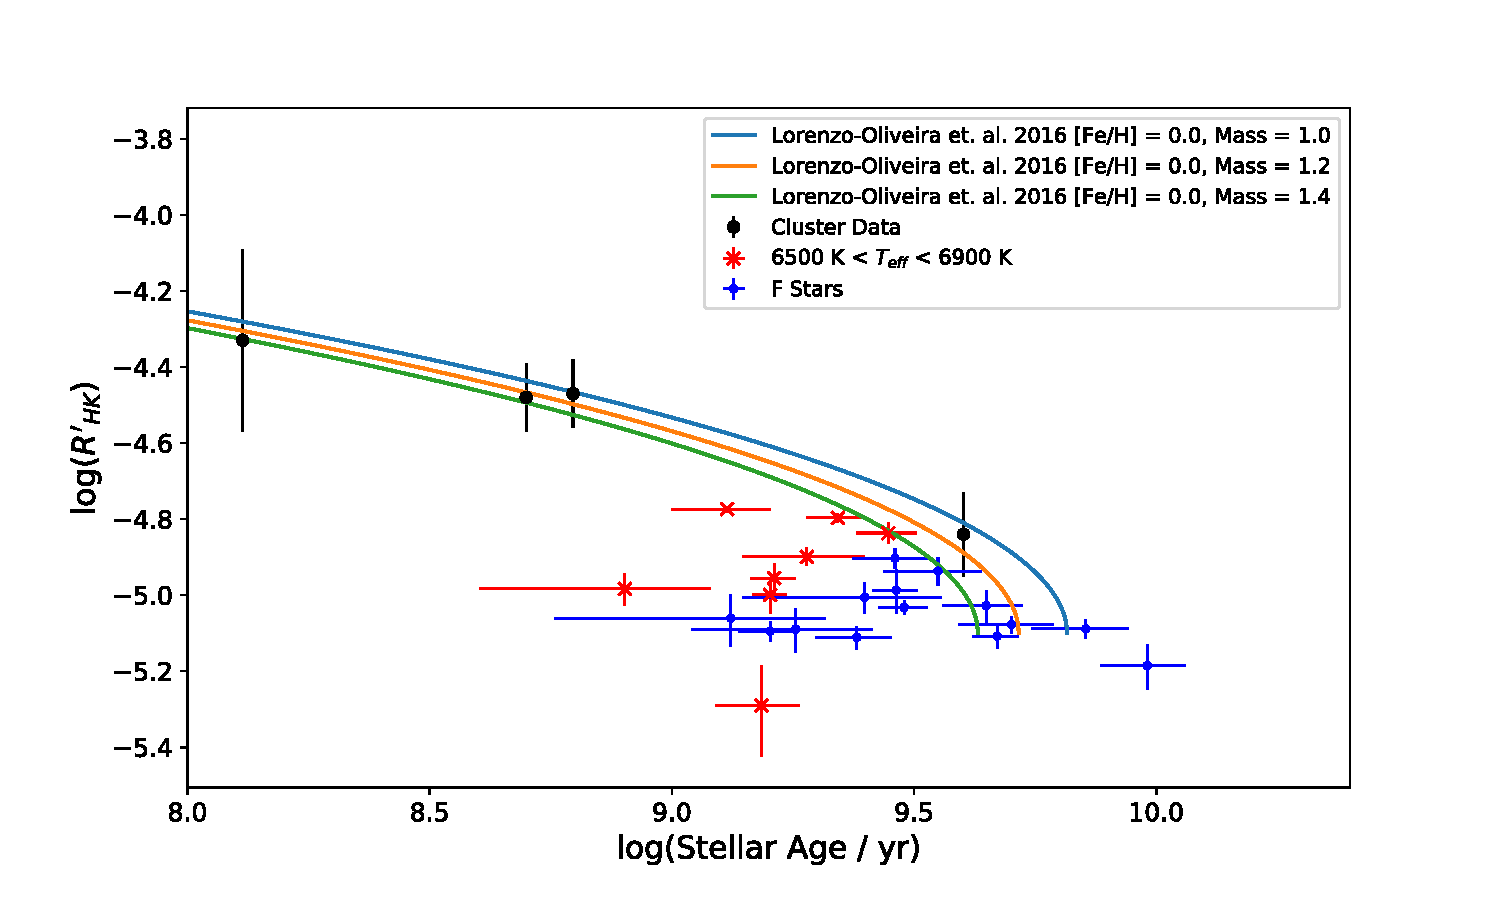
\includegraphics[scale=0.55]{Figures/4-Chromospheric_age/ca_results_LO_mass_w_hotstars.pdf}
        \caption{Effect of mass on age-activity relationship}
    \end{subfigure}
    \begin{subfigure}{\textwidth}
        \centering
        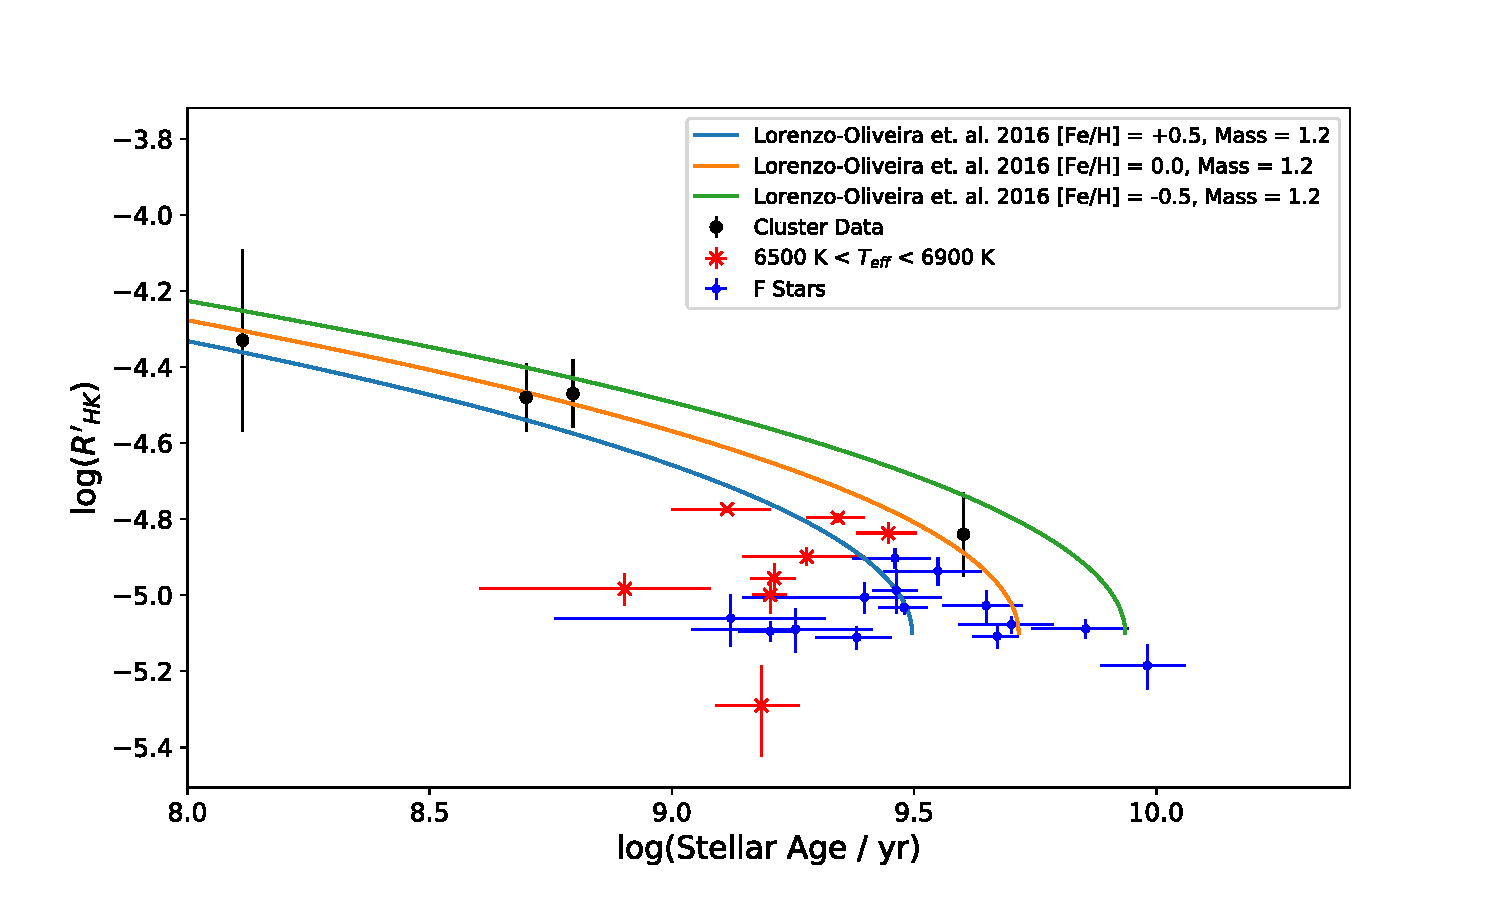
\includegraphics[scale=0.55]{Figures/4-Chromospheric_age/ca_results_LO_metallicity_w_hotstars.pdf}
        \caption{Effect of metallicity on age-activity relationship}
    \end{subfigure}
    \caption[Effect of mass and metallicity on the age-activity relationship]{Plots showing the effect of (a) mass and (b) metallicity on the age-activity relationship using relationship from \citet{Lorenzo_Oliveira_etal_2016}. The oldest clusters from \citet{Mamajek_Hillenbrand_2008} are shown along with the F stars from the sample of stars analysed in this work.}
    \label{fig:LO_plot}
\end{figure}

The effect of metallicity on the age-activity relationship is then considered, this is shown in the bottom panel of Figure \ref{fig:LO_plot}. In this case, the mass is assumed to be $1.2 M_{\odot}$ and three values of metallicity are considered ([Fe/H] = -0.5, 0.0 and +0.5). It is clear to see that metallicity has a greater effect on the age-activity relationship compared to the stellar mass which may be able to explain the dispersion in our data. However, we have a range of stellar masses and metallicities included in our sample, therefore further investigation was warranted.

For our sample of stars, the metallicities are known from \citet{Bruntt_etal_2012} (the original spectroscopy study) and the stellar masses from asteroseismology \citep{Chaplin_etal_2014,Silva_Aguirre_etal_2017}. These parameters were used along with the asteroseismic age to calculate an expected value for the \Rprime indicator from the age-mass-metallicity-activity relationship \citep{Lorenzo_Oliveira_etal_2016}. The measured value of the \Rprime indicator is plotted as a function of the expected value in Figure \ref{fig:Rprime_measured_v_expected}. Figure \ref{fig:Rprime_measured_v_expected} shows that for the majority of our sample, the measured value of the \Rprime indicator is less than the expected value from the age-mass-metallicity-activity relationship. This suggests that there are stars that lie below the predicted age-activity relationship, this is consistent with the X-ray data \citep{Booth_etal_2017} that showed a steepening of the age-activity relationship at ages older than a gigayear.

\begin{figure}
    \centering
    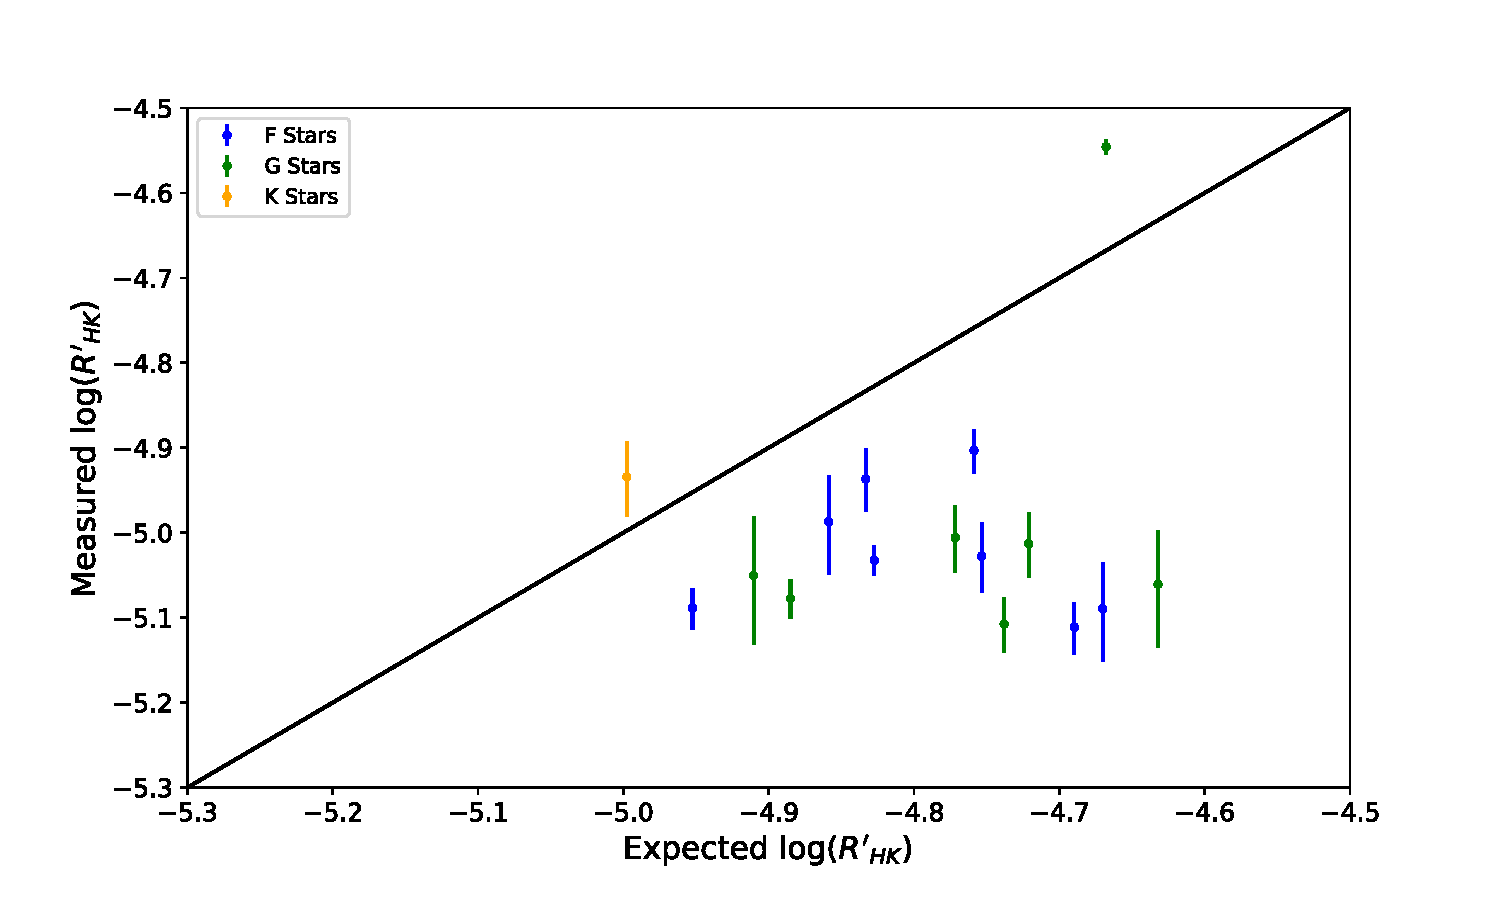
\includegraphics[scale=0.55]{Figures/4-Chromospheric_age/rhk_measured_v_expected.pdf}
    \caption[Measured \Rprime as a function of the expected value including mass and metallicity]{Plot of measured value of the \Rprime indicator from this study as a function of the expected value (as calculated from \citealt{Lorenzo_Oliveira_etal_2016}). The black line shows the 1:1 relationship between the two parameters.}
    \label{fig:Rprime_measured_v_expected}
\end{figure}

One star, KIC 6116048, is missing from the sample in Figure \ref{fig:Rprime_measured_v_expected} due to the combination of its stellar parameters falling outside the range of the \citet{Lorenzo_Oliveira_etal_2016} relationship. This star is shown in Figure \ref{fig:LO_invalid_star} with the age-activity relationship from \citet{Lorenzo_Oliveira_etal_2016} using the relevant stellar parameters. Figure \ref{fig:LO_invalid_star} shows that for this star, when the stellar parameters are entered into the age-mass-metallicity-activity relationship, it results in an age-activity relationship that is not valid for the ages of this star. Therefore, it cannot be used to examine the relationship between the measured value of the \Rprime indicator and the expected value.

\begin{figure}
	\centering
    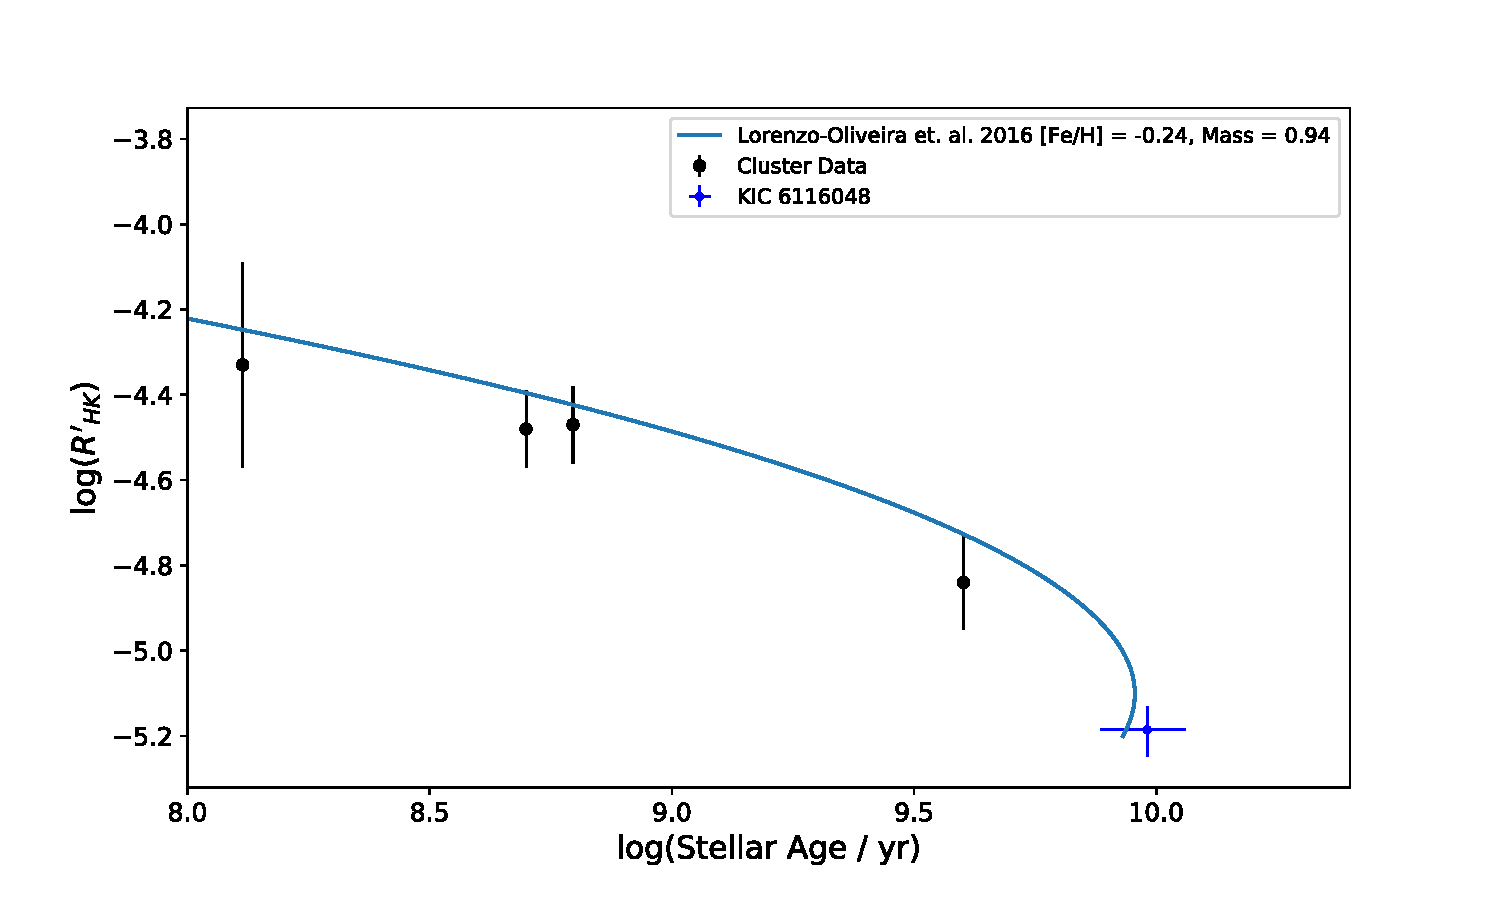
\includegraphics[scale=0.55]{Figures/4-Chromospheric_age/rhk_KIC_6116048.pdf}
    \caption[Plot of age-activity relationship for stellar parameters of KIC 6116048]{Plot showing KIC 6116048 on the age-activity plot. The oldest clusters from \citet{Mamajek_Hillenbrand_2008} are shown along with the relationship from \citet{Lorenzo_Oliveira_etal_2016} using the relevant stellar parameters for the star.}
	\label{fig:LO_invalid_star}
\end{figure}

\subsection{Spin-down in context of observational data}

In recent years, there has been renewed interest into investigating the nature of rotation / magnetic activity - age relationships beyond a gigayear by using ages from asteroseismology \citep{van_Saders_etal_2016,Booth_etal_2017}. \citet{van_Saders_etal_2016} investigated the rotation - age relationship using data from \textit{Kepler} and asteroseismic ages. They found anomalously high rotation rates for older stars and suggested that this was due to weakened magnetic braking. As discussed in the previous Chapter, \citet{Booth_etal_2017} investigated the age-activity relationship by combining X-ray observations with asteroseismic ages. That study found that the X-ray luminosity decays more rapidly for older stars compared to the younger cluster data. One possible explanation for this steepening of the age-activity relationship is due to a change in the activity-rotation relationship.

From the sample of old stars considered in this work, we have determined that mass and metallicity cannot explain all of the dispersion in the age-activity relationship at these older ages. There are stars that lie below the predicted age-activity relationship for a given metallicity and stellar mass (shown in Figure \ref{fig:Rprime_measured_v_expected}). This is consistent with the X-ray data \citep{Booth_etal_2017} as there are inactive stars that lie below the predicted age-activity relationship.

Our sample does not show abnormally high values of the \Rprime indicator that may be associated with weakened magnetic braking at these older ages \citep{van_Saders_etal_2016}. However, we may not expect to see abnormally high values of activity if there is a change in the activity-rotation relationship as suggested by \citet{Booth_etal_2017}. There has also been a recent study into modelling of the stellar wind in time by \citet{OFionnagain_Vidotto_2018}. They presented a way to simultaneously explain the observations of \citet{van_Saders_etal_2016} and \citet{Booth_etal_2017}; the observed decrease in X-ray luminosity is associated with a weaker stellar wind. This weaker stellar wind removes less angular momentum, leading to longer rotation periods as seen in the \textit{Kepler} observations. \citet{OFionnagain_Vidotto_2018} calculated mass-loss rates for a sample of solar-analogues using their 1D polytropic model and found a break in the mass-loss rates at $\approx 2$ Gyr.

\subsection{Chromospheric activity as an age indicator}

In recent years, there has been some debate over the use of chromospheric emission as an age indicator, particularly for stars older than a gigayear. \citet{Pace_2013} presented an L-shaped chromospheric activity versus age diagram and suggested that the use of chromospheric emission as an age indicator is limited to stars younger than $\approx 1.5$ Gyr. However, recent work from \citet{Lorenzo_Oliveira_etal_2016} incorporated mass and metallicity into the age-activity relationship as discussed in Section \ref{Chp4_discus_previous_relations}. In their study, they were also able to reproduce the lack of chromospheric evolution (Figure 2 within) by following the same sample selection procedure as \citet{Pace_2013}. \citet{Lorenzo_Oliveira_etal_2016} found that there was a constant metallicity dispersion along the age axis, which can be understood as an additional source of scatter in the age-activity relationship. They also found that as they considered younger stars, the sample started to become more bias towards higher mass stars.

Our sample of stars shows that even when mass and metallicity are taken into account, there are still stars that lie below the age-activity relationship. Our sample also shows a decrease in the correlation between age and activity for stars older than a gigayear. Therefore, it may be possible that the chromospheric emission decay with age does stop at a relatively young age for the F stars in our sample as suggested by \citet{Pace_2013}. In any case, since the correlation between age and activity decreases for these older stars, we would advise caution in using the \Rprime indicator as an age diagnostic for old main sequence stars.

\subsection{Discrepancy between cluster stars and asteroseismic sample}

\textcolor{red}{TBD - Come back once paper section has been written}

It should be noted that samples taken from asteroseismology have a selection bias towards stars more evolved than the Sun (e.g. \citealt{Metcalfe_etal_2016}). The first selection effect is due to the intrinsic amplitude of solar-like oscillations \citep{Houdek_etal_1999} - they are easier to detect in early-type and more evolved stars. The second is due to the suppression of acoustic mode amplitudes by high magnetic activity \citep{Chaplin_etal_2011_stellar_activity}. This may be of particular importance for the G type stars in our sample as they occupy a much narrower range of activity values than the F stars; possibly indicating that we are lacking more active stars in the sample. Additional data, particularly for younger and more active G-type stars, would confirm if there is any trend in the \Rprime indicator with age for G-type stars.

\section{\texorpdfstring{H-$\alpha$}{H-alpha} Investigation}
\label{Chp4_halpha}
\subsection{Analysis}
An investigation into the use of the \Halpha line (located at 6562.8 \AA) as an age indicator was also conducted as an alternative to the \caII lines. Since the spectra from \citet{Bruntt_etal_2012} cover a wide spectral range, the \Halpha was also available to analyse. The sample selection for the H-$\alpha$ analysis was conducted using the same selection criteria as the \caII data (described in Section \ref{Chp4_obs_sample_selection}); the spectra were also corrected for Doppler shift.

To quantify the chromospheric emission from the \Halpha line, an index analogous to that of the S index is used and is defined by Equation \ref{Eq:h_alpha_index} where $F_{x}$ is the total flux in the relevant channel. There are three channels: the central \Halpha core is measured in a 1.6 \AA \space band centred at 6562.808 \AA \space (C) and two reference channels from 6545.495 - 6556.245 \AA \space (L) and 6575.934 - 6584.684 \AA \space (R) \citep{Gomes_da_Silva_etal_2011}.

\begin{equation}
    Index = \frac{F_{H{\alpha}}}{F_{1}+F_{2}}
    \label{Eq:h_alpha_index}
\end{equation}

A colour corrected index for the \Halpha index was found in \citet{Gomes_da_Silva_etal_2014} known as $I_{H\alpha}$. \citet{Gomes_da_Silva_etal_2014} had a large sample of FGK stars with \textit{HARPS} spectra that were used to calibrate the relationship between the \Halpha index and B-V with the best fitting relationship shown in Equation \ref{Eq:I_H_alpha}. This correction was applied to the \Halpha index calculated for the sample of stars considered in this part of the work.

\begin{equation}
    I_{H\alpha} = H\alpha + 0.019(B-V)^{3} - 0.054(B-V)^{2} + 0.037(B-V)
    \label{Eq:I_H_alpha}
\end{equation}

\subsection{Results and Discussion}
In total, 35 stars were fully analysed and the details of this sample are shown in Appendix REF. Given the location of the \Halpha spectral line, the check for nominal negative flux values in the line core was not necessary thus more stars were analysed in this sample. Four stars have observations from both \esp and \narval spectrographs: KIC 5774694, KIC 8006161, KIC 9139163 and KIC 10454113. For simplicity, only the \narval data is shown in plots for these stars.

\begin{figure}
    \centering
    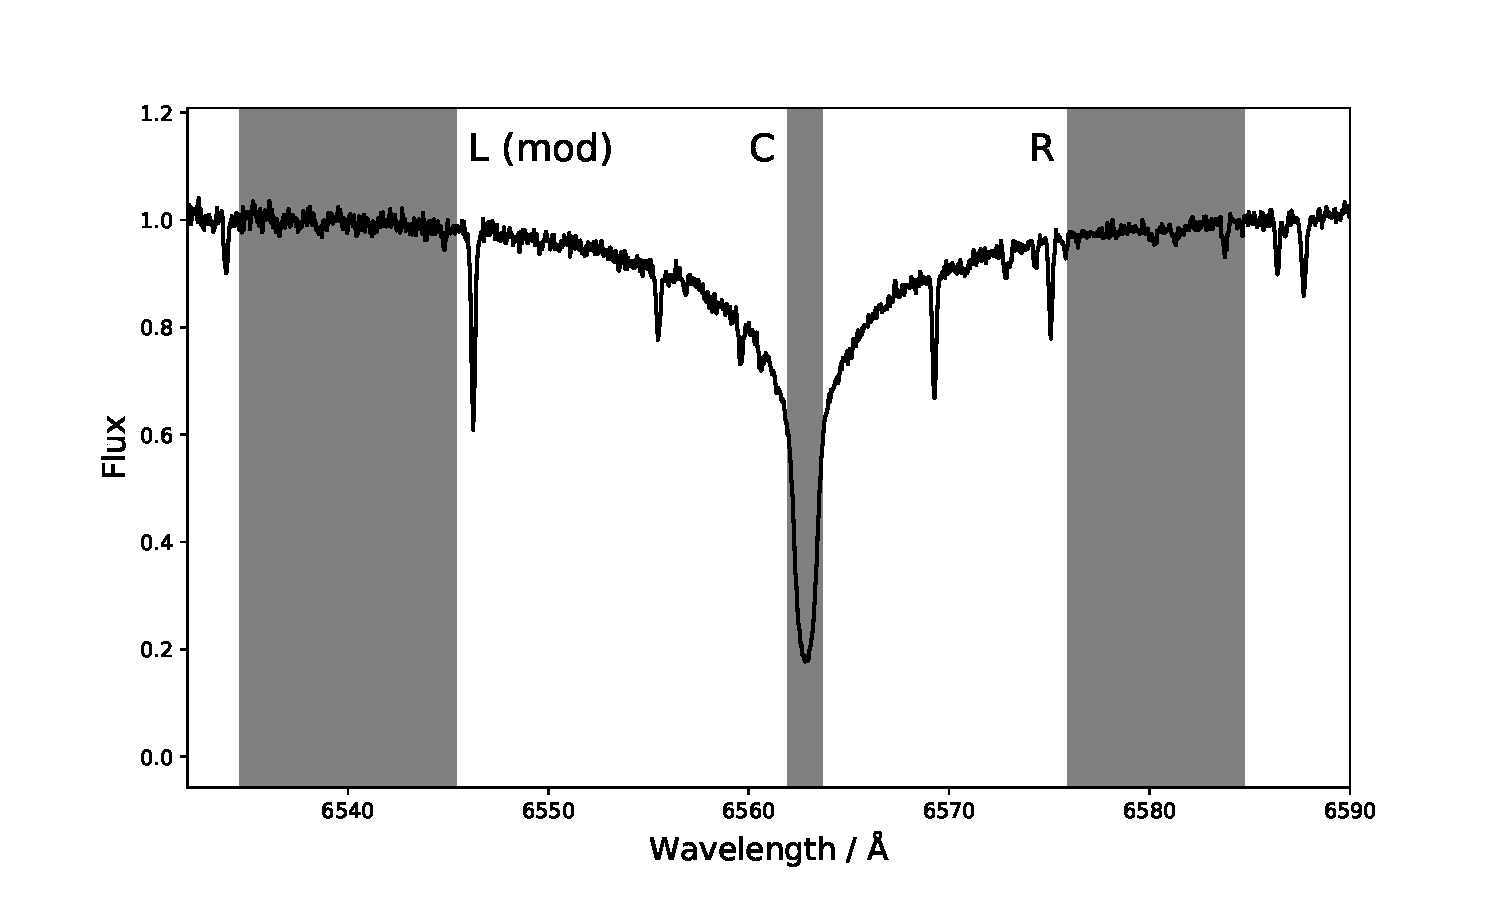
\includegraphics[scale=0.55]{Figures/4-Chromospheric_age/halpha_modified_channels.pdf}
    \caption[Spectra of KIC 9139163 with modified \Halpha channels]{Spectra of KIC 9139163 with modified \Halpha L channel.}
    \label{fig:modified_halpha_channels}
\end{figure}

\begin{figure}
    \centering
    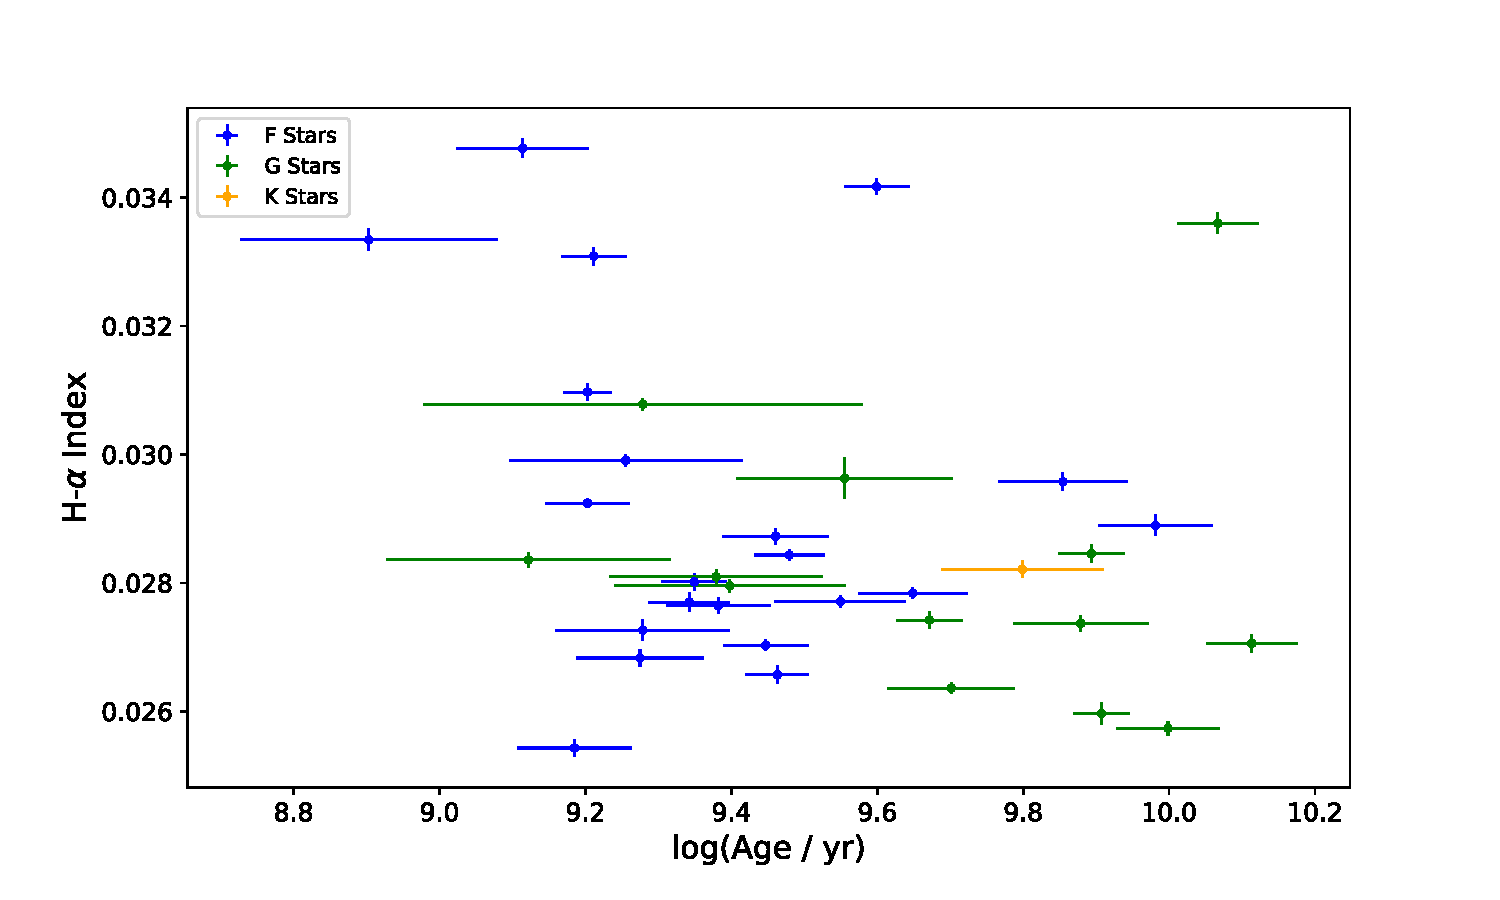
\includegraphics[scale=0.55]{Figures/4-Chromospheric_age/all_data_mod_Halpha_index.pdf}
    \caption[\Halpha index as a function of stellar age]{\Halpha index as a function of stellar age. Spectral types are indicated by different colours.}
    \label{fig:mod_halpha_index_v_age}
\end{figure}

When considering the literature channel values for the \Halpha index, an absorption line located at $\approx$ 6546 \AA \space was found to be located in the L channel. This absorption line varied in strength depending on the spectral type of the star, therefore affecting the value of the \Halpha index calculated. Therefore, the L channel was modified to be centred on 6540 \AA \space (literature channel was centred on 6550.87 \AA), in order to exclude the absorption line as shown in Figure \ref{fig:modified_halpha_channels}. 

Figure \ref{fig:mod_halpha_index_v_age} shows the \Halpha index as a function of age with the \Halpha index calculated using the modified channels shown in Figure \ref{fig:modified_halpha_channels}. However, no conclusions can be drawn from the plot about the nature of the age-activity relationship. Similar to the S index in the calcium emission analysis, the amount of flux in the reference channels will dependent on the mass of the star. Therefore, a colour correction should be applied to the \Halpha index.

In an attempt to apply a colour correction to the \Halpha index, the conversion to $I_{H\alpha}$ \citep{Gomes_da_Silva_etal_2014} was used. However, upon inspection of the $I_{H\alpha}$ versus stellar age plot, the general trend of the activity indicator had not dramatically changed. This prompted an investigation into the \Halpha index and $I_{H\alpha}$ as a function of colour. Figure \ref{fig:halpha_colour_comparison} shows each of these parameters as a function of B-V. The Spearman's rank coefficient was calculated; the coefficients were -0.053 and -0.396 for the \Halpha index and $I_{H\alpha}$, respectively. If the colour correction was successful, one would expect the Spearman's rank coefficient for $I_{H\alpha}$ to be closer to zero than the value for the \Halpha index. Given the values calculated for the sample of stars considered in this work, it is apparent that the conversion to $I_{H\alpha}$ has not removed the mass bias. Additional evidence for this comes from the stars with observations in both the \esp and \narval spectrograph, whose $I_{H\alpha}$ values are not in agreement.

\begin{figure}
    \centering
    \begin{subfigure}{\textwidth}
        \centering
        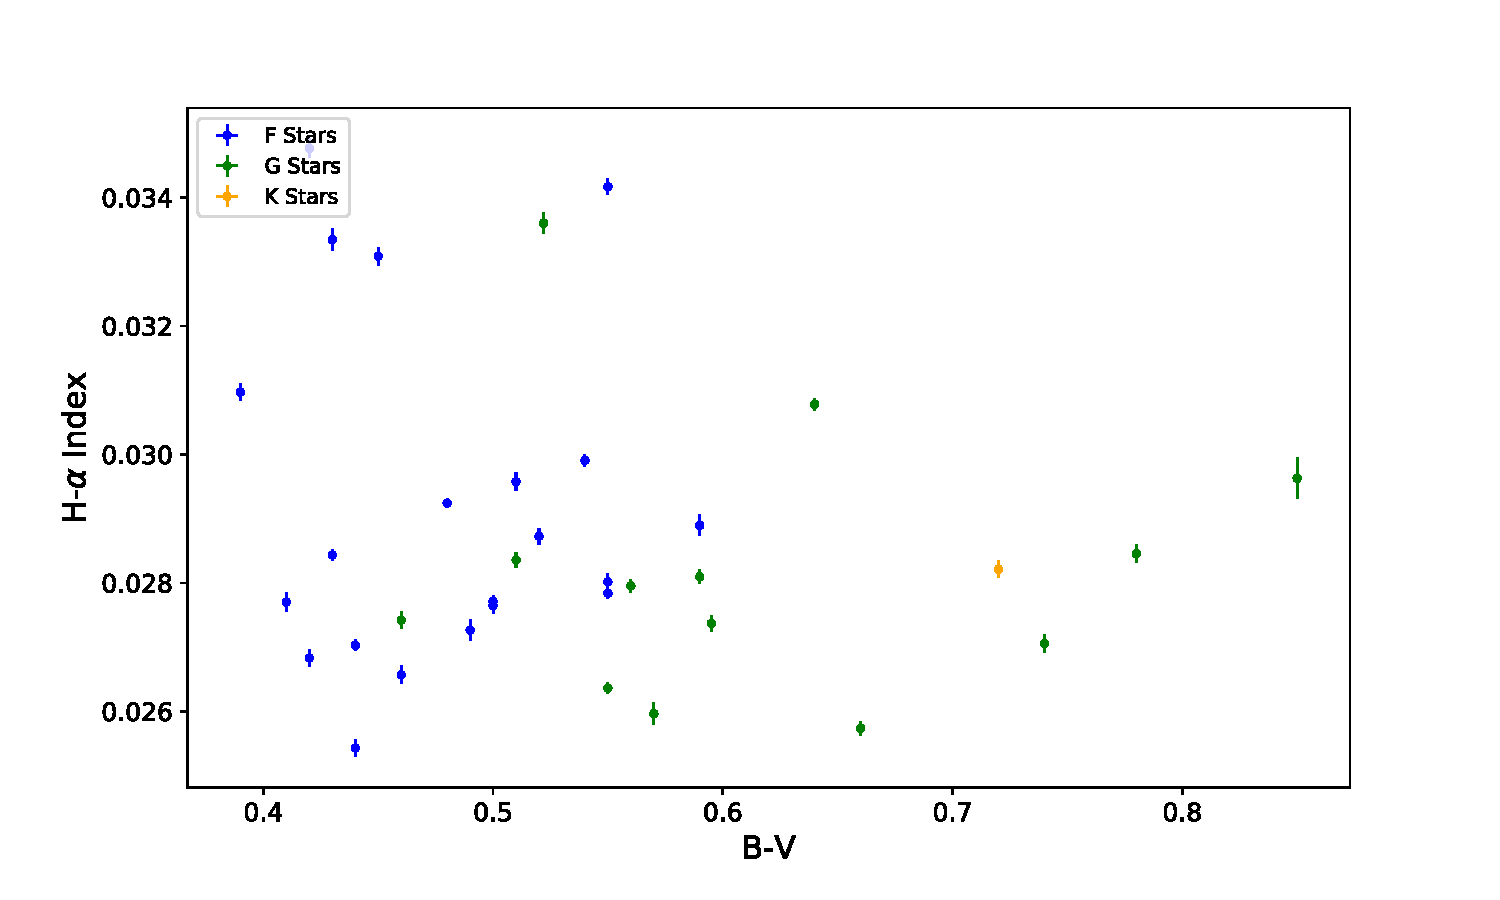
\includegraphics[scale=0.55]{Figures/4-Chromospheric_age/color_comparison_halpha.pdf}
        \caption{\Halpha index as a function of B-V colour}
    \end{subfigure}
    \begin{subfigure}{\textwidth}
        \centering
        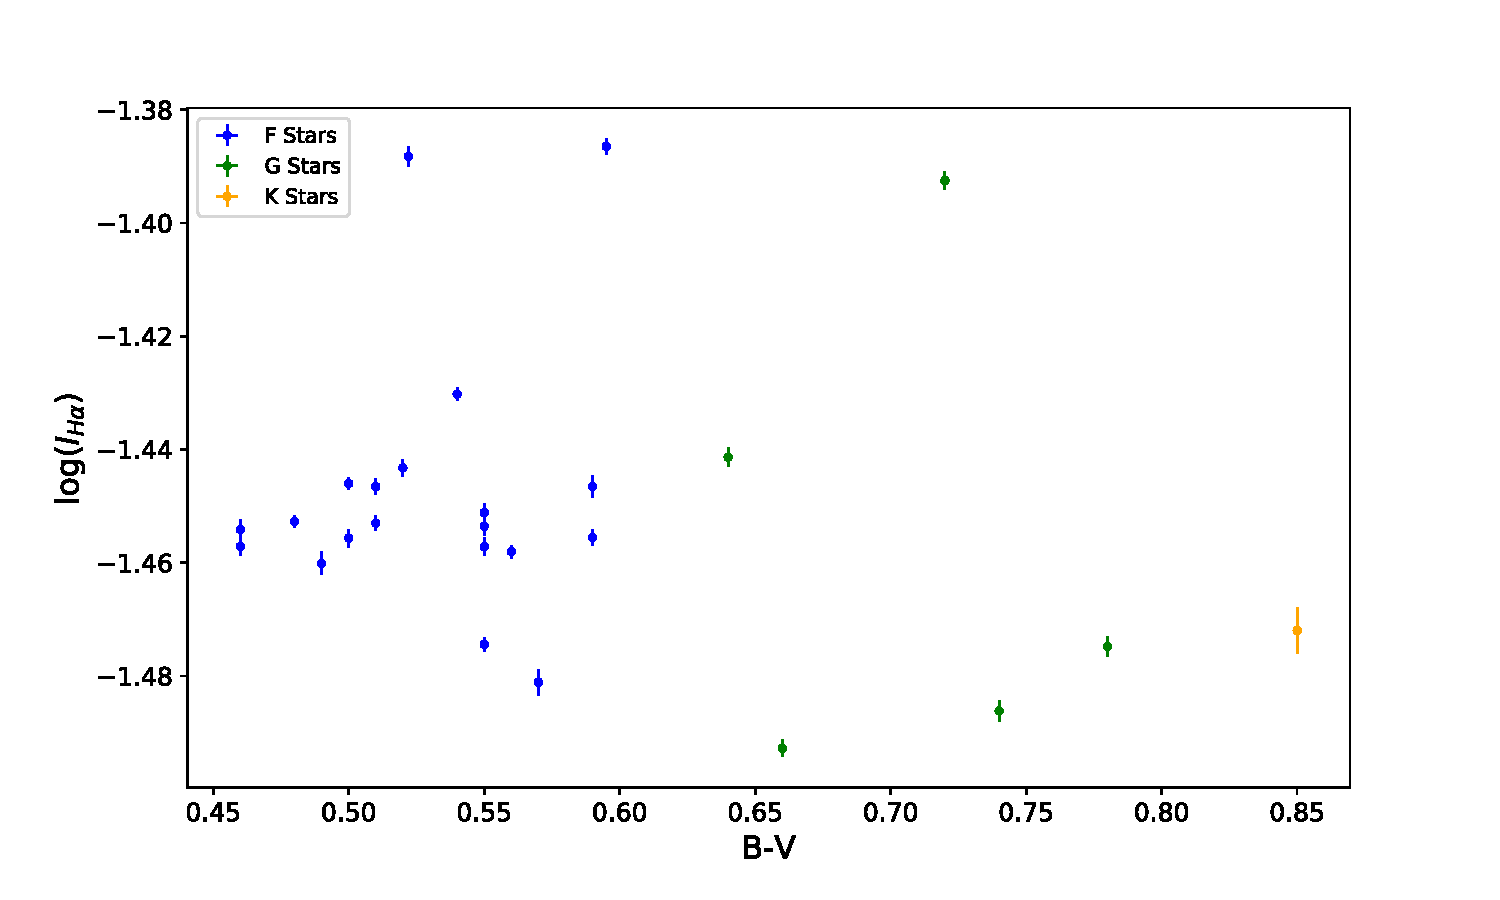
\includegraphics[scale=0.55]{Figures/4-Chromospheric_age/color_comparison_IH.pdf}
        \caption{$I_{H\alpha}$ index as a function of B-V colour}
    \end{subfigure}
    \caption[\Halpha and $I_{H\alpha}$ index as a function of colour]{Plots showing (A) \Halpha index and (B) $I_{H\alpha}$ as a function of B-V colour.}
    \label{fig:halpha_colour_comparison}
\end{figure}

There are several factors that may explain the reason that the conversion to the $I_{H\alpha}$ parameter has been unsuccessful for this sample of stars. However, the most likely reason is that the calculation of the \Halpha index or any index that involves comparison to reference continuum channels is dependent on the spectral resolution and the throughput of the spectrograph used. the calibration to the $I_{H\alpha}$ parameter was based on spectra from \textit{HARPS}. Thus the the relationship was based on values for the \Halpha index calculated from the \textit{HARPS} which will be inherently different than the value calculated from \esp or \narval spectra. In addition to this, the modification of the L channel would have changed the dependence of the \Halpha index as a function of colour as it excluded an absorption line whose strength varied with mass.

In order to use the \Halpha spectral line as an activity indicator for a sample of stars with a wide range of spectral types other methods to include a correct colour correction should be Incorporated. Firstly, a colour correction could be determined for the spectrograph being used; however, this would require a large sample of stars to accurately determine the relationship between the \Halpha index and colour. This would not be possible with the sample considered in this work due to the small number considered and the use of two spectrographs. Alternatively, one could search for calibrator stars with spectra available from both \textit{HARPS} and \esp/\narval. From these calibrator stars, a relationship could be determined between the \Halpha index calculated in each spectrograph. To ensure consistency, the literature channels used in \citet{Gomes_da_Silva_etal_2014} would have to be used to calculate the \Halpha index; this would allow for the conversion to $I_{H\alpha}$ to be used.

\section{Conclusions}
In this work we have presented a sample of 26 cool stars with asteroseismic ages along with calculated values for the \Rprime indicator in an attempt to calibrate the age-activity relationship beyond a gigayear. Relationships were found between the S index calculated in the \narval and \esp spectrographs and \Smw using stars from \citet{Duncan_etal_1991}. This allowed for a conversion to \Smw and the original method by \citet{Noyes_etal_1984} was used to calculate the \Rprime indicator. No strong correlation is found of the \Rprime indicator with age for our sample of stars.

We compared our sample of old stars to previous age-activity relationships and find that for a given age our sample tend to be more inactive than the relationship predicts, particularly for the younger stars in our sample. We also compared our sample to the age-mass-metallicity-activity relationship from \citet{Lorenzo_Oliveira_etal_2016} to see if the inclusion of mass and/or metallicity could explain the dispersion of our sample of old stars. We found that metallicity has a greater effect on the shape of age-activity relationship. We investigated the relationship between the measured value of the \Rprime indicator and the expected value from the \citet{Lorenzo_Oliveira_etal_2016} relationship and found that the majority of our stars lie below the expected age-activity relationship for their metallicity and stellar mass. Given that the majority of our sample follows this trend, this is consistent with X-ray data (\citealt{Booth_etal_2017}, see Chapter \ref{Chapter3}).

Our sample of stars also brings into question the suitability of chromospheric emission as an age indicator for stars older than a gigayear as first suggested by \citet{Pace_2013}. Due to the low correlation between age and activity for our sample of old stars, we would caution the use of the \Rprime indicator as an age diagnostic for ages older than a gigayear.

An additional analysis was performed on the \Halpha spectral line as an alternative to the \caII lines. The \Halpha index was calculated for 26 stars and converted to the $I_{H\alpha}$ parameter \citep{Gomes_da_Silva_etal_2014}. However, upon further investigation into the \Halpha index and $I_{H\alpha}$ as a function of colour, the $I_{H\alpha}$ parameter was unsuccessful in removing the mass bias present in the sample. This is most likely due to the use of a conversion that is calibrated with spectra from a different spectrograph. In order to use the \Halpha spectral line as an activity indicator, a calibration to the \Halpha index calculated in the \textit{HARPS} spectrograph would be needed.






 
% Chapter Template

\chapter{Activity--Rotation--Age Investigation} % Main chapter title

\label{Chapter5} 

\epigraph{\itshape Sometimes the wheel turns slowly, but it turns.}{---Lorne Michaels}

\section{Introduction}

The results presented in Chapters \ref{Chapter3} and \ref{Chapter4} investigated the age-activity relationship through coronal and chromospheric emission. However, the age-activity relationship is a consequence of magnetic braking that removes angular momentum from the star on the main sequence. Thus, the age-activity relationship is inherently link to the rotational evolution. As discussed in Section \ref{Chp2_activity-rotation_lit_review}, this has led to studies on the activity-rotation relationship (see e.g. \citealt{Pizzolato_etal_2003,Wright_etal_2011}). The aim of this study was to collect literature values for the rotation period of the sample of stars considered in the two previous studies and investigate the activity-rotation relationship.

\subsection{Determining rotation periods}
\label{Chp5_Prot_methods}

There are several possible methods to determine the rotation period of a star; since the rotation periods considered in this work were collected from the literature and use various methods, they are summarised here for convenience.

The first method may be the most commonly used to determine the rotation period for a star - photometric variation in light curves due to starspots. As discussed in Section \ref{Chp1_photosphere}, starspots are observed in light curves as periodic variations in the brightness of star as the starspot rotates in and out of view of the observer. To obtain the stellar rotation period, techniques are used to detect periodicities in the light curve. One such technique is the Lomb-Scargle periodogram \citep{Lomb_1976,Scargle_1982}, which uses a Fourier transform to search for periodicities. Typically, a distribution of peaks will appear in the power spectrum and the period with the largest Lomb-Scargle power will correspond to the rotation period. It is a commonly used technique to determine the stellar rotation period (see e.g. \citealt{do_Nascimento_etal_2014,Nielsen_etal_2013}).

Another technique used to determine periodic variations in light curve is the autocorrelation function (ACF); this method determines how correlated the light curve is with itself when offset by a certain time lag. This can be performed for a range of time lags with repeated spot crossings providing peaks in the ACF at time periods associated with the rotation period. An advantage of this method is that the shape of the periodicity in the light curve is not assumed and thus may be more useful in cases where the modulation is not perfectly sinusoidal. This technique is also fairly common in the literature and has been used for large samples of stars from \textit{Kepler} \citep{McQuillan_etal_2014}.

The second method used to determine stellar rotation periods is long term observations of magnetic activity indicators such as the chromospheric emission from the \caII or \Halpha spectral lines and even X-ray luminosity. It is known that these magnetic activity indicators trace active magnetic regions on the surface, thus if an active region crosses the stellar surface multiple times then the rotation period can be determined from the modulation in the magnetic activity indicator. This technique is ideal for stars with more subtle light curve modulation (e.g. slower rotators) as magnetic activity indicators can trace smaller active regions. Examples of this method in the literature include \citet{Boro_Saikia_etal_2016,Robertson_etal_2015_GJ176,DeWarf_etal_2010}.

The third method that can be used to determine the rotation period is from asteroseismology. As discussed in Section \ref{Section:intro_ages}, asteroseismology is a valuable tool for determining fundamental parameters through observations of stellar oscillations. However, one aspect not discussed in the previous section is that any departure from solid body rotation will result in a frequency splitting of non-radial oscillation modes; thus the frequency will also depend on the azimuthal order, m. From helioseismology, the analysis of the frequency splitting due to rotation has provided detail about the interior of the Sun and revealed the presence of the tachocline \citep{Spiegel_Zahn_1992} which is instrumental in stellar dynamo theory . However, in order to obtain rotational splitting from asteroseismology, data sets with timescales on the order of years are required. This is due to the amplitude of the frequency splitting which vary from a few micro-Hertz for more massive or younger stars down to a fraction of a micro-Hertz for less massive or older stars. The frequency splitting of p modes in solar-like oscillators are predominantly determined by the rotational profile in the stellar envelope. There is still some debate in the literature about the accuracy of asteroseismic rotation periods (see e.g. \citealt{Barnes_etal_2016_aspect_gyro}), which will be discussed later in this Chapter.

\section{Data and Method}
\label{Chp5_data_and_method}

The sample of stars considered in this analysis comes from the X-ray luminosity and calcium emission studies conducted in Chapters \ref{Chapter3} and \ref{Chapter4}, respectively. Rotation periods for this sample of stars were searched for in the literature using \textit{VizieR} \citep{Ochsenbein_etal_2000}. In addition to this, literature values for the \Rprime activity indicator were collected for the sample of stars from the X-ray luminosity study. The details of the literature values collected and the relevant references for the sample of stars are shown in Appendix \ref{App_I_activity_rotation}.

Since the sample of stars considered in this work is fairly small, comparison samples from previous activity-rotation studies were also used. To compare the stars with values for the \Rprime indicator, the sample of stars from \citet{Metcalfe_etal_2016} were also plotted. Also, to put the asteroseismic samples into context, data was taken from \citet{Baliunas_etal_1996}. For the X-ray sample, data was taken from \citet{Wright_etal_2011} (W11) to put the sample into context.

As discussed in Section \ref{Chp2_activity-rotation_lit_review}, the activity-rotation relationship is usually calibrated in terms of Rossby number (\Ro). \Ro is defined as the as the rotation period divided by the convective turnover time (\tauc). In this work, \tauc was calculated using the relations from W11 that were derived empirically. By using an empirical method, it assumes that the activity-rotation relationship can be divided into saturated and non-saturated regimes. W11 divided their sample into bins of $B-V$ colour with approximately equal number of stars in each bin. For each mass bin, the activity-rotation relationship was fitted with Equation \ref{Eq:W11_tauc_method_fit_eq} where $(\frac{L_{x}}{L_{BOL}})_{sat}$ and $P_{sat}$ are fitted for each of the mass bins using the $\beta$ value found in W11.

\begin{equation}
    \frac{L_{x}}{L_{BOL}} = 
    \begin{cases}
        C_{B-V}P_{rot}^{\beta} & P_{rot} > P_{sat} \\
        (\frac{L_{x}}{L_{BOL}})_{sat} & P_{rot} < P_{sat}
    \end{cases}
    \label{Eq:W11_tauc_method_fit_eq}
\end{equation}

The fits from each mass bins were used by W11 to determine the colour dependent constant ($C_{B-V}$). The colour dependent constant is defined in Equation \ref{Eq:W11_tauc_method_CBV}, W11 found the colour dependence by setting the scaling constant (C) so that the \tauc value for solar-mass stars matched the values from \citet{Noyes_etal_1984}. This allowed for \tauc to be plotted as a function of colour and/or mass and the best-fitting relationship to be found. It is these best-fitting relationships shown in Equations \ref{Eq:W11_tauc_VK} and \ref{Eq:W11_tauc_mass} that are used to calculate \tauc in this work. In Equation \ref{Eq:W11_tauc_VK}, X is equal to $V-K$ and is valid in the range - $1.1 < V-K < 6.6$.

\begin{equation}
    C_{B-V} = C\tau_{c}^{-\beta}
    \label{Eq:W11_tauc_method_CBV}
\end{equation}

\begin{equation}
    \log \tau_{c} = 
    \begin{cases}
        0.73 + 0.22X & X < 3.5 \\
        -2.16 +1.50X - 0.13X^{2} & X > 3.5
    \end{cases}
    \label{Eq:W11_tauc_VK}
\end{equation}

\begin{equation}
    \log \tau = 1.16 - 1.49\log(M/M_{\odot}) - 0.54\log^{2}(M/M_{\odot})
    \label{Eq:W11_tauc_mass}
\end{equation}

For the majority of the samples considered in this analysis, masses were available and \tauc was calculated using Equation \ref{Eq:W11_tauc_mass}. However, for the sample of stars from \citet{Baliunas_etal_1996}, no masses were available. Therefore, Table 3 from \citet{Pecaut_etal_2012} was used to convert $B-V$ values into $V-K$ values and Equation \ref{Eq:W11_tauc_VK} was used to calculate \tauc. Since the table from \citet{Pecaut_etal_2012} is limited to $B-V < 0.77$, the sample from \citet{Baliunas_etal_1996} was also limited to stars that fell into this range.

\subsection{Consistency of \texorpdfstring{$P_{rot}$}{Prot}}
For a number of stars in the sample, several sources were found for the rotation period in the literature. In this section I will discuss the consistency of the rotation periods found in the literature.

\textit{61 Cyg A}: The rotation period used in this work stems from \citet{Boro_Saikia_etal_2016} and has a value of $35.70$~days. This rotation period was derived from chromospheric activity measurements. Three earlier studies that used the same technique \citep{Vaughan_etal_1981,Hallam_Wolff_1981,Donahue_etal_1996} also have values consistent with the rotation period used in this work.

\textit{61 Cyg B}: The rotation period used in this work comes from \citet{Vaughan_etal_1981} and has a value of $48.0$~days. This value is in agreement with the value found from \citet{Hallam_Wolff_1981}. However, a much shorter rotation period is reported in \citet{Donahue_etal_1996} of $37.84$~days. This is an average rotation period calculated from a number of observations and the range of the rotation periods observed are from $31.78$ to $46.57$~days. Since all of these studies rely on the the measurement of chromospheric emission, the variation in the rotation period may be due to active regions on varying stellar latitudes.

\textit{GJ 176}: This stellar rotation period originates from \citet{Robertson_etal_2015_GJ176} and has a value of $39.46$~days. This rotation period was derived from stellar photometric observations. An additional rotation period was found in \citet{Kiraga_Stepien_2007} that also used photometric variability and found a rotation period consistent with the value used in this work.

\textit{HR 7703}: This stellar rotation period comes from \citet{Ammler_vonEiff_Reiners_2012} and has a minimum value of $17.1$~days. This rotation period is derived from spectral line broadening and the true rotation period larger than this since the stellar inclination is unknown. An erroneous rotation period is reported in \citet{Pizzolato_etal_2003} of $45.0$~days. This rotation period stems from \citet{Saar_etal_1997} and was estimated from the overall \caII emission level.

\textit{KIC 10016239 and KIC 3123191}: The stellar rotation periods used in this work stems from \citet{McQuillan_etal_2014} and have values of $4.89$ and $20.55$~days, respectively. These values are calculated from photometric variation in light curves. \citet{Garcia_etal_2014} also used photometric variation to determine the rotation period for these two stars and found values that are in agreement with the values used in this work.

\textit{KIC 9955598}: The rotation period used in this work originates from \citet{Garcia_etal_2014} and has a value of $34.2$~days. \citet{Garcia_etal_2014} used photometric variation to derived rotation periods. \citet{Paz_Chinchon_etal_2015} also derived a rotation period using photometric variation and found a value for the rotation period of $20.1$~days. However, this was flagged as a lower probability rotation period, therefore the rotation period from \citet{Garcia_etal_2014} was used in this work. 

\textit{Proxima Centauri}: The stellar rotation period comes from \citet{Collins_etal_2017} and has a value of $82.6$~days. This rotation period is calculated from the variability of the \Halpha index. The rotation period is also consistent with the photometric variation as calculated from the Hubble Space telescope \citep{Benedict_etal_1998}.

\textit{KIC 10454113}: The rotation period stems from \citet{McQuillan_etal_2014} and has a value of $14.45$~days. Consistent values for the rotation period for this star are also found in \citet{do_Nascimento_etal_2014} and \citet{Nielsen_etal_2013}.

\textit{KIC 10963065}: The stellar rotation period used in this work originates from \citet{Paz_Chinchon_etal_2015} with a value of $12.96$~days. Similar values for the rotation period were also found in \citet{McQuillan_etal_2013} and \citet{Mazeh_etal_2015}.

\textit{KIC 7206837}: The stellar rotation period comes from \citet{McQuillan_etal_2014} and has a value of $4.07$~days. This value is consistent with the rotation period found in \citet{Nielsen_etal_2013}.

\textit{KIC 9139163}: This star only had one source for the rotation period in the literature \citep{Janes_2017}, however, the rotation period was reported to be $0.61$~days. This is the shortest period found for the sample of stars considered in this work and why it is highlighted here. Unfortunately, no other sources reported a rotation period for this star, therefore it is not possible to determine if this is an erroneous value.

\section{Results}

\subsection{Activity--rotation}
\label{Chp5_results_activity_rotation}

\begin{figure}
    \centering
    \includegraphics[width=0.95\textwidth]{Figures/5-Activity_rotation/Rhk_v_prot.pdf}
    \caption[\Rprime indicator as a function of rotation period]{Plot of the \Rprime indicator as a function of rotation period. Stars from \citet{Metcalfe_etal_2016} and this work are divided into the relevant spectral type.}
    \label{fig:rhk_v_rot}
\end{figure}

From the calcium emission study, eleven stars had rotation periods found in the literature; a further ten stars from the X-ray emission study had literature values for both the rotation period and the \Rprime activity indicator. In addition to this, data from \citet{Metcalfe_etal_2016} were used to compare and compliment the stars from the calcium and X-ray studies. Data from \citet{Baliunas_etal_1996} was also used to place the sample of old, slowly rotating stars with known ages into context.

Figure \ref{fig:rhk_v_rot} shows the \Rprime activity indicator as a function of rotation period for the sample of stars considered in this work. Stars from \citet{Baliunas_etal_1996}, \citet{Metcalfe_etal_2016} and my sample of stars are denoted by triangle, cross and circle symbols, respectively. Furthermore, the \citet{Metcalfe_etal_2016} data and the sample of stars considered in this work are presented by spectral type; F-type stars are shown in blue, G-type stars in green, K-type stars in orange and M-type stars in red. Figure \ref{fig:rhk_v_rot} shows that, as expected, there is a fair amount of scatter in the rotation period for a given activity level. Calculating the Pearson coefficient for the \citet{Baliunas_etal_1996} sample gives a value of $-0.59$, indicating that there is a negative correlation between the two parameters but they are not perfectly anti-correlated. The sample of stars from this work and \citet{Metcalfe_etal_2016} also follow a similar trend and generally agree with the \citet{Baliunas_etal_1996} sample. The exception to this is the M-type stars that have extremely long rotation periods, which is to be expected since they stay on the main sequence for much longer than F, G or K stars and therefore have much longer spin-down timescales.

\begin{figure}
    \centering
    \includegraphics[width=0.95\textwidth]{Figures/5-Activity_rotation/rhk_v_r0.pdf}
    \caption[\Rprime indicator as a function of \Ro]{Plot of the \Rprime indicator as a function of \Ro. The activity-rotation relationship from \citet{Mamajek_Hillenbrand_2008} is shown in black for reference.}
    \label{fig:rhk_v_ro}
\end{figure}

In line with previous activity-rotation studies \citep{Mamajek_Hillenbrand_2008,Metcalfe_etal_2016} we consider the Rossby number instead of rotation period, as shown in Figure \ref{fig:rhk_v_ro}. Note that in order to calculate \Ro for the \citet{Baliunas_etal_1996} sample, the sample was limited to $B-V < 0.77$ as discussed in Section \ref{Chp5_data_and_method}. As expected, the Pearson coefficient value of $-0.66$ shows a stronger negative correlation between the \Rprime indicator and \Ro for the limited \citet{Baliunas_etal_1996} sample of stars. Despite the use of \Ro, there is still a significant spread in \Ro for a given activity level, particularly for low activity levels. Figure \ref{fig:rhk_v_ro} also shows the activity-rotation relationship from \citet{Mamajek_Hillenbrand_2008} (MH08) for comparison, this relationship is valid in the range $-5.0 < \log(R^{'}_{HK}) < -4.3$. The MH08 activity-rotation relationship seems to describe the high activity level for a given Rossby number fairly well. However, there are many lower activity stars that cannot be accurately described by the MH08 relationship. There could be several reasons for this; one possibility is that the MH08 relationship is biased towards more active stars that have detectable light curve modulation due to starspots. Alternatively, as discussed in Section \ref{Chp4_discussion}, the stellar metallicity has an effect on the value of the \Rprime indicator calculated therefore it could be possible that some of this scatter in \Ro for a given activity level is due to metallicity effects.

Twelve stars from the X-ray study \citep{Booth_etal_2017} with determined X-ray luminosities (i.e. not upper limit results) were found to have rotation periods in the literature. This stellar sample is plotted as a function of \Ro alongside the W11 sample of stars as shown in Figure \ref{fig:lx_v_ro}. This plot shows that the sample of old, inactive stars generally lie in the unsaturated regime of the activity-rotation relationship, as expected. However, our sample tends to lie on the lower activity end of the scatter in the activity-rotation relationship. \textcolor{red}{Insert here that more in agreement with beta=-2.7 slope if I put that relationships in Fig 5.3}. The inclusion of the old, inactive sample of stars cannot confirm the potential steepening of the activity-rotation relationship as suggested by \citet{Booth_etal_2017}.

\begin{figure}[!ht]
    \centering
    \includegraphics[width=0.95\textwidth]{Figures/5-Activity_rotation/lx_v_R0.pdf}
    \caption[$L_{x}$ as a function of \Ro]{X-ray luminosity normalised by stellar surface area as a function of \Ro for the sample of stars from the X-ray study with literature rotation periods. The sample from \citet{Wright_etal_2011} is plotted for comparison.}
    \label{fig:lx_v_ro}
\end{figure}

\subsection{Rotation--age}
\label{Chp5_results_rotation_age}
The collection of literature rotation periods for the sample of stars from the X-ray and calcium emission studies also gives the opportunity to investigate the rotation--age relationship. In total, 29 stars from the calcium and X-ray studies have literature rotation periods that are shown in Figure \ref{fig:full_sample_prot_v_age} alongside additional data from \citet{Metcalfe_etal_2016}. Since stellar spin-down is inherently dependent on the mass of the star, the sample was divided into the relevant spectral types for further investigation. 

\begin{figure}[!ht]
    \centering
    \includegraphics[width=0.95\textwidth]{Figures/5-Activity_rotation/prot_v_age.pdf}
    \caption[Rotation period as a function of age for full sample]{Logarithmic plot of rotation period as a function of age for our sample of stars alongside additional data from \citet{Metcalfe_etal_2016}. Stars are displayed by spectral type with the marker denoting the source of the data.}
    \label{fig:full_sample_prot_v_age}
\end{figure}

For each spectral type sample, an ODR was performed on the data using symmetric errors in age and $\log(P_{rot})$ to find the best--fitting relationship between rotation and age. This best--fitting relationship is plotted in black in the following Figures. The \citet{Barnes_2007} gyrochronology relationship was also used for comparison to the sample of old stars. The \citet{Barnes_2007} relationship was calculated for the mean B-V colour of the spectral type sample and plotted in red in the following Figures. It should be noted that the \citet{Barnes_2007} relationship has an age exponent of 0.52, similar to the Skumanich Law. In order to put the sample of old, inactive stars into context, data for clusters were obtained from the literature. These clusters are M67 and Praesepe with rotation periods taken from \citet{Barnes_etal_2016} and \citet{Douglas_etal_2017}, respectively. The ages of M67 and Praesepe are taken to be 4~Gyr and 650~Myr, respectively.

\begin{figure}[!ht]
    \centering
    \includegraphics[width=0.95\textwidth]{Figures/5-Activity_rotation/f_prot_v_age_LR.pdf}
    \caption[Rotation period as a function of age for F-type stars]{Sample of F-type stars with the best--fitting relationship from linear regression shown in green and the \citet{Barnes_2007} gyrochronology relationship for the mean $B-V$ colour of the sample shown in red. Cluster data from M67 and Praesepe are also shown for comparison.}
    \label{fig:f_prot_v_age}
\end{figure}

Figure \ref{fig:f_prot_v_age} shows the F-type stars in the sample along with the cluster data and the \citet{Barnes_2007} relationship. Due to the small errors associated with the rotation periods of the F-type stars and the relatively large errors in age, the ODR found a best-fitting relationship that had large uncertainties in both the gradient and y--intercept. Therefore, for this sample of stars, a linear regression was used. The best fitting relationship from the linear regression is shown in green in Figure \ref{fig:f_prot_v_age}. While the linear regression fit does not take into account the errors associated with the parameters, it gives a much more reasonable best--fitting relationship than the ODR method for this particular sample of stars. The best--fitting relationship for the F stars is shown in Equation \ref{Eq:f_stars_lin_reg} where $t$ is the stellar age in years.

\begin{equation}
    \log(P_{rot}) = (0.91 \pm 0.33)\log(t) -7.69
    \label{Eq:f_stars_lin_reg}
\end{equation}


Figure \ref{fig:f_prot_v_age} shows that the linear regression best--fitting relationship is steeper than the gyrochronology relationship. The gyrochronology relationship seems to be a reasonable fit for the slower rotators in the sample of F-type stars but not the young, fast rotators in the sample. However, the cluster data is in agreement with the \citet{Barnes_2007} relationship and rotate much slower than the best-fitting relationship found in this work would predict.

\begin{figure}[!hbt]
    \centering
    \includegraphics[width=0.95\textwidth]{Figures/5-Activity_rotation/g_prot_v_age.pdf}
    \caption[Rotation period as a function of age for G-type stars]{Sample of G-type stars with the best--fitting relationship from ODR shown in black and the \citet{Barnes_2007} gyrochronology relationship for the mean $B-V$ colour of the sample shown in red. Cluster data from M67 and Praesepe are also shown for comparison.}
    \label{fig:g_prot_v_age}
\end{figure}

Figure \ref{fig:g_prot_v_age} shows the sample of G-type stars along with the cluster data, the \citet{Barnes_2007} relationship and the ODR best-fitting relationship. The best-fitting relationship as found by the ODR method is shown in Equation \ref{Eq:g_stars_ODR}. Similarly to the F-type stars, the gyrochronology relationship agrees with the cluster data and the slower rotators in the sample while the best-fitting relationship does not agree with the cluster data.


\begin{equation}
    \log(P_{rot}) = (0.86 \pm 0.19)\log(t) - (7.00 \pm 1.84)
    \label{Eq:g_stars_ODR}
\end{equation}

\begin{figure}[h!]
    \centering
    \includegraphics[width=0.95\textwidth]{Figures/5-Activity_rotation/k_prot_v_age.pdf}
    \caption[Rotation period as a function of age for K-type stars]{Sample of K-type stars with the \citet{Barnes_2007} gyrochronology relationship for the mean $B-V$ colour of the sample shown in red. Cluster data from M67 and Praesepe are also shown for comparison.}
    \label{fig:k_prot_v_age}
\end{figure}

Figure \ref{fig:k_prot_v_age} shows the sample of K-type stars along with the cluster data and the \citet{Barnes_2007} relationship. Only three stars in the sample are K dwarfs and are sufficiently diverse in age to accurately perform an ODR fit. It is interesting to note that the M67 K-type stars seem to lie below the gyrochronology relationship, this could be due to the difficulty of retrieving longer rotation periods from \textit{K2} data as discussed by \citet{Esselstein_etal_2018}.

\begin{figure}[!ht]
    \centering
    \includegraphics[width=0.95\textwidth]{Figures/5-Activity_rotation/m_prot_v_age.pdf}
    \caption[Rotation period as a function of age for M-type stars]{Sample of M-type stars with the best--fitting relationship from ODR shown in black and the \citet{Barnes_2007} gyrochronology relationship for the mean $B-V$ colour of the sample shown in red. Cluster data from M67 and Praesepe are also shown for comparison.}
    \label{fig:m_prot_v_age}
\end{figure}

Lastly, Figure \ref{fig:m_prot_v_age} shows the M-type stars along with the cluster data from the Praesepe cluster, the \citet{Barnes_2007} relationship and the ODR best-fitting relationship. The best-fitting relationship as found by the ODR method is shown in Equation \ref{Eq:m_stars_ODR}. Note that since the M dwarf stellar sample consists of only three data points, the ODR fit may not be representative of a larger stellar sample. The Praesepe cluster data from \citet{Douglas_etal_2017} was focused on low-mass stars, hence the large number of data points from the cluster in Figure \ref{fig:m_prot_v_age}. The M-type stars in Praesepe also have a large range of rotation periods which is not surprising given that M-type stars take the longest time to converge onto the 'I' sequence to use the terminology from \citet{Barnes_2003}. One may also question the validity of the gyrochronology relationship at these low masses. The \citet{Barnes_2007} relationship was calibrated to a $B-V \approx 1.6$ and the average $B-V$ value of the M-type stars in the sample is $1.65$. Therefore, the gyrochronology may not be accurate in this regime.

\begin{equation}
    \log(P_{rot}) = (0.85 \pm 0.11)\log(t) - (6.41 \pm 1.04)
    \label{Eq:m_stars_ODR}
\end{equation}

\section{Discussion}

\subsection{Rotation--age relationship}
The rotation--age relationships presented in Section \ref{Chp5_results_rotation_age} show that the best--fitting relationships found for the sample of old, inactive stars are not in agreement with the the slower rotators in the sample or the cluster data. However, the \citet{Barnes_2007} relationship is generally in agreement with the cluster data and the slower rotators in the sample. This result could be interpreted in several different ways; firstly, the data could suggest that older stars spin faster than expected and that these older stars have weakened magnetic braking compared to younger stars \citet{van_Saders_etal_2016}. Secondly, there could be a physical change in the nature of the stellar magnetic field that results in a decrease of a variety of starspot properties (e.g. size, decay times, total spot coverage) that could hinder the detection of light curve modulation. Lastly, the rotation periods collected could be biased towards to faster stellar rotators.

The possibility of weakened magnetic braking operating in these older stars is complicated by the presence of slow rotators in the sample. These older and slower rotators that follow the \citet{Barnes_2007} relationship provide evidence that there are stars that rotate as expected for their age and mass. This evidence casts doubt on the interpretation that weakened magnetic braking operates for these stars especially combined with the possibility that there may be biases in the rotation periods collected.

The conclusion that the stellar sample are biased towards faster rotators is a valid concern especially considering that the rotation periods for the majority of the sample stem from light curve modulation caused by starspots. This method in particular is biased towards short rotation periods as it requires a detectable signal caused by fairly large starspots. As stars age and start to spin down, longer timescales are needed to detect variability due to starspots. In addition to this, older stars have fewer and smaller starspots \textcolor{red}{REF?} making measurement of the rotation period via this method even more difficult. To test the hypothesis that older stellar samples are biased towards faster rotators, alternative methods of determining the stellar rotation period are needed. These alternative methods could test if the light curve modulation method is biased towards fast rotators by determining rotation periods independently.

One alternative method is the long-term monitoring of magnetic activity indicators such as the \Rprime indicator. Since the \Rprime indicator traces areas of magnetic activity such as plage \citep{Leighton_1959}, precise calculation of this indicator coupled to observations over several rotation periods can yield the rotation period. This method has been used to determine the rotation for several of the stars considered in this work, particularly for stars that have longer rotation periods \citep{Boro_Saikia_etal_2016,Vaughan_etal_1981,Robertson_etal_2015_GJ191}. This method requires a number of observations over the timescale of several rotation periods to ensure that the \Rprime indicator is sampled sufficiently to accurately determine the rotation period. However, this method also has the advantage of gaining information about the variability of the magnetic activity over a longer timescale.

Another alternative method for determining the stellar rotation period is from asteroseismology. Departures from solid body rotation result in frequency splitting of non-radial oscillation modes and thus the frequency is also dependent on the azimuthal order, m. As discussed in Section \ref{Chp5_Prot_methods}, the frequency splitting of p modes observed in main--sequence stars are largely determined by the rotation profile in the stellar envelope. This is an important aspect of this method, if the stellar rotation period determined from asteroseismology is not the stellar surface rotation, can it be used in gyrochronology relationships? It is this question that makes asteroseismic rotation periods controversial \citep{Barnes_etal_2016_aspect_gyro}. However, some asteroseismology studies find good agreement between the rotation periods determined from asteroseismology and other surface rotation measures \citep{Chaplin_etal_2013,Gizon_etal_2013}. This includes \citet{Davies_etal_2015} who determined the rotation periods for 16 Cyg A \& B from asteroseismology. As an independent validation, they also performed the same analysis on solar data by adding white noise comparable to that found for the stellar data. They find that the asteroseismic rotation for the Sun to be $28.2^{+0.9}_{-1.0}$~days which is consistent with the Carrington rotation period of $27.28$~days. \citet{Davies_etal_2015} suggest that the agreement may be because of an absence of significant differential rotation. They conclude that for 16 Cyg A, the asteroseismic rotation is comparable to surface rotation on the assumption that there is an absence of strong radial differential rotation. Therefore, care must to be taken when considering asteroseismic rotation periods.

The third possible conclusion is that there is a change in the nature of the magnetic activity of these older stars that causes light curve modulation due to starspots to become an inefficient method of determining rotation periods. This was discussed by \citet{van_Saders_etal_2019} as a possible cause for the Rossby number edge present in their rotational distribution for the \textit{Kepler} field. Any decrease in the total stellar spot coverage, star spot size or lifetimes could result in the starspots becoming undetectable in light curve modulation. The steepening of the age--activity relationship \citet{Booth_etal_2017} could also provide observational evidence that there is a change in the magnetic nature of older stars. This will be discussed further in Section \ref{Chp5_discuss_activity_rotation}.

\subsection{Activity-rotation relationship}
\label{Chp5_discuss_activity_rotation}
In Section \ref{Chp5_results_activity_rotation}, the literature rotation periods were used to investigate the activity--rotation relationship for the sample of old, inactive stars. Two activity indicators, calcium and X-ray emission, were considered and here I will discuss the results in the context of recent observational and theoretical studies.

The \Rprime activity indicator was plotted as a function of Rossby number in Figure \ref{fig:rhk_v_ro}. This plot shows that there is significant scatter in the \Rprime--\Ro relationship, this is partly due to mass since this will influence the timescale of the stellar spin-down. However, as discussed in Chapter \ref{Chapter4}, metallicity has a significant effect on the value of the \Rprime activity indicator. This may explain why the activity-rotation from \citet{Mamajek_Hillenbrand_2008} does not fully describe the full sample of old stars or the sample from \citet{Baliunas_etal_1996}.

Figure \ref{fig:lx_v_ro} showed the X-ray luminosity as a function of Rossby number, this clearly showed that the old sample of stars is in general agreement with the previous study by \citet{Wright_etal_2011}. \textcolor{red}{The old sample of stars may be more in favour for a slope of -2.7 for the activity-rotation relationship as \citet{Wright_etal_2011} found for a small, unbiased sample of their data. -- Confirm this once I put slopes in Fig 5.3.} While the old sample of stars considered in this work may give more evidence towards a slight steepening of the activity--rotation relationship, this amount of change in the slope would not be sufficient by itself to warrant the steepening of the X-ray luminosity--age relationship presented in Chapter \ref{Chapter3}. In addition to this, with the report of weakened magnetic braking for older stars \citep{van_Saders_etal_2016}, the slope of the activity--rotation relationship would have to increase further to explain the result presented in Chapter \ref{Chapter3}. 

This result would indicate that an alternative method is responsible for the steepening of the age--activity relationship. Also, if the reported weakened magnetic for older stars \citep{van_Saders_etal_2016} proves to be physical in origin, the physical mechanism at work in these stars must be able to reconcile both the rotational and magnetic activity \citep{Booth_etal_2017} observations. Therefore, it would suggest that the stellar rotational and magnetic evolution no longer go hand in hand at these older ages.

One possible explanation is that there is a change in the magnetic field topology of these older stars. As discussed in Section \ref{Chp4_discus_spindown_context}, this has been suggested for younger stars to explain how they move from the fast rotation branch to the slow rotation branch \citep{Garraffo_etal_2015, Garraffo_etal_2018}; specifically, \citet{Garraffo_etal_2016} suggest that a switch of the stellar magnetic field from a high-order multipole to a low-order one dramatically increases the magnetic braking mediated by the stellar wind. It is possible that for old stars yet another change in magnetic braking takes place, which switches the star to marginal braking again. Another study investigated the stellar wind in simulations, albeit using models with simplifying assumptions; this suggests decreasing mass-loss rates for Sun like stars around ages of ca.\ 2\,Gyr \citep{OFionnagain_Vidotto_2018}.


\section{Conclusions}
In this work, rotation periods were collected for 29 old, inactive stars that were previously studied in Chapters \ref{Chapter3} and \ref{Chapter4}. One of the possible causes for the steepening of the age--activity relationship observed in Chapter \ref{Chapter3} was a change in the activity--rotation relationship for older stars. Therefore, the activity--rotation relationship was investigated using the rotation periods collected from the literature.

The \Rprime--\Ro plot showed significant scatter  for the sample considered that could be a combination of mass and metallicity effects in the \Rprime activity indicator. The activity--rotation relationship from \citet{Mamajek_Hillenbrand_2008} was found to describe the high activity levels well for a given Rossby number. As with the significant scatter seen in the sample, this could be due to mass and/or metallicity effects of the sample used to calibrate the relationship.

When considering the X-ray luminosity as the activity indicator for the activity--rotation relationship, the sample of stars seem to be in agreement with a previous sample of stars \citep{Wright_etal_2011}. \textcolor{red}{However, our sample of stars are more consistent with an exponent value 0f $-2.70$ that was found for a small, unbiased subset of the \citet{Wright_etal_2011} data.} The X-ray luminosity--rotation relationship shows that there is no significant steepening of the relationship as suggested by \citet{Booth_etal_2017}. Therefore, this would suggest that an alternative method is at work to cause the steepening of the age--activity relationship. One possible method is the change in the magnetic topology of the star, this would cause a change in the magnetic braking and explain the steepening of the age--activity relationship.

With the collection of literature rotation periods, the rotation--age relationship was also investigated. This relationship was investigated for each spectral type and found that the best-fitting relationship for the old, inactive sample of stars was inconsistent with the slower rotators in the sample and the cluster data. This evidence could be interpreted in several ways, however, the main conclusion of this investigation is that the biases need to be understood in order to prove whether weakened magnetic braking is physical in origin for these older stars. This can be achieved by considering alternative methods for determining the rotation periods for older stars including  asteroseismology and the monitoring of chromospheric emission from spectral lines such as \caII. Further studies combining age, activity and rotation will improve the sample considered in this work and help shed light on the the possible processes at work in these older stars.



% Chapter Template

\chapter{Conclusions and Outlook} % Main chapter title

\label{Chapter6} % Change X to a consecutive number; for referencing this chapter elsewhere, use \ref{ChapterX}

%----------------------------------------------------------------------------------------
%	SECTION 1
%----------------------------------------------------------------------------------------

\epigraph{\itshape We keep moving forward, opening new doors and doing new things, because we're curious, and curiosity keeps leading us down new paths.}{---Walt Disney}

\section{Conclusions}

Stellar ages gives insight into the timescales of processes at work both within the star (such as the stellar dynamo) or in the environment around the star (e.g. exoplanet dynamics). However, ages are difficult to determine as they cannot be directly calculated from observations of stars. The most successful methods of determining stellar ages (which include stellar isochrones and asteroseismology) are still dependent on stellar models. One potential method of obtaining an estimate for the stellar age is to calibrate an age relationship based on an observable parameter. This is possible for cool stars with an outer convective zone as these stars lose angular momentum via magnetic braking while on the main sequence leading to a decrease in the rotational velocity of the star. This led to the concept of gyrochronology - the study of the rotation period as a function of age. The rotation period is inherently linked to the magnetic activity of the star through the stellar dynamo, therefore an activity-age relationship can also be constructed. With the advancement of asteroseismology allowing ages to be obtained for large samples of field stars, it is now possible to calibrate age relationships using asteroseismic ages. This is the focus of the work presented in this thesis, using stars with asteroseismic ages and observations for magnetic activity indicators to investigate the activity-age relationship. In this thesis I have presented work that has investigated the X-ray luminosity - age relationship, the chromospheric emission - age relationship and finally, the activity-rotation relationship. The results and conclusions for each of these investigations are summarised below.

\subsection{X-ray luminosity - age relationship}

In Chapter \ref{Chapter3}, I presented an investigation into the X-ray luminosity - age relationship for cool stars older than a gigayear. This study presented new X-ray observations of several cool stars along with analysis of archival data to form a sample of 24 stars. Ages for this sample of stars came predominantly from asteroseismology which provide more accurate ages than most other studies were able to provide. Using observations from the \Chandra and \XMM X-ray telescopes, X-ray luminosities were determined for fourteen stars primarily, with spectral modelling for eight of those stars with sufficient photon counts. For ten stars with non-significant detections, upper limits to their X-ray luminosity were calculated.

In order to perform an analysis on the full sample of stars, the mass bias that is present in the X-ray luminosity had to be taken into account. This was achieved by normalising the X-ray luminosity by stellar surface area. An orthogonal distance regression was then used to find the best-fitting relationship between the normalised X-ray luminosity and stellar age for cool stars older than a gigayear. An age-exponent value of $-2.80 \pm 0.72$ was found, representing a steepening of the relationship for cool stars older than a gigayear.

Possible explanations for this steepening of the activity - age relationship include the hypothesis that the rotational spin-down is more rapid than previously thought. However, a recent observational study by \citealt{van_Saders_etal_2016} investigated the rotational evolution of cool stars with asteroseismic ages and found that older stars seemed to be rotating more rapidly than expected. \citet{van_Saders_etal_2016} attribute weakened magnetic braking as the cause for the rapid rotation observed in these stars. The alternative explanation for the steepening of the activity-age relationship is the steepening of the rotation-activity relationship. There is some evidence for such a steepening as seen by \citet{Wright_etal_2011} by considering a small, unbiased sample of their sample. Considering the current evidence towards weakened magnetic braking, the results presented in Chapter \ref{Chapter3} would indicate a steepening of the rotation-activity relationship.

Whatever the underlying reason for the change in the activity - age relationship, our data indicates that there is such a steepening. Further studies incorporating age, activity and rotation will be crucial to understanding what components are responsible for the change seen.

\subsection{Chromospheric emission - age relationship}

In Chapter \ref{Chapter4}, I presented an investigation into the chromospheric emission - age relationship for cool stars older than a gigayear. The main investigation considered how the \Rprime activity indicator evolved over the main sequence lifetime of cool stars. In this part, 26 stars with asteroseismic ages along with calculated values for the \Rprime activity indicator were analysed in an attempt to calibrate the age-activity relationship. Relationships between the S index calculated in the \esp and \narval spectrographs and the \Smw index using stars from \cite{Duncan_etal_1991}. This allowed  for a conversion between to the \Smw and the original method by \citet{Noyes_etal_1984} for the calculation of the \Rprime indicator to be used. No strong correlation of the \Rprime indicator with age was found.

A comparison was made of the sample of old stars with previous age-activity relationships and found that for a given age our sample of stars tended to be more inactive than the relationship predicts, especially for the younger stars in the sample. A comparison was also made between the sample of old stars and the age-mass-metallicity-activity relationship from \citet{Lorenzo_Oliveira_etal_2016} to see if the inclusion of mass and/or metallicity could explain the dispersion of the sample considered in this work. Metallicity was found to have a greater effect on the shape of the age-activity relationship. The relationship between the measured value of the \Rprime indicator and the expected value from the \citet{Lorenzo_Oliveira_etal_2016} relationship was also investigated and it was found that the majority of the sample of old stars lie below the expected age-activity relationship for their mass and metallicity. Given that the majority of the sample follows this trend, this is consistent with the X-ray data presented in Chapter \ref{Chapter3} \citep{Booth_etal_2017}.

The sample of old field stars considered in this research also brings into question the suitability of the \Rprime activity indicator as an age indicator for stars older than a gigayear as previously seen in the literature. Due to the low correlation between age and activity for the sample of old field stars, caution would be advised when considering the \Rprime indicator as an age diagnostic for stars older than a gigayear.

An additional analysis into the \Halpha spectral line was also conducted as an alternative to the \caII lines. The \Halpha index was calculated for 26 stars and converted to the $I_{H\alpha}$ parameter \citep{Gomes_da_Silva_etal_2014}. However, upon further investigation into the \Halpha index and $I_{H\alpha}$ as a function of colour, the $I_{H\alpha}$ parameter was unsuccessful in removing the mass bias present in the sample. This is most likely due to the use of a conversion that is calibrated with spectra from a different spectrograph. In order to use the \Halpha spectral line as an activity indicator, a calibration to the \Halpha index calculated in the \textit{HARPS} spectrograph would be needed.

\subsection{Activity - rotation investigation}

\textcolor{red}{TBD - Once chapter 5 is finished!}

\section{Outlook}

%Currently just thinking of different things, will restructure once all finished
%asteroseismology
The field of asteroseismology is still fairly young, the number of solar-like oscillators detected was only significantly increased by space missions such as Rosat, Kepler and K2 \textcolor(red){INSERT REF FOR MISSIONS}. In order to determine precise ages for asteroseismic targets, detailed modelling of individual oscillation frequencies are required which has been achieved within the past few years \textcolor(red){INSERT REFERENCES!}. However, the sample sizes with asteroseismic ages for age-activity-rotation relationships remain small. The current mission, TESS, is expected to increase the number of stars with detected oscillations by an order of magnitude \textcolor(red){(INSERT Schofield+2019 ref)}. The TESS coverage of the sky is much larger than Kepler/K2
















\begin{appendices}
%Appendix A
\chapter{X-ray spectral modelling plots}
\label{Appendix_Xray_spectra}
%First Figure
\begin{figure}[h]
\begin{subfigure}{\textwidth}
	\centering
	\includegraphics[height = 0.23\paperheight,width=0.9\textwidth]{Figures/3-Xray_age/spec_40eria}
	\caption{40 Eri A}
\end{subfigure}
\begin{subfigure}{\textwidth}
	\centering
	\includegraphics[height = 0.23\paperheight,width=0.9\textwidth]{Figures/3-Xray_age/spec_cd-3710500}
	\caption{CD -3710500}
\end{subfigure}

\caption[X-ray spectra of 40 Eri A and CD -3710500]{X-ray spectra (grouped to 15 counts per bin) and best fit models of two X-ray sources. The top region of each subplot shows the number of counts per second per keV as a function of energy. The bottom region of each subplot shows the sigma value for the best fit model as a function of energy. CD -3710500 was observed with a front-illuminated \textit{Chandra} CCD and therefore only has spectral data above 0.6 keV.}
\label{App_A_40EriA_CD3710500}
\end{figure}

%Second Figure
\begin{figure*}
\begin{subfigure}{\textwidth}
	\centering
	\includegraphics[height = 0.25\paperheight,width=\textwidth]{Figures/3-Xray_age/spec_gj176}
	\caption{GJ 176}
\end{subfigure}
\begin{subfigure}{\textwidth}
	\centering
	\includegraphics[height = 0.25\paperheight,width=\textwidth]{Figures/3-Xray_age/spec_gj191}
	\caption{GJ 191}
\end{subfigure}

\caption[X-ray spectra of GJ 176 and GJ 191]{X-ray spectra (grouped to 15 counts per bin) and best fit models of two X-ray sources. The top region of each subplot shows the number of counts per second per keV as a function of energy. The bottom region of each subplot shows the sigma value for the best fit model as a function of energy.}
\label{App_A_GJ176_GJ191}
\end{figure*}


%Third Figure
\begin{figure*}
\begin{subfigure}{\textwidth}
	\centering
	\includegraphics[height = 0.25\paperheight,width=\textwidth]{Figures/3-Xray_age/spec_hr7703}
	\caption{HR 7703}
\end{subfigure}
\begin{subfigure}{\textwidth}
	\centering
	\includegraphics[height = 0.25\paperheight,width=\textwidth]{Figures/3-Xray_age/spec_kic7529180}
	\caption{KIC 7529180}
\end{subfigure}

\caption[X-ray spectra of HR 7703 and KIC 7529180]{X-ray spectra (grouped to 15 counts per bin) and best fit models of two X-ray sources. The top region of each subplot shows the number of counts per second per keV as a function of energy. The bottom region of each subplot shows the sigma value for the best fit model as a function of energy. Different colours indicate spectra from different detectors which are fitted simultaneously to ensure a more accurate fit.}
\label{App_A_HR7703_KIC7529180}
\end{figure*}

%Fourth Figure
\begin{figure*}
\begin{subfigure}{\textwidth}
	\centering
	\includegraphics[height = 0.25\paperheight,width=\textwidth]{Figures/3-Xray_age/spec_61cyga}
	\caption{61 Cyg A}
\end{subfigure}
\begin{subfigure}{\textwidth}
\centering
\includegraphics[height =        0.25\paperheight,width=\textwidth]{Figures/3-Xray_age/spec_61cygb}
\caption{61 Cyg B}
\end{subfigure}
\par\bigskip

\caption[X-ray spectra of 61 Cyg A and B]{X-ray spectra (grouped to 15 counts per bin) and best fit models for one exemplary observation of 61 Cyg A and B, respectively. These sources were detected to at least three sigma and contained over a hundred counts in the source region. The top region of each subplot shows the number of counts per second per keV as a function of energy. The bottom region of each subplot shows the sigma value for the best fit model as a function of energy. Different colours indicate spectra from different detectors which are fitted simultaneously to ensure a more accurate fit.}
\label{App_A_61Cyg}
\end{figure*}

%Appendix B
\chapter{X-ray luminosity and age results}
\label{App_lx_results}
\begin{landscape}
\begin{table}[htbp]
    \centering
    \begin{minipage}{\linewidth}
		\resizebox{\linewidth}{!}{
			\begin{tabular}{lccccccc}
				Name of Star / White Dwarf & Age / Gyr & log($L_{x}$ / ergs s$^{-1}$) & log($L_{x}/R_{\odot}^{2}$ / ergs s$^{-1}$ $R_{\odot}^{-2}$) & Spectral Type & Age Determination &Age Reference\\
				\hline \hline
				16 Cyg A & $6.67^{0.81}_{0.77}$  & $26.89^{0.10}_{0.10}$ & $26.71^{0.10}_{0.10}$ & G1.5Vb & Asteroseismology & 1  \\
				16 Cyg B & $7.39^{0.89}_{0.91}$ & $<25.85$   & $<25.77$ & G3V & Asteroseismology  & 1  \\
				40 Eri A / 40 Eri B & $3.70^{3.57}_{1.34}$ & $26.81^{0.10}_{0.10}$ & $26.97^{0.10}_{0.10}$ & K0.5V & White Dwarf & 4 \\
				61 Cyg A \footnote{X-ray luminosity adopted from \citet{Robrade_etal_2012}} & $6.00^{1.00}_{1.00}$ & $27.08^{0.23}_{0.23}$ & $27.43^{0.23}_{0.23}$ & K5Ve & Isochrone Fitting & 5 \\
				61 Cyg B \footnote{X-ray luminosity adopted from \citet{Robrade_etal_2012}} & $6.00^{1.00}_{1.00}$ & $26.88^{0.10}_{0.10}$ & $27.33^{0.10}_{0.10}$ & K7V & Isochrone Fitting & 5 \\
				CD -3710500 / L481-60 & $1.77^{0.65}_{0.27}$ & $28.18^{0.10}_{0.10}$ & $28.22^{0.10}_{0.10}$ & G7IV & White Dwarf & 4 \\
				GJ 176 & $2.00^{0.80}_{0.80}$ & $27.03^{0.10}_{0.10}$ & $27.80^{0.10}_{0.10}$ & M2.5V & Member of HR 1614 & 6 \\
				GJ 191 & $11.00^{1.00}_{1.00}$ & $26.41^{0.10}_{0.10}$ & $27.02^{0.10}_{0.10}$ & sdM1.0 & Galactic Halo population & 7 \\
				HR 7703 & $10.00^{2.00}_{2.00}$ & $26.80^{0.10}_{0.10}$ & $27.04^{0.10}_{0.10}$ & K2.5V & Old disk star & 8 \\
				KIC 10016239 & $2.47^{0.67}_{0.61}$ & $27.91^{0.10}_{0.10}$ & $27.71^{0.10}_{0.10}$ & F6IV & Asteroseismology & 2 \\
				KIC 12011630 & $8.48^{1.53}_{1.42}$ & $<30.06$ & $<30.05$ & G1.5V & Asteroseismology & 2 \\
				KIC 3123191 & $4.26^{0.80}_{0.75}$ & $<29.12$ & $<28.84$ & F4.5V & Asteroseismology & 2 \\
				KIC 5309966 & $3.51^{1.23}_{0.42}$ & $<29.44$ & $<29.02$ & F6V & Asteroseismology & 2 \\
				KIC 6116048 & $9.58^{2.16}_{1.90}$ & $<26.89$ & $<26.74$ & F9IV-V & Asteroseismology & 1 \\
				KIC 6603624 & $7.82^{0.94}_{0.86}$ & $<27.08$ & $<26.96$ & G8IV-V & Asteroseismology & 1 \\
				KIC 7529180 & $1.93^{0.35}_{0.30}$ & $28.98^{0.10}_{0.10}$ & $28.66^{0.10}_{0.10}$ & F5IV-V & Asteroseismology & 2 \\
				KIC 8292840 & $3.85^{0.81}_{0.75}$ & $<28.14$ & $<27.88$ & F7V & Asteroseismology & 3 \\
				KIC 9025370 & $6.55^{1.26}_{1.13}$ & $<27.24$ & $<27.23$ & F8 & Asteroseismology & 1 \\
				KIC 9410862 & $6.93^{1.49}_{1.33}$ & $<27.98$ & $<27.86$ & F7V & Asteroseismology & 1 \\
				KIC 9955598 & $6.98^{0.40}_{0.50}$ & $26.90^{0.10}_{0.10}$ & $27.01^{0.10}_{0.10}$ & K0V & Asteroseismology & 3 \\
				NLTT 7887 / NLTT 7890 & $4.97^{8.80}_{3.00}$ & $<26.92$ & $<27.13$ & K2 & White Dwarf & 4 \\
				Proxima Centauri  \footnote{X-ray luminosity taken from \citet{Fuhrmeister_etal_2011}} & $6.13^{0.55}_{0.55}$ & $26.69^{0.10}_{0.10}$ & $28.23^{0.10}_{0.10}$ & M5.5Ve & Asteroseismology & 9 \\
				Alpha Centauri B \footnote{X-ray luminosity adopted from \citet{Robrade_etal_2012}} & $6.13^{0.55}_{0.55}$ & $27.06^{0.36}_{0.36}$ & $27.19^{0.36}_{0.36}$ & K1V & Asteroseismology & 9 \\
				Sun \footnote{X-ray luminosity adapted from model values given in \citet{Peres_etal_2000}} & $4.57^{0.02}_{0.02}$ & $26.77^{0.72}_{0.72}$ & $26.77^{0.72}_{0.72}$ & G2V & Isotopic Dating & 10 \\
				\hline  
     
			\end{tabular}}
			\caption[Full X-ray luminosity results]{\begin{footnotesize}		
		\noindent \textbf{References}: (1) \citet{Silva_Aguirre_etal_2017}; (2) this work, age recalculated with BASTA algorithm \citep{Silva_Aguirre_etal_2015} using values from \citet{Chaplin_etal_2014} and  \citet{Buchhave_Latham_2015}; (3) \citet{Silva_Aguirre_etal_2015}; (4) this work, see Section \ref{Section_sample_selection}; (5) \citet{Kervella_etal_2008}; (6) \citet{Feltzing_Holmberg_2000}; (7) \citet{Anglada_Escude_etal_2014}; (8) \citet{DeWarf_etal_2010}; (9) \citet{Miglio_Montalban_2005}; (10) \citet{Bahcall_etal_1995}
		
        \end{footnotesize}}
        
	\end{minipage}
\end{table}
\end{landscape}

%Appendix C
\chapter{Stellar properties of X-ray sample}
\label{App_Xray_sample_stellar_properties}

\begin{table}[h!]
\centering
\resizebox{0.95\textwidth}{!}{
	\begin{tabular}[h]{l l l l l l}
		\hline \hline
		Name of Star / White Dwarf & Radius / $R_{\odot}$ & $T_{eff}$ / K & $V_{mag}$ & Distance / pc & References\\
		\hline 
		16 Cyg A & 1.22 & 5825 & 5.95 & 21.29 & 1,6,8,10 \\
		16 Cyg B & 1.10 & 5720 & 6.20 & 21.22 & 1,6,8,10  \\
		40 Eri A / 40 Eri B & 0.83  & 5225 & 4.43 & 4.98 & 5,6,8,9 \\
		61 Cyg A & 0.67 & 4450 & 5.21 & 3.49 & 4,6,8,9 \\
		61 Cyg B & 0.60 & 4050 & 6.03 & 3.50 & 4,6,8,9 \\
		CD -3710500 / L481-60 & 0.96 & 5530 & 6.01 & 15.25 & 5,6,8,10 \\
		GJ 176 & 0.41 & 3475 & 9.95 & 9.27 & 5,6,8,9 \\
		GJ 191  & 0.49 & 3680 & 8.85 & 3.91 & 5,6,8,9 \\
		HR 7703 & 0.77 & 4940 & 5.32 & 6.02 & 5,6,8,9 \\
		KIC 10016239 & 1.26 & 6482 & 9.81 & 175.93 & 3,7,8,10 \\
		KIC 12011630 & 1.01 & 5817 & 10.27 & 114.40 & 3,7,8,11 \\
		KIC 3123191 & 1.37 & 6568 & 9.90 & 167.67 & 3,7,8,10 \\
		KIC 5309966 & 1.62 & 6356 & 10.62 & 288.60 & 3,7,8,10 \\
		KIC 6116048 & 1.19 & 6072 & 8.47 & 75.15 & 1,7,8,10 \\
		KIC 6603624 & 1.15 & 5612 & 9.19 & 83.56 & 1,7,8,10 \\
		KIC 7529180 & 1.45 & 6682 & 8.49 & 108.53 & 3,7,8,10 \\
		KIC 8292840 & 1.35 & 6239 & 10.51 & 250.69 & 2,2,8,9 \\
		KIC 9025370 & 1.00 & 5659 & 8.95 & 87.42 & 1,7,8,10 \\
		KIC 9410862 & 1.16 & 6230 & 10.78 & 202.27 & 1,7,8,10 \\
		KIC 9955598 & 0.88 & 5434 & 9.64 & 69.39 & 2,7,8,10 \\
		NLTT 7887 / NLTT 7890 & 0.78 & 5040 & 9.84 & 41.16 & 5,6,8,10 \\
		Proxima Centauri & 0.17 & 2925 & 11.13 & 1.30 & 5,6,8,9 \\
		Alpha Centauri B & 0.86 & 5316 & 1.33 & 1.35 & 12,12,8,12 \\
		Sun  & 1.00 & 5777 & -26.74 & 1 AU & 13 \\    
		\hline 
	\end{tabular}}
	
	\caption[Stellar properties of X-ray luminosity sample]{\begin{footnotesize}		
	\noindent
	\textbf{References}: (1) \citet{Silva_Aguirre_etal_2017}; (2) \citet{Silva_Aguirre_etal_2015}; (3) this work, radius recalculated with BASTA algorithm \citep{Silva_Aguirre_etal_2015} using values from \citet{Chaplin_etal_2014} and  \citet{Buchhave_Latham_2015}; (4) \citet{Kervella_etal_2008}; (5) Radius calculated from $T_{eff}$ and absolute brightness; (6) $T_{eff}$ estimated from Spectral Type using Table 5 from \citet{Pecaut_Mamajek_2013}; (7) \citet{Chaplin_etal_2014}
	(8) $V_{mag}$ from SIMBAD; (9) Parallax from SIMBAD; (10) Parallax from \textit{Gaia} DR1 \citep{Gaia_Collaboration_2016_DR1}; (11) Distance from Barnes-Evans method (see Section \ref{Section_Xray_distances_and_spectype} for details); (12) \citet{DeWarf_etal_2010}
	\end{footnotesize}}
\end{table}
\clearpage

%Appendix D
\chapter{Stars used to calibrate to \texorpdfstring{\Smw}{Smw} index}
\label{App_calibrator_stars_Smw}

%ESPADONS TABLE
\begin{longtable}{llccc}
\caption[\esp calibrator stars for \Smw relationship]{List of calibrator stars \citep{Duncan_etal_1991} used to calibrate the relationship between the S index calculated from \esp spectra and \Smw. Spectral types and $B-V$ taken from SIMBAD \citep{Wenger_etal_2000}.}\\

\hline
Star Name         & Spectral Type & $B-V$  & Average \Smw & \esp S Index \\
\hline
\endfirsthead

\hline
Star Name         & Spectral Type & $B-V$  & Average \Smw & \esp S Index \\
\hline
\endhead

\hline
\endfoot
 
\hline
\endlastfoot

\renewcommand{\arraystretch}{1.2}

Cl Melotte 22 1613 & G0            & 0.54 & 0.3077 & $0.0119^{0.0006}_{0.0006}$\\
HD 124897          & K1.5III       & 1.23 & 0.1441 & $0.0075^{0.0001}_{0.0001}$\\
HD 144579          & G8V           & 0.73 & 0.1628 & $0.0081^{0.0005}_{0.0005}$\\
HD 159181          & G2Ib-IIa      & 0.98 & 0.3019 & $0.0167^{0.0002}_{0.0002}$\\
HD 171635          & F7Ib          & 0.62 & 0.0499 & $0.0017^{0.00002}_{0.00002}$\\
HD 177241          & G9IIIb        & 1.00 & 0.1057 & $0.0053^{0.0001}_{0.0001}$\\
HD 179958          & G2V           & 0.65 & 0.1571 & $0.0068^{0.0002}_{0.0002}$\\
HD 182572          & G7IV          & 0.77 & 0.1543 & $0.0071^{0.0002}_{0.0002}$\\
HD 185351          & G8.5IIIb      & 0.94 & 0.1946 & $0.0116^{0.0001}_{0.0001}$\\
HD 186408          & G1.5Vb        & 0.64 & 0.1476 & $0.0071^{0.0001}_{0.0001}$\\
HD 186427          & G3V           & 0.66 & 0.1450 & $0.0073^{0.0003}_{0.0003}$\\
HD 187691          & F8V           & 0.56 & 0.1479 & $0.0059^{0.0004}_{0.0004}$\\
HD 192876          & G3Ib          & 1.07 & 0.2510 & $0.0129^{0.0001}_{0.0001}$\\
HD 194093          & F8Ib          & 0.67 & 0.0564 & $0.0039^{0.0005}_{0.0005}$\\
HD 204867          & G0Ib          & 0.82 & 0.1617 & $0.0074^{0.0001}_{0.0001}$\\
HD 206859          & G5Ib          & 1.17 & 0.2041 & $0.0140^{0.0002}_{0.0002}$\\
HD 209750          & G2Ib          & 0.96 & 0.2081 & $0.0117^{0.0001}_{0.0001}$\\
HD 217014          & G2IV          & 0.70 & 0.1548 & $0.0068^{0.0002}_{0.0002}$\\
HD 26630           & G0Ib          & 0.96 & 0.3623 & $0.0148^{0.0001}_{0.0001}$\\
HD 31910           & G1Ib          & 0.93 & 0.2659 & $0.0124^{0.0001}_{0.0001}$\\
HD 3795            & K0V           & 0.70 & 0.1587 & $0.0069^{0.0001}_{0.0001}$\\
HD 39587           & G0V           & 0.60 & 0.3067 & $0.0173^{0.0001}_{0.0001}$\\
HD 7924            & K0.5V         & 0.85 & 0.2221 & $0.0102^{0.0001}_{0.0001}$\\
HD 89449           & F6IV-V        & 0.44 & 0.1781 & $0.0078^{0.0001}_{0.0001}$\\
HD 98736		   & G5			   & 0.84 & 0.1940 & $0.0096^{0.0001}_{0.0001}$\\
Parenago 1394	   & F8			   & 0.48 & 0.2635 & $0.0141^{0.0003}_{0.0003}$\\
\hline
\end{longtable}

%NARVAL TABLE
\begin{longtable}{llccc}
\caption[\narval calibrator stars for \Smw relationship]{List of calibrator stars \citep{Duncan_etal_1991} used to calibrate the relationship between the S index calculated from \narval spectra and \Smw. Spectral types and $B-V$ taken from SIMBAD \citep{Wenger_etal_2000}.}\\

\hline
Star Name         & Spectral Type & $B-V$  & Average \Smw & \narval S Index \\
\hline
\endfirsthead

\hline
Star Name         & Spectral Type & $B-V$  & Average \Smw & \narval S Index \\
\hline
\endhead

\hline
\endfoot
 
\hline
\endlastfoot

\renewcommand{\arraystretch}{1.2}

Cl Melotte 111 58 & F7V           & 0.45 & 0.2903        & $0.0159^{0.0002}_{0.0002}$ \\
Cl Melotte 111 97 & F9V           & 0.55 & 0.2978        & $0.0169^{0.0002}_{0.0002}$ \\
HD 103095         & K1V           & 0.75 & 0.1828        & $0.0093^{0.0001}_{0.0001}$ \\
HD 109358         & G0V           & 0.61 & 0.1774        & $0.0074^{0.0001}_{0.0001}$ \\
HD 114710         & F9.5V         & 0.59 & 0.2000        & $0.0087^{0.0001}_{0.0001}$ \\
HD 126660         & F7V           & 0.51 & 0.2500        & $0.0124^{0.0001}_{0.0001}$ \\
HD 145675         & K0V           & 0.90 & 0.1514        & $0.0074^{0.0001}_{0.0001}$ \\
HD 148816         & F7V           & 0.53 & 0.1621        & $0.0068^{0.0001}_{0.0001}$ \\
HD 150680         & G0IV          & 0.63 & 0.1354        & $0.0064^{0.0001}_{0.0001}$ \\
HD 154345         & G8V           & 0.76 & 0.1927        & $0.0084^{0.0001}_{0.0001}$ \\
HD 154417         & F8.5IV-V      & 0.58 & 0.2706        & $0.0130^{0.0001}_{0.0001}$ \\
HD 161797         & G5IV          & 0.75 & 0.1359        & $0.0076^{0.0002}_{0.0002}$ \\
HD 162003         & F5IV-V        & 0.44 & 0.1669        & $0.0075^{0.0001}_{0.0001}$ \\
HD 164922         & G9V           & 0.80 & 0.1598        & $0.0075^{0.0001}_{0.0001}$ \\
HD 16895          & F8V           & 0.51 & 0.1587        & $0.0066^{0.0001}_{0.0001}$ \\
HD 171635         & F7Ib          & 0.62 & 0.0499        & $0.0018^{0.0001}_{0.0001}$ \\
HD 176377         & G1V           & 0.59 & 0.1772        & $0.0089^{0.0001}_{0.0001}$ \\
HD 177830         & K0+M4V        & 1.09 & 0.1233        & $0.0059^{0.0001}_{0.0001}$ \\
HD 183650         & G5            & 0.71 & 0.1237        & $0.0055^{0.0002}_{0.0002}$ \\
HD 184499         & G0V           & 0.58 & 0.1449        & $0.0070^{0.0001}_{0.0001}$ \\
HD 186760         & G0V           & 0.58 & 0.1493        & $0.0060^{0.0001}_{0.0001}$ \\
HD 188512         & G8IV          & 0.85 & 0.1414        & $0.0060^{0.0003}_{0.0003}$ \\
HD 19373          & G0V           & 0.59 & 0.1517        & $0.0066^{0.0001}_{0.0001}$ \\
HD 194093         & F8Ib          & 0.67 & 0.0564        & $0.0018^{0.0001}_{0.0001}$ \\
HD 204867         & G0Ib          & 0.82 & 0.1617        & $0.0075^{0.0001}_{0.0001}$ \\
HD 20630          & G5V           & 0.67 & 0.3545        & $0.0182^{0.0002}_{0.0002}$ \\
HD 209750         & G2Ib          & 0.96 & 0.2081        & $0.0117^{0.0001}_{0.0001}$ \\
HD 218209         & G6V           & 0.65 & 0.1742        & $0.0080^{0.0003}_{0.0003}$ \\
HD 219834         & G8.5IV        & 0.79 & 0.1645        & $0.0068^{0.0001}_{0.0001}$ \\
HD 22072          & K0.5IV        & 0.89 & 0.1359        & $0.0060^{0.0002}_{0.0002}$ \\
HD 221170         & G2IV          & 1.08 & 0.1061        & $0.0050^{0.0002}_{0.0002}$ \\
HD 222368         & F7V           & 0.50 & 0.1520        & $0.0070^{0.0002}_{0.0002}$ \\
HD 22484          & F9IV-V        & 0.85 & 0.1469        & $0.0068^{0.0001}_{0.0001}$ \\
HD 25329          & K1V           & 0.87 & 0.1904        & $0.0083^{0.0002}_{0.0002}$ \\
HD 26630          & G0Ib          & 0.96 & 0.3623        & $0.0145^{0.0001}_{0.0001}$ \\
HD 42807          & G2V           & 0.68 & 0.3518        & $0.0166^{0.0004}_{0.0004}$ \\
HD 4614           & F9V+M0-V      & 0.58 & 0.1596        & $0.0073^{0.00002}_{0.00002}$ \\
HD 82885          & G8Va          & 0.77 & 0.3082        & $0.0152^{0.0002}_{0.0002}$ \\
HD 9927           & K3-III        & 1.28 & 0.1167        & $0.0061^{0.0002}_{0.0002}$ \\

\end{longtable}

\clearpage
\newpage

%Appendix E
\chapter{\texorpdfstring{\Rprime}{Rprime} and age results}
\label{App_calcium_results}

%Hot stars table
\begin{landscape}
\begin{table}
\centering
\begin{minipage}{\linewidth}
\resizebox{\linewidth}{!}{
\renewcommand{\arraystretch}{1.2}
\begin{tabular}{llcccccccccl}
\hline
Star Name    & Spectral Type & [Fe/H] & M / $M_{\odot}$ & $B-V$  & $T_{eff}$ / K & $log(g)$ & Age / Gyr & 	S Index      & \Smw  & $log(R^{'}_{HK})$ & Spectrograph \\
\hline
KIC 9226926  & F5V           & -0.23 & $1.39^{0.05}_{0.04}$ & 0.41 & 6892 & $4.14$   & $2.20^{0.30}_{0.30}$ \footnote{Age and mass taken from \citet{Chaplin_etal_2014}\label{C14}}      & 0.0089 & 0.1876 & $-4.797^{0.012}_{0.012}$ & \narval       \\
KIC 3733735  & F5IV-V        & -0.04 & $1.39^{0.04}_{0.05}$ & 0.43 & 6715 & $4.26$   & $0.80^{0.40}_{0.40}$\ref{C14}      & 0.0074 & 0.1549 & $-4.983^{0.041}_{0.045}$ & \esp          \\
KIC 2837475  & F5IV-V        & -0.02 & $1.43^{0.02}_{0.02}$ & 0.45 & 6700 & $4.16$   & $1.63^{0.18}_{0.18}$ \footnote{Age and mass taken from \citet{Silva_Aguirre_etal_2017}\label{A17}}      & 0.0076 & 0.1584 & $-4.956^{0.040}_{0.043}$ & \esp          \\
KIC 7529180  & F5IV-V        & -0.02 & $1.39^{0.04}_{0.03}$ & 0.42 & 6700 & $4.23$   & $1.30^{0.30}_{0.30}$\ref{C14}      & 0.0091 & 0.1918 & $-4.775^{0.008}_{0.008}$ & \narval       \\
KIC 9206432  & F8IV          & 0.23 & $1.38^{0.04}_{0.02}$ & 0.44 & 6608 & $4.23$   & $1.53^{0.30}_{0.30}$\ref{A17}      & 0.0057 & 0.1248 & $-5.290^{0.103}_{0.135}$ & \esp          \\
KIC 11253226 & F5IV-V        & -0.08 & $1.41^{0.02}_{0.01}$ & 0.39 & 6605 & $4.16$   & $1.60^{0.13}_{0.13}$\ref{A17}      & 0.0073 & 0.1547 & $-4.999^{0.044}_{0.049}$ & \esp          \\
KIC 1430163  & F5IV          & -0.11 & $1.34^{0.06}_{0.06}$ & 0.49 & 6520 & $4.22$   & $1.90^{0.60}_{0.50}$\ref{C14}      & 0.0078 & 0.1675 & $-4.899^{0.023}_{0.024}$ & \narval       \\
KIC 10709834 & F5IV-V        & -0.08 & $1.39^{0.04}_{0.03}$ & 0.44 & 6508 & $4.09$   & $2.80^{0.40}_{0.40}$\ref{C14}      & 0.0084 & 0.1784 & $-4.837^{0.027}_{0.028}$ & \narval       \\
\hline
\end{tabular}}
\caption{Results for stars with effective temperatures greater than 6500 K as shown in Figure \ref{fig:calcium_emission_plot}. Spectral types and $B-V$ taken from SIMBAD \citep{Wenger_etal_2000}. Metallicity and surface gravity taken from \citet{Bruntt_etal_2012}. Surface gravity and ages taken from asteroseismology studies \citep{Chaplin_etal_2014,Silva_Aguirre_etal_2017}.}

\end{minipage}
\end{table}
\end{landscape}

\clearpage
%\newpage

% %Cool stars table
\begin{landscape}
\begin{table}
\centering
\begin{minipage}{\linewidth}
\resizebox{\linewidth}{!}{
\renewcommand{\arraystretch}{1.2}
\begin{tabular}{llcccccccccl}
\hline
Star Name    & Spectral Type & [Fe/H] & M / $M_{\odot}$ & $B-V$  & $T_{eff}$ / K & $log(g)$ & Age / Gyr & 	S Index      & \Smw  & $log(R^{'}_{HK})$ & Spectrograph \\
\hline
KIC 9139163  & F8IV          & 0.15 & $1.40^{0.03}_{0.02}$ & 0.48 & 6400 & $4.18$   & $1.60^{0.22}_{0.22}$ \footnote{Age and mass taken from \citet{Silva_Aguirre_etal_2017}\label{A17}}      & 0.0055 & 0.1226 & $-5.321^{0.074}_{0.088}$ & \esp          \\
KIC 9139163  & F8IV          & 0.15 & $1.40^{0.03}_{0.02}$ & 0.48 & 6400 & $4.18$   & $1.60^{0.22}_{0.22}$\ref{A17}      & 0.0064 & 0.1412 & $-5.095^{0.025}_{0.027}$ & \narval       \\
KIC 8179536  & F6IV          & 0.01 & $1.16^{0.05}_{0.06}$ & 0.50 & 6344 & $4.27$   & $3.54^{0.81}_{0.81}$\ref{A17}      & 0.0075 & 0.1617 & $-4.937^{0.036}_{0.039}$ & \narval       \\
KIC 10016239 & F6IV          & -0.05 & $1.23^{0.05}_{0.05}$ & 0.54 & 6340 & $4.31$   & $1.80^{0.80}_{0.70}$ \footnote{Age and mass taken from \citet{Chaplin_etal_2014}\label{C14}}      & 0.0065 & 0.1430 & $-5.090^{0.055}_{0.063}$ & \narval       \\
KIC 7206837  & F8IV          & 0.14 & $1.30^{0.03}_{0.03}$ & 0.46 & 6304 & $4.17$   & $2.90^{0.30}_{0.30}$\ref{A17}      & 0.0071 & 0.1540 & $-4.987^{0.054}_{0.062}$ & \narval       \\
KIC 1435467  & F8IV          & -0.01 & $1.32^{0.03}_{0.05}$ & 0.43 & 6264 & $4.09$   & $3.02^{0.35}_{0.35}$\ref{A17}      & 0.0068 & 0.1486 & $-5.033^{0.018}_{0.018}$ & \narval       \\
KIC 6225718  & F8V           & -0.17 & $1.16^{0.03}_{0.03}$ & 0.50 & 6230 & $4.32$   & $2.41^{0.43}_{0.43}$\ref{A17}      & 0.0063 & 0.1397 & $-5.111^{0.030}_{0.032}$ & \narval       \\
KIC 10462940 & G0.5IV        & 0.10 & $1.20^{0.07}_{0.06}$ & 0.56 & 6154 & $4.32$   & $2.50^{1.10}_{1.10}$\ref{C14}      & 0.0071 & 0.1540 & $-5.006^{0.038}_{0.041}$ & \narval       \\
KIC 9139151  & G0.5IV        & 0.11 & $1.18^{0.04}_{0.05}$ & 0.51 & 6125 & $4.38$   & $1.32^{0.75}_{0.75}$\ref{A17}      & 0.0068 & 0.1473 & $-5.061^{0.064}_{0.074}$ & \esp          \\
KIC 10454113 & F9IV-V        & -0.06 & $1.17^{0.02}_{0.03}$ & 0.52 & 6120 & $4.31$   & $2.89^{0.53}_{0.53}$\ref{A17}      & 0.0082 & 0.1698 & $-4.891^{0.030}_{0.032}$ & \esp          \\
KIC 10454113 & F9IV-V        & -0.06 & $1.17^{0.02}_{0.03}$ & 0.52 & 6120 & $4.31$   & $2.89^{0.53}_{0.53}$\ref{A17}      & 0.0078 & 0.1678 & $-4.903^{0.025}_{0.027}$ & \narval       \\
KIC 8694723  & G0IV          & -0.59 & $1.14^{0.02}_{0.02}$ & 0.46 & 6120 & $4.10$   & $4.69^{0.51}_{0.51}$\ref{A17}      & 0.0063 & 0.1398 & $-5.108^{0.031}_{0.033}$ & \narval       \\
KIC 8394589  & F8V           & -0.36 & $1.04^{0.04}_{0.03}$ & 0.55 & 6114 & $4.32$   & $4.45^{0.83}_{0.83}$\ref{A17}      & 0.0069 & 0.1507 & $-5.028^{0.040}_{0.043}$ & \narval       \\
KIC 10963065 & F8V           & -0.2 & $0.99^{0.06}_{0.06}$ & 0.51 & 6060 & $4.29$   & $7.15^{1.61}_{1.61}$\ref{A17}      & 0.0064 & 0.1423 & $-5.089^{0.024}_{0.025}$ & \narval       \\
KIC 6106415  & G0            & -0.09 & $1.07^{0.05}_{0.04}$ & 0.55 & 5990 & $4.31$   & $5.03^{1.12}_{1.12}$\ref{A17}      & 0.0066 & 0.1447 & $-5.078^{0.022}_{0.023}$ & \narval       \\
KIC 6116048  & F9IV-V        & -0.24 & $0.94^{0.05}_{0.05}$ & 0.59 & 5935 & $4.28$   & $9.58^{1.90}_{1.90}$\ref{A17}      & 0.0062 & 0.1345 & $-5.186^{0.055}_{0.063}$ & \esp          \\
KIC 5774694  & G3V           & 0.07 & $1.06^{0.05}_{0.06}$ & 0.64 & 5875 & $4.47$   & $1.90^{1.90}_{1.60}$\ref{C14}      & 0.0139 & 0.2714 & $-4.575^{0.024}_{0.025}$ & \esp          \\
KIC 5774694  & G3V           & 0.07 & $1.06^{0.05}_{0.06}$ & 0.64 & 5875 & $4.47$   & $1.90^{1.90}_{1.60}$\ref{C14}      & 0.0141 & 0.2839 & $-4.546^{0.009}_{0.009}$ & \narval       \\
KIC 8760414  & G0IV          & -1.14 & $0.81^{0.03}_{0.02}$ & 0.52 & 5787 & $4.33$   & $11.66^{1.61}_{1.61}$\ref{A17}    & 0.0069 & 0.1516 & $-5.013^{0.037}_{0.040}$ & \narval       \\
KIC 9955598  & K0V           & 0.11 & $0.90^{0.04}_{0.03}$ & 0.72 & 5410 & $4.48$   & $6.29^{1.84}_{1.84}$\ref{A17}      & 0.0083 & 0.1763 & $-4.934^{0.042}_{0.046}$& \narval       \\
KIC 7970740  & G9V           & -0.49 & $0.73^{0.03}_{0.01}$ & 0.74 & 5290 & $4.58$   & $12.98^{2.00}_{2.00}$\ref{A17}     & 0.0074 & 0.151 & $-5.050^{0.070}_{0.081}$ & \esp          \\
\hline
\end{tabular}}
\caption{Results for stars with effective temperatures less than 6500 K as shown in Figure \ref{fig:calcium_emission_plot}. Spectral types and $B-V$ taken from SIMBAD \citep{Wenger_etal_2000}. Metallicity and surface gravity taken from \citet{Bruntt_etal_2012}. Ages taken from asteroseismology studies \citep{Chaplin_etal_2014,Silva_Aguirre_etal_2017}.}
\end{minipage}
\end{table}
\end{landscape}

\clearpage

%Appendix F
\chapter{Results from multiple observations}
\label{App_ca_multiple_obs_tables}
%Hot Stars > 6500K
\begin{table}[h!]
\centering
\renewcommand{\arraystretch}{1.2}
\begin{tabular}{llllll}
\hline
Star Name    & Spectrograph & Year & S Index  & \Smw   & $log(R^{'}_{HK})$   \\
\hline
KIC 2837475  & \esp         & 2015 & 0.007 & 0.172 & $-4.873^{0.038}_{0.041}$\\
KIC 2837475  & \esp         & 2010 & 0.007 & 0.163 & $-4.925^{0.025}_{0.026}$\\
KIC 2837475  & \esp         & 2014 & 0.008 & 0.181 & $-4.821^{0.024}_{0.025}$\\
KIC 3733735  & \esp         & 2010 & 0.007 & 0.167 & $-4.904^{0.023}_{0.024}$\\
KIC 3733735  & \esp         & 2015 & 0.008 & 0.183 & $-4.815^{0.031}_{0.033}$\\
KIC 9206432  & \esp         & 2014 & 0.006 & 0.152 & $-5.000^{0.030}_{0.032}$\\
KIC 9206432  & \esp         & 2010 & 0.005 & 0.128 & $-5.244^{0.060}_{0.069}$\\
KIC 9226926  & \esp         & 2014 & 0.009 & 0.205 & $-4.721^{0.015}_{0.015}$\\
KIC 9226926  & \narval      & 2010 & 0.008 & 0.194 & $-4.768^{0.009}_{0.009}$\\
KIC 10709834 & \narval      & 2010 & 0.008 & 0.194 & $-4.760^{0.017}_{0.018}$\\
KIC 10709834 & \esp         & 2015 & 0.007 & 0.171 & $-4.877^{0.051}_{0.057}$\\
KIC 11253226 & \esp         & 2010 & 0.007 & 0.165 & $-4.926^{0.025}_{0.026}$\\
KIC 11253226 & \esp         & 2014 & 0.008 & 0.183 & $-4.826^{0.021}_{0.022}$\\
\hline
\end{tabular}
\caption{Results of stars with multiple epoch observations from \esp archive and $T_{eff} > 6500$ K.}
\end{table}

%Cool Stars <6500K
%\begin{minipage}{\linewidth}
\begin{table}[h!]
\centering
\renewcommand{\arraystretch}{1.2}
\begin{tabular}{llllll}
\hline
Star Name    & Spectrograph & Year & S Index      & \Smw & $log(R^{'}_{HK})$ \\
\hline
KIC 6106415  & \narval       & 2010 & 0.006 & 0.15  & $-5.035^{0.016}_{0.017}$\\
             & \esp          & 2014 & 0.007 & 0.164 & $-4.935^{0.021}_{0.022}$\\
KIC 6225718  & \narval       & 2010 & 0.006 & 0.152 & $-5.004^{0.018}_{0.019}$\\
             & \esp          & 2014 & 0.007 & 0.159 & $-4.953^{0.034}_{0.037}$\\
KIC 8694723  & \narval       & 2010 & 0.006 & 0.15  & $-5.015^{0.020}_{0.021}$\\
             & \esp          & 2014 & 0.007 & 0.164 & $-4.917^{0.023}_{0.025}$\\
KIC 9139151  & \esp          & 2010 & 0.006 & 0.14  & $-5.106^{0.045}_{0.050}$\\
             & \esp          & 2014 & 0.007 & 0.168 & $-4.899^{0.035}_{0.038}$\\
KIC 9955598  & \narval       & 2010 & 0.006 & 0.148 & $-5.090^{0.041}_{0.045}$\\
             & \esp          & 2013 & 0.008 & 0.185 & $-4.896^{0.009}_{0.009}$\\
KIC 10454113 & \narval       & 2010 & 0.007 & 0.169 & $-4.895^{0.019}_{0.020}$\\
             & \esp          & 2014 & 0.007 & 0.161 & $-4.944^{0.036}_{0.039}$\\
             & \esp          & 2016 & 0.007 & 0.176 & $-4.859^{0.007}_{0.007}$\\
KIC 10963065 & \narval       & 2010 & 0.006 & 0.148 & $-5.036^{0.016}_{0.017}$\\
             & \esp          & 2013 & 0.006 & 0.152 & $-5.004^{0.007}_{0.007}$\\
\hline
\end{tabular}
\caption{Results of stars with multiple epoch observations from \esp archive and $T_{eff} < 6500$ K.}
\end{table}

\newpage

%Appendix G
\chapter{Two channel age-activity plot}
\label{App_two_channel_plot}

\begin{figure}[h!]
    \centering
    \includegraphics[scale=0.6]{Figures/4-Chromospheric_age/all_ca_results_h_order.pdf}
    \caption[Calcium age-activity plot using two channel analysis]{Plot showing the same sample as Figure \ref{fig:calcium_emission_plot}, but with \Rprime values calculated using only the H and R channels. This was in order to compare values with the archival observations found in the \esp archive at different epochs.}
    \label{fig:modified_ca_age_activity_plot_2channel}
\end{figure}

%Formatting Problems - will fix this!!
\chapter{\texorpdfstring{\Halpha}{Halpha} Results}
\label{App_halpha_results}
\begin{landscape}
\begin{longtable}{llccccccl}
\caption[Details of results from \Halpha analysis]{Results from \Halpha analysis. Spectral types and $B-V$ taken from SIMBAD \citep{Wenger_etal_2000}. Ages taken from asteroseismology studies \citep{Chaplin_etal_2014,Silva_Aguirre_etal_2017}.}\\

\hline
Star Name    & Spectral Type & B-V  & $T_{eff}$ / K & $log(g)$ & Age / Gyr     & \Halpha Index & $log(IH)$         & Spectrograph   \\
\hline
\endfirsthead

\hline
Star Name    & Spectral Type & B-V  & $T_{eff}$ / K & $log(g)$ & Age / Gyr     & \Halpha Index & $log(IH)$         & Spectrograph   \\
\hline
\endhead

\hline
\endfoot

\hline
\endlastfoot

KIC 1430163  & F5IV             & 0.49 & 6520 & 4.22   & $1.90^{0.60}_{0.50}$  & 0.0273        & $-1.460^{0.0020}$ & \narval        \\
KIC 1435467  & F8IV             & 0.43 & 6264 & 4.09   & $3.02^{0.35}_{0.35}$  & 0.0284        & $-1.445^{0.0010}$ & \narval        \\
KIC 2837475  & F5IV-V           & 0.45 & 6700 & 4.16   & $1.63^{0.18}_{0.18}$  & 0.0331        & $-1.392^{0.0015}$ & \esp           \\
KIC 3427720  & F9IV-V           & 0.55 & 6040 & 4.38   & $2.23^{0.24}_{0.24}$  & 0.0280        & $-1.454^{0.0016}$ & \esp           \\
KIC 3733735  & F5IV-V           & 0.43 & 6715 & 4.26   & $0.80^{0.40}_{0.40}$  & 0.0333        & $-1.390^{0.0018}$ & \esp           \\
KIC 4914923  & G1.5V            & 0.60 & 5905 & 4.21   & $7.57^{1.79}_{1.79}$  & 0.0274        & $-1.465^{0.0016}$ & \esp           \\
KIC 5774694  & G3V              & 0.64 & 5875 & 4.47   & $1.90^{1.90}_{1.60}$  & 0.0275        & $-1.468^{0.0016}$ & \esp           \\
KIC 5774694  & G3V              & 0.64 & 5875 & 4.47   & $1.90^{1.90}_{1.60}$  & 0.0308        & $-1.428^{0.0011}$ & \narval        \\
KIC 6106415  & G0               & 0.55 & 5990 & 4.31   & $5.03^{1.12}_{1.12}$  & 0.0264        & $-1.474^{0.0012}$ & \narval        \\
KIC 6116048  & F9IV-V           & 0.59 & 5935 & 4.28   & $9.58^{1.90}_{1.90}$  & 0.0289        & $-1.446^{0.0020}$ & \esp           \\
KIC 6225718  & F8V              & 0.50 & 6230 & 4.32   & $2.41^{0.43}_{0.43}$  & 0.0276        & $-1.456^{0.0016}$ & \narval        \\
KIC 6603624  & G8IV-V           & 0.78 & 5625 & 4.32   & $7.82^{0.86}_{0.86}$  & 0.0285        & $-1.475^{0.0018}$ & \esp           \\
KIC 7206837  & F8IV             & 0.46 & 6304 & 4.17   & $2.90^{0.30}_{0.30}$  & 0.0266        & $-1.468^{0.0018}$ & \narval        \\
KIC 7529180  & F5IV-V           & 0.42 & 6700 & 4.23   & $1.30^{0.30}_{0.30}$  & 0.0348        & $-1.375^{0.0015}$ & \narval        \\
KIC 7871531  & G5V              & 0.66 & 5400 & 4.49   & $9.96^{1.77}_{1.77}$  & 0.0257        & $-1.494^{0.0015}$ & \esp           \\
KIC 7970740  & G9V              & 0.74 & 5290 & 4.58   & $12.98^{2.00}_{2.00}$ & 0.0271        & $-1.487^{0.0018}$ & \esp           \\
KIC 8006161  & G8V              & 0.85 & 5390 & 4.49   & $3.59^{1.45}_{1.45}$  & 0.0277        & $-1.497^{0.0017}$ & \esp           \\
KIC 8006161  & G8V              & 0.85 & 5390 & 4.49   & $3.59^{1.45}_{1.45}$  & 0.0296        & $-1.472^{0.0041}$ & \narval        \\
KIC 8179536  & F6IV             & 0.50 & 6344 & 4.27   & $3.54^{0.81}_{0.81}$  & 0.0277        & $-1.455^{0.0011}$ & \narval        \\
KIC 8394589  & F8V              & 0.55 & 6114 & 4.32   & $4.45^{0.83}_{0.83}$  & 0.0278        & $-1.456^{0.0010}$ & \narval        \\
KIC 8694723  & G0IV             & 0.46 & 6120 & 4.1    & $4.69^{0.51}_{0.51}$  & 0.0274        & $-1.458^{0.0016}$ & \narval        \\
KIC 8760414  & G0IV             & 0.52 & 5787 & 4.33   & $11.66^{1.61}_{1.61}$ & 0.0336        & $-1.388^{0.0017}$ & \narval        \\
KIC 9098294  & G3V              & 0.57 & 5840 & 4.3    & $8.08^{0.73}_{0.73}$  & 0.0260        & $-1.481^{0.0023}$ & \narval        \\
KIC 9139151  & G0.5IV           & 0.51 & 6125 & 4.38   & $1.32^{0.75}_{0.75}$  & 0.0284        & $-1.447^{0.0014}$ & \esp           \\
KIC 9139163  & F8IV             & 0.48 & 6400 & 4.18   & $1.60^{0.22}_{0.22}$  & 0.0298        & $-1.429^{0.0021}$ & \esp           \\
KIC 9139163  & F8IV             & 0.48 & 6400 & 4.18   & $1.60^{0.22}_{0.22}$  & 0.0292        & $-1.436^{0.0009}$ & \narval        \\
KIC 9206432  & F8IV             & 0.44 & 6608 & 4.23   & $1.53^{0.30}_{0.30}$  & 0.0254        & $-1.483^{0.0018}$ & \esp           \\
KIC 9226926  & F5V              & 0.41 & 6892 & 4.14   & $2.20^{0.30}_{0.30}$  & 0.0277        & $-1.455^{0.0018}$ & \narval        \\
KIC 9955598  & K0V              & 0.72 & 5410 & 4.48   & $6.29^{1.84}_{1.84}$  & 0.0282        & $-1.469^{0.0017}$ & \narval        \\
KIC 10016239 & F6IV             & 0.54 & 6340 & 4.31   & $1.80^{0.80}_{0.70}$  & 0.0299        & $-1.430^{0.0011}$ & \narval        \\
KIC 10454113 & F9IV-V           & 0.52 & 6120 & 4.31   & $2.89^{0.53}_{0.53}$  & 0.0316        & $-1.410^{0.0019}$ & \esp           \\
KIC 10454113 & F9IV-V           & 0.52 & 6120 & 4.31   & $2.89^{0.53}_{0.53}$  & 0.0287        & $-1.443^{0.0015}$ & \narval        \\
KIC 10462940 & G0.5IV           & 0.56 & 6154 & 4.32   & $2.50^{1.10}_{1.10}$  & 0.0280        & $-1.455^{0.0013}$ & \narval        \\
KIC 10644253 & G0V              & 0.59 & 6030 & 4.4    & $2.39^{0.96}_{0.96}$  & 0.0281        & $-1.456^{0.0014}$ & \esp           \\
KIC 10709834 & F5IV-V           & 0.44 & 6508 & 4.09   & $2.80^{0.40}_{0.40}$  & 0.0270        & $-1.463^{0.0011}$ & \narval        \\
KIC 10963065 & F8V              & 0.51 & 6060 & 4.29   & $7.15^{1.61}_{1.61}$  & 0.0296        & $-1.433^{0.0017}$ & \narval        \\
KIC 11081729 & F5IV             & 0.42 & 6630 & 4.25   & $1.88^{0.42}_{0.42}$  & 0.0268        & $-1.465^{0.0016}$ & \esp           \\
KIC 11253226 & F5IV-V           & 0.39 & 6605 & 4.16   & $1.60^{0.13}_{0.13}$  & 0.0310        & $-1.417^{0.0015}$ & \esp           \\
KIC 12009504 & F9IV-V           & 0.55 & 6065 & 4.21   & $3.97^{0.43}_{0.43}$  & 0.0342        & $-1.384^{0.0013}$ & \esp           \\
\end{longtable}
\end{landscape}
































\end{appendices}

%----------------------------------------------------------------------------------------
%	BIBLIOGRAPHY
%----------------------------------------------------------------------------------------

\DeclareRobustCommand{\mnras}{Monthly Notices of the RAS}
\DeclareRobustCommand{\apj}{Astrophysical Journal}
\DeclareRobustCommand{\nat}{Nature}
\DeclareRobustCommand{\aap}{Astronomy and Astrophysics}
\DeclareRobustCommand{\solphys}{Solar Physics}
\DeclareRobustCommand{\aj}{Astronomical Journal}
\DeclareRobustCommand{\apss}{Astrophysics and Space Science}
\DeclareRobustCommand{\aaps}{Astronomy and Astrophysics, Supplement}
\DeclareRobustCommand{\ssr}{Space Science Reviews}
\DeclareRobustCommand{\apjs}{Astrophysical Journal, Supplement}
\DeclareRobustCommand{\pasp}{Publications of the ASP}



\printbibliography[heading=bibintoc]

%----------------------------------------------------------------------------------------

\end{document}  
